\documentclass[twoside]{book}

% Packages required by doxygen
\usepackage{fixltx2e}
\usepackage{calc}
\usepackage{doxygen}
\usepackage[export]{adjustbox} % also loads graphicx
\usepackage{graphicx}
\usepackage[utf8]{inputenc}
\usepackage{makeidx}
\usepackage{multicol}
\usepackage{multirow}
\PassOptionsToPackage{warn}{textcomp}
\usepackage{textcomp}
\usepackage[nointegrals]{wasysym}
\usepackage[table]{xcolor}

% Font selection
\usepackage[T1]{fontenc}
\usepackage[scaled=.90]{helvet}
\usepackage{courier}
\usepackage{amssymb}
\usepackage{sectsty}
\renewcommand{\familydefault}{\sfdefault}
\allsectionsfont{%
  \fontseries{bc}\selectfont%
  \color{darkgray}%
}
\renewcommand{\DoxyLabelFont}{%
  \fontseries{bc}\selectfont%
  \color{darkgray}%
}
\newcommand{\+}{\discretionary{\mbox{\scriptsize$\hookleftarrow$}}{}{}}

% Page & text layout
\usepackage{geometry}
\geometry{%
  a4paper,%
  top=2.5cm,%
  bottom=2.5cm,%
  left=2.5cm,%
  right=2.5cm%
}
\tolerance=750
\hfuzz=15pt
\hbadness=750
\setlength{\emergencystretch}{15pt}
\setlength{\parindent}{0cm}
\setlength{\parskip}{0.2cm}
\makeatletter
\renewcommand{\paragraph}{%
  \@startsection{paragraph}{4}{0ex}{-1.0ex}{1.0ex}{%
    \normalfont\normalsize\bfseries\SS@parafont%
  }%
}
\renewcommand{\subparagraph}{%
  \@startsection{subparagraph}{5}{0ex}{-1.0ex}{1.0ex}{%
    \normalfont\normalsize\bfseries\SS@subparafont%
  }%
}
\makeatother

% Headers & footers
\usepackage{fancyhdr}
\pagestyle{fancyplain}
\fancyhead[LE]{\fancyplain{}{\bfseries\thepage}}
\fancyhead[CE]{\fancyplain{}{}}
\fancyhead[RE]{\fancyplain{}{\bfseries\leftmark}}
\fancyhead[LO]{\fancyplain{}{\bfseries\rightmark}}
\fancyhead[CO]{\fancyplain{}{}}
\fancyhead[RO]{\fancyplain{}{\bfseries\thepage}}
\fancyfoot[LE]{\fancyplain{}{}}
\fancyfoot[CE]{\fancyplain{}{}}
\fancyfoot[RE]{\fancyplain{}{\bfseries\scriptsize Generated on Mon Nov 23 2015 18\+:28\+:21 for My Project by Doxygen }}
\fancyfoot[LO]{\fancyplain{}{\bfseries\scriptsize Generated on Mon Nov 23 2015 18\+:28\+:21 for My Project by Doxygen }}
\fancyfoot[CO]{\fancyplain{}{}}
\fancyfoot[RO]{\fancyplain{}{}}
\renewcommand{\footrulewidth}{0.4pt}
\renewcommand{\chaptermark}[1]{%
  \markboth{#1}{}%
}
\renewcommand{\sectionmark}[1]{%
  \markright{\thesection\ #1}%
}

% Indices & bibliography
\usepackage{natbib}
\usepackage[titles]{tocloft}
\setcounter{tocdepth}{3}
\setcounter{secnumdepth}{5}
\makeindex

% Hyperlinks (required, but should be loaded last)
\usepackage{ifpdf}
\ifpdf
  \usepackage[pdftex,pagebackref=true]{hyperref}
\else
  \usepackage[ps2pdf,pagebackref=true]{hyperref}
\fi
\hypersetup{%
  colorlinks=true,%
  linkcolor=blue,%
  citecolor=blue,%
  unicode%
}

% Custom commands
\newcommand{\clearemptydoublepage}{%
  \newpage{\pagestyle{empty}\cleardoublepage}%
}


%===== C O N T E N T S =====

\begin{document}

% Titlepage & ToC
\hypersetup{pageanchor=false,
             bookmarks=true,
             bookmarksnumbered=true,
             pdfencoding=unicode
            }
\pagenumbering{roman}
\begin{titlepage}
\vspace*{7cm}
\begin{center}%
{\Large My Project }\\
\vspace*{1cm}
{\large Generated by Doxygen 1.8.10}\\
\vspace*{0.5cm}
{\small Mon Nov 23 2015 18:28:21}\\
\end{center}
\end{titlepage}
\clearemptydoublepage
\tableofcontents
\clearemptydoublepage
\pagenumbering{arabic}
\hypersetup{pageanchor=true}

%--- Begin generated contents ---
\chapter{Troll-\/\+Killers}
\label{md__home_clemente_projects__troll-_killers__r_e_a_d_m_e}
\hypertarget{md__home_clemente_projects__troll-_killers__r_e_a_d_m_e}{}
A 2d multiplayer online shooter game. 
\chapter{Hierarchical Index}
\section{Class Hierarchy}
This inheritance list is sorted roughly, but not completely, alphabetically\+:\begin{DoxyCompactList}
\item \contentsline{section}{\+\_\+data}{\pageref{struct__data}}{}
\item \contentsline{section}{\+\_\+msg}{\pageref{struct__msg}}{}
\item \contentsline{section}{\+\_\+n\+Map}{\pageref{struct__n_map}}{}
\item \contentsline{section}{\+\_\+object}{\pageref{struct__object}}{}
\item \contentsline{section}{Client}{\pageref{class_client}}{}
\item \contentsline{section}{Configuration}{\pageref{class_configuration}}{}
\item \contentsline{section}{Connection}{\pageref{class_connection}}{}
\item \contentsline{section}{Cursor}{\pageref{class_cursor}}{}
\item \contentsline{section}{I\+G\+Object}{\pageref{class_i_g_object}}{}
\begin{DoxyCompactList}
\item \contentsline{section}{C\+Character}{\pageref{class_c_character}}{}
\item \contentsline{section}{Projectile}{\pageref{class_projectile}}{}
\begin{DoxyCompactList}
\item \contentsline{section}{C\+Projectile}{\pageref{class_c_projectile}}{}
\end{DoxyCompactList}
\item \contentsline{section}{S\+Character}{\pageref{class_s_character}}{}
\end{DoxyCompactList}
\item \contentsline{section}{I\+Menu}{\pageref{class_i_menu}}{}
\begin{DoxyCompactList}
\item \contentsline{section}{Menu\+Armas}{\pageref{class_menu_armas}}{}
\item \contentsline{section}{Menu\+Princ}{\pageref{class_menu_princ}}{}
\end{DoxyCompactList}
\item \contentsline{section}{Map}{\pageref{class_map}}{}
\begin{DoxyCompactList}
\item \contentsline{section}{C\+Map}{\pageref{class_c_map}}{}
\item \contentsline{section}{S\+Map}{\pageref{class_s_map}}{}
\end{DoxyCompactList}
\item \contentsline{section}{Map\+Editor}{\pageref{class_map_editor}}{}
\item \contentsline{section}{Menu\+Manager}{\pageref{class_menu_manager}}{}
\item \contentsline{section}{Server}{\pageref{class_server}}{}
\item \contentsline{section}{Weapons}{\pageref{class_weapons}}{}
\begin{DoxyCompactList}
\item \contentsline{section}{Pistol}{\pageref{class_pistol}}{}
\item \contentsline{section}{Rifle}{\pageref{class_rifle}}{}
\end{DoxyCompactList}
\end{DoxyCompactList}

\chapter{Class Index}
\section{Class List}
Here are the classes, structs, unions and interfaces with brief descriptions\+:\begin{DoxyCompactList}
\item\contentsline{section}{\hyperlink{struct__data}{\+\_\+data} }{\pageref{struct__data}}{}
\item\contentsline{section}{\hyperlink{struct__msg}{\+\_\+msg} }{\pageref{struct__msg}}{}
\item\contentsline{section}{\hyperlink{struct__n_map}{\+\_\+n\+Map} }{\pageref{struct__n_map}}{}
\item\contentsline{section}{\hyperlink{struct__object}{\+\_\+object} }{\pageref{struct__object}}{}
\item\contentsline{section}{\hyperlink{class_c_character}{C\+Character} }{\pageref{class_c_character}}{}
\item\contentsline{section}{\hyperlink{class_client}{Client} }{\pageref{class_client}}{}
\item\contentsline{section}{\hyperlink{class_c_map}{C\+Map} }{\pageref{class_c_map}}{}
\item\contentsline{section}{\hyperlink{class_configuration}{Configuration} }{\pageref{class_configuration}}{}
\item\contentsline{section}{\hyperlink{class_connection}{Connection} }{\pageref{class_connection}}{}
\item\contentsline{section}{\hyperlink{class_c_projectile}{C\+Projectile} }{\pageref{class_c_projectile}}{}
\item\contentsline{section}{\hyperlink{class_cursor}{Cursor} }{\pageref{class_cursor}}{}
\item\contentsline{section}{\hyperlink{class_i_g_object}{I\+G\+Object} }{\pageref{class_i_g_object}}{}
\item\contentsline{section}{\hyperlink{class_i_menu}{I\+Menu} }{\pageref{class_i_menu}}{}
\item\contentsline{section}{\hyperlink{class_map}{Map} }{\pageref{class_map}}{}
\item\contentsline{section}{\hyperlink{class_map_editor}{Map\+Editor} }{\pageref{class_map_editor}}{}
\item\contentsline{section}{\hyperlink{class_menu_armas}{Menu\+Armas} }{\pageref{class_menu_armas}}{}
\item\contentsline{section}{\hyperlink{class_menu_manager}{Menu\+Manager} }{\pageref{class_menu_manager}}{}
\item\contentsline{section}{\hyperlink{class_menu_princ}{Menu\+Princ} }{\pageref{class_menu_princ}}{}
\item\contentsline{section}{\hyperlink{class_pistol}{Pistol} }{\pageref{class_pistol}}{}
\item\contentsline{section}{\hyperlink{class_projectile}{Projectile} }{\pageref{class_projectile}}{}
\item\contentsline{section}{\hyperlink{class_rifle}{Rifle} }{\pageref{class_rifle}}{}
\item\contentsline{section}{\hyperlink{class_s_character}{S\+Character} }{\pageref{class_s_character}}{}
\item\contentsline{section}{\hyperlink{class_server}{Server} }{\pageref{class_server}}{}
\item\contentsline{section}{\hyperlink{class_s_map}{S\+Map} }{\pageref{class_s_map}}{}
\item\contentsline{section}{\hyperlink{class_weapons}{Weapons} }{\pageref{class_weapons}}{}
\end{DoxyCompactList}

\chapter{File Index}
\section{File List}
Here is a list of all files with brief descriptions\+:\begin{DoxyCompactList}
\item\contentsline{section}{/home/clemente/projects/\+Troll-\/\+Killers/\hyperlink{__data_8hpp}{\+\_\+data.\+hpp} }{\pageref{__data_8hpp}}{}
\item\contentsline{section}{/home/clemente/projects/\+Troll-\/\+Killers/\hyperlink{__object_8hpp}{\+\_\+object.\+hpp} }{\pageref{__object_8hpp}}{}
\item\contentsline{section}{/home/clemente/projects/\+Troll-\/\+Killers/\hyperlink{_c_character_8cpp}{C\+Character.\+cpp} }{\pageref{_c_character_8cpp}}{}
\item\contentsline{section}{/home/clemente/projects/\+Troll-\/\+Killers/\hyperlink{_c_character_8hpp}{C\+Character.\+hpp} }{\pageref{_c_character_8hpp}}{}
\item\contentsline{section}{/home/clemente/projects/\+Troll-\/\+Killers/\hyperlink{_client_8cpp}{Client.\+cpp} }{\pageref{_client_8cpp}}{}
\item\contentsline{section}{/home/clemente/projects/\+Troll-\/\+Killers/\hyperlink{_client_8hpp}{Client.\+hpp} }{\pageref{_client_8hpp}}{}
\item\contentsline{section}{/home/clemente/projects/\+Troll-\/\+Killers/\hyperlink{_c_map_8cpp}{C\+Map.\+cpp} }{\pageref{_c_map_8cpp}}{}
\item\contentsline{section}{/home/clemente/projects/\+Troll-\/\+Killers/\hyperlink{_c_map_8hpp}{C\+Map.\+hpp} }{\pageref{_c_map_8hpp}}{}
\item\contentsline{section}{/home/clemente/projects/\+Troll-\/\+Killers/\hyperlink{_configuration_8cpp}{Configuration.\+cpp} }{\pageref{_configuration_8cpp}}{}
\item\contentsline{section}{/home/clemente/projects/\+Troll-\/\+Killers/\hyperlink{_configuration_8hpp}{Configuration.\+hpp} }{\pageref{_configuration_8hpp}}{}
\item\contentsline{section}{/home/clemente/projects/\+Troll-\/\+Killers/\hyperlink{_connection_8cpp}{Connection.\+cpp} }{\pageref{_connection_8cpp}}{}
\item\contentsline{section}{/home/clemente/projects/\+Troll-\/\+Killers/\hyperlink{_connection_8hpp}{Connection.\+hpp} }{\pageref{_connection_8hpp}}{}
\item\contentsline{section}{/home/clemente/projects/\+Troll-\/\+Killers/\hyperlink{_c_projectile_8cpp}{C\+Projectile.\+cpp} }{\pageref{_c_projectile_8cpp}}{}
\item\contentsline{section}{/home/clemente/projects/\+Troll-\/\+Killers/\hyperlink{_c_projectile_8hpp}{C\+Projectile.\+hpp} }{\pageref{_c_projectile_8hpp}}{}
\item\contentsline{section}{/home/clemente/projects/\+Troll-\/\+Killers/\hyperlink{_cursor_8cpp}{Cursor.\+cpp} }{\pageref{_cursor_8cpp}}{}
\item\contentsline{section}{/home/clemente/projects/\+Troll-\/\+Killers/\hyperlink{_cursor_8hpp}{Cursor.\+hpp} }{\pageref{_cursor_8hpp}}{}
\item\contentsline{section}{/home/clemente/projects/\+Troll-\/\+Killers/\hyperlink{_defines_8hpp}{Defines.\+hpp} }{\pageref{_defines_8hpp}}{}
\item\contentsline{section}{/home/clemente/projects/\+Troll-\/\+Killers/\hyperlink{editor_main_8cpp}{editor\+Main.\+cpp} }{\pageref{editor_main_8cpp}}{}
\item\contentsline{section}{/home/clemente/projects/\+Troll-\/\+Killers/\hyperlink{_enums_8hpp}{Enums.\+hpp} }{\pageref{_enums_8hpp}}{}
\item\contentsline{section}{/home/clemente/projects/\+Troll-\/\+Killers/\hyperlink{_i_g_object_8hpp}{I\+G\+Object.\+hpp} }{\pageref{_i_g_object_8hpp}}{}
\item\contentsline{section}{/home/clemente/projects/\+Troll-\/\+Killers/\hyperlink{main_client_8cpp}{main\+Client.\+cpp} }{\pageref{main_client_8cpp}}{}
\item\contentsline{section}{/home/clemente/projects/\+Troll-\/\+Killers/\hyperlink{main_server_8cpp}{main\+Server.\+cpp} }{\pageref{main_server_8cpp}}{}
\item\contentsline{section}{/home/clemente/projects/\+Troll-\/\+Killers/\hyperlink{_map_8cpp}{Map.\+cpp} }{\pageref{_map_8cpp}}{}
\item\contentsline{section}{/home/clemente/projects/\+Troll-\/\+Killers/\hyperlink{_map_8hpp}{Map.\+hpp} }{\pageref{_map_8hpp}}{}
\item\contentsline{section}{/home/clemente/projects/\+Troll-\/\+Killers/\hyperlink{_map_editor_8cpp}{Map\+Editor.\+cpp} }{\pageref{_map_editor_8cpp}}{}
\item\contentsline{section}{/home/clemente/projects/\+Troll-\/\+Killers/\hyperlink{_map_editor_8hpp}{Map\+Editor.\+hpp} }{\pageref{_map_editor_8hpp}}{}
\item\contentsline{section}{/home/clemente/projects/\+Troll-\/\+Killers/\hyperlink{_menu_8cpp}{Menu.\+cpp} }{\pageref{_menu_8cpp}}{}
\item\contentsline{section}{/home/clemente/projects/\+Troll-\/\+Killers/\hyperlink{_menu_8hpp}{Menu.\+hpp} }{\pageref{_menu_8hpp}}{}
\item\contentsline{section}{/home/clemente/projects/\+Troll-\/\+Killers/\hyperlink{_menu_manager_8cpp}{Menu\+Manager.\+cpp} }{\pageref{_menu_manager_8cpp}}{}
\item\contentsline{section}{/home/clemente/projects/\+Troll-\/\+Killers/\hyperlink{_menu_manager_8hpp}{Menu\+Manager.\+hpp} }{\pageref{_menu_manager_8hpp}}{}
\item\contentsline{section}{/home/clemente/projects/\+Troll-\/\+Killers/\hyperlink{_pistol_8cpp}{Pistol.\+cpp} }{\pageref{_pistol_8cpp}}{}
\item\contentsline{section}{/home/clemente/projects/\+Troll-\/\+Killers/\hyperlink{_pistol_8hpp}{Pistol.\+hpp} }{\pageref{_pistol_8hpp}}{}
\item\contentsline{section}{/home/clemente/projects/\+Troll-\/\+Killers/\hyperlink{_projectile_8cpp}{Projectile.\+cpp} }{\pageref{_projectile_8cpp}}{}
\item\contentsline{section}{/home/clemente/projects/\+Troll-\/\+Killers/\hyperlink{_projectile_8hpp}{Projectile.\+hpp} }{\pageref{_projectile_8hpp}}{}
\item\contentsline{section}{/home/clemente/projects/\+Troll-\/\+Killers/\hyperlink{_rifle_8cpp}{Rifle.\+cpp} }{\pageref{_rifle_8cpp}}{}
\item\contentsline{section}{/home/clemente/projects/\+Troll-\/\+Killers/\hyperlink{_rifle_8hpp}{Rifle.\+hpp} }{\pageref{_rifle_8hpp}}{}
\item\contentsline{section}{/home/clemente/projects/\+Troll-\/\+Killers/\hyperlink{_s_character_8cpp}{S\+Character.\+cpp} }{\pageref{_s_character_8cpp}}{}
\item\contentsline{section}{/home/clemente/projects/\+Troll-\/\+Killers/\hyperlink{_s_character_8hpp}{S\+Character.\+hpp} }{\pageref{_s_character_8hpp}}{}
\item\contentsline{section}{/home/clemente/projects/\+Troll-\/\+Killers/\hyperlink{_server_8cpp}{Server.\+cpp} }{\pageref{_server_8cpp}}{}
\item\contentsline{section}{/home/clemente/projects/\+Troll-\/\+Killers/\hyperlink{_server_8hpp}{Server.\+hpp} }{\pageref{_server_8hpp}}{}
\item\contentsline{section}{/home/clemente/projects/\+Troll-\/\+Killers/\hyperlink{_s_map_8cpp}{S\+Map.\+cpp} }{\pageref{_s_map_8cpp}}{}
\item\contentsline{section}{/home/clemente/projects/\+Troll-\/\+Killers/\hyperlink{_s_map_8hpp}{S\+Map.\+hpp} }{\pageref{_s_map_8hpp}}{}
\item\contentsline{section}{/home/clemente/projects/\+Troll-\/\+Killers/\hyperlink{_weapons_8cpp}{Weapons.\+cpp} }{\pageref{_weapons_8cpp}}{}
\item\contentsline{section}{/home/clemente/projects/\+Troll-\/\+Killers/\hyperlink{_weapons_8hpp}{Weapons.\+hpp} }{\pageref{_weapons_8hpp}}{}
\end{DoxyCompactList}

\chapter{Class Documentation}
\hypertarget{struct__data}{}\section{\+\_\+data Struct Reference}
\label{struct__data}\index{\+\_\+data@{\+\_\+data}}


{\ttfamily \#include $<$\+\_\+data.\+hpp$>$}



Collaboration diagram for \+\_\+data\+:\nopagebreak
\begin{figure}[H]
\begin{center}
\leavevmode
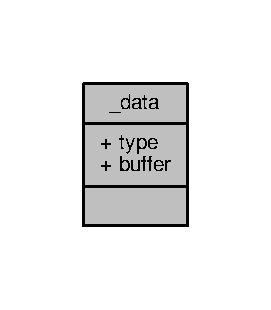
\includegraphics[width=130pt]{struct__data__coll__graph}
\end{center}
\end{figure}
\subsection*{Public Attributes}
\begin{DoxyCompactItemize}
\item 
int8\+\_\+t \hyperlink{struct__data_afa7c65aa86c5c877d1b23746b27f7ccd}{type}
\item 
char \hyperlink{struct__data_abcb37fabf89158d59a0469a376d2d5f8}{buffer} \mbox{[}\hyperlink{__data_8hpp_a6b20d41d6252e9871430c242cb1a56e7}{B\+U\+F\+F\+E\+R\+\_\+\+S\+I\+Z\+E}\mbox{]}
\end{DoxyCompactItemize}


\subsection{Member Data Documentation}
\hypertarget{struct__data_abcb37fabf89158d59a0469a376d2d5f8}{}\index{\+\_\+data@{\+\_\+data}!buffer@{buffer}}
\index{buffer@{buffer}!\+\_\+data@{\+\_\+data}}
\subsubsection[{buffer}]{\setlength{\rightskip}{0pt plus 5cm}char \+\_\+data\+::buffer\mbox{[}{\bf B\+U\+F\+F\+E\+R\+\_\+\+S\+I\+Z\+E}\mbox{]}}\label{struct__data_abcb37fabf89158d59a0469a376d2d5f8}
\hypertarget{struct__data_afa7c65aa86c5c877d1b23746b27f7ccd}{}\index{\+\_\+data@{\+\_\+data}!type@{type}}
\index{type@{type}!\+\_\+data@{\+\_\+data}}
\subsubsection[{type}]{\setlength{\rightskip}{0pt plus 5cm}int8\+\_\+t \+\_\+data\+::type}\label{struct__data_afa7c65aa86c5c877d1b23746b27f7ccd}


The documentation for this struct was generated from the following file\+:\begin{DoxyCompactItemize}
\item 
/home/clemente/projects/\+Troll-\/\+Killers/\hyperlink{__data_8hpp}{\+\_\+data.\+hpp}\end{DoxyCompactItemize}

\hypertarget{struct__msg}{}\section{\+\_\+msg Struct Reference}
\label{struct__msg}\index{\+\_\+msg@{\+\_\+msg}}


{\ttfamily \#include $<$Server.\+hpp$>$}



Collaboration diagram for \+\_\+msg\+:\nopagebreak
\begin{figure}[H]
\begin{center}
\leavevmode
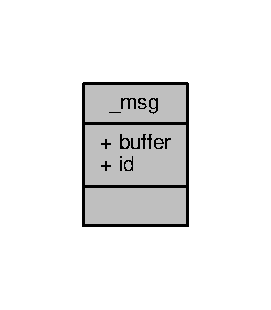
\includegraphics[width=130pt]{struct__msg__coll__graph}
\end{center}
\end{figure}
\subsection*{Public Attributes}
\begin{DoxyCompactItemize}
\item 
char \hyperlink{struct__msg_a470db8b42735763fc80e93590da2eaf4}{buffer} \mbox{[}\hyperlink{__data_8hpp_a6b20d41d6252e9871430c242cb1a56e7}{B\+U\+F\+F\+E\+R\+\_\+\+S\+I\+Z\+E}\mbox{]}
\item 
int \hyperlink{struct__msg_a5319cda008478b61e06ddf06c2cf166e}{id}
\end{DoxyCompactItemize}


\subsection{Member Data Documentation}
\hypertarget{struct__msg_a470db8b42735763fc80e93590da2eaf4}{}\index{\+\_\+msg@{\+\_\+msg}!buffer@{buffer}}
\index{buffer@{buffer}!\+\_\+msg@{\+\_\+msg}}
\subsubsection[{buffer}]{\setlength{\rightskip}{0pt plus 5cm}char \+\_\+msg\+::buffer\mbox{[}{\bf B\+U\+F\+F\+E\+R\+\_\+\+S\+I\+Z\+E}\mbox{]}}\label{struct__msg_a470db8b42735763fc80e93590da2eaf4}
\hypertarget{struct__msg_a5319cda008478b61e06ddf06c2cf166e}{}\index{\+\_\+msg@{\+\_\+msg}!id@{id}}
\index{id@{id}!\+\_\+msg@{\+\_\+msg}}
\subsubsection[{id}]{\setlength{\rightskip}{0pt plus 5cm}int \+\_\+msg\+::id}\label{struct__msg_a5319cda008478b61e06ddf06c2cf166e}


The documentation for this struct was generated from the following file\+:\begin{DoxyCompactItemize}
\item 
/home/clemente/projects/\+Troll-\/\+Killers/\hyperlink{_server_8hpp}{Server.\+hpp}\end{DoxyCompactItemize}

\hypertarget{struct__n_map}{}\section{\+\_\+n\+Map Struct Reference}
\label{struct__n_map}\index{\+\_\+n\+Map@{\+\_\+n\+Map}}


{\ttfamily \#include $<$Map.\+hpp$>$}



Collaboration diagram for \+\_\+n\+Map\+:\nopagebreak
\begin{figure}[H]
\begin{center}
\leavevmode
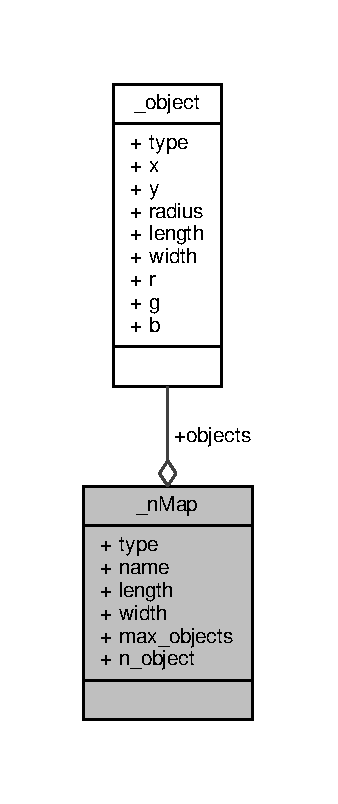
\includegraphics[width=162pt]{struct__n_map__coll__graph}
\end{center}
\end{figure}
\subsection*{Public Attributes}
\begin{DoxyCompactItemize}
\item 
int8\+\_\+t \hyperlink{struct__n_map_a79dda563cc2d4f715a9185f1a970150b}{type}
\item 
char \hyperlink{struct__n_map_a138f2aaca24cdaf5ec466c7889b21c15}{name} \mbox{[}50\mbox{]}
\item 
\hyperlink{struct__object}{\+\_\+object} $\ast$ \hyperlink{struct__n_map_ac3f3bf64347ac2accba1e388da7bfa07}{objects}
\item 
int16\+\_\+t \hyperlink{struct__n_map_a772868c89751c4a27a7eccf076df5fc6}{length}
\item 
int16\+\_\+t \hyperlink{struct__n_map_a4e83d0ff1af678de2d5b318e549d0ec5}{width}
\item 
int16\+\_\+t \hyperlink{struct__n_map_a4570178b4b02516d89d54fc7be2ccd4f}{max\+\_\+objects}
\item 
int16\+\_\+t \hyperlink{struct__n_map_ac41305de4abf61844a81b7a67992f2a8}{n\+\_\+object}
\end{DoxyCompactItemize}


\subsection{Member Data Documentation}
\hypertarget{struct__n_map_a772868c89751c4a27a7eccf076df5fc6}{}\index{\+\_\+n\+Map@{\+\_\+n\+Map}!length@{length}}
\index{length@{length}!\+\_\+n\+Map@{\+\_\+n\+Map}}
\subsubsection[{length}]{\setlength{\rightskip}{0pt plus 5cm}int16\+\_\+t \+\_\+n\+Map\+::length}\label{struct__n_map_a772868c89751c4a27a7eccf076df5fc6}
\hypertarget{struct__n_map_a4570178b4b02516d89d54fc7be2ccd4f}{}\index{\+\_\+n\+Map@{\+\_\+n\+Map}!max\+\_\+objects@{max\+\_\+objects}}
\index{max\+\_\+objects@{max\+\_\+objects}!\+\_\+n\+Map@{\+\_\+n\+Map}}
\subsubsection[{max\+\_\+objects}]{\setlength{\rightskip}{0pt plus 5cm}int16\+\_\+t \+\_\+n\+Map\+::max\+\_\+objects}\label{struct__n_map_a4570178b4b02516d89d54fc7be2ccd4f}
\hypertarget{struct__n_map_ac41305de4abf61844a81b7a67992f2a8}{}\index{\+\_\+n\+Map@{\+\_\+n\+Map}!n\+\_\+object@{n\+\_\+object}}
\index{n\+\_\+object@{n\+\_\+object}!\+\_\+n\+Map@{\+\_\+n\+Map}}
\subsubsection[{n\+\_\+object}]{\setlength{\rightskip}{0pt plus 5cm}int16\+\_\+t \+\_\+n\+Map\+::n\+\_\+object}\label{struct__n_map_ac41305de4abf61844a81b7a67992f2a8}
\hypertarget{struct__n_map_a138f2aaca24cdaf5ec466c7889b21c15}{}\index{\+\_\+n\+Map@{\+\_\+n\+Map}!name@{name}}
\index{name@{name}!\+\_\+n\+Map@{\+\_\+n\+Map}}
\subsubsection[{name}]{\setlength{\rightskip}{0pt plus 5cm}char \+\_\+n\+Map\+::name\mbox{[}50\mbox{]}}\label{struct__n_map_a138f2aaca24cdaf5ec466c7889b21c15}
\hypertarget{struct__n_map_ac3f3bf64347ac2accba1e388da7bfa07}{}\index{\+\_\+n\+Map@{\+\_\+n\+Map}!objects@{objects}}
\index{objects@{objects}!\+\_\+n\+Map@{\+\_\+n\+Map}}
\subsubsection[{objects}]{\setlength{\rightskip}{0pt plus 5cm}{\bf \+\_\+object}$\ast$ \+\_\+n\+Map\+::objects}\label{struct__n_map_ac3f3bf64347ac2accba1e388da7bfa07}
\hypertarget{struct__n_map_a79dda563cc2d4f715a9185f1a970150b}{}\index{\+\_\+n\+Map@{\+\_\+n\+Map}!type@{type}}
\index{type@{type}!\+\_\+n\+Map@{\+\_\+n\+Map}}
\subsubsection[{type}]{\setlength{\rightskip}{0pt plus 5cm}int8\+\_\+t \+\_\+n\+Map\+::type}\label{struct__n_map_a79dda563cc2d4f715a9185f1a970150b}
\hypertarget{struct__n_map_a4e83d0ff1af678de2d5b318e549d0ec5}{}\index{\+\_\+n\+Map@{\+\_\+n\+Map}!width@{width}}
\index{width@{width}!\+\_\+n\+Map@{\+\_\+n\+Map}}
\subsubsection[{width}]{\setlength{\rightskip}{0pt plus 5cm}int16\+\_\+t \+\_\+n\+Map\+::width}\label{struct__n_map_a4e83d0ff1af678de2d5b318e549d0ec5}


The documentation for this struct was generated from the following file\+:\begin{DoxyCompactItemize}
\item 
/home/clemente/projects/\+Troll-\/\+Killers/\hyperlink{_map_8hpp}{Map.\+hpp}\end{DoxyCompactItemize}

\hypertarget{struct__object}{}\section{\+\_\+object Struct Reference}
\label{struct__object}\index{\+\_\+object@{\+\_\+object}}


{\ttfamily \#include $<$\+\_\+object.\+hpp$>$}



Collaboration diagram for \+\_\+object\+:\nopagebreak
\begin{figure}[H]
\begin{center}
\leavevmode
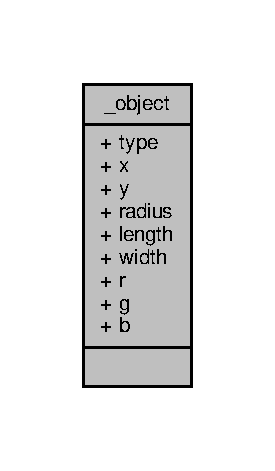
\includegraphics[width=132pt]{struct__object__coll__graph}
\end{center}
\end{figure}
\subsection*{Public Attributes}
\begin{DoxyCompactItemize}
\item 
int8\+\_\+t \hyperlink{struct__object_a4ffae0568ef6772f8ebefa0997f79243}{type}
\item 
int16\+\_\+t \hyperlink{struct__object_adb6e178c2aa0bc48f5db6d85106c1680}{x}
\item 
int16\+\_\+t \hyperlink{struct__object_a48f88904fef6cb2f4ea22029174d76bc}{y}
\item 
int16\+\_\+t \hyperlink{struct__object_a870a8b24b7b3dc9244f543f096e9dae6}{radius}
\item 
int16\+\_\+t \hyperlink{struct__object_a9d23dfa35b2571bf0b89d4ca75f5c155}{length}
\item 
int16\+\_\+t \hyperlink{struct__object_a7dff64a3cc71a49786c1052bb6c250ca}{width}
\item 
int16\+\_\+t \hyperlink{struct__object_af5318fcc501c7951e1bf261de6c29b3b}{r}
\item 
int16\+\_\+t \hyperlink{struct__object_a89ebce79c5f2acba52f871e6833977ff}{g}
\item 
int16\+\_\+t \hyperlink{struct__object_a104af22ae68294943efb54edb7a46b0e}{b}
\end{DoxyCompactItemize}


\subsection{Member Data Documentation}
\hypertarget{struct__object_a104af22ae68294943efb54edb7a46b0e}{}\index{\+\_\+object@{\+\_\+object}!b@{b}}
\index{b@{b}!\+\_\+object@{\+\_\+object}}
\subsubsection[{b}]{\setlength{\rightskip}{0pt plus 5cm}int16\+\_\+t \+\_\+object\+::b}\label{struct__object_a104af22ae68294943efb54edb7a46b0e}
\hypertarget{struct__object_a89ebce79c5f2acba52f871e6833977ff}{}\index{\+\_\+object@{\+\_\+object}!g@{g}}
\index{g@{g}!\+\_\+object@{\+\_\+object}}
\subsubsection[{g}]{\setlength{\rightskip}{0pt plus 5cm}int16\+\_\+t \+\_\+object\+::g}\label{struct__object_a89ebce79c5f2acba52f871e6833977ff}
\hypertarget{struct__object_a9d23dfa35b2571bf0b89d4ca75f5c155}{}\index{\+\_\+object@{\+\_\+object}!length@{length}}
\index{length@{length}!\+\_\+object@{\+\_\+object}}
\subsubsection[{length}]{\setlength{\rightskip}{0pt plus 5cm}int16\+\_\+t \+\_\+object\+::length}\label{struct__object_a9d23dfa35b2571bf0b89d4ca75f5c155}
\hypertarget{struct__object_af5318fcc501c7951e1bf261de6c29b3b}{}\index{\+\_\+object@{\+\_\+object}!r@{r}}
\index{r@{r}!\+\_\+object@{\+\_\+object}}
\subsubsection[{r}]{\setlength{\rightskip}{0pt plus 5cm}int16\+\_\+t \+\_\+object\+::r}\label{struct__object_af5318fcc501c7951e1bf261de6c29b3b}
\hypertarget{struct__object_a870a8b24b7b3dc9244f543f096e9dae6}{}\index{\+\_\+object@{\+\_\+object}!radius@{radius}}
\index{radius@{radius}!\+\_\+object@{\+\_\+object}}
\subsubsection[{radius}]{\setlength{\rightskip}{0pt plus 5cm}int16\+\_\+t \+\_\+object\+::radius}\label{struct__object_a870a8b24b7b3dc9244f543f096e9dae6}
\hypertarget{struct__object_a4ffae0568ef6772f8ebefa0997f79243}{}\index{\+\_\+object@{\+\_\+object}!type@{type}}
\index{type@{type}!\+\_\+object@{\+\_\+object}}
\subsubsection[{type}]{\setlength{\rightskip}{0pt plus 5cm}int8\+\_\+t \+\_\+object\+::type}\label{struct__object_a4ffae0568ef6772f8ebefa0997f79243}
\hypertarget{struct__object_a7dff64a3cc71a49786c1052bb6c250ca}{}\index{\+\_\+object@{\+\_\+object}!width@{width}}
\index{width@{width}!\+\_\+object@{\+\_\+object}}
\subsubsection[{width}]{\setlength{\rightskip}{0pt plus 5cm}int16\+\_\+t \+\_\+object\+::width}\label{struct__object_a7dff64a3cc71a49786c1052bb6c250ca}
\hypertarget{struct__object_adb6e178c2aa0bc48f5db6d85106c1680}{}\index{\+\_\+object@{\+\_\+object}!x@{x}}
\index{x@{x}!\+\_\+object@{\+\_\+object}}
\subsubsection[{x}]{\setlength{\rightskip}{0pt plus 5cm}int16\+\_\+t \+\_\+object\+::x}\label{struct__object_adb6e178c2aa0bc48f5db6d85106c1680}
\hypertarget{struct__object_a48f88904fef6cb2f4ea22029174d76bc}{}\index{\+\_\+object@{\+\_\+object}!y@{y}}
\index{y@{y}!\+\_\+object@{\+\_\+object}}
\subsubsection[{y}]{\setlength{\rightskip}{0pt plus 5cm}int16\+\_\+t \+\_\+object\+::y}\label{struct__object_a48f88904fef6cb2f4ea22029174d76bc}


The documentation for this struct was generated from the following file\+:\begin{DoxyCompactItemize}
\item 
/home/clemente/projects/\+Troll-\/\+Killers/\hyperlink{__object_8hpp}{\+\_\+object.\+hpp}\end{DoxyCompactItemize}

\hypertarget{class_c_character}{}\section{C\+Character Class Reference}
\label{class_c_character}\index{C\+Character@{C\+Character}}


{\ttfamily \#include $<$C\+Character.\+hpp$>$}



Inheritance diagram for C\+Character\+:\nopagebreak
\begin{figure}[H]
\begin{center}
\leavevmode
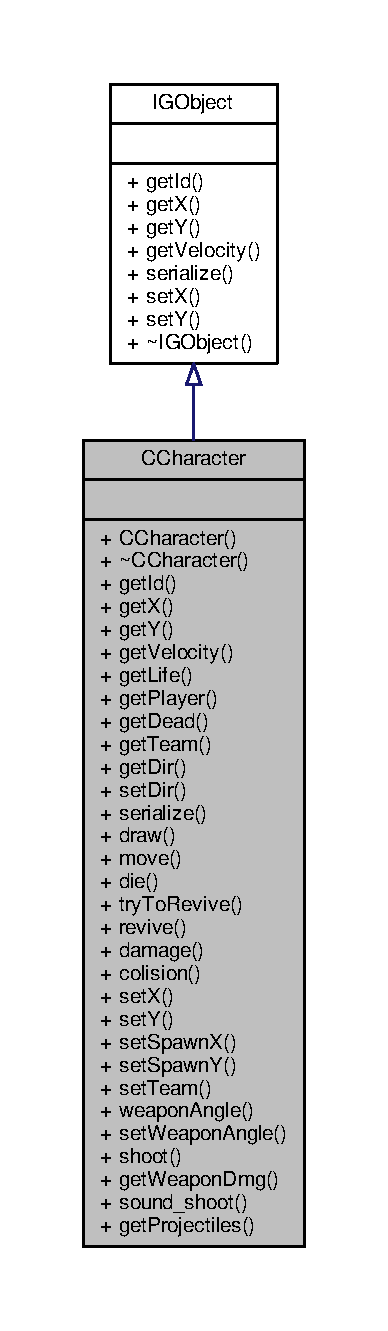
\includegraphics[height=550pt]{class_c_character__inherit__graph}
\end{center}
\end{figure}


Collaboration diagram for C\+Character\+:\nopagebreak
\begin{figure}[H]
\begin{center}
\leavevmode
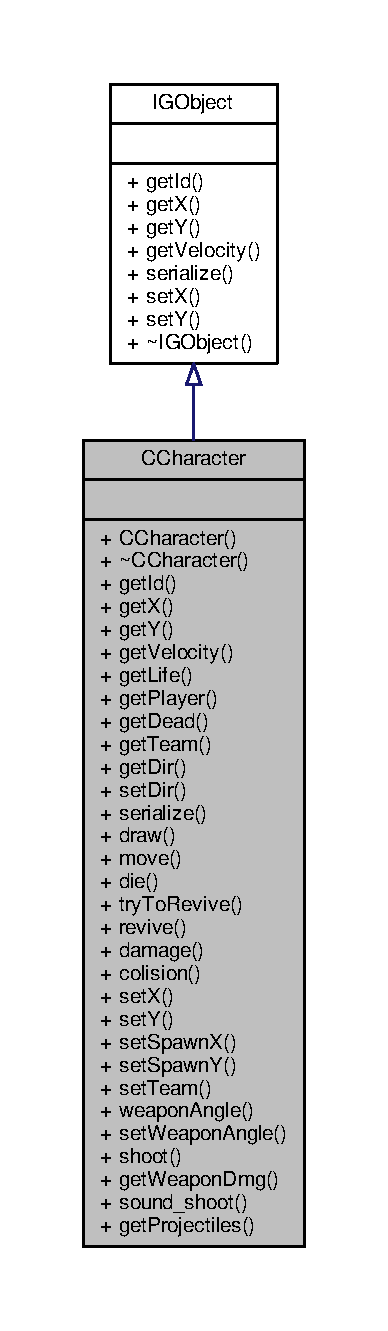
\includegraphics[height=550pt]{class_c_character__coll__graph}
\end{center}
\end{figure}
\subsection*{Public Member Functions}
\begin{DoxyCompactItemize}
\item 
\hyperlink{class_c_character_add20c9a63c5c11e8c0919e536d7636a2}{C\+Character} (\hyperlink{_enums_8hpp_ad9700e9db9d62004af4a04e4e13912c5}{Weapon} my\+Weapon)
\item 
\hyperlink{class_c_character_a8f8fb8991776a6b6a49c796e79968c91}{$\sim$\+C\+Character} ()
\item 
int16\+\_\+t \hyperlink{class_c_character_a317ea948f11c20c52b4eb915cbc6fd34}{get\+Id} ()
\item 
int16\+\_\+t \hyperlink{class_c_character_a27ef2164eae8c8858de7e22b8ae2b356}{get\+X} ()
\item 
int16\+\_\+t \hyperlink{class_c_character_a39af09fa51d180f49a58ffce78c9f25b}{get\+Y} ()
\item 
int16\+\_\+t \hyperlink{class_c_character_a7074f3d5a24d61766ce4d2fe354679ee}{get\+Velocity} ()
\item 
int \hyperlink{class_c_character_ae2e0ce8242ccb114248134e7d233fe80}{get\+Life} ()
\item 
\hyperlink{struct__object}{\+\_\+object} $\ast$ \hyperlink{class_c_character_af910f0944a8ba3afc92800fb696b7750}{get\+Player} ()
\item 
bool \hyperlink{class_c_character_aba453c8974f67b9a8621a63960263874}{get\+Dead} ()
\item 
\hyperlink{_enums_8hpp_a9c13bb5b1d69698f9b47900990eaa598}{Team} \hyperlink{class_c_character_a91ff320369ed4985b1c4b1762ce4fd9c}{get\+Team} ()
\item 
\hyperlink{_enums_8hpp_a224b9163917ac32fc95a60d8c1eec3aa}{Direction} \hyperlink{class_c_character_a367a85d8da544c05088712def127bf43}{get\+Dir} ()
\item 
void \hyperlink{class_c_character_a23914035239a49f1a2ce26248ce181f7}{set\+Dir} (\hyperlink{_enums_8hpp_a224b9163917ac32fc95a60d8c1eec3aa}{Direction} dir)
\item 
void \hyperlink{class_c_character_a2a9cb3e98cfe4c36ea292cdc38b999d8}{serialize} (char $\ast$buffer)
\item 
void \hyperlink{class_c_character_a80e38c97bd4d4fd9b7f017ec121f03a9}{draw} (int x, int y)
\item 
void \hyperlink{class_c_character_ad602f6042aeb6e500393bca375c4133b}{move} ()
\item 
void \hyperlink{class_c_character_adc71f8353440b2d5450938fa7c418aa7}{die} ()
\item 
bool \hyperlink{class_c_character_afe8285dd94fc52c099fb548840bc4e06}{try\+To\+Revive} ()
\item 
void \hyperlink{class_c_character_ad33d632d180cc5d487b0c39925caf278}{revive} (int16\+\_\+t x, int16\+\_\+t y)
\item 
void \hyperlink{class_c_character_a68c347ad267792fbed8ee9b1bae90967}{damage} (int dmg)
\item 
void \hyperlink{class_c_character_a84b44c9ef54291da3e28fb7f9dc05f20}{colision} (\hyperlink{struct__object}{\+\_\+object} $\ast$objects, int n)
\item 
void \hyperlink{class_c_character_a6d92d81e7bd039572e147ebe190fab6c}{set\+X} (int16\+\_\+t x)
\item 
void \hyperlink{class_c_character_a670de9c2ba79b716953a1dac2db9e4cf}{set\+Y} (int16\+\_\+t y)
\item 
void \hyperlink{class_c_character_abbabbe227437ea99b377e33c569da84c}{set\+Spawn\+X} (int16\+\_\+t x)
\item 
void \hyperlink{class_c_character_a0060a9e93f32488b4496545b9b3ef593}{set\+Spawn\+Y} (int16\+\_\+t y)
\item 
void \hyperlink{class_c_character_a4af37bf96b4950b67a538d1f5c1bc075}{set\+Team} (\hyperlink{_enums_8hpp_a9c13bb5b1d69698f9b47900990eaa598}{Team} team)
\item 
void \hyperlink{class_c_character_af64ec95c078f3e969cb6b961db81a488}{weapon\+Angle} (int map\+X, int map\+Y, int mouse\+X, int mouse\+Y)
\item 
void \hyperlink{class_c_character_a8aff509bd2bc8cb3eb7c3847533a3aed}{set\+Weapon\+Angle} (float angle)
\item 
void \hyperlink{class_c_character_a5fa507c6196ecc4132796dc250d7bb1d}{shoot} (A\+L\+L\+E\+G\+R\+O\+\_\+\+M\+O\+U\+S\+E\+\_\+\+S\+T\+A\+T\+E \&mouse\+State, \hyperlink{class_connection}{Connection} $\ast$conn)
\item 
int \hyperlink{class_c_character_ac7fd4192681975f1c1adf9933a7193b4}{get\+Weapon\+Dmg} ()
\item 
void \hyperlink{class_c_character_a98f733c8be0661e5e6b306d37a1dfeb5}{sound\+\_\+shoot} (int x, int y)
\item 
\hyperlink{class_projectile}{Projectile} $\ast$$\ast$ \hyperlink{class_c_character_a514a9a531863fe5ba308ec5805111e48}{get\+Projectiles} ()
\end{DoxyCompactItemize}


\subsection{Constructor \& Destructor Documentation}
\hypertarget{class_c_character_add20c9a63c5c11e8c0919e536d7636a2}{}\index{C\+Character@{C\+Character}!C\+Character@{C\+Character}}
\index{C\+Character@{C\+Character}!C\+Character@{C\+Character}}
\subsubsection[{C\+Character(\+Weapon my\+Weapon)}]{\setlength{\rightskip}{0pt plus 5cm}C\+Character\+::\+C\+Character (
\begin{DoxyParamCaption}
\item[{{\bf Weapon}}]{my\+Weapon}
\end{DoxyParamCaption}
)}\label{class_c_character_add20c9a63c5c11e8c0919e536d7636a2}


Here is the call graph for this function\+:\nopagebreak
\begin{figure}[H]
\begin{center}
\leavevmode
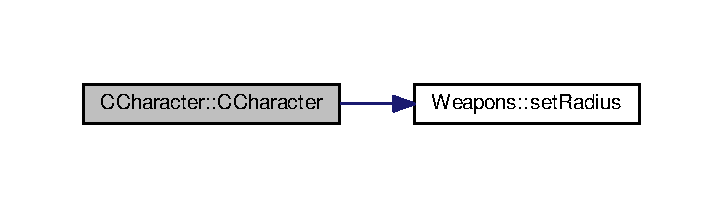
\includegraphics[width=347pt]{class_c_character_add20c9a63c5c11e8c0919e536d7636a2_cgraph}
\end{center}
\end{figure}


\hypertarget{class_c_character_a8f8fb8991776a6b6a49c796e79968c91}{}\index{C\+Character@{C\+Character}!````~C\+Character@{$\sim$\+C\+Character}}
\index{````~C\+Character@{$\sim$\+C\+Character}!C\+Character@{C\+Character}}
\subsubsection[{$\sim$\+C\+Character()}]{\setlength{\rightskip}{0pt plus 5cm}C\+Character\+::$\sim$\+C\+Character (
\begin{DoxyParamCaption}
{}
\end{DoxyParamCaption}
)}\label{class_c_character_a8f8fb8991776a6b6a49c796e79968c91}


\subsection{Member Function Documentation}
\hypertarget{class_c_character_a84b44c9ef54291da3e28fb7f9dc05f20}{}\index{C\+Character@{C\+Character}!colision@{colision}}
\index{colision@{colision}!C\+Character@{C\+Character}}
\subsubsection[{colision(\+\_\+object $\ast$objects, int n)}]{\setlength{\rightskip}{0pt plus 5cm}void C\+Character\+::colision (
\begin{DoxyParamCaption}
\item[{{\bf \+\_\+object} $\ast$}]{objects, }
\item[{int}]{n}
\end{DoxyParamCaption}
)}\label{class_c_character_a84b44c9ef54291da3e28fb7f9dc05f20}


Here is the call graph for this function\+:\nopagebreak
\begin{figure}[H]
\begin{center}
\leavevmode
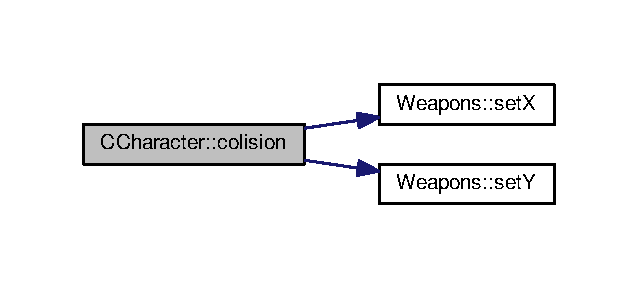
\includegraphics[width=306pt]{class_c_character_a84b44c9ef54291da3e28fb7f9dc05f20_cgraph}
\end{center}
\end{figure}




Here is the caller graph for this function\+:\nopagebreak
\begin{figure}[H]
\begin{center}
\leavevmode
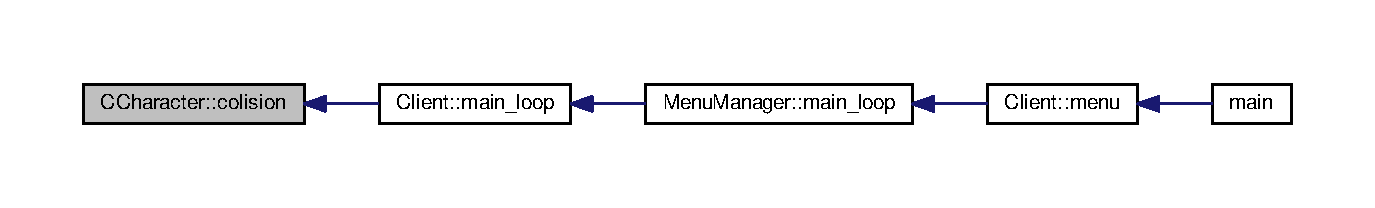
\includegraphics[width=350pt]{class_c_character_a84b44c9ef54291da3e28fb7f9dc05f20_icgraph}
\end{center}
\end{figure}


\hypertarget{class_c_character_a68c347ad267792fbed8ee9b1bae90967}{}\index{C\+Character@{C\+Character}!damage@{damage}}
\index{damage@{damage}!C\+Character@{C\+Character}}
\subsubsection[{damage(int dmg)}]{\setlength{\rightskip}{0pt plus 5cm}void C\+Character\+::damage (
\begin{DoxyParamCaption}
\item[{int}]{dmg}
\end{DoxyParamCaption}
)\hspace{0.3cm}{\ttfamily [inline]}}\label{class_c_character_a68c347ad267792fbed8ee9b1bae90967}


Here is the caller graph for this function\+:\nopagebreak
\begin{figure}[H]
\begin{center}
\leavevmode
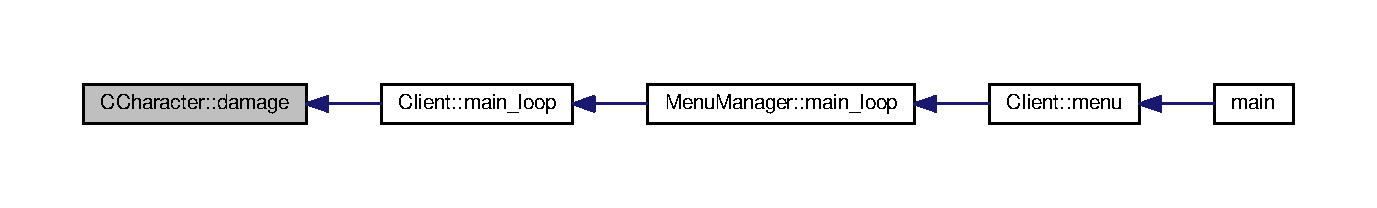
\includegraphics[width=350pt]{class_c_character_a68c347ad267792fbed8ee9b1bae90967_icgraph}
\end{center}
\end{figure}


\hypertarget{class_c_character_adc71f8353440b2d5450938fa7c418aa7}{}\index{C\+Character@{C\+Character}!die@{die}}
\index{die@{die}!C\+Character@{C\+Character}}
\subsubsection[{die()}]{\setlength{\rightskip}{0pt plus 5cm}void C\+Character\+::die (
\begin{DoxyParamCaption}
{}
\end{DoxyParamCaption}
)\hspace{0.3cm}{\ttfamily [inline]}}\label{class_c_character_adc71f8353440b2d5450938fa7c418aa7}


Here is the caller graph for this function\+:\nopagebreak
\begin{figure}[H]
\begin{center}
\leavevmode
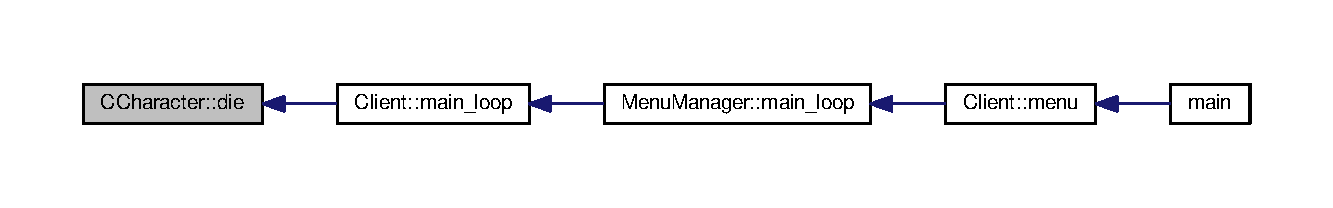
\includegraphics[width=350pt]{class_c_character_adc71f8353440b2d5450938fa7c418aa7_icgraph}
\end{center}
\end{figure}


\hypertarget{class_c_character_a80e38c97bd4d4fd9b7f017ec121f03a9}{}\index{C\+Character@{C\+Character}!draw@{draw}}
\index{draw@{draw}!C\+Character@{C\+Character}}
\subsubsection[{draw(int x, int y)}]{\setlength{\rightskip}{0pt plus 5cm}void C\+Character\+::draw (
\begin{DoxyParamCaption}
\item[{int}]{x, }
\item[{int}]{y}
\end{DoxyParamCaption}
)}\label{class_c_character_a80e38c97bd4d4fd9b7f017ec121f03a9}


Here is the call graph for this function\+:\nopagebreak
\begin{figure}[H]
\begin{center}
\leavevmode
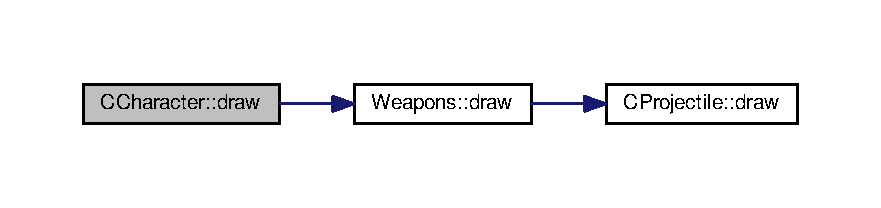
\includegraphics[width=350pt]{class_c_character_a80e38c97bd4d4fd9b7f017ec121f03a9_cgraph}
\end{center}
\end{figure}




Here is the caller graph for this function\+:\nopagebreak
\begin{figure}[H]
\begin{center}
\leavevmode
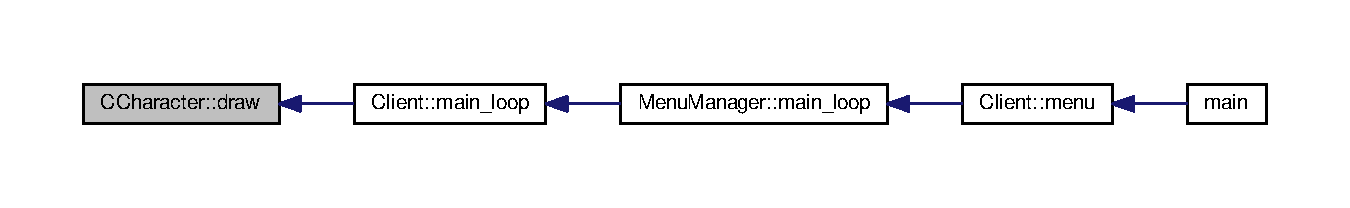
\includegraphics[width=350pt]{class_c_character_a80e38c97bd4d4fd9b7f017ec121f03a9_icgraph}
\end{center}
\end{figure}


\hypertarget{class_c_character_aba453c8974f67b9a8621a63960263874}{}\index{C\+Character@{C\+Character}!get\+Dead@{get\+Dead}}
\index{get\+Dead@{get\+Dead}!C\+Character@{C\+Character}}
\subsubsection[{get\+Dead()}]{\setlength{\rightskip}{0pt plus 5cm}bool C\+Character\+::get\+Dead (
\begin{DoxyParamCaption}
{}
\end{DoxyParamCaption}
)\hspace{0.3cm}{\ttfamily [inline]}}\label{class_c_character_aba453c8974f67b9a8621a63960263874}
\hypertarget{class_c_character_a367a85d8da544c05088712def127bf43}{}\index{C\+Character@{C\+Character}!get\+Dir@{get\+Dir}}
\index{get\+Dir@{get\+Dir}!C\+Character@{C\+Character}}
\subsubsection[{get\+Dir()}]{\setlength{\rightskip}{0pt plus 5cm}{\bf Direction} C\+Character\+::get\+Dir (
\begin{DoxyParamCaption}
{}
\end{DoxyParamCaption}
)\hspace{0.3cm}{\ttfamily [inline]}}\label{class_c_character_a367a85d8da544c05088712def127bf43}
\hypertarget{class_c_character_a317ea948f11c20c52b4eb915cbc6fd34}{}\index{C\+Character@{C\+Character}!get\+Id@{get\+Id}}
\index{get\+Id@{get\+Id}!C\+Character@{C\+Character}}
\subsubsection[{get\+Id()}]{\setlength{\rightskip}{0pt plus 5cm}int16\+\_\+t C\+Character\+::get\+Id (
\begin{DoxyParamCaption}
{}
\end{DoxyParamCaption}
)\hspace{0.3cm}{\ttfamily [inline]}, {\ttfamily [virtual]}}\label{class_c_character_a317ea948f11c20c52b4eb915cbc6fd34}


Implements \hyperlink{class_i_g_object_a40fdbe0db5e995e22996567d77bf45c6}{I\+G\+Object}.

\hypertarget{class_c_character_ae2e0ce8242ccb114248134e7d233fe80}{}\index{C\+Character@{C\+Character}!get\+Life@{get\+Life}}
\index{get\+Life@{get\+Life}!C\+Character@{C\+Character}}
\subsubsection[{get\+Life()}]{\setlength{\rightskip}{0pt plus 5cm}int C\+Character\+::get\+Life (
\begin{DoxyParamCaption}
{}
\end{DoxyParamCaption}
)\hspace{0.3cm}{\ttfamily [inline]}}\label{class_c_character_ae2e0ce8242ccb114248134e7d233fe80}
\hypertarget{class_c_character_af910f0944a8ba3afc92800fb696b7750}{}\index{C\+Character@{C\+Character}!get\+Player@{get\+Player}}
\index{get\+Player@{get\+Player}!C\+Character@{C\+Character}}
\subsubsection[{get\+Player()}]{\setlength{\rightskip}{0pt plus 5cm}{\bf \+\_\+object}$\ast$ C\+Character\+::get\+Player (
\begin{DoxyParamCaption}
{}
\end{DoxyParamCaption}
)\hspace{0.3cm}{\ttfamily [inline]}}\label{class_c_character_af910f0944a8ba3afc92800fb696b7750}


Here is the caller graph for this function\+:\nopagebreak
\begin{figure}[H]
\begin{center}
\leavevmode
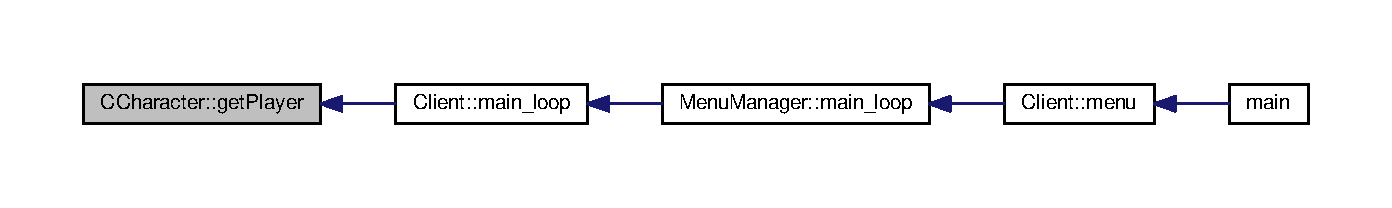
\includegraphics[width=350pt]{class_c_character_af910f0944a8ba3afc92800fb696b7750_icgraph}
\end{center}
\end{figure}


\hypertarget{class_c_character_a514a9a531863fe5ba308ec5805111e48}{}\index{C\+Character@{C\+Character}!get\+Projectiles@{get\+Projectiles}}
\index{get\+Projectiles@{get\+Projectiles}!C\+Character@{C\+Character}}
\subsubsection[{get\+Projectiles()}]{\setlength{\rightskip}{0pt plus 5cm}{\bf Projectile}$\ast$$\ast$ C\+Character\+::get\+Projectiles (
\begin{DoxyParamCaption}
{}
\end{DoxyParamCaption}
)\hspace{0.3cm}{\ttfamily [inline]}}\label{class_c_character_a514a9a531863fe5ba308ec5805111e48}


Here is the call graph for this function\+:\nopagebreak
\begin{figure}[H]
\begin{center}
\leavevmode
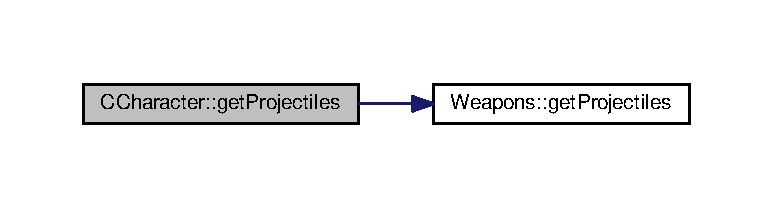
\includegraphics[width=350pt]{class_c_character_a514a9a531863fe5ba308ec5805111e48_cgraph}
\end{center}
\end{figure}




Here is the caller graph for this function\+:\nopagebreak
\begin{figure}[H]
\begin{center}
\leavevmode
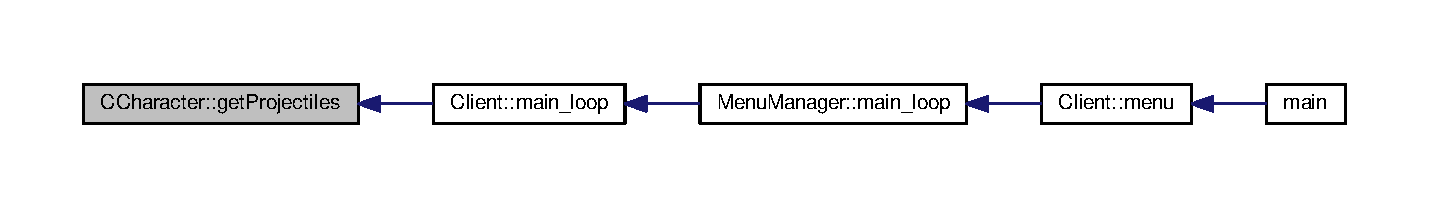
\includegraphics[width=350pt]{class_c_character_a514a9a531863fe5ba308ec5805111e48_icgraph}
\end{center}
\end{figure}


\hypertarget{class_c_character_a91ff320369ed4985b1c4b1762ce4fd9c}{}\index{C\+Character@{C\+Character}!get\+Team@{get\+Team}}
\index{get\+Team@{get\+Team}!C\+Character@{C\+Character}}
\subsubsection[{get\+Team()}]{\setlength{\rightskip}{0pt plus 5cm}{\bf Team} C\+Character\+::get\+Team (
\begin{DoxyParamCaption}
{}
\end{DoxyParamCaption}
)\hspace{0.3cm}{\ttfamily [inline]}}\label{class_c_character_a91ff320369ed4985b1c4b1762ce4fd9c}
\hypertarget{class_c_character_a7074f3d5a24d61766ce4d2fe354679ee}{}\index{C\+Character@{C\+Character}!get\+Velocity@{get\+Velocity}}
\index{get\+Velocity@{get\+Velocity}!C\+Character@{C\+Character}}
\subsubsection[{get\+Velocity()}]{\setlength{\rightskip}{0pt plus 5cm}int16\+\_\+t C\+Character\+::get\+Velocity (
\begin{DoxyParamCaption}
{}
\end{DoxyParamCaption}
)\hspace{0.3cm}{\ttfamily [inline]}, {\ttfamily [virtual]}}\label{class_c_character_a7074f3d5a24d61766ce4d2fe354679ee}


Implements \hyperlink{class_i_g_object_afc8764ec832e6a60c58dace401d65b32}{I\+G\+Object}.

\hypertarget{class_c_character_ac7fd4192681975f1c1adf9933a7193b4}{}\index{C\+Character@{C\+Character}!get\+Weapon\+Dmg@{get\+Weapon\+Dmg}}
\index{get\+Weapon\+Dmg@{get\+Weapon\+Dmg}!C\+Character@{C\+Character}}
\subsubsection[{get\+Weapon\+Dmg()}]{\setlength{\rightskip}{0pt plus 5cm}int C\+Character\+::get\+Weapon\+Dmg (
\begin{DoxyParamCaption}
{}
\end{DoxyParamCaption}
)\hspace{0.3cm}{\ttfamily [inline]}}\label{class_c_character_ac7fd4192681975f1c1adf9933a7193b4}


Here is the call graph for this function\+:\nopagebreak
\begin{figure}[H]
\begin{center}
\leavevmode
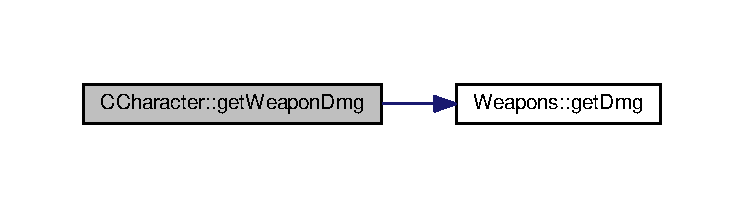
\includegraphics[width=350pt]{class_c_character_ac7fd4192681975f1c1adf9933a7193b4_cgraph}
\end{center}
\end{figure}




Here is the caller graph for this function\+:\nopagebreak
\begin{figure}[H]
\begin{center}
\leavevmode
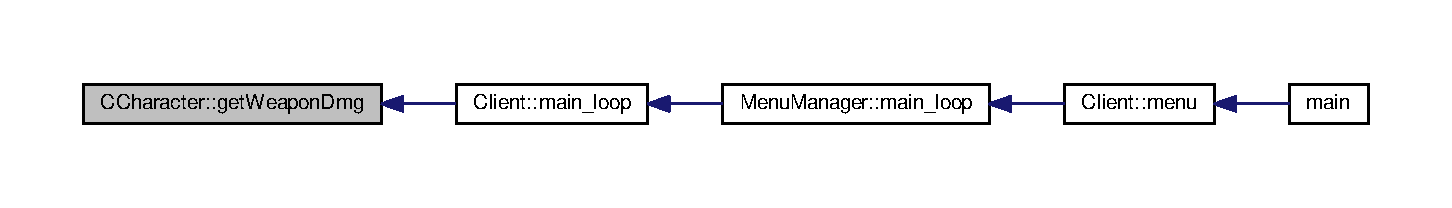
\includegraphics[width=350pt]{class_c_character_ac7fd4192681975f1c1adf9933a7193b4_icgraph}
\end{center}
\end{figure}


\hypertarget{class_c_character_a27ef2164eae8c8858de7e22b8ae2b356}{}\index{C\+Character@{C\+Character}!get\+X@{get\+X}}
\index{get\+X@{get\+X}!C\+Character@{C\+Character}}
\subsubsection[{get\+X()}]{\setlength{\rightskip}{0pt plus 5cm}int16\+\_\+t C\+Character\+::get\+X (
\begin{DoxyParamCaption}
{}
\end{DoxyParamCaption}
)\hspace{0.3cm}{\ttfamily [inline]}, {\ttfamily [virtual]}}\label{class_c_character_a27ef2164eae8c8858de7e22b8ae2b356}


Implements \hyperlink{class_i_g_object_aa6ae1f7bd99277a3558a8e90d833fa7a}{I\+G\+Object}.



Here is the caller graph for this function\+:\nopagebreak
\begin{figure}[H]
\begin{center}
\leavevmode
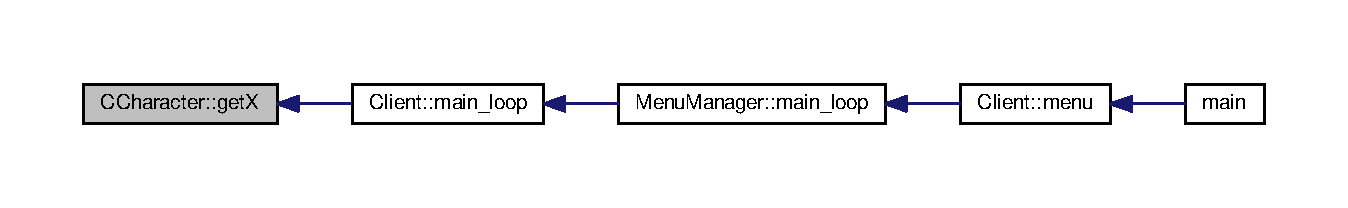
\includegraphics[width=350pt]{class_c_character_a27ef2164eae8c8858de7e22b8ae2b356_icgraph}
\end{center}
\end{figure}


\hypertarget{class_c_character_a39af09fa51d180f49a58ffce78c9f25b}{}\index{C\+Character@{C\+Character}!get\+Y@{get\+Y}}
\index{get\+Y@{get\+Y}!C\+Character@{C\+Character}}
\subsubsection[{get\+Y()}]{\setlength{\rightskip}{0pt plus 5cm}int16\+\_\+t C\+Character\+::get\+Y (
\begin{DoxyParamCaption}
{}
\end{DoxyParamCaption}
)\hspace{0.3cm}{\ttfamily [inline]}, {\ttfamily [virtual]}}\label{class_c_character_a39af09fa51d180f49a58ffce78c9f25b}


Implements \hyperlink{class_i_g_object_a3491bdb3a6b6ba8d66e07443a5b5951d}{I\+G\+Object}.



Here is the caller graph for this function\+:\nopagebreak
\begin{figure}[H]
\begin{center}
\leavevmode
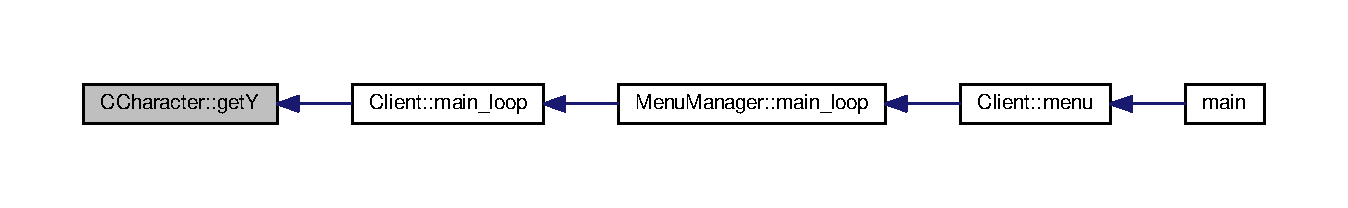
\includegraphics[width=350pt]{class_c_character_a39af09fa51d180f49a58ffce78c9f25b_icgraph}
\end{center}
\end{figure}


\hypertarget{class_c_character_ad602f6042aeb6e500393bca375c4133b}{}\index{C\+Character@{C\+Character}!move@{move}}
\index{move@{move}!C\+Character@{C\+Character}}
\subsubsection[{move()}]{\setlength{\rightskip}{0pt plus 5cm}void C\+Character\+::move (
\begin{DoxyParamCaption}
{}
\end{DoxyParamCaption}
)}\label{class_c_character_ad602f6042aeb6e500393bca375c4133b}


Here is the call graph for this function\+:\nopagebreak
\begin{figure}[H]
\begin{center}
\leavevmode
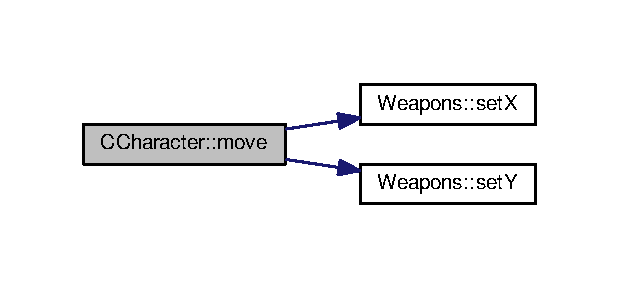
\includegraphics[width=297pt]{class_c_character_ad602f6042aeb6e500393bca375c4133b_cgraph}
\end{center}
\end{figure}




Here is the caller graph for this function\+:\nopagebreak
\begin{figure}[H]
\begin{center}
\leavevmode
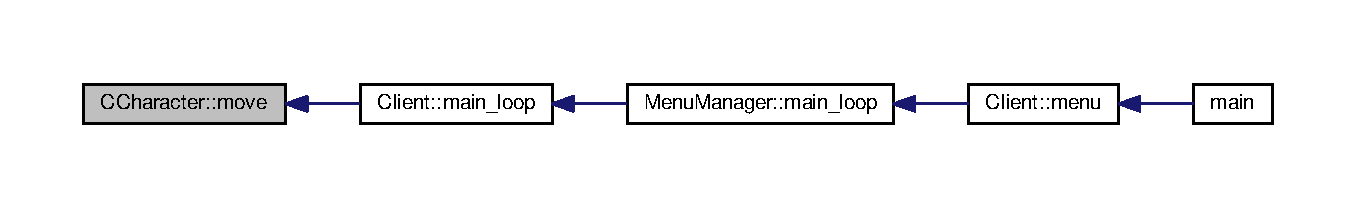
\includegraphics[width=350pt]{class_c_character_ad602f6042aeb6e500393bca375c4133b_icgraph}
\end{center}
\end{figure}


\hypertarget{class_c_character_ad33d632d180cc5d487b0c39925caf278}{}\index{C\+Character@{C\+Character}!revive@{revive}}
\index{revive@{revive}!C\+Character@{C\+Character}}
\subsubsection[{revive(int16\+\_\+t x, int16\+\_\+t y)}]{\setlength{\rightskip}{0pt plus 5cm}void C\+Character\+::revive (
\begin{DoxyParamCaption}
\item[{int16\+\_\+t}]{x, }
\item[{int16\+\_\+t}]{y}
\end{DoxyParamCaption}
)}\label{class_c_character_ad33d632d180cc5d487b0c39925caf278}


Here is the call graph for this function\+:\nopagebreak
\begin{figure}[H]
\begin{center}
\leavevmode
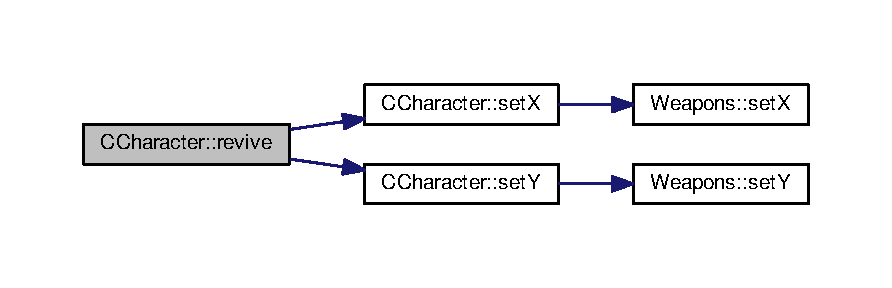
\includegraphics[width=350pt]{class_c_character_ad33d632d180cc5d487b0c39925caf278_cgraph}
\end{center}
\end{figure}




Here is the caller graph for this function\+:\nopagebreak
\begin{figure}[H]
\begin{center}
\leavevmode
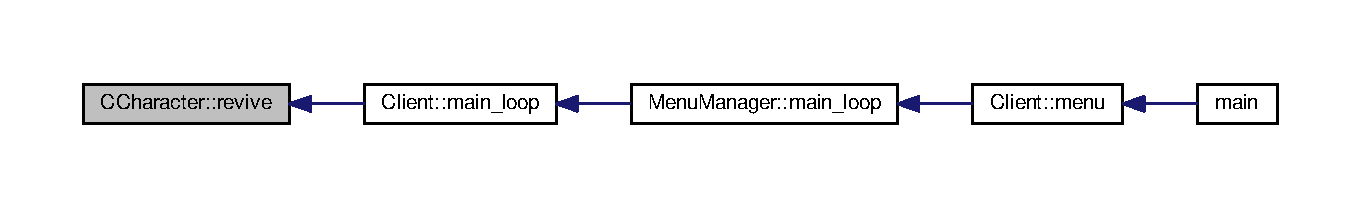
\includegraphics[width=350pt]{class_c_character_ad33d632d180cc5d487b0c39925caf278_icgraph}
\end{center}
\end{figure}


\hypertarget{class_c_character_a2a9cb3e98cfe4c36ea292cdc38b999d8}{}\index{C\+Character@{C\+Character}!serialize@{serialize}}
\index{serialize@{serialize}!C\+Character@{C\+Character}}
\subsubsection[{serialize(char $\ast$buffer)}]{\setlength{\rightskip}{0pt plus 5cm}void C\+Character\+::serialize (
\begin{DoxyParamCaption}
\item[{char $\ast$}]{buffer}
\end{DoxyParamCaption}
)\hspace{0.3cm}{\ttfamily [virtual]}}\label{class_c_character_a2a9cb3e98cfe4c36ea292cdc38b999d8}


Implements \hyperlink{class_i_g_object_a6e2dd93acb47fc77668e2571bff3481e}{I\+G\+Object}.



Here is the call graph for this function\+:\nopagebreak
\begin{figure}[H]
\begin{center}
\leavevmode
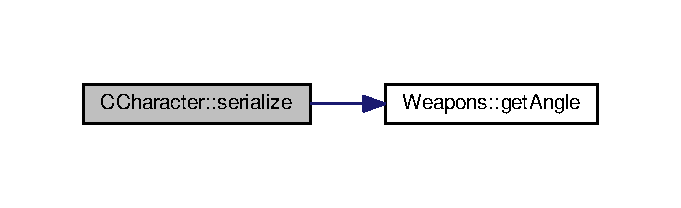
\includegraphics[width=327pt]{class_c_character_a2a9cb3e98cfe4c36ea292cdc38b999d8_cgraph}
\end{center}
\end{figure}




Here is the caller graph for this function\+:\nopagebreak
\begin{figure}[H]
\begin{center}
\leavevmode
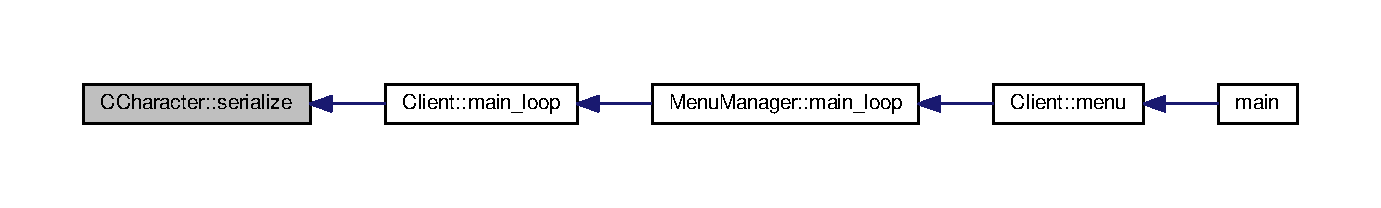
\includegraphics[width=350pt]{class_c_character_a2a9cb3e98cfe4c36ea292cdc38b999d8_icgraph}
\end{center}
\end{figure}


\hypertarget{class_c_character_a23914035239a49f1a2ce26248ce181f7}{}\index{C\+Character@{C\+Character}!set\+Dir@{set\+Dir}}
\index{set\+Dir@{set\+Dir}!C\+Character@{C\+Character}}
\subsubsection[{set\+Dir(\+Direction dir)}]{\setlength{\rightskip}{0pt plus 5cm}void C\+Character\+::set\+Dir (
\begin{DoxyParamCaption}
\item[{{\bf Direction}}]{dir}
\end{DoxyParamCaption}
)\hspace{0.3cm}{\ttfamily [inline]}}\label{class_c_character_a23914035239a49f1a2ce26248ce181f7}


Here is the caller graph for this function\+:\nopagebreak
\begin{figure}[H]
\begin{center}
\leavevmode
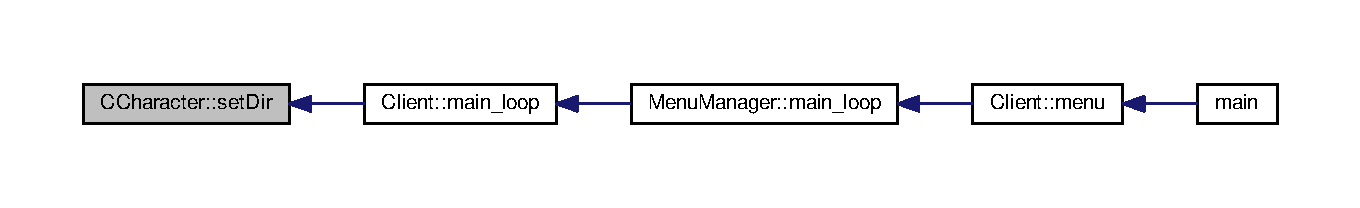
\includegraphics[width=350pt]{class_c_character_a23914035239a49f1a2ce26248ce181f7_icgraph}
\end{center}
\end{figure}


\hypertarget{class_c_character_abbabbe227437ea99b377e33c569da84c}{}\index{C\+Character@{C\+Character}!set\+Spawn\+X@{set\+Spawn\+X}}
\index{set\+Spawn\+X@{set\+Spawn\+X}!C\+Character@{C\+Character}}
\subsubsection[{set\+Spawn\+X(int16\+\_\+t x)}]{\setlength{\rightskip}{0pt plus 5cm}void C\+Character\+::set\+Spawn\+X (
\begin{DoxyParamCaption}
\item[{int16\+\_\+t}]{x}
\end{DoxyParamCaption}
)\hspace{0.3cm}{\ttfamily [inline]}}\label{class_c_character_abbabbe227437ea99b377e33c569da84c}


Here is the caller graph for this function\+:\nopagebreak
\begin{figure}[H]
\begin{center}
\leavevmode
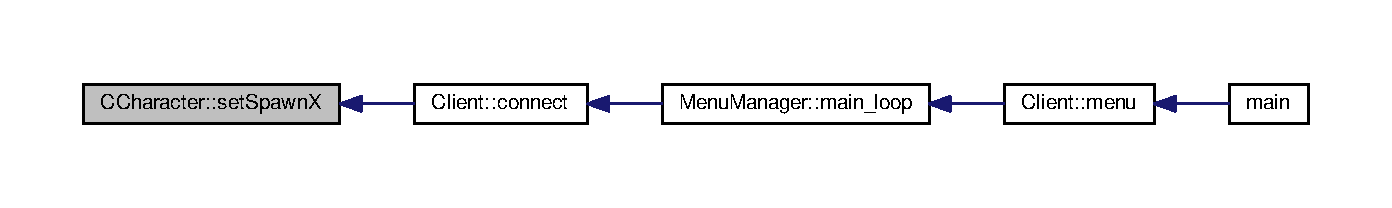
\includegraphics[width=350pt]{class_c_character_abbabbe227437ea99b377e33c569da84c_icgraph}
\end{center}
\end{figure}


\hypertarget{class_c_character_a0060a9e93f32488b4496545b9b3ef593}{}\index{C\+Character@{C\+Character}!set\+Spawn\+Y@{set\+Spawn\+Y}}
\index{set\+Spawn\+Y@{set\+Spawn\+Y}!C\+Character@{C\+Character}}
\subsubsection[{set\+Spawn\+Y(int16\+\_\+t y)}]{\setlength{\rightskip}{0pt plus 5cm}void C\+Character\+::set\+Spawn\+Y (
\begin{DoxyParamCaption}
\item[{int16\+\_\+t}]{y}
\end{DoxyParamCaption}
)\hspace{0.3cm}{\ttfamily [inline]}}\label{class_c_character_a0060a9e93f32488b4496545b9b3ef593}


Here is the caller graph for this function\+:\nopagebreak
\begin{figure}[H]
\begin{center}
\leavevmode
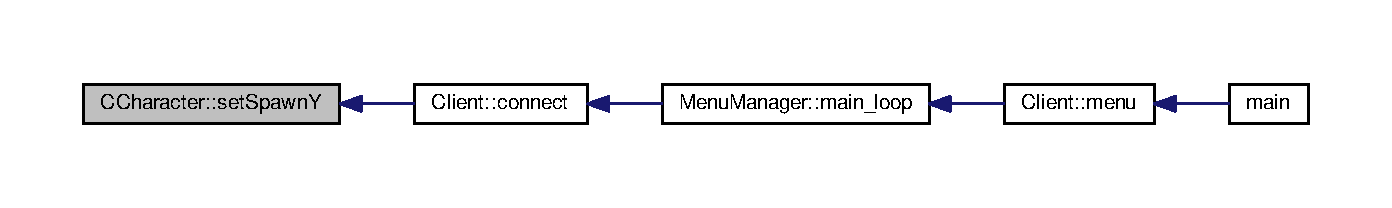
\includegraphics[width=350pt]{class_c_character_a0060a9e93f32488b4496545b9b3ef593_icgraph}
\end{center}
\end{figure}


\hypertarget{class_c_character_a4af37bf96b4950b67a538d1f5c1bc075}{}\index{C\+Character@{C\+Character}!set\+Team@{set\+Team}}
\index{set\+Team@{set\+Team}!C\+Character@{C\+Character}}
\subsubsection[{set\+Team(\+Team team)}]{\setlength{\rightskip}{0pt plus 5cm}void C\+Character\+::set\+Team (
\begin{DoxyParamCaption}
\item[{{\bf Team}}]{team}
\end{DoxyParamCaption}
)}\label{class_c_character_a4af37bf96b4950b67a538d1f5c1bc075}


Here is the caller graph for this function\+:\nopagebreak
\begin{figure}[H]
\begin{center}
\leavevmode
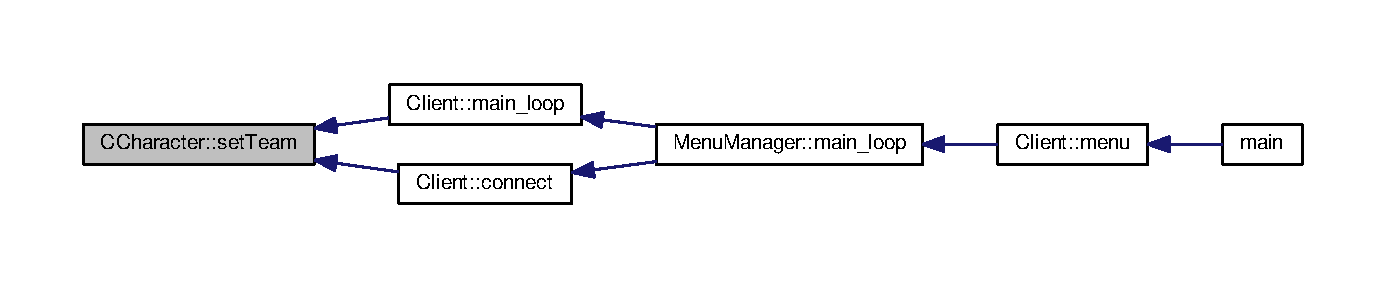
\includegraphics[width=350pt]{class_c_character_a4af37bf96b4950b67a538d1f5c1bc075_icgraph}
\end{center}
\end{figure}


\hypertarget{class_c_character_a8aff509bd2bc8cb3eb7c3847533a3aed}{}\index{C\+Character@{C\+Character}!set\+Weapon\+Angle@{set\+Weapon\+Angle}}
\index{set\+Weapon\+Angle@{set\+Weapon\+Angle}!C\+Character@{C\+Character}}
\subsubsection[{set\+Weapon\+Angle(float angle)}]{\setlength{\rightskip}{0pt plus 5cm}void C\+Character\+::set\+Weapon\+Angle (
\begin{DoxyParamCaption}
\item[{float}]{angle}
\end{DoxyParamCaption}
)\hspace{0.3cm}{\ttfamily [inline]}}\label{class_c_character_a8aff509bd2bc8cb3eb7c3847533a3aed}


Here is the call graph for this function\+:\nopagebreak
\begin{figure}[H]
\begin{center}
\leavevmode
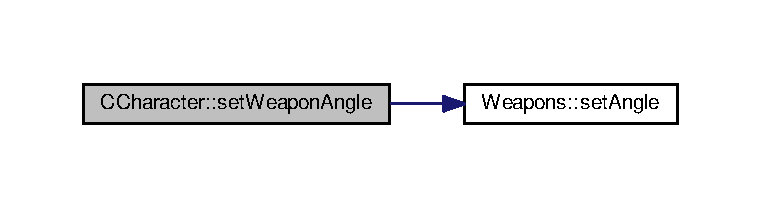
\includegraphics[width=350pt]{class_c_character_a8aff509bd2bc8cb3eb7c3847533a3aed_cgraph}
\end{center}
\end{figure}




Here is the caller graph for this function\+:\nopagebreak
\begin{figure}[H]
\begin{center}
\leavevmode
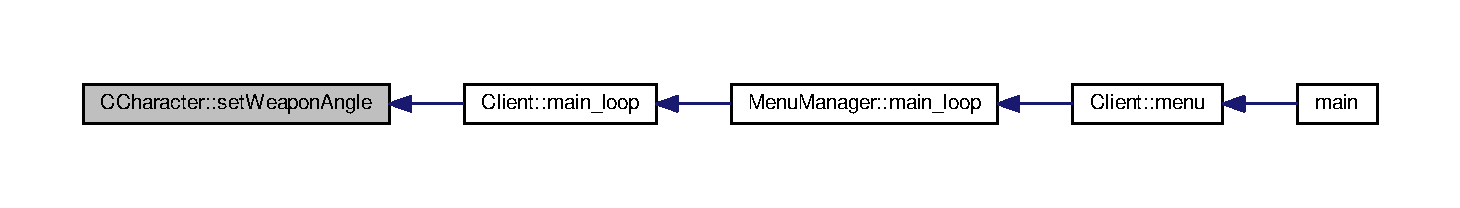
\includegraphics[width=350pt]{class_c_character_a8aff509bd2bc8cb3eb7c3847533a3aed_icgraph}
\end{center}
\end{figure}


\hypertarget{class_c_character_a6d92d81e7bd039572e147ebe190fab6c}{}\index{C\+Character@{C\+Character}!set\+X@{set\+X}}
\index{set\+X@{set\+X}!C\+Character@{C\+Character}}
\subsubsection[{set\+X(int16\+\_\+t x)}]{\setlength{\rightskip}{0pt plus 5cm}void C\+Character\+::set\+X (
\begin{DoxyParamCaption}
\item[{int16\+\_\+t}]{x}
\end{DoxyParamCaption}
)\hspace{0.3cm}{\ttfamily [inline]}, {\ttfamily [virtual]}}\label{class_c_character_a6d92d81e7bd039572e147ebe190fab6c}


Implements \hyperlink{class_i_g_object_a4b810d1b4a785d7532104113ef5cf0ba}{I\+G\+Object}.



Here is the call graph for this function\+:\nopagebreak
\begin{figure}[H]
\begin{center}
\leavevmode
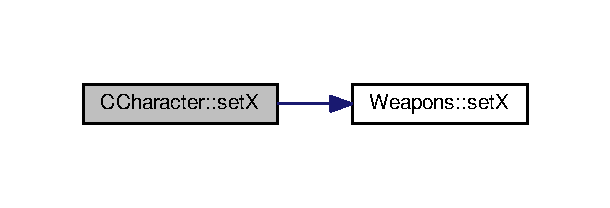
\includegraphics[width=293pt]{class_c_character_a6d92d81e7bd039572e147ebe190fab6c_cgraph}
\end{center}
\end{figure}




Here is the caller graph for this function\+:\nopagebreak
\begin{figure}[H]
\begin{center}
\leavevmode
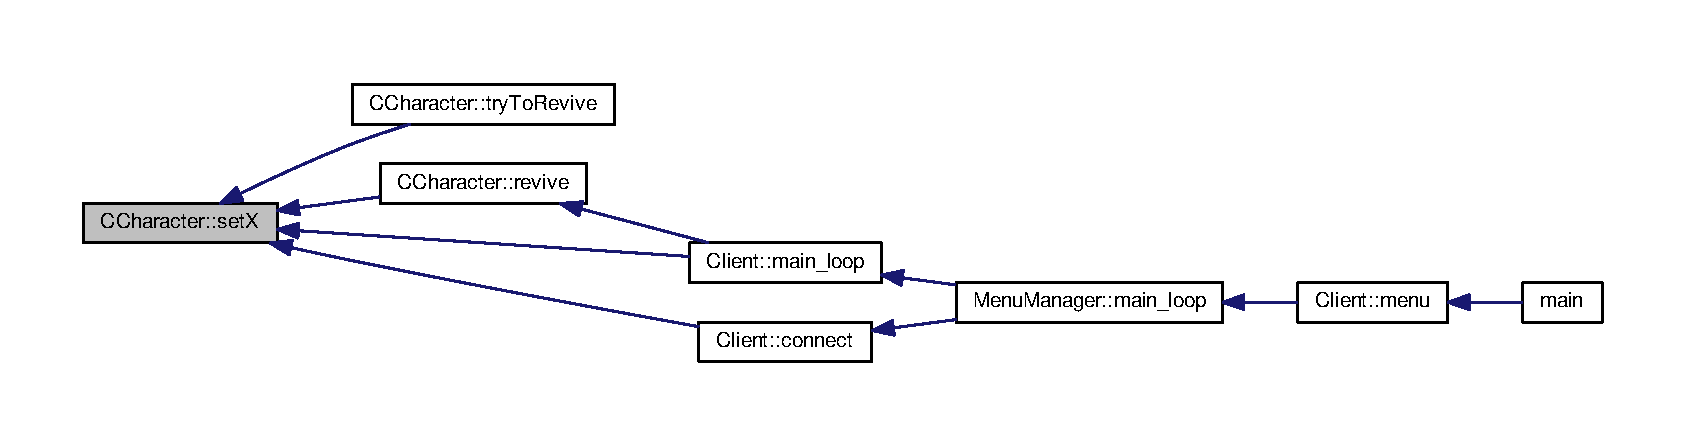
\includegraphics[width=350pt]{class_c_character_a6d92d81e7bd039572e147ebe190fab6c_icgraph}
\end{center}
\end{figure}


\hypertarget{class_c_character_a670de9c2ba79b716953a1dac2db9e4cf}{}\index{C\+Character@{C\+Character}!set\+Y@{set\+Y}}
\index{set\+Y@{set\+Y}!C\+Character@{C\+Character}}
\subsubsection[{set\+Y(int16\+\_\+t y)}]{\setlength{\rightskip}{0pt plus 5cm}void C\+Character\+::set\+Y (
\begin{DoxyParamCaption}
\item[{int16\+\_\+t}]{y}
\end{DoxyParamCaption}
)\hspace{0.3cm}{\ttfamily [inline]}, {\ttfamily [virtual]}}\label{class_c_character_a670de9c2ba79b716953a1dac2db9e4cf}


Implements \hyperlink{class_i_g_object_a5092ff8b79a61c3856510adb0543f229}{I\+G\+Object}.



Here is the call graph for this function\+:\nopagebreak
\begin{figure}[H]
\begin{center}
\leavevmode
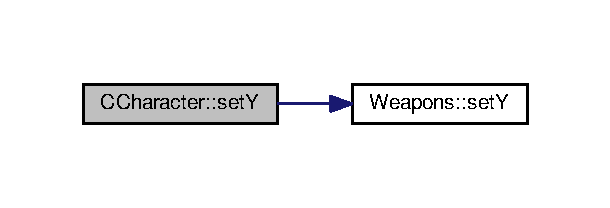
\includegraphics[width=293pt]{class_c_character_a670de9c2ba79b716953a1dac2db9e4cf_cgraph}
\end{center}
\end{figure}




Here is the caller graph for this function\+:\nopagebreak
\begin{figure}[H]
\begin{center}
\leavevmode
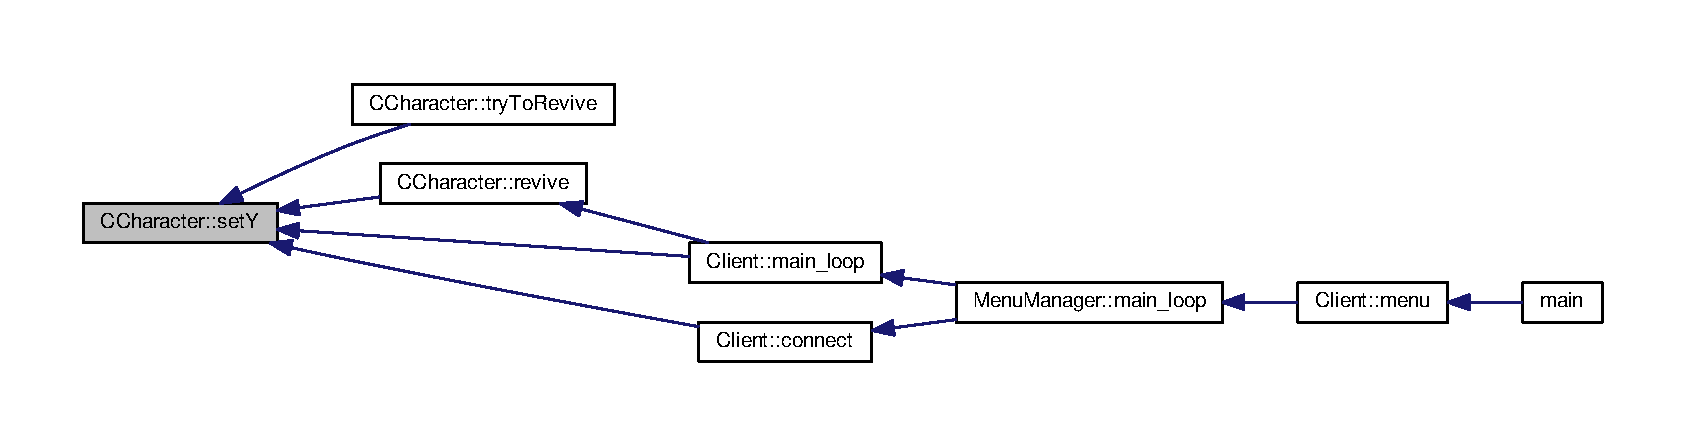
\includegraphics[width=350pt]{class_c_character_a670de9c2ba79b716953a1dac2db9e4cf_icgraph}
\end{center}
\end{figure}


\hypertarget{class_c_character_a5fa507c6196ecc4132796dc250d7bb1d}{}\index{C\+Character@{C\+Character}!shoot@{shoot}}
\index{shoot@{shoot}!C\+Character@{C\+Character}}
\subsubsection[{shoot(\+A\+L\+L\+E\+G\+R\+O\+\_\+\+M\+O\+U\+S\+E\+\_\+\+S\+T\+A\+T\+E \&mouse\+State, Connection $\ast$conn)}]{\setlength{\rightskip}{0pt plus 5cm}void C\+Character\+::shoot (
\begin{DoxyParamCaption}
\item[{A\+L\+L\+E\+G\+R\+O\+\_\+\+M\+O\+U\+S\+E\+\_\+\+S\+T\+A\+T\+E \&}]{mouse\+State, }
\item[{{\bf Connection} $\ast$}]{conn}
\end{DoxyParamCaption}
)\hspace{0.3cm}{\ttfamily [inline]}}\label{class_c_character_a5fa507c6196ecc4132796dc250d7bb1d}


Here is the call graph for this function\+:\nopagebreak
\begin{figure}[H]
\begin{center}
\leavevmode
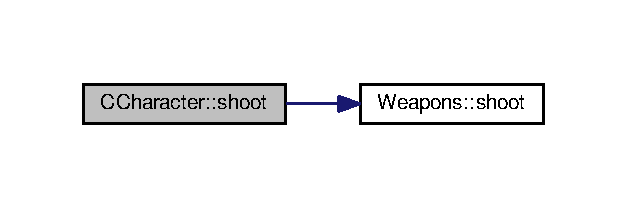
\includegraphics[width=301pt]{class_c_character_a5fa507c6196ecc4132796dc250d7bb1d_cgraph}
\end{center}
\end{figure}




Here is the caller graph for this function\+:\nopagebreak
\begin{figure}[H]
\begin{center}
\leavevmode
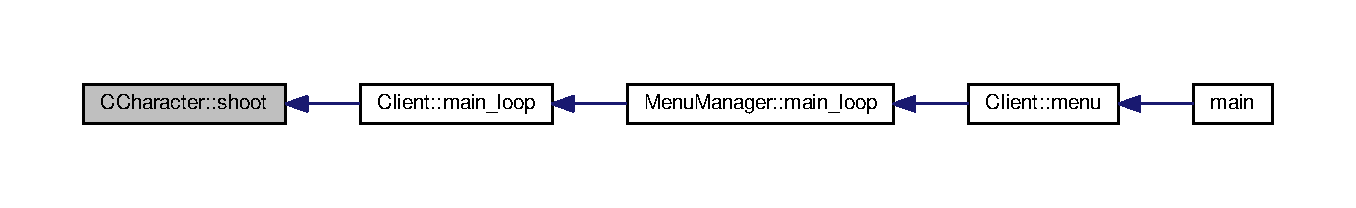
\includegraphics[width=350pt]{class_c_character_a5fa507c6196ecc4132796dc250d7bb1d_icgraph}
\end{center}
\end{figure}


\hypertarget{class_c_character_a98f733c8be0661e5e6b306d37a1dfeb5}{}\index{C\+Character@{C\+Character}!sound\+\_\+shoot@{sound\+\_\+shoot}}
\index{sound\+\_\+shoot@{sound\+\_\+shoot}!C\+Character@{C\+Character}}
\subsubsection[{sound\+\_\+shoot(int x, int y)}]{\setlength{\rightskip}{0pt plus 5cm}void C\+Character\+::sound\+\_\+shoot (
\begin{DoxyParamCaption}
\item[{int}]{x, }
\item[{int}]{y}
\end{DoxyParamCaption}
)}\label{class_c_character_a98f733c8be0661e5e6b306d37a1dfeb5}


Here is the call graph for this function\+:\nopagebreak
\begin{figure}[H]
\begin{center}
\leavevmode
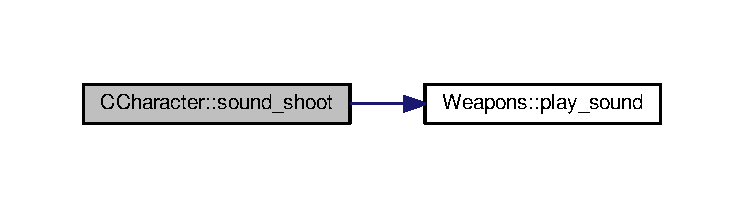
\includegraphics[width=350pt]{class_c_character_a98f733c8be0661e5e6b306d37a1dfeb5_cgraph}
\end{center}
\end{figure}




Here is the caller graph for this function\+:\nopagebreak
\begin{figure}[H]
\begin{center}
\leavevmode
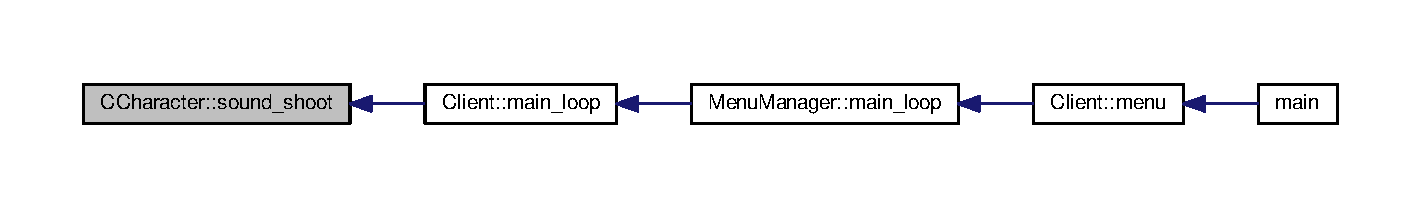
\includegraphics[width=350pt]{class_c_character_a98f733c8be0661e5e6b306d37a1dfeb5_icgraph}
\end{center}
\end{figure}


\hypertarget{class_c_character_afe8285dd94fc52c099fb548840bc4e06}{}\index{C\+Character@{C\+Character}!try\+To\+Revive@{try\+To\+Revive}}
\index{try\+To\+Revive@{try\+To\+Revive}!C\+Character@{C\+Character}}
\subsubsection[{try\+To\+Revive()}]{\setlength{\rightskip}{0pt plus 5cm}bool C\+Character\+::try\+To\+Revive (
\begin{DoxyParamCaption}
{}
\end{DoxyParamCaption}
)}\label{class_c_character_afe8285dd94fc52c099fb548840bc4e06}


Here is the call graph for this function\+:\nopagebreak
\begin{figure}[H]
\begin{center}
\leavevmode
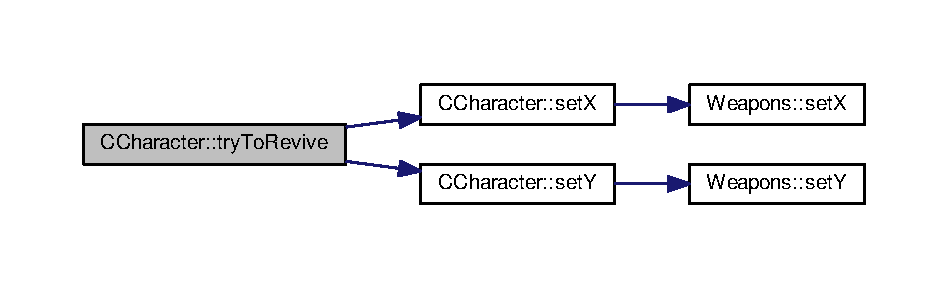
\includegraphics[width=350pt]{class_c_character_afe8285dd94fc52c099fb548840bc4e06_cgraph}
\end{center}
\end{figure}


\hypertarget{class_c_character_af64ec95c078f3e969cb6b961db81a488}{}\index{C\+Character@{C\+Character}!weapon\+Angle@{weapon\+Angle}}
\index{weapon\+Angle@{weapon\+Angle}!C\+Character@{C\+Character}}
\subsubsection[{weapon\+Angle(int map\+X, int map\+Y, int mouse\+X, int mouse\+Y)}]{\setlength{\rightskip}{0pt plus 5cm}void C\+Character\+::weapon\+Angle (
\begin{DoxyParamCaption}
\item[{int}]{map\+X, }
\item[{int}]{map\+Y, }
\item[{int}]{mouse\+X, }
\item[{int}]{mouse\+Y}
\end{DoxyParamCaption}
)}\label{class_c_character_af64ec95c078f3e969cb6b961db81a488}


Here is the call graph for this function\+:\nopagebreak
\begin{figure}[H]
\begin{center}
\leavevmode
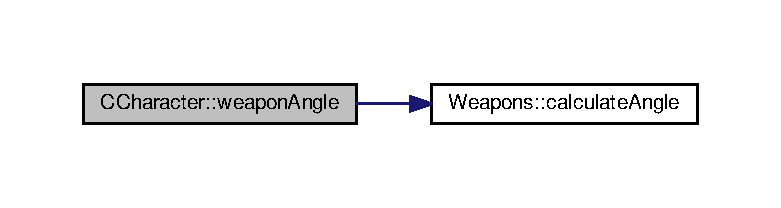
\includegraphics[width=350pt]{class_c_character_af64ec95c078f3e969cb6b961db81a488_cgraph}
\end{center}
\end{figure}




Here is the caller graph for this function\+:\nopagebreak
\begin{figure}[H]
\begin{center}
\leavevmode
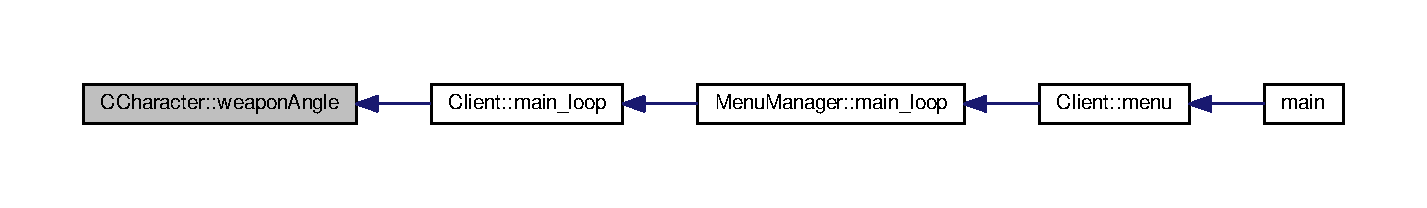
\includegraphics[width=350pt]{class_c_character_af64ec95c078f3e969cb6b961db81a488_icgraph}
\end{center}
\end{figure}




The documentation for this class was generated from the following files\+:\begin{DoxyCompactItemize}
\item 
/home/clemente/projects/\+Troll-\/\+Killers/\hyperlink{_c_character_8hpp}{C\+Character.\+hpp}\item 
/home/clemente/projects/\+Troll-\/\+Killers/\hyperlink{_c_character_8cpp}{C\+Character.\+cpp}\end{DoxyCompactItemize}

\hypertarget{class_client}{}\section{Client Class Reference}
\label{class_client}\index{Client@{Client}}


{\ttfamily \#include $<$Client.\+hpp$>$}



Collaboration diagram for Client\+:\nopagebreak
\begin{figure}[H]
\begin{center}
\leavevmode
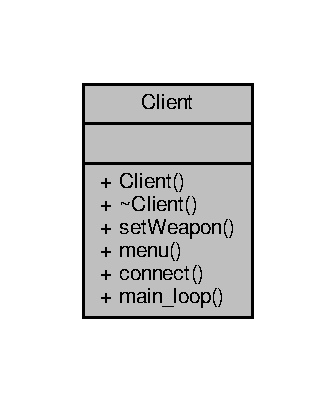
\includegraphics[width=161pt]{class_client__coll__graph}
\end{center}
\end{figure}
\subsection*{Public Member Functions}
\begin{DoxyCompactItemize}
\item 
\hyperlink{class_client_ae51af7aa6b8f591496a8f6a4a87a14bf}{Client} ()
\item 
\hyperlink{class_client_a840e519ca781888cbd54181572ebe3a7}{$\sim$\+Client} ()
\item 
void \hyperlink{class_client_ab8104db60235ae805fb77a8cb161c4b8}{set\+Weapon} (\hyperlink{_enums_8hpp_ad9700e9db9d62004af4a04e4e13912c5}{Weapon} my\+Weapon)
\item 
void \hyperlink{class_client_a8a2de145bff51cff643e5a8d773d35fe}{menu} ()
\item 
bool \hyperlink{class_client_abccb976632db0b3b5df925875b80b2e7}{connect} ()
\item 
void \hyperlink{class_client_a9fbb2f61b005ee6ab3f73b9f449d95eb}{main\+\_\+loop} ()
\end{DoxyCompactItemize}


\subsection{Constructor \& Destructor Documentation}
\hypertarget{class_client_ae51af7aa6b8f591496a8f6a4a87a14bf}{}\index{Client@{Client}!Client@{Client}}
\index{Client@{Client}!Client@{Client}}
\subsubsection[{Client()}]{\setlength{\rightskip}{0pt plus 5cm}Client\+::\+Client (
\begin{DoxyParamCaption}
{}
\end{DoxyParamCaption}
)}\label{class_client_ae51af7aa6b8f591496a8f6a4a87a14bf}


Here is the call graph for this function\+:\nopagebreak
\begin{figure}[H]
\begin{center}
\leavevmode
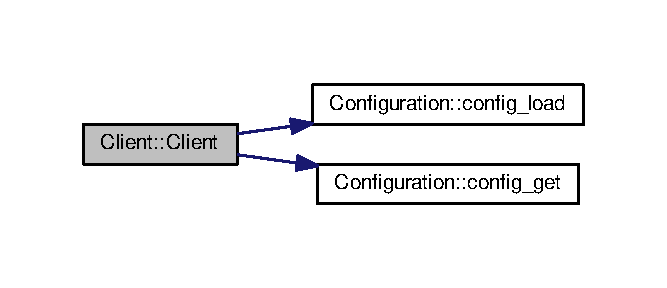
\includegraphics[width=320pt]{class_client_ae51af7aa6b8f591496a8f6a4a87a14bf_cgraph}
\end{center}
\end{figure}


\hypertarget{class_client_a840e519ca781888cbd54181572ebe3a7}{}\index{Client@{Client}!````~Client@{$\sim$\+Client}}
\index{````~Client@{$\sim$\+Client}!Client@{Client}}
\subsubsection[{$\sim$\+Client()}]{\setlength{\rightskip}{0pt plus 5cm}Client\+::$\sim$\+Client (
\begin{DoxyParamCaption}
{}
\end{DoxyParamCaption}
)}\label{class_client_a840e519ca781888cbd54181572ebe3a7}


\subsection{Member Function Documentation}
\hypertarget{class_client_abccb976632db0b3b5df925875b80b2e7}{}\index{Client@{Client}!connect@{connect}}
\index{connect@{connect}!Client@{Client}}
\subsubsection[{connect()}]{\setlength{\rightskip}{0pt plus 5cm}bool Client\+::connect (
\begin{DoxyParamCaption}
{}
\end{DoxyParamCaption}
)}\label{class_client_abccb976632db0b3b5df925875b80b2e7}


Here is the call graph for this function\+:\nopagebreak
\begin{figure}[H]
\begin{center}
\leavevmode
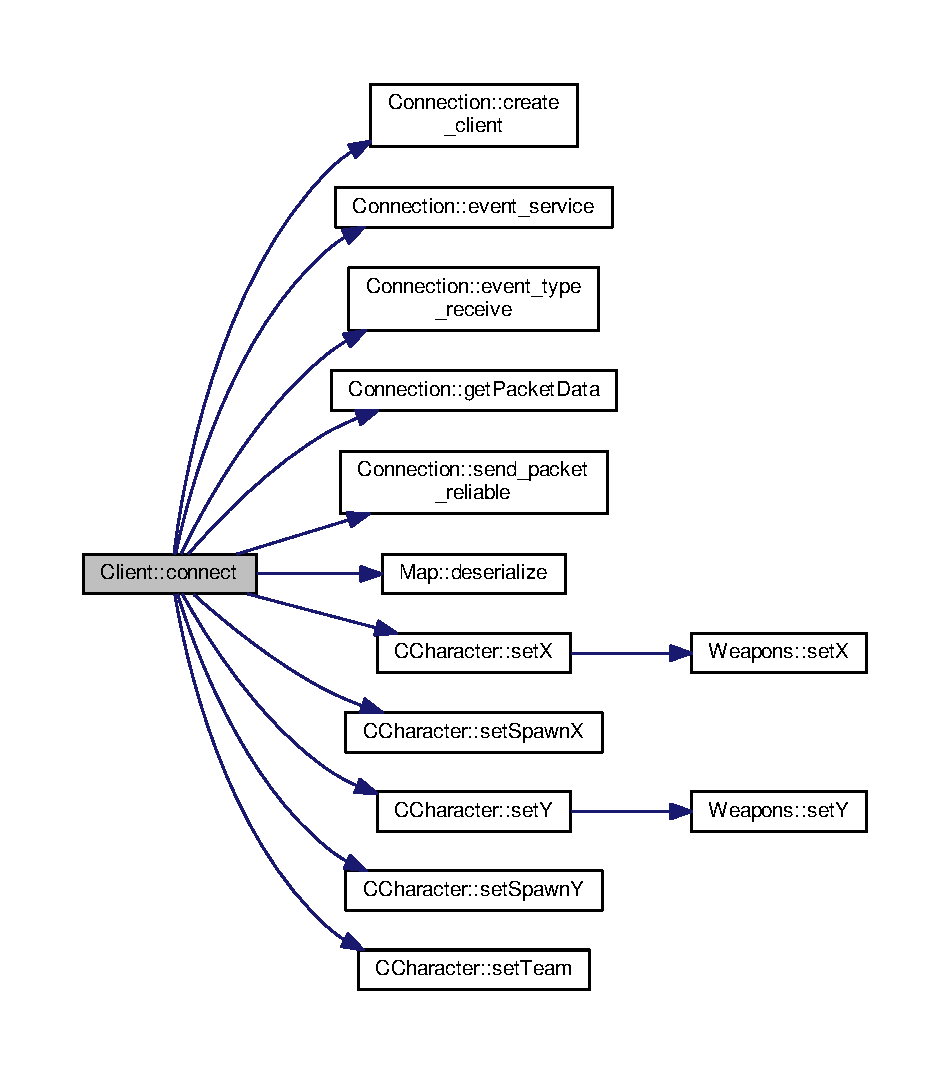
\includegraphics[width=350pt]{class_client_abccb976632db0b3b5df925875b80b2e7_cgraph}
\end{center}
\end{figure}




Here is the caller graph for this function\+:\nopagebreak
\begin{figure}[H]
\begin{center}
\leavevmode
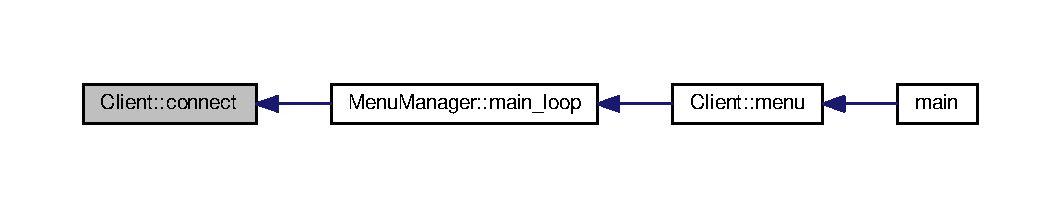
\includegraphics[width=350pt]{class_client_abccb976632db0b3b5df925875b80b2e7_icgraph}
\end{center}
\end{figure}


\hypertarget{class_client_a9fbb2f61b005ee6ab3f73b9f449d95eb}{}\index{Client@{Client}!main\+\_\+loop@{main\+\_\+loop}}
\index{main\+\_\+loop@{main\+\_\+loop}!Client@{Client}}
\subsubsection[{main\+\_\+loop()}]{\setlength{\rightskip}{0pt plus 5cm}void Client\+::main\+\_\+loop (
\begin{DoxyParamCaption}
{}
\end{DoxyParamCaption}
)}\label{class_client_a9fbb2f61b005ee6ab3f73b9f449d95eb}


Here is the call graph for this function\+:\nopagebreak
\begin{figure}[H]
\begin{center}
\leavevmode
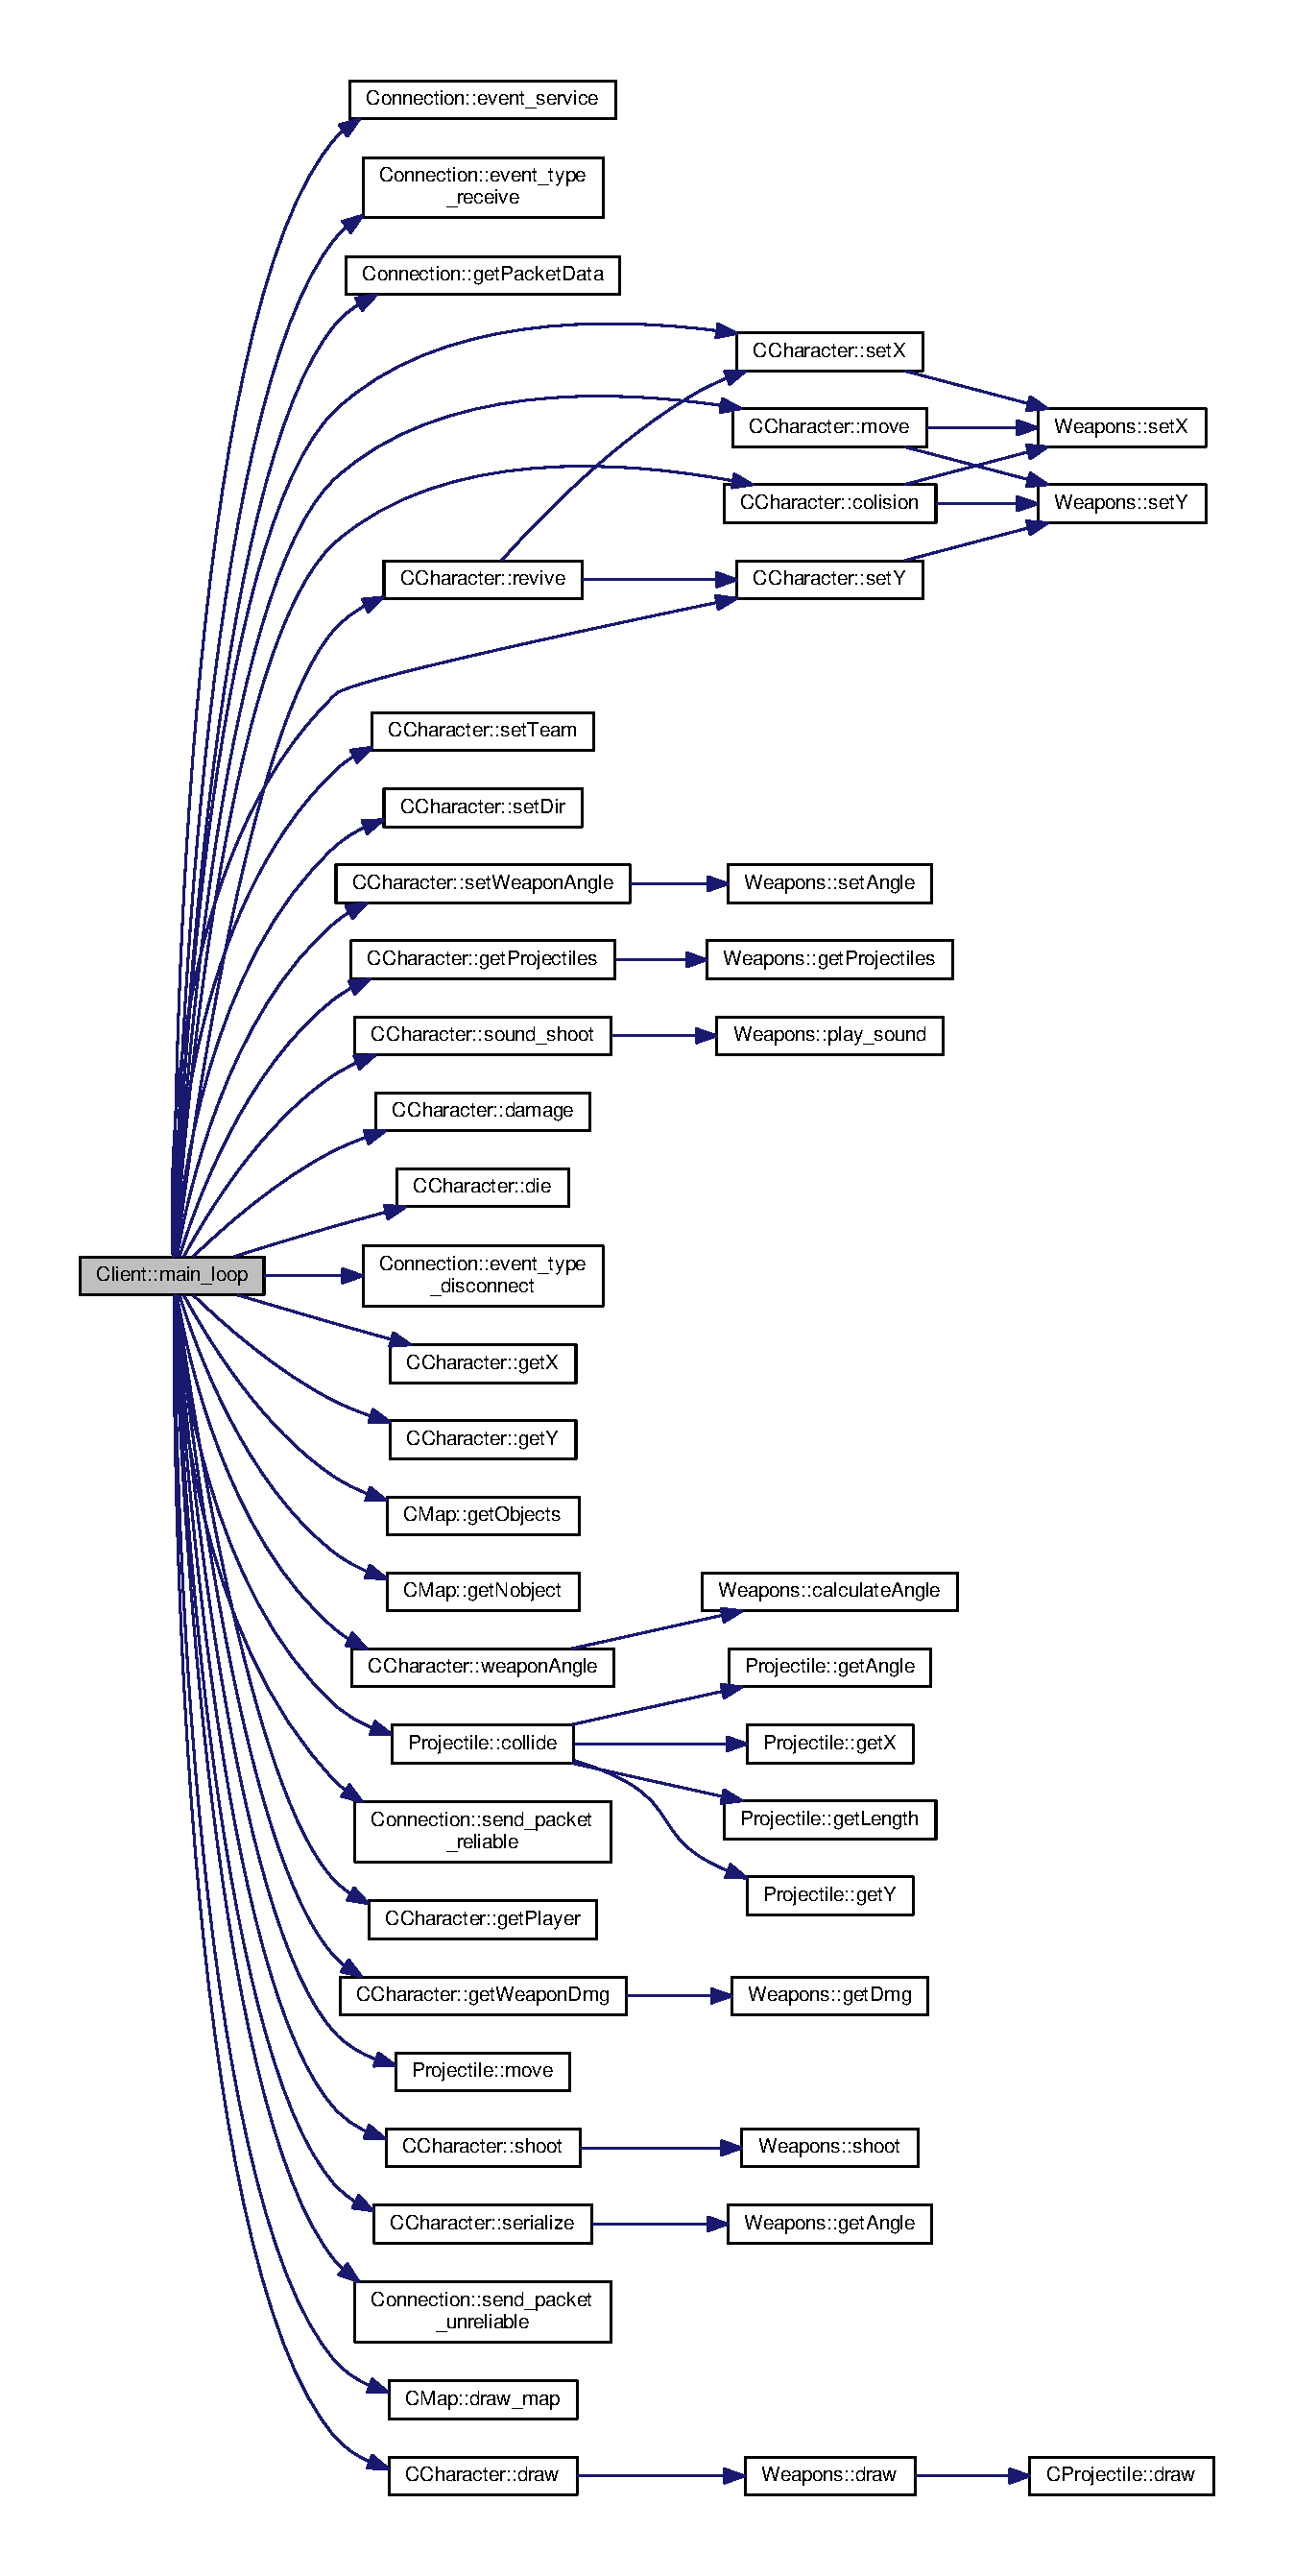
\includegraphics[height=550pt]{class_client_a9fbb2f61b005ee6ab3f73b9f449d95eb_cgraph}
\end{center}
\end{figure}




Here is the caller graph for this function\+:\nopagebreak
\begin{figure}[H]
\begin{center}
\leavevmode
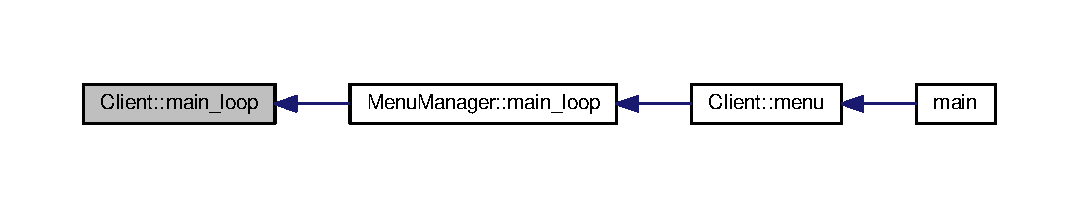
\includegraphics[width=350pt]{class_client_a9fbb2f61b005ee6ab3f73b9f449d95eb_icgraph}
\end{center}
\end{figure}


\hypertarget{class_client_a8a2de145bff51cff643e5a8d773d35fe}{}\index{Client@{Client}!menu@{menu}}
\index{menu@{menu}!Client@{Client}}
\subsubsection[{menu()}]{\setlength{\rightskip}{0pt plus 5cm}void Client\+::menu (
\begin{DoxyParamCaption}
{}
\end{DoxyParamCaption}
)\hspace{0.3cm}{\ttfamily [inline]}}\label{class_client_a8a2de145bff51cff643e5a8d773d35fe}


Here is the call graph for this function\+:\nopagebreak
\begin{figure}[H]
\begin{center}
\leavevmode
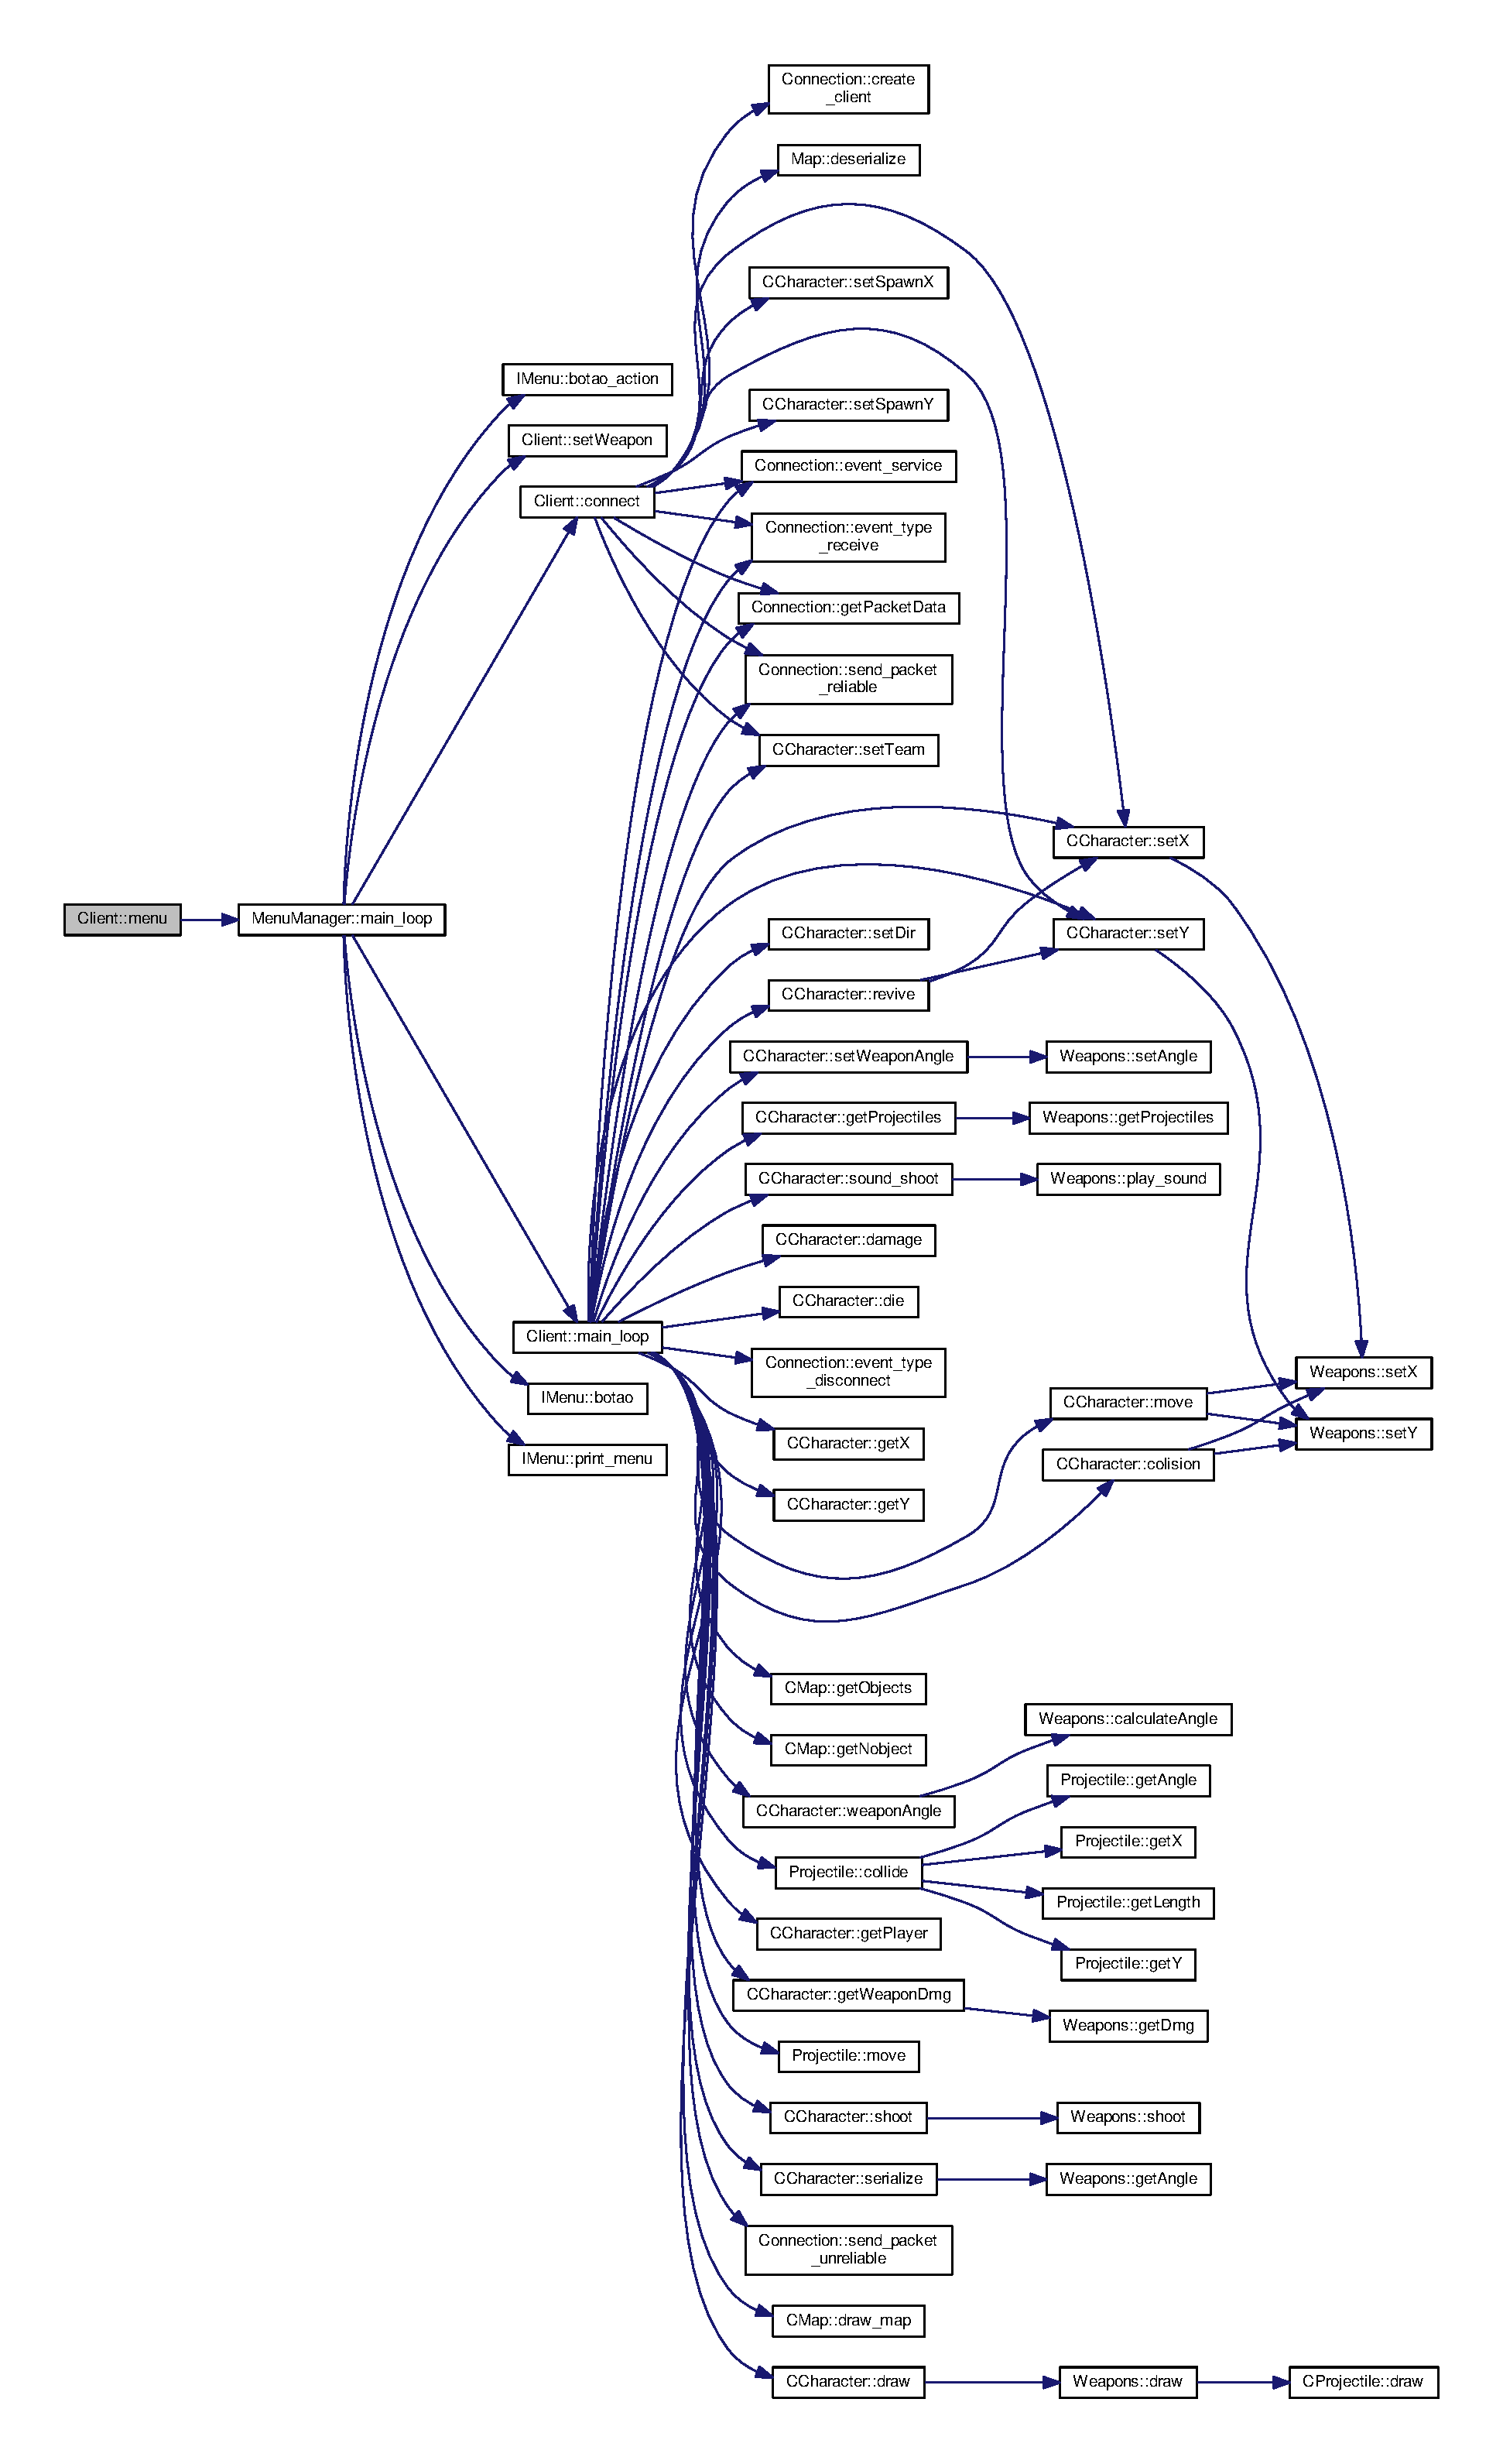
\includegraphics[height=550pt]{class_client_a8a2de145bff51cff643e5a8d773d35fe_cgraph}
\end{center}
\end{figure}




Here is the caller graph for this function\+:\nopagebreak
\begin{figure}[H]
\begin{center}
\leavevmode
\includegraphics[width=226pt]{class_client_a8a2de145bff51cff643e5a8d773d35fe_icgraph}
\end{center}
\end{figure}


\hypertarget{class_client_ab8104db60235ae805fb77a8cb161c4b8}{}\index{Client@{Client}!set\+Weapon@{set\+Weapon}}
\index{set\+Weapon@{set\+Weapon}!Client@{Client}}
\subsubsection[{set\+Weapon(\+Weapon my\+Weapon)}]{\setlength{\rightskip}{0pt plus 5cm}void Client\+::set\+Weapon (
\begin{DoxyParamCaption}
\item[{{\bf Weapon}}]{my\+Weapon}
\end{DoxyParamCaption}
)\hspace{0.3cm}{\ttfamily [inline]}}\label{class_client_ab8104db60235ae805fb77a8cb161c4b8}


Here is the caller graph for this function\+:\nopagebreak
\begin{figure}[H]
\begin{center}
\leavevmode
\includegraphics[width=350pt]{class_client_ab8104db60235ae805fb77a8cb161c4b8_icgraph}
\end{center}
\end{figure}




The documentation for this class was generated from the following files\+:\begin{DoxyCompactItemize}
\item 
/home/clemente/projects/\+Troll-\/\+Killers/\hyperlink{_client_8hpp}{Client.\+hpp}\item 
/home/clemente/projects/\+Troll-\/\+Killers/\hyperlink{_client_8cpp}{Client.\+cpp}\end{DoxyCompactItemize}

\hypertarget{class_c_map}{}\section{C\+Map Class Reference}
\label{class_c_map}\index{C\+Map@{C\+Map}}


{\ttfamily \#include $<$C\+Map.\+hpp$>$}



Inheritance diagram for C\+Map\+:\nopagebreak
\begin{figure}[H]
\begin{center}
\leavevmode
\includegraphics[width=179pt]{class_c_map__inherit__graph}
\end{center}
\end{figure}


Collaboration diagram for C\+Map\+:\nopagebreak
\begin{figure}[H]
\begin{center}
\leavevmode
\includegraphics[height=550pt]{class_c_map__coll__graph}
\end{center}
\end{figure}
\subsection*{Public Member Functions}
\begin{DoxyCompactItemize}
\item 
\hyperlink{class_c_map_a57a9b9c9b6d833102dd19852ec3767de}{C\+Map} (std\+::string \hyperlink{class_map_abe0a2d1af671ad7ca47651a8d207b23c}{name}, int \hyperlink{class_map_a6cb94f4c91b4634128ccf0219f84d1ab}{max\+\_\+objects}, int \hyperlink{class_map_a48caa289073dbeff9c89a02cf89a2cc6}{length}, int \hyperlink{class_map_a15981e529cd48e04432898f9185683d3}{width})
\item 
\hyperlink{class_c_map_a7ad71523562247ed2183e57eaed018e8}{C\+Map} ()
\item 
void \hyperlink{class_c_map_abec86992ac01292170213a5d71f17895}{new\+\_\+object} (\hyperlink{struct__object}{\+\_\+object} object)
\item 
void \hyperlink{class_c_map_a9e069b9af7a4a243345dd0bfae24121a}{destroy\+\_\+object} (int x, int y)
\item 
void \hyperlink{class_c_map_adedfa138aa67c2924e79809ad1dac85c}{draw\+\_\+map} (int x, int y)
\item 
void \hyperlink{class_c_map_a6b9de17f30f934892113c02b4f53779d}{set\+Draw\+Circles} (bool draw\+Circles)
\item 
\hyperlink{struct__object}{\+\_\+object} $\ast$ \hyperlink{class_c_map_aa735d6c214fe5c973edf82f3eaa4431e}{get\+Objects} ()
\item 
int \hyperlink{class_c_map_a1b1e0a1671eb60396ce30c393173a8a2}{get\+Nobject} ()
\item 
\hyperlink{class_c_map_a9419f5696c22e9569612b79db2872e02}{$\sim$\+C\+Map} ()
\end{DoxyCompactItemize}
\subsection*{Additional Inherited Members}


\subsection{Constructor \& Destructor Documentation}
\hypertarget{class_c_map_a57a9b9c9b6d833102dd19852ec3767de}{}\index{C\+Map@{C\+Map}!C\+Map@{C\+Map}}
\index{C\+Map@{C\+Map}!C\+Map@{C\+Map}}
\subsubsection[{C\+Map(std\+::string name, int max\+\_\+objects, int length, int width)}]{\setlength{\rightskip}{0pt plus 5cm}C\+Map\+::\+C\+Map (
\begin{DoxyParamCaption}
\item[{std\+::string}]{name, }
\item[{int}]{max\+\_\+objects, }
\item[{int}]{length, }
\item[{int}]{width}
\end{DoxyParamCaption}
)}\label{class_c_map_a57a9b9c9b6d833102dd19852ec3767de}
\hypertarget{class_c_map_a7ad71523562247ed2183e57eaed018e8}{}\index{C\+Map@{C\+Map}!C\+Map@{C\+Map}}
\index{C\+Map@{C\+Map}!C\+Map@{C\+Map}}
\subsubsection[{C\+Map()}]{\setlength{\rightskip}{0pt plus 5cm}C\+Map\+::\+C\+Map (
\begin{DoxyParamCaption}
{}
\end{DoxyParamCaption}
)}\label{class_c_map_a7ad71523562247ed2183e57eaed018e8}
\hypertarget{class_c_map_a9419f5696c22e9569612b79db2872e02}{}\index{C\+Map@{C\+Map}!````~C\+Map@{$\sim$\+C\+Map}}
\index{````~C\+Map@{$\sim$\+C\+Map}!C\+Map@{C\+Map}}
\subsubsection[{$\sim$\+C\+Map()}]{\setlength{\rightskip}{0pt plus 5cm}C\+Map\+::$\sim$\+C\+Map (
\begin{DoxyParamCaption}
{}
\end{DoxyParamCaption}
)}\label{class_c_map_a9419f5696c22e9569612b79db2872e02}


\subsection{Member Function Documentation}
\hypertarget{class_c_map_a9e069b9af7a4a243345dd0bfae24121a}{}\index{C\+Map@{C\+Map}!destroy\+\_\+object@{destroy\+\_\+object}}
\index{destroy\+\_\+object@{destroy\+\_\+object}!C\+Map@{C\+Map}}
\subsubsection[{destroy\+\_\+object(int x, int y)}]{\setlength{\rightskip}{0pt plus 5cm}void C\+Map\+::destroy\+\_\+object (
\begin{DoxyParamCaption}
\item[{int}]{x, }
\item[{int}]{y}
\end{DoxyParamCaption}
)}\label{class_c_map_a9e069b9af7a4a243345dd0bfae24121a}


Here is the caller graph for this function\+:\nopagebreak
\begin{figure}[H]
\begin{center}
\leavevmode
\includegraphics[width=350pt]{class_c_map_a9e069b9af7a4a243345dd0bfae24121a_icgraph}
\end{center}
\end{figure}


\hypertarget{class_c_map_adedfa138aa67c2924e79809ad1dac85c}{}\index{C\+Map@{C\+Map}!draw\+\_\+map@{draw\+\_\+map}}
\index{draw\+\_\+map@{draw\+\_\+map}!C\+Map@{C\+Map}}
\subsubsection[{draw\+\_\+map(int x, int y)}]{\setlength{\rightskip}{0pt plus 5cm}void C\+Map\+::draw\+\_\+map (
\begin{DoxyParamCaption}
\item[{int}]{x, }
\item[{int}]{y}
\end{DoxyParamCaption}
)}\label{class_c_map_adedfa138aa67c2924e79809ad1dac85c}


Here is the caller graph for this function\+:\nopagebreak
\begin{figure}[H]
\begin{center}
\leavevmode
\includegraphics[width=350pt]{class_c_map_adedfa138aa67c2924e79809ad1dac85c_icgraph}
\end{center}
\end{figure}


\hypertarget{class_c_map_a1b1e0a1671eb60396ce30c393173a8a2}{}\index{C\+Map@{C\+Map}!get\+Nobject@{get\+Nobject}}
\index{get\+Nobject@{get\+Nobject}!C\+Map@{C\+Map}}
\subsubsection[{get\+Nobject()}]{\setlength{\rightskip}{0pt plus 5cm}int C\+Map\+::get\+Nobject (
\begin{DoxyParamCaption}
{}
\end{DoxyParamCaption}
)\hspace{0.3cm}{\ttfamily [inline]}}\label{class_c_map_a1b1e0a1671eb60396ce30c393173a8a2}


Here is the caller graph for this function\+:\nopagebreak
\begin{figure}[H]
\begin{center}
\leavevmode
\includegraphics[width=350pt]{class_c_map_a1b1e0a1671eb60396ce30c393173a8a2_icgraph}
\end{center}
\end{figure}


\hypertarget{class_c_map_aa735d6c214fe5c973edf82f3eaa4431e}{}\index{C\+Map@{C\+Map}!get\+Objects@{get\+Objects}}
\index{get\+Objects@{get\+Objects}!C\+Map@{C\+Map}}
\subsubsection[{get\+Objects()}]{\setlength{\rightskip}{0pt plus 5cm}{\bf \+\_\+object}$\ast$ C\+Map\+::get\+Objects (
\begin{DoxyParamCaption}
{}
\end{DoxyParamCaption}
)\hspace{0.3cm}{\ttfamily [inline]}}\label{class_c_map_aa735d6c214fe5c973edf82f3eaa4431e}


Here is the caller graph for this function\+:\nopagebreak
\begin{figure}[H]
\begin{center}
\leavevmode
\includegraphics[width=350pt]{class_c_map_aa735d6c214fe5c973edf82f3eaa4431e_icgraph}
\end{center}
\end{figure}


\hypertarget{class_c_map_abec86992ac01292170213a5d71f17895}{}\index{C\+Map@{C\+Map}!new\+\_\+object@{new\+\_\+object}}
\index{new\+\_\+object@{new\+\_\+object}!C\+Map@{C\+Map}}
\subsubsection[{new\+\_\+object(\+\_\+object object)}]{\setlength{\rightskip}{0pt plus 5cm}void C\+Map\+::new\+\_\+object (
\begin{DoxyParamCaption}
\item[{{\bf \+\_\+object}}]{object}
\end{DoxyParamCaption}
)}\label{class_c_map_abec86992ac01292170213a5d71f17895}


Here is the caller graph for this function\+:\nopagebreak
\begin{figure}[H]
\begin{center}
\leavevmode
\includegraphics[width=350pt]{class_c_map_abec86992ac01292170213a5d71f17895_icgraph}
\end{center}
\end{figure}


\hypertarget{class_c_map_a6b9de17f30f934892113c02b4f53779d}{}\index{C\+Map@{C\+Map}!set\+Draw\+Circles@{set\+Draw\+Circles}}
\index{set\+Draw\+Circles@{set\+Draw\+Circles}!C\+Map@{C\+Map}}
\subsubsection[{set\+Draw\+Circles(bool draw\+Circles)}]{\setlength{\rightskip}{0pt plus 5cm}void C\+Map\+::set\+Draw\+Circles (
\begin{DoxyParamCaption}
\item[{bool}]{draw\+Circles}
\end{DoxyParamCaption}
)\hspace{0.3cm}{\ttfamily [inline]}}\label{class_c_map_a6b9de17f30f934892113c02b4f53779d}


Here is the caller graph for this function\+:\nopagebreak
\begin{figure}[H]
\begin{center}
\leavevmode
\includegraphics[width=343pt]{class_c_map_a6b9de17f30f934892113c02b4f53779d_icgraph}
\end{center}
\end{figure}




The documentation for this class was generated from the following files\+:\begin{DoxyCompactItemize}
\item 
/home/clemente/projects/\+Troll-\/\+Killers/\hyperlink{_c_map_8hpp}{C\+Map.\+hpp}\item 
/home/clemente/projects/\+Troll-\/\+Killers/\hyperlink{_c_map_8cpp}{C\+Map.\+cpp}\end{DoxyCompactItemize}

\hypertarget{class_configuration}{}\section{Configuration Class Reference}
\label{class_configuration}\index{Configuration@{Configuration}}


{\ttfamily \#include $<$Configuration.\+hpp$>$}



Collaboration diagram for Configuration\+:\nopagebreak
\begin{figure}[H]
\begin{center}
\leavevmode
\includegraphics[width=175pt]{class_configuration__coll__graph}
\end{center}
\end{figure}
\subsection*{Public Member Functions}
\begin{DoxyCompactItemize}
\item 
\hyperlink{class_configuration_a779947337bf652f0e773cb29f37f14ba}{Configuration} ()
\item 
\hyperlink{class_configuration_a0dd0fa189e239f4c9a036303f641441e}{$\sim$\+Configuration} ()
\item 
bool \hyperlink{class_configuration_a9eb938cc99deddd6b9730ee10576b55a}{config\+\_\+found} (const char $\ast$)
\item 
bool \hyperlink{class_configuration_a19490e0e191f69330f1f3efa988ed99a}{config\+\_\+create} (const char $\ast$)
\item 
bool \hyperlink{class_configuration_aed21dbeb0bcb1de61389deee612d9074}{config\+\_\+load} (const char $\ast$)
\item 
bool \hyperlink{class_configuration_aea42a72a64052e67db46c0369d731a5e}{config\+\_\+save} ()
\item 
bool \hyperlink{class_configuration_aa73dc1019f3fe1678ff56321d2e32960}{config\+\_\+insert} (const char $\ast$, const char $\ast$)
\item 
bool \hyperlink{class_configuration_a8a66e437127dfe28d70690d53f6dfd7f}{config\+\_\+get} (char $\ast$, const char $\ast$)
\item 
bool \hyperlink{class_configuration_a971a8c8fdd4e21f63c76e21ce19d7b61}{config\+\_\+remove} (const char $\ast$)
\end{DoxyCompactItemize}


\subsection{Constructor \& Destructor Documentation}
\hypertarget{class_configuration_a779947337bf652f0e773cb29f37f14ba}{}\index{Configuration@{Configuration}!Configuration@{Configuration}}
\index{Configuration@{Configuration}!Configuration@{Configuration}}
\subsubsection[{Configuration()}]{\setlength{\rightskip}{0pt plus 5cm}Configuration\+::\+Configuration (
\begin{DoxyParamCaption}
{}
\end{DoxyParamCaption}
)}\label{class_configuration_a779947337bf652f0e773cb29f37f14ba}
\hypertarget{class_configuration_a0dd0fa189e239f4c9a036303f641441e}{}\index{Configuration@{Configuration}!````~Configuration@{$\sim$\+Configuration}}
\index{````~Configuration@{$\sim$\+Configuration}!Configuration@{Configuration}}
\subsubsection[{$\sim$\+Configuration()}]{\setlength{\rightskip}{0pt plus 5cm}Configuration\+::$\sim$\+Configuration (
\begin{DoxyParamCaption}
{}
\end{DoxyParamCaption}
)}\label{class_configuration_a0dd0fa189e239f4c9a036303f641441e}


\subsection{Member Function Documentation}
\hypertarget{class_configuration_a19490e0e191f69330f1f3efa988ed99a}{}\index{Configuration@{Configuration}!config\+\_\+create@{config\+\_\+create}}
\index{config\+\_\+create@{config\+\_\+create}!Configuration@{Configuration}}
\subsubsection[{config\+\_\+create(const char $\ast$)}]{\setlength{\rightskip}{0pt plus 5cm}bool Configuration\+::config\+\_\+create (
\begin{DoxyParamCaption}
\item[{const char $\ast$}]{file\+Name}
\end{DoxyParamCaption}
)}\label{class_configuration_a19490e0e191f69330f1f3efa988ed99a}
\hypertarget{class_configuration_a9eb938cc99deddd6b9730ee10576b55a}{}\index{Configuration@{Configuration}!config\+\_\+found@{config\+\_\+found}}
\index{config\+\_\+found@{config\+\_\+found}!Configuration@{Configuration}}
\subsubsection[{config\+\_\+found(const char $\ast$)}]{\setlength{\rightskip}{0pt plus 5cm}bool Configuration\+::config\+\_\+found (
\begin{DoxyParamCaption}
\item[{const char $\ast$}]{file\+Name}
\end{DoxyParamCaption}
)}\label{class_configuration_a9eb938cc99deddd6b9730ee10576b55a}
\hypertarget{class_configuration_a8a66e437127dfe28d70690d53f6dfd7f}{}\index{Configuration@{Configuration}!config\+\_\+get@{config\+\_\+get}}
\index{config\+\_\+get@{config\+\_\+get}!Configuration@{Configuration}}
\subsubsection[{config\+\_\+get(char $\ast$, const char $\ast$)}]{\setlength{\rightskip}{0pt plus 5cm}bool Configuration\+::config\+\_\+get (
\begin{DoxyParamCaption}
\item[{char $\ast$}]{string\+Out, }
\item[{const char $\ast$}]{config\+Tag}
\end{DoxyParamCaption}
)}\label{class_configuration_a8a66e437127dfe28d70690d53f6dfd7f}


Here is the caller graph for this function\+:\nopagebreak
\begin{figure}[H]
\begin{center}
\leavevmode
\includegraphics[width=321pt]{class_configuration_a8a66e437127dfe28d70690d53f6dfd7f_icgraph}
\end{center}
\end{figure}


\hypertarget{class_configuration_aa73dc1019f3fe1678ff56321d2e32960}{}\index{Configuration@{Configuration}!config\+\_\+insert@{config\+\_\+insert}}
\index{config\+\_\+insert@{config\+\_\+insert}!Configuration@{Configuration}}
\subsubsection[{config\+\_\+insert(const char $\ast$, const char $\ast$)}]{\setlength{\rightskip}{0pt plus 5cm}bool Configuration\+::config\+\_\+insert (
\begin{DoxyParamCaption}
\item[{const char $\ast$}]{config\+Tag, }
\item[{const char $\ast$}]{data}
\end{DoxyParamCaption}
)}\label{class_configuration_aa73dc1019f3fe1678ff56321d2e32960}
\hypertarget{class_configuration_aed21dbeb0bcb1de61389deee612d9074}{}\index{Configuration@{Configuration}!config\+\_\+load@{config\+\_\+load}}
\index{config\+\_\+load@{config\+\_\+load}!Configuration@{Configuration}}
\subsubsection[{config\+\_\+load(const char $\ast$)}]{\setlength{\rightskip}{0pt plus 5cm}bool Configuration\+::config\+\_\+load (
\begin{DoxyParamCaption}
\item[{const char $\ast$}]{file\+Name}
\end{DoxyParamCaption}
)}\label{class_configuration_aed21dbeb0bcb1de61389deee612d9074}


Here is the caller graph for this function\+:\nopagebreak
\begin{figure}[H]
\begin{center}
\leavevmode
\includegraphics[width=326pt]{class_configuration_aed21dbeb0bcb1de61389deee612d9074_icgraph}
\end{center}
\end{figure}


\hypertarget{class_configuration_a971a8c8fdd4e21f63c76e21ce19d7b61}{}\index{Configuration@{Configuration}!config\+\_\+remove@{config\+\_\+remove}}
\index{config\+\_\+remove@{config\+\_\+remove}!Configuration@{Configuration}}
\subsubsection[{config\+\_\+remove(const char $\ast$)}]{\setlength{\rightskip}{0pt plus 5cm}bool Configuration\+::config\+\_\+remove (
\begin{DoxyParamCaption}
\item[{const char $\ast$}]{config\+Tag}
\end{DoxyParamCaption}
)}\label{class_configuration_a971a8c8fdd4e21f63c76e21ce19d7b61}
\hypertarget{class_configuration_aea42a72a64052e67db46c0369d731a5e}{}\index{Configuration@{Configuration}!config\+\_\+save@{config\+\_\+save}}
\index{config\+\_\+save@{config\+\_\+save}!Configuration@{Configuration}}
\subsubsection[{config\+\_\+save()}]{\setlength{\rightskip}{0pt plus 5cm}bool Configuration\+::config\+\_\+save (
\begin{DoxyParamCaption}
{}
\end{DoxyParamCaption}
)}\label{class_configuration_aea42a72a64052e67db46c0369d731a5e}


The documentation for this class was generated from the following files\+:\begin{DoxyCompactItemize}
\item 
/home/clemente/projects/\+Troll-\/\+Killers/\hyperlink{_configuration_8hpp}{Configuration.\+hpp}\item 
/home/clemente/projects/\+Troll-\/\+Killers/\hyperlink{_configuration_8cpp}{Configuration.\+cpp}\end{DoxyCompactItemize}

\hypertarget{class_connection}{}\section{Connection Class Reference}
\label{class_connection}\index{Connection@{Connection}}


{\ttfamily \#include $<$Connection.\+hpp$>$}



Collaboration diagram for Connection\+:\nopagebreak
\begin{figure}[H]
\begin{center}
\leavevmode
\includegraphics[width=214pt]{class_connection__coll__graph}
\end{center}
\end{figure}
\subsection*{Public Member Functions}
\begin{DoxyCompactItemize}
\item 
\hyperlink{class_connection_a9de94289ca6259f94ef6aeba3b134a77}{Connection} ()
\item 
\hyperlink{class_connection_a2e4352edf667bea83001569e9da8a24d}{$\sim$\+Connection} ()
\item 
void \hyperlink{class_connection_acdb1c6f1844698b2688cb611f7029d7c}{create\+\_\+server} (int port, int num\+\_\+peers)
\item 
void \hyperlink{class_connection_a3dda26c4c789d0f5e54fb50cae606022}{send\+\_\+packet\+\_\+reliable} (void $\ast$data, int size, int I\+D)
\item 
void \hyperlink{class_connection_a194e26770302ecac113375475df57e42}{send\+\_\+packet\+\_\+unreliable} (void $\ast$data, int size, int I\+D)
\item 
void \hyperlink{class_connection_a2d554f43b1e9d4a71acdd1ba297fc11b}{broadcast\+\_\+packet} (void $\ast$data, int size)
\item 
void \hyperlink{class_connection_ace9a66bd4a77270df4587df1405d4033}{send\+\_\+flush} ()
\item 
int \hyperlink{class_connection_a67a66948fd3b286a0a4faaaedb69e56e}{event\+\_\+service} (int timer)
\item 
bool \hyperlink{class_connection_a75f10c526b51675497a81e1f2c26ba9e}{event\+\_\+type\+\_\+connect} ()
\item 
bool \hyperlink{class_connection_ab0db0e5c8463aca4ec668107b1a46349}{event\+\_\+type\+\_\+receive} ()
\item 
bool \hyperlink{class_connection_a58f2ca9fedd8369ebdf61725f31123ef}{event\+\_\+type\+\_\+disconnect} ()
\item 
bool \hyperlink{class_connection_a8e9748ced0d65d12e5781ef21b1e7928}{create\+\_\+client} (std\+::string ip, int port)
\item 
E\+Net\+Address \hyperlink{class_connection_a4eec19a6b526fafaf4fa87a433a0a2d4}{get\+Last\+Connection} ()
\item 
unsigned int \hyperlink{class_connection_ab1a9ae7a0dea88ea63ea4a2d1cbec4d9}{get\+Packet\+Length} ()
\item 
void $\ast$ \hyperlink{class_connection_a2431e1403029cf660aa897eba8ec978a}{get\+Packet\+Data} ()
\item 
int \hyperlink{class_connection_a6a9cbc7d881550fcc0e768e3ee7bf171}{get\+Peer\+Id} ()
\end{DoxyCompactItemize}


\subsection{Constructor \& Destructor Documentation}
\hypertarget{class_connection_a9de94289ca6259f94ef6aeba3b134a77}{}\index{Connection@{Connection}!Connection@{Connection}}
\index{Connection@{Connection}!Connection@{Connection}}
\subsubsection[{Connection()}]{\setlength{\rightskip}{0pt plus 5cm}Connection\+::\+Connection (
\begin{DoxyParamCaption}
{}
\end{DoxyParamCaption}
)}\label{class_connection_a9de94289ca6259f94ef6aeba3b134a77}
\hypertarget{class_connection_a2e4352edf667bea83001569e9da8a24d}{}\index{Connection@{Connection}!````~Connection@{$\sim$\+Connection}}
\index{````~Connection@{$\sim$\+Connection}!Connection@{Connection}}
\subsubsection[{$\sim$\+Connection()}]{\setlength{\rightskip}{0pt plus 5cm}Connection\+::$\sim$\+Connection (
\begin{DoxyParamCaption}
{}
\end{DoxyParamCaption}
)}\label{class_connection_a2e4352edf667bea83001569e9da8a24d}


\subsection{Member Function Documentation}
\hypertarget{class_connection_a2d554f43b1e9d4a71acdd1ba297fc11b}{}\index{Connection@{Connection}!broadcast\+\_\+packet@{broadcast\+\_\+packet}}
\index{broadcast\+\_\+packet@{broadcast\+\_\+packet}!Connection@{Connection}}
\subsubsection[{broadcast\+\_\+packet(void $\ast$data, int size)}]{\setlength{\rightskip}{0pt plus 5cm}void Connection\+::broadcast\+\_\+packet (
\begin{DoxyParamCaption}
\item[{void $\ast$}]{data, }
\item[{int}]{size}
\end{DoxyParamCaption}
)}\label{class_connection_a2d554f43b1e9d4a71acdd1ba297fc11b}


Here is the caller graph for this function\+:\nopagebreak
\begin{figure}[H]
\begin{center}
\leavevmode
\includegraphics[width=350pt]{class_connection_a2d554f43b1e9d4a71acdd1ba297fc11b_icgraph}
\end{center}
\end{figure}


\hypertarget{class_connection_a8e9748ced0d65d12e5781ef21b1e7928}{}\index{Connection@{Connection}!create\+\_\+client@{create\+\_\+client}}
\index{create\+\_\+client@{create\+\_\+client}!Connection@{Connection}}
\subsubsection[{create\+\_\+client(std\+::string ip, int port)}]{\setlength{\rightskip}{0pt plus 5cm}bool Connection\+::create\+\_\+client (
\begin{DoxyParamCaption}
\item[{std\+::string}]{ip, }
\item[{int}]{port}
\end{DoxyParamCaption}
)}\label{class_connection_a8e9748ced0d65d12e5781ef21b1e7928}


Here is the caller graph for this function\+:\nopagebreak
\begin{figure}[H]
\begin{center}
\leavevmode
\includegraphics[width=350pt]{class_connection_a8e9748ced0d65d12e5781ef21b1e7928_icgraph}
\end{center}
\end{figure}


\hypertarget{class_connection_acdb1c6f1844698b2688cb611f7029d7c}{}\index{Connection@{Connection}!create\+\_\+server@{create\+\_\+server}}
\index{create\+\_\+server@{create\+\_\+server}!Connection@{Connection}}
\subsubsection[{create\+\_\+server(int port, int num\+\_\+peers)}]{\setlength{\rightskip}{0pt plus 5cm}void Connection\+::create\+\_\+server (
\begin{DoxyParamCaption}
\item[{int}]{port, }
\item[{int}]{num\+\_\+peers}
\end{DoxyParamCaption}
)}\label{class_connection_acdb1c6f1844698b2688cb611f7029d7c}


Here is the caller graph for this function\+:\nopagebreak
\begin{figure}[H]
\begin{center}
\leavevmode
\includegraphics[width=295pt]{class_connection_acdb1c6f1844698b2688cb611f7029d7c_icgraph}
\end{center}
\end{figure}


\hypertarget{class_connection_a67a66948fd3b286a0a4faaaedb69e56e}{}\index{Connection@{Connection}!event\+\_\+service@{event\+\_\+service}}
\index{event\+\_\+service@{event\+\_\+service}!Connection@{Connection}}
\subsubsection[{event\+\_\+service(int timer)}]{\setlength{\rightskip}{0pt plus 5cm}int Connection\+::event\+\_\+service (
\begin{DoxyParamCaption}
\item[{int}]{timer}
\end{DoxyParamCaption}
)}\label{class_connection_a67a66948fd3b286a0a4faaaedb69e56e}


Here is the caller graph for this function\+:\nopagebreak
\begin{figure}[H]
\begin{center}
\leavevmode
\includegraphics[width=350pt]{class_connection_a67a66948fd3b286a0a4faaaedb69e56e_icgraph}
\end{center}
\end{figure}


\hypertarget{class_connection_a75f10c526b51675497a81e1f2c26ba9e}{}\index{Connection@{Connection}!event\+\_\+type\+\_\+connect@{event\+\_\+type\+\_\+connect}}
\index{event\+\_\+type\+\_\+connect@{event\+\_\+type\+\_\+connect}!Connection@{Connection}}
\subsubsection[{event\+\_\+type\+\_\+connect()}]{\setlength{\rightskip}{0pt plus 5cm}bool Connection\+::event\+\_\+type\+\_\+connect (
\begin{DoxyParamCaption}
{}
\end{DoxyParamCaption}
)}\label{class_connection_a75f10c526b51675497a81e1f2c26ba9e}


Here is the caller graph for this function\+:\nopagebreak
\begin{figure}[H]
\begin{center}
\leavevmode
\includegraphics[width=350pt]{class_connection_a75f10c526b51675497a81e1f2c26ba9e_icgraph}
\end{center}
\end{figure}


\hypertarget{class_connection_a58f2ca9fedd8369ebdf61725f31123ef}{}\index{Connection@{Connection}!event\+\_\+type\+\_\+disconnect@{event\+\_\+type\+\_\+disconnect}}
\index{event\+\_\+type\+\_\+disconnect@{event\+\_\+type\+\_\+disconnect}!Connection@{Connection}}
\subsubsection[{event\+\_\+type\+\_\+disconnect()}]{\setlength{\rightskip}{0pt plus 5cm}bool Connection\+::event\+\_\+type\+\_\+disconnect (
\begin{DoxyParamCaption}
{}
\end{DoxyParamCaption}
)}\label{class_connection_a58f2ca9fedd8369ebdf61725f31123ef}


Here is the caller graph for this function\+:\nopagebreak
\begin{figure}[H]
\begin{center}
\leavevmode
\includegraphics[width=350pt]{class_connection_a58f2ca9fedd8369ebdf61725f31123ef_icgraph}
\end{center}
\end{figure}


\hypertarget{class_connection_ab0db0e5c8463aca4ec668107b1a46349}{}\index{Connection@{Connection}!event\+\_\+type\+\_\+receive@{event\+\_\+type\+\_\+receive}}
\index{event\+\_\+type\+\_\+receive@{event\+\_\+type\+\_\+receive}!Connection@{Connection}}
\subsubsection[{event\+\_\+type\+\_\+receive()}]{\setlength{\rightskip}{0pt plus 5cm}bool Connection\+::event\+\_\+type\+\_\+receive (
\begin{DoxyParamCaption}
{}
\end{DoxyParamCaption}
)}\label{class_connection_ab0db0e5c8463aca4ec668107b1a46349}


Here is the caller graph for this function\+:\nopagebreak
\begin{figure}[H]
\begin{center}
\leavevmode
\includegraphics[width=350pt]{class_connection_ab0db0e5c8463aca4ec668107b1a46349_icgraph}
\end{center}
\end{figure}


\hypertarget{class_connection_a4eec19a6b526fafaf4fa87a433a0a2d4}{}\index{Connection@{Connection}!get\+Last\+Connection@{get\+Last\+Connection}}
\index{get\+Last\+Connection@{get\+Last\+Connection}!Connection@{Connection}}
\subsubsection[{get\+Last\+Connection()}]{\setlength{\rightskip}{0pt plus 5cm}E\+Net\+Address Connection\+::get\+Last\+Connection (
\begin{DoxyParamCaption}
{}
\end{DoxyParamCaption}
)\hspace{0.3cm}{\ttfamily [inline]}}\label{class_connection_a4eec19a6b526fafaf4fa87a433a0a2d4}
\hypertarget{class_connection_a2431e1403029cf660aa897eba8ec978a}{}\index{Connection@{Connection}!get\+Packet\+Data@{get\+Packet\+Data}}
\index{get\+Packet\+Data@{get\+Packet\+Data}!Connection@{Connection}}
\subsubsection[{get\+Packet\+Data()}]{\setlength{\rightskip}{0pt plus 5cm}void$\ast$ Connection\+::get\+Packet\+Data (
\begin{DoxyParamCaption}
{}
\end{DoxyParamCaption}
)\hspace{0.3cm}{\ttfamily [inline]}}\label{class_connection_a2431e1403029cf660aa897eba8ec978a}


Here is the caller graph for this function\+:\nopagebreak
\begin{figure}[H]
\begin{center}
\leavevmode
\includegraphics[width=350pt]{class_connection_a2431e1403029cf660aa897eba8ec978a_icgraph}
\end{center}
\end{figure}


\hypertarget{class_connection_ab1a9ae7a0dea88ea63ea4a2d1cbec4d9}{}\index{Connection@{Connection}!get\+Packet\+Length@{get\+Packet\+Length}}
\index{get\+Packet\+Length@{get\+Packet\+Length}!Connection@{Connection}}
\subsubsection[{get\+Packet\+Length()}]{\setlength{\rightskip}{0pt plus 5cm}unsigned int Connection\+::get\+Packet\+Length (
\begin{DoxyParamCaption}
{}
\end{DoxyParamCaption}
)\hspace{0.3cm}{\ttfamily [inline]}}\label{class_connection_ab1a9ae7a0dea88ea63ea4a2d1cbec4d9}
\hypertarget{class_connection_a6a9cbc7d881550fcc0e768e3ee7bf171}{}\index{Connection@{Connection}!get\+Peer\+Id@{get\+Peer\+Id}}
\index{get\+Peer\+Id@{get\+Peer\+Id}!Connection@{Connection}}
\subsubsection[{get\+Peer\+Id()}]{\setlength{\rightskip}{0pt plus 5cm}int Connection\+::get\+Peer\+Id (
\begin{DoxyParamCaption}
{}
\end{DoxyParamCaption}
)\hspace{0.3cm}{\ttfamily [inline]}}\label{class_connection_a6a9cbc7d881550fcc0e768e3ee7bf171}


Here is the caller graph for this function\+:\nopagebreak
\begin{figure}[H]
\begin{center}
\leavevmode
\includegraphics[width=350pt]{class_connection_a6a9cbc7d881550fcc0e768e3ee7bf171_icgraph}
\end{center}
\end{figure}


\hypertarget{class_connection_ace9a66bd4a77270df4587df1405d4033}{}\index{Connection@{Connection}!send\+\_\+flush@{send\+\_\+flush}}
\index{send\+\_\+flush@{send\+\_\+flush}!Connection@{Connection}}
\subsubsection[{send\+\_\+flush()}]{\setlength{\rightskip}{0pt plus 5cm}void Connection\+::send\+\_\+flush (
\begin{DoxyParamCaption}
{}
\end{DoxyParamCaption}
)}\label{class_connection_ace9a66bd4a77270df4587df1405d4033}
\hypertarget{class_connection_a3dda26c4c789d0f5e54fb50cae606022}{}\index{Connection@{Connection}!send\+\_\+packet\+\_\+reliable@{send\+\_\+packet\+\_\+reliable}}
\index{send\+\_\+packet\+\_\+reliable@{send\+\_\+packet\+\_\+reliable}!Connection@{Connection}}
\subsubsection[{send\+\_\+packet\+\_\+reliable(void $\ast$data, int size, int I\+D)}]{\setlength{\rightskip}{0pt plus 5cm}void Connection\+::send\+\_\+packet\+\_\+reliable (
\begin{DoxyParamCaption}
\item[{void $\ast$}]{data, }
\item[{int}]{size, }
\item[{int}]{I\+D}
\end{DoxyParamCaption}
)}\label{class_connection_a3dda26c4c789d0f5e54fb50cae606022}


Here is the caller graph for this function\+:\nopagebreak
\begin{figure}[H]
\begin{center}
\leavevmode
\includegraphics[width=350pt]{class_connection_a3dda26c4c789d0f5e54fb50cae606022_icgraph}
\end{center}
\end{figure}


\hypertarget{class_connection_a194e26770302ecac113375475df57e42}{}\index{Connection@{Connection}!send\+\_\+packet\+\_\+unreliable@{send\+\_\+packet\+\_\+unreliable}}
\index{send\+\_\+packet\+\_\+unreliable@{send\+\_\+packet\+\_\+unreliable}!Connection@{Connection}}
\subsubsection[{send\+\_\+packet\+\_\+unreliable(void $\ast$data, int size, int I\+D)}]{\setlength{\rightskip}{0pt plus 5cm}void Connection\+::send\+\_\+packet\+\_\+unreliable (
\begin{DoxyParamCaption}
\item[{void $\ast$}]{data, }
\item[{int}]{size, }
\item[{int}]{I\+D}
\end{DoxyParamCaption}
)}\label{class_connection_a194e26770302ecac113375475df57e42}


Here is the caller graph for this function\+:\nopagebreak
\begin{figure}[H]
\begin{center}
\leavevmode
\includegraphics[width=350pt]{class_connection_a194e26770302ecac113375475df57e42_icgraph}
\end{center}
\end{figure}




The documentation for this class was generated from the following files\+:\begin{DoxyCompactItemize}
\item 
/home/clemente/projects/\+Troll-\/\+Killers/\hyperlink{_connection_8hpp}{Connection.\+hpp}\item 
/home/clemente/projects/\+Troll-\/\+Killers/\hyperlink{_connection_8cpp}{Connection.\+cpp}\end{DoxyCompactItemize}

\hypertarget{class_c_projectile}{}\section{C\+Projectile Class Reference}
\label{class_c_projectile}\index{C\+Projectile@{C\+Projectile}}


{\ttfamily \#include $<$C\+Projectile.\+hpp$>$}



Inheritance diagram for C\+Projectile\+:\nopagebreak
\begin{figure}[H]
\begin{center}
\leavevmode
\includegraphics[height=550pt]{class_c_projectile__inherit__graph}
\end{center}
\end{figure}


Collaboration diagram for C\+Projectile\+:\nopagebreak
\begin{figure}[H]
\begin{center}
\leavevmode
\includegraphics[height=550pt]{class_c_projectile__coll__graph}
\end{center}
\end{figure}
\subsection*{Public Member Functions}
\begin{DoxyCompactItemize}
\item 
\hyperlink{class_c_projectile_af1fb343501445d3353584cb78545c7e0}{C\+Projectile} (int16\+\_\+t \hyperlink{class_projectile_a706363cbafcbe19aa68853b2821e63b5}{x}, int16\+\_\+t \hyperlink{class_projectile_a19d3eab0725a2679d39c6d316e3681ca}{y}, int16\+\_\+t \hyperlink{class_projectile_a123f18a0665fd6ae48dcbd900647defb}{length}, int16\+\_\+t \hyperlink{class_projectile_a0f40006b298e765555e5494f3bbdc929}{velocity}, float \hyperlink{class_projectile_a5c3f2c4e44bd0607dbdb55ebfb86f88b}{angle})
\item 
void \hyperlink{class_c_projectile_a164f1820536f396cc7118c0ab9bec69f}{draw} (int map\+X, int map\+Y)
\end{DoxyCompactItemize}
\subsection*{Additional Inherited Members}


\subsection{Constructor \& Destructor Documentation}
\hypertarget{class_c_projectile_af1fb343501445d3353584cb78545c7e0}{}\index{C\+Projectile@{C\+Projectile}!C\+Projectile@{C\+Projectile}}
\index{C\+Projectile@{C\+Projectile}!C\+Projectile@{C\+Projectile}}
\subsubsection[{C\+Projectile(int16\+\_\+t x, int16\+\_\+t y, int16\+\_\+t length, int16\+\_\+t velocity, float angle)}]{\setlength{\rightskip}{0pt plus 5cm}C\+Projectile\+::\+C\+Projectile (
\begin{DoxyParamCaption}
\item[{int16\+\_\+t}]{x, }
\item[{int16\+\_\+t}]{y, }
\item[{int16\+\_\+t}]{length, }
\item[{int16\+\_\+t}]{velocity, }
\item[{float}]{angle}
\end{DoxyParamCaption}
)}\label{class_c_projectile_af1fb343501445d3353584cb78545c7e0}


\subsection{Member Function Documentation}
\hypertarget{class_c_projectile_a164f1820536f396cc7118c0ab9bec69f}{}\index{C\+Projectile@{C\+Projectile}!draw@{draw}}
\index{draw@{draw}!C\+Projectile@{C\+Projectile}}
\subsubsection[{draw(int map\+X, int map\+Y)}]{\setlength{\rightskip}{0pt plus 5cm}void C\+Projectile\+::draw (
\begin{DoxyParamCaption}
\item[{int}]{map\+X, }
\item[{int}]{map\+Y}
\end{DoxyParamCaption}
)}\label{class_c_projectile_a164f1820536f396cc7118c0ab9bec69f}


Here is the caller graph for this function\+:\nopagebreak
\begin{figure}[H]
\begin{center}
\leavevmode
\includegraphics[width=350pt]{class_c_projectile_a164f1820536f396cc7118c0ab9bec69f_icgraph}
\end{center}
\end{figure}




The documentation for this class was generated from the following files\+:\begin{DoxyCompactItemize}
\item 
/home/clemente/projects/\+Troll-\/\+Killers/\hyperlink{_c_projectile_8hpp}{C\+Projectile.\+hpp}\item 
/home/clemente/projects/\+Troll-\/\+Killers/\hyperlink{_c_projectile_8cpp}{C\+Projectile.\+cpp}\end{DoxyCompactItemize}

\hypertarget{class_cursor}{}\section{Cursor Class Reference}
\label{class_cursor}\index{Cursor@{Cursor}}


{\ttfamily \#include $<$Cursor.\+hpp$>$}



Collaboration diagram for Cursor\+:\nopagebreak
\begin{figure}[H]
\begin{center}
\leavevmode
\includegraphics[width=180pt]{class_cursor__coll__graph}
\end{center}
\end{figure}
\subsection*{Public Member Functions}
\begin{DoxyCompactItemize}
\item 
\hyperlink{class_cursor_a3cbfae4aa46ddd61a5a8569566899cc2}{Cursor} (int x, int y, int res\+X, int res\+Y, int timer)
\item 
void \hyperlink{class_cursor_a5621772fb10182e95f88d7227f670de4}{draw\+\_\+cursor} ()
\item 
void \hyperlink{class_cursor_a475f603c81c80a68499051bc224e7bb8}{move\+\_\+cursor} (A\+L\+L\+E\+G\+R\+O\+\_\+\+K\+E\+Y\+B\+O\+A\+R\+D\+\_\+\+S\+T\+A\+T\+E key\+State)
\item 
int \hyperlink{class_cursor_a32172f293dc42c6256ea95241ac1f1b6}{get\+X} ()
\item 
int \hyperlink{class_cursor_a737cccaafed3d0a03977b9c5f4cfe7cf}{get\+Y} ()
\item 
void \hyperlink{class_cursor_a3f54d9a590dfb9fca1bd390b8a9c7e54}{set\+X} (int x)
\item 
void \hyperlink{class_cursor_ab2314c3d20498cb65a66f5be6c2e74d5}{set\+Y} (int y)
\item 
void \hyperlink{class_cursor_adc6a92102e4c6a08473b0b2745a8ebc4}{change\+\_\+cursor} (int i)
\item 
void \hyperlink{class_cursor_a33ed388e90bb4af04e239b684f156587}{change\+\_\+team} ()
\item 
void \hyperlink{class_cursor_ac01596d8124ec0d1d92b88212ca858e5}{increase\+\_\+object} (\hyperlink{_enums_8hpp_a224b9163917ac32fc95a60d8c1eec3aa}{Direction} inc\+Dir)
\item 
\hyperlink{struct__object}{\+\_\+object} \hyperlink{class_cursor_aaaa6b8912141e20abde48531eec76bba}{get\+Object} (int map\+X, int map\+Y)
\item 
bool \hyperlink{class_cursor_a166a2e5d9dda3e7c4b1b552a019b7f41}{object\+\_\+selected} ()
\end{DoxyCompactItemize}


\subsection{Constructor \& Destructor Documentation}
\hypertarget{class_cursor_a3cbfae4aa46ddd61a5a8569566899cc2}{}\index{Cursor@{Cursor}!Cursor@{Cursor}}
\index{Cursor@{Cursor}!Cursor@{Cursor}}
\subsubsection[{Cursor(int x, int y, int res\+X, int res\+Y, int timer)}]{\setlength{\rightskip}{0pt plus 5cm}Cursor\+::\+Cursor (
\begin{DoxyParamCaption}
\item[{int}]{x, }
\item[{int}]{y, }
\item[{int}]{res\+X, }
\item[{int}]{res\+Y, }
\item[{int}]{timer}
\end{DoxyParamCaption}
)}\label{class_cursor_a3cbfae4aa46ddd61a5a8569566899cc2}


\subsection{Member Function Documentation}
\hypertarget{class_cursor_adc6a92102e4c6a08473b0b2745a8ebc4}{}\index{Cursor@{Cursor}!change\+\_\+cursor@{change\+\_\+cursor}}
\index{change\+\_\+cursor@{change\+\_\+cursor}!Cursor@{Cursor}}
\subsubsection[{change\+\_\+cursor(int i)}]{\setlength{\rightskip}{0pt plus 5cm}void Cursor\+::change\+\_\+cursor (
\begin{DoxyParamCaption}
\item[{int}]{i}
\end{DoxyParamCaption}
)}\label{class_cursor_adc6a92102e4c6a08473b0b2745a8ebc4}


Here is the caller graph for this function\+:\nopagebreak
\begin{figure}[H]
\begin{center}
\leavevmode
\includegraphics[width=350pt]{class_cursor_adc6a92102e4c6a08473b0b2745a8ebc4_icgraph}
\end{center}
\end{figure}


\hypertarget{class_cursor_a33ed388e90bb4af04e239b684f156587}{}\index{Cursor@{Cursor}!change\+\_\+team@{change\+\_\+team}}
\index{change\+\_\+team@{change\+\_\+team}!Cursor@{Cursor}}
\subsubsection[{change\+\_\+team()}]{\setlength{\rightskip}{0pt plus 5cm}void Cursor\+::change\+\_\+team (
\begin{DoxyParamCaption}
{}
\end{DoxyParamCaption}
)}\label{class_cursor_a33ed388e90bb4af04e239b684f156587}


Here is the caller graph for this function\+:\nopagebreak
\begin{figure}[H]
\begin{center}
\leavevmode
\includegraphics[width=350pt]{class_cursor_a33ed388e90bb4af04e239b684f156587_icgraph}
\end{center}
\end{figure}


\hypertarget{class_cursor_a5621772fb10182e95f88d7227f670de4}{}\index{Cursor@{Cursor}!draw\+\_\+cursor@{draw\+\_\+cursor}}
\index{draw\+\_\+cursor@{draw\+\_\+cursor}!Cursor@{Cursor}}
\subsubsection[{draw\+\_\+cursor()}]{\setlength{\rightskip}{0pt plus 5cm}void Cursor\+::draw\+\_\+cursor (
\begin{DoxyParamCaption}
{}
\end{DoxyParamCaption}
)}\label{class_cursor_a5621772fb10182e95f88d7227f670de4}


Here is the caller graph for this function\+:\nopagebreak
\begin{figure}[H]
\begin{center}
\leavevmode
\includegraphics[width=350pt]{class_cursor_a5621772fb10182e95f88d7227f670de4_icgraph}
\end{center}
\end{figure}


\hypertarget{class_cursor_aaaa6b8912141e20abde48531eec76bba}{}\index{Cursor@{Cursor}!get\+Object@{get\+Object}}
\index{get\+Object@{get\+Object}!Cursor@{Cursor}}
\subsubsection[{get\+Object(int map\+X, int map\+Y)}]{\setlength{\rightskip}{0pt plus 5cm}{\bf \+\_\+object} Cursor\+::get\+Object (
\begin{DoxyParamCaption}
\item[{int}]{map\+X, }
\item[{int}]{map\+Y}
\end{DoxyParamCaption}
)\hspace{0.3cm}{\ttfamily [inline]}}\label{class_cursor_aaaa6b8912141e20abde48531eec76bba}


Here is the caller graph for this function\+:\nopagebreak
\begin{figure}[H]
\begin{center}
\leavevmode
\includegraphics[width=350pt]{class_cursor_aaaa6b8912141e20abde48531eec76bba_icgraph}
\end{center}
\end{figure}


\hypertarget{class_cursor_a32172f293dc42c6256ea95241ac1f1b6}{}\index{Cursor@{Cursor}!get\+X@{get\+X}}
\index{get\+X@{get\+X}!Cursor@{Cursor}}
\subsubsection[{get\+X()}]{\setlength{\rightskip}{0pt plus 5cm}int Cursor\+::get\+X (
\begin{DoxyParamCaption}
{}
\end{DoxyParamCaption}
)\hspace{0.3cm}{\ttfamily [inline]}}\label{class_cursor_a32172f293dc42c6256ea95241ac1f1b6}


Here is the caller graph for this function\+:\nopagebreak
\begin{figure}[H]
\begin{center}
\leavevmode
\includegraphics[width=350pt]{class_cursor_a32172f293dc42c6256ea95241ac1f1b6_icgraph}
\end{center}
\end{figure}


\hypertarget{class_cursor_a737cccaafed3d0a03977b9c5f4cfe7cf}{}\index{Cursor@{Cursor}!get\+Y@{get\+Y}}
\index{get\+Y@{get\+Y}!Cursor@{Cursor}}
\subsubsection[{get\+Y()}]{\setlength{\rightskip}{0pt plus 5cm}int Cursor\+::get\+Y (
\begin{DoxyParamCaption}
{}
\end{DoxyParamCaption}
)\hspace{0.3cm}{\ttfamily [inline]}}\label{class_cursor_a737cccaafed3d0a03977b9c5f4cfe7cf}


Here is the caller graph for this function\+:\nopagebreak
\begin{figure}[H]
\begin{center}
\leavevmode
\includegraphics[width=350pt]{class_cursor_a737cccaafed3d0a03977b9c5f4cfe7cf_icgraph}
\end{center}
\end{figure}


\hypertarget{class_cursor_ac01596d8124ec0d1d92b88212ca858e5}{}\index{Cursor@{Cursor}!increase\+\_\+object@{increase\+\_\+object}}
\index{increase\+\_\+object@{increase\+\_\+object}!Cursor@{Cursor}}
\subsubsection[{increase\+\_\+object(\+Direction inc\+Dir)}]{\setlength{\rightskip}{0pt plus 5cm}void Cursor\+::increase\+\_\+object (
\begin{DoxyParamCaption}
\item[{{\bf Direction}}]{inc\+Dir}
\end{DoxyParamCaption}
)}\label{class_cursor_ac01596d8124ec0d1d92b88212ca858e5}


Here is the caller graph for this function\+:\nopagebreak
\begin{figure}[H]
\begin{center}
\leavevmode
\includegraphics[width=350pt]{class_cursor_ac01596d8124ec0d1d92b88212ca858e5_icgraph}
\end{center}
\end{figure}


\hypertarget{class_cursor_a475f603c81c80a68499051bc224e7bb8}{}\index{Cursor@{Cursor}!move\+\_\+cursor@{move\+\_\+cursor}}
\index{move\+\_\+cursor@{move\+\_\+cursor}!Cursor@{Cursor}}
\subsubsection[{move\+\_\+cursor(\+A\+L\+L\+E\+G\+R\+O\+\_\+\+K\+E\+Y\+B\+O\+A\+R\+D\+\_\+\+S\+T\+A\+T\+E key\+State)}]{\setlength{\rightskip}{0pt plus 5cm}void Cursor\+::move\+\_\+cursor (
\begin{DoxyParamCaption}
\item[{A\+L\+L\+E\+G\+R\+O\+\_\+\+K\+E\+Y\+B\+O\+A\+R\+D\+\_\+\+S\+T\+A\+T\+E}]{key\+State}
\end{DoxyParamCaption}
)}\label{class_cursor_a475f603c81c80a68499051bc224e7bb8}


Here is the caller graph for this function\+:\nopagebreak
\begin{figure}[H]
\begin{center}
\leavevmode
\includegraphics[width=350pt]{class_cursor_a475f603c81c80a68499051bc224e7bb8_icgraph}
\end{center}
\end{figure}


\hypertarget{class_cursor_a166a2e5d9dda3e7c4b1b552a019b7f41}{}\index{Cursor@{Cursor}!object\+\_\+selected@{object\+\_\+selected}}
\index{object\+\_\+selected@{object\+\_\+selected}!Cursor@{Cursor}}
\subsubsection[{object\+\_\+selected()}]{\setlength{\rightskip}{0pt plus 5cm}bool Cursor\+::object\+\_\+selected (
\begin{DoxyParamCaption}
{}
\end{DoxyParamCaption}
)\hspace{0.3cm}{\ttfamily [inline]}}\label{class_cursor_a166a2e5d9dda3e7c4b1b552a019b7f41}


Here is the caller graph for this function\+:\nopagebreak
\begin{figure}[H]
\begin{center}
\leavevmode
\includegraphics[width=350pt]{class_cursor_a166a2e5d9dda3e7c4b1b552a019b7f41_icgraph}
\end{center}
\end{figure}


\hypertarget{class_cursor_a3f54d9a590dfb9fca1bd390b8a9c7e54}{}\index{Cursor@{Cursor}!set\+X@{set\+X}}
\index{set\+X@{set\+X}!Cursor@{Cursor}}
\subsubsection[{set\+X(int x)}]{\setlength{\rightskip}{0pt plus 5cm}void Cursor\+::set\+X (
\begin{DoxyParamCaption}
\item[{int}]{x}
\end{DoxyParamCaption}
)\hspace{0.3cm}{\ttfamily [inline]}}\label{class_cursor_a3f54d9a590dfb9fca1bd390b8a9c7e54}


Here is the caller graph for this function\+:\nopagebreak
\begin{figure}[H]
\begin{center}
\leavevmode
\includegraphics[width=350pt]{class_cursor_a3f54d9a590dfb9fca1bd390b8a9c7e54_icgraph}
\end{center}
\end{figure}


\hypertarget{class_cursor_ab2314c3d20498cb65a66f5be6c2e74d5}{}\index{Cursor@{Cursor}!set\+Y@{set\+Y}}
\index{set\+Y@{set\+Y}!Cursor@{Cursor}}
\subsubsection[{set\+Y(int y)}]{\setlength{\rightskip}{0pt plus 5cm}void Cursor\+::set\+Y (
\begin{DoxyParamCaption}
\item[{int}]{y}
\end{DoxyParamCaption}
)\hspace{0.3cm}{\ttfamily [inline]}}\label{class_cursor_ab2314c3d20498cb65a66f5be6c2e74d5}


Here is the caller graph for this function\+:\nopagebreak
\begin{figure}[H]
\begin{center}
\leavevmode
\includegraphics[width=350pt]{class_cursor_ab2314c3d20498cb65a66f5be6c2e74d5_icgraph}
\end{center}
\end{figure}




The documentation for this class was generated from the following files\+:\begin{DoxyCompactItemize}
\item 
/home/clemente/projects/\+Troll-\/\+Killers/\hyperlink{_cursor_8hpp}{Cursor.\+hpp}\item 
/home/clemente/projects/\+Troll-\/\+Killers/\hyperlink{_cursor_8cpp}{Cursor.\+cpp}\end{DoxyCompactItemize}

\hypertarget{class_i_g_object}{}\section{I\+G\+Object Class Reference}
\label{class_i_g_object}\index{I\+G\+Object@{I\+G\+Object}}


{\ttfamily \#include $<$I\+G\+Object.\+hpp$>$}



Inheritance diagram for I\+G\+Object\+:\nopagebreak
\begin{figure}[H]
\begin{center}
\leavevmode
\includegraphics[height=550pt]{class_i_g_object__inherit__graph}
\end{center}
\end{figure}


Collaboration diagram for I\+G\+Object\+:\nopagebreak
\begin{figure}[H]
\begin{center}
\leavevmode
\includegraphics[width=160pt]{class_i_g_object__coll__graph}
\end{center}
\end{figure}
\subsection*{Public Member Functions}
\begin{DoxyCompactItemize}
\item 
virtual int16\+\_\+t \hyperlink{class_i_g_object_a40fdbe0db5e995e22996567d77bf45c6}{get\+Id} ()=0
\item 
virtual int16\+\_\+t \hyperlink{class_i_g_object_aa6ae1f7bd99277a3558a8e90d833fa7a}{get\+X} ()=0
\item 
virtual int16\+\_\+t \hyperlink{class_i_g_object_a3491bdb3a6b6ba8d66e07443a5b5951d}{get\+Y} ()=0
\item 
virtual int16\+\_\+t \hyperlink{class_i_g_object_afc8764ec832e6a60c58dace401d65b32}{get\+Velocity} ()=0
\item 
virtual void \hyperlink{class_i_g_object_a6e2dd93acb47fc77668e2571bff3481e}{serialize} (char $\ast$buffer)=0
\item 
virtual void \hyperlink{class_i_g_object_a4b810d1b4a785d7532104113ef5cf0ba}{set\+X} (int16\+\_\+t x)=0
\item 
virtual void \hyperlink{class_i_g_object_a5092ff8b79a61c3856510adb0543f229}{set\+Y} (int16\+\_\+t y)=0
\item 
virtual \hyperlink{class_i_g_object_a9e22adafd5adb2ed8dcb20a90ea6df6d}{$\sim$\+I\+G\+Object} ()
\end{DoxyCompactItemize}


\subsection{Constructor \& Destructor Documentation}
\hypertarget{class_i_g_object_a9e22adafd5adb2ed8dcb20a90ea6df6d}{}\index{I\+G\+Object@{I\+G\+Object}!````~I\+G\+Object@{$\sim$\+I\+G\+Object}}
\index{````~I\+G\+Object@{$\sim$\+I\+G\+Object}!I\+G\+Object@{I\+G\+Object}}
\subsubsection[{$\sim$\+I\+G\+Object()}]{\setlength{\rightskip}{0pt plus 5cm}virtual I\+G\+Object\+::$\sim$\+I\+G\+Object (
\begin{DoxyParamCaption}
{}
\end{DoxyParamCaption}
)\hspace{0.3cm}{\ttfamily [inline]}, {\ttfamily [virtual]}}\label{class_i_g_object_a9e22adafd5adb2ed8dcb20a90ea6df6d}


\subsection{Member Function Documentation}
\hypertarget{class_i_g_object_a40fdbe0db5e995e22996567d77bf45c6}{}\index{I\+G\+Object@{I\+G\+Object}!get\+Id@{get\+Id}}
\index{get\+Id@{get\+Id}!I\+G\+Object@{I\+G\+Object}}
\subsubsection[{get\+Id()=0}]{\setlength{\rightskip}{0pt plus 5cm}virtual int16\+\_\+t I\+G\+Object\+::get\+Id (
\begin{DoxyParamCaption}
{}
\end{DoxyParamCaption}
)\hspace{0.3cm}{\ttfamily [pure virtual]}}\label{class_i_g_object_a40fdbe0db5e995e22996567d77bf45c6}


Implemented in \hyperlink{class_c_character_a317ea948f11c20c52b4eb915cbc6fd34}{C\+Character}, \hyperlink{class_s_character_aed3654ba330a24ac0990047e56bccd32}{S\+Character}, and \hyperlink{class_projectile_a359ade45d958b4817e63fc06b25f55af}{Projectile}.

\hypertarget{class_i_g_object_afc8764ec832e6a60c58dace401d65b32}{}\index{I\+G\+Object@{I\+G\+Object}!get\+Velocity@{get\+Velocity}}
\index{get\+Velocity@{get\+Velocity}!I\+G\+Object@{I\+G\+Object}}
\subsubsection[{get\+Velocity()=0}]{\setlength{\rightskip}{0pt plus 5cm}virtual int16\+\_\+t I\+G\+Object\+::get\+Velocity (
\begin{DoxyParamCaption}
{}
\end{DoxyParamCaption}
)\hspace{0.3cm}{\ttfamily [pure virtual]}}\label{class_i_g_object_afc8764ec832e6a60c58dace401d65b32}


Implemented in \hyperlink{class_c_character_a7074f3d5a24d61766ce4d2fe354679ee}{C\+Character}, \hyperlink{class_s_character_af36a0d74ed25de0dc9e29213b46f7928}{S\+Character}, and \hyperlink{class_projectile_a0417e5c4b9fca6aae57844c57bd78fc0}{Projectile}.

\hypertarget{class_i_g_object_aa6ae1f7bd99277a3558a8e90d833fa7a}{}\index{I\+G\+Object@{I\+G\+Object}!get\+X@{get\+X}}
\index{get\+X@{get\+X}!I\+G\+Object@{I\+G\+Object}}
\subsubsection[{get\+X()=0}]{\setlength{\rightskip}{0pt plus 5cm}virtual int16\+\_\+t I\+G\+Object\+::get\+X (
\begin{DoxyParamCaption}
{}
\end{DoxyParamCaption}
)\hspace{0.3cm}{\ttfamily [pure virtual]}}\label{class_i_g_object_aa6ae1f7bd99277a3558a8e90d833fa7a}


Implemented in \hyperlink{class_c_character_a27ef2164eae8c8858de7e22b8ae2b356}{C\+Character}, \hyperlink{class_s_character_a023df9332c559507d8986facbb37dcad}{S\+Character}, and \hyperlink{class_projectile_a274d46f885207253588d74f54ddb674d}{Projectile}.

\hypertarget{class_i_g_object_a3491bdb3a6b6ba8d66e07443a5b5951d}{}\index{I\+G\+Object@{I\+G\+Object}!get\+Y@{get\+Y}}
\index{get\+Y@{get\+Y}!I\+G\+Object@{I\+G\+Object}}
\subsubsection[{get\+Y()=0}]{\setlength{\rightskip}{0pt plus 5cm}virtual int16\+\_\+t I\+G\+Object\+::get\+Y (
\begin{DoxyParamCaption}
{}
\end{DoxyParamCaption}
)\hspace{0.3cm}{\ttfamily [pure virtual]}}\label{class_i_g_object_a3491bdb3a6b6ba8d66e07443a5b5951d}


Implemented in \hyperlink{class_c_character_a39af09fa51d180f49a58ffce78c9f25b}{C\+Character}, \hyperlink{class_s_character_acbdd136e3a70a94f2f08c7158f042de6}{S\+Character}, and \hyperlink{class_projectile_a3c5e30132bd9d414514c682e447ef0de}{Projectile}.

\hypertarget{class_i_g_object_a6e2dd93acb47fc77668e2571bff3481e}{}\index{I\+G\+Object@{I\+G\+Object}!serialize@{serialize}}
\index{serialize@{serialize}!I\+G\+Object@{I\+G\+Object}}
\subsubsection[{serialize(char $\ast$buffer)=0}]{\setlength{\rightskip}{0pt plus 5cm}virtual void I\+G\+Object\+::serialize (
\begin{DoxyParamCaption}
\item[{char $\ast$}]{buffer}
\end{DoxyParamCaption}
)\hspace{0.3cm}{\ttfamily [pure virtual]}}\label{class_i_g_object_a6e2dd93acb47fc77668e2571bff3481e}


Implemented in \hyperlink{class_c_character_a2a9cb3e98cfe4c36ea292cdc38b999d8}{C\+Character}, \hyperlink{class_s_character_ab99fa7f23b8c7c9ca45d78d5e9bb8742}{S\+Character}, and \hyperlink{class_projectile_a30ea63ab82a2dc401b8145f61310a9ae}{Projectile}.

\hypertarget{class_i_g_object_a4b810d1b4a785d7532104113ef5cf0ba}{}\index{I\+G\+Object@{I\+G\+Object}!set\+X@{set\+X}}
\index{set\+X@{set\+X}!I\+G\+Object@{I\+G\+Object}}
\subsubsection[{set\+X(int16\+\_\+t x)=0}]{\setlength{\rightskip}{0pt plus 5cm}virtual void I\+G\+Object\+::set\+X (
\begin{DoxyParamCaption}
\item[{int16\+\_\+t}]{x}
\end{DoxyParamCaption}
)\hspace{0.3cm}{\ttfamily [pure virtual]}}\label{class_i_g_object_a4b810d1b4a785d7532104113ef5cf0ba}


Implemented in \hyperlink{class_c_character_a6d92d81e7bd039572e147ebe190fab6c}{C\+Character}, \hyperlink{class_s_character_a410a1a3d599fc8e91252805ce4c50f10}{S\+Character}, and \hyperlink{class_projectile_a0ed37ed97cd4b930da3f7bffbc5e3aa6}{Projectile}.

\hypertarget{class_i_g_object_a5092ff8b79a61c3856510adb0543f229}{}\index{I\+G\+Object@{I\+G\+Object}!set\+Y@{set\+Y}}
\index{set\+Y@{set\+Y}!I\+G\+Object@{I\+G\+Object}}
\subsubsection[{set\+Y(int16\+\_\+t y)=0}]{\setlength{\rightskip}{0pt plus 5cm}virtual void I\+G\+Object\+::set\+Y (
\begin{DoxyParamCaption}
\item[{int16\+\_\+t}]{y}
\end{DoxyParamCaption}
)\hspace{0.3cm}{\ttfamily [pure virtual]}}\label{class_i_g_object_a5092ff8b79a61c3856510adb0543f229}


Implemented in \hyperlink{class_c_character_a670de9c2ba79b716953a1dac2db9e4cf}{C\+Character}, \hyperlink{class_s_character_a7034f78acd75a886ecd02912b20ddcde}{S\+Character}, and \hyperlink{class_projectile_a11e50cf592b5db73cf90a1f18ec5fe1b}{Projectile}.



The documentation for this class was generated from the following file\+:\begin{DoxyCompactItemize}
\item 
/home/clemente/projects/\+Troll-\/\+Killers/\hyperlink{_i_g_object_8hpp}{I\+G\+Object.\+hpp}\end{DoxyCompactItemize}

\hypertarget{class_i_menu}{}\section{I\+Menu Class Reference}
\label{class_i_menu}\index{I\+Menu@{I\+Menu}}


{\ttfamily \#include $<$Menu.\+hpp$>$}



Inheritance diagram for I\+Menu\+:\nopagebreak
\begin{figure}[H]
\begin{center}
\leavevmode
\includegraphics[width=276pt]{class_i_menu__inherit__graph}
\end{center}
\end{figure}


Collaboration diagram for I\+Menu\+:\nopagebreak
\begin{figure}[H]
\begin{center}
\leavevmode
\includegraphics[width=167pt]{class_i_menu__coll__graph}
\end{center}
\end{figure}
\subsection*{Public Member Functions}
\begin{DoxyCompactItemize}
\item 
virtual void \hyperlink{class_i_menu_a15171c488ff899861e4c1a435bc79596}{print\+\_\+menu} ()=0
\item 
virtual \hyperlink{class_i_menu_a2e8a43e5fa1ed784d97a985eb6a07649}{$\sim$\+I\+Menu} ()
\item 
virtual void \hyperlink{class_i_menu_a492260da0be9c0e8951761547d67e79e}{botao} (A\+L\+L\+E\+G\+R\+O\+\_\+\+M\+O\+U\+S\+E\+\_\+\+S\+T\+A\+T\+E $\ast$mouse\+State)=0
\item 
virtual int \hyperlink{class_i_menu_a984d46d1c193c7552580c2d94c7f0aee}{botao\+\_\+action} ()=0
\end{DoxyCompactItemize}


\subsection{Constructor \& Destructor Documentation}
\hypertarget{class_i_menu_a2e8a43e5fa1ed784d97a985eb6a07649}{}\index{I\+Menu@{I\+Menu}!````~I\+Menu@{$\sim$\+I\+Menu}}
\index{````~I\+Menu@{$\sim$\+I\+Menu}!I\+Menu@{I\+Menu}}
\subsubsection[{$\sim$\+I\+Menu()}]{\setlength{\rightskip}{0pt plus 5cm}virtual I\+Menu\+::$\sim$\+I\+Menu (
\begin{DoxyParamCaption}
{}
\end{DoxyParamCaption}
)\hspace{0.3cm}{\ttfamily [inline]}, {\ttfamily [virtual]}}\label{class_i_menu_a2e8a43e5fa1ed784d97a985eb6a07649}


\subsection{Member Function Documentation}
\hypertarget{class_i_menu_a492260da0be9c0e8951761547d67e79e}{}\index{I\+Menu@{I\+Menu}!botao@{botao}}
\index{botao@{botao}!I\+Menu@{I\+Menu}}
\subsubsection[{botao(\+A\+L\+L\+E\+G\+R\+O\+\_\+\+M\+O\+U\+S\+E\+\_\+\+S\+T\+A\+T\+E $\ast$mouse\+State)=0}]{\setlength{\rightskip}{0pt plus 5cm}virtual void I\+Menu\+::botao (
\begin{DoxyParamCaption}
\item[{A\+L\+L\+E\+G\+R\+O\+\_\+\+M\+O\+U\+S\+E\+\_\+\+S\+T\+A\+T\+E $\ast$}]{mouse\+State}
\end{DoxyParamCaption}
)\hspace{0.3cm}{\ttfamily [pure virtual]}}\label{class_i_menu_a492260da0be9c0e8951761547d67e79e}


Implemented in \hyperlink{class_menu_armas_afc0b66c4033827b51b26127d40c17645}{Menu\+Armas}, and \hyperlink{class_menu_princ_ad6b330e90af4e4783104d987ae05895f}{Menu\+Princ}.



Here is the caller graph for this function\+:\nopagebreak
\begin{figure}[H]
\begin{center}
\leavevmode
\includegraphics[width=350pt]{class_i_menu_a492260da0be9c0e8951761547d67e79e_icgraph}
\end{center}
\end{figure}


\hypertarget{class_i_menu_a984d46d1c193c7552580c2d94c7f0aee}{}\index{I\+Menu@{I\+Menu}!botao\+\_\+action@{botao\+\_\+action}}
\index{botao\+\_\+action@{botao\+\_\+action}!I\+Menu@{I\+Menu}}
\subsubsection[{botao\+\_\+action()=0}]{\setlength{\rightskip}{0pt plus 5cm}virtual int I\+Menu\+::botao\+\_\+action (
\begin{DoxyParamCaption}
{}
\end{DoxyParamCaption}
)\hspace{0.3cm}{\ttfamily [pure virtual]}}\label{class_i_menu_a984d46d1c193c7552580c2d94c7f0aee}


Implemented in \hyperlink{class_menu_armas_a1abc753948db8a71cb6543755bb29db6}{Menu\+Armas}, and \hyperlink{class_menu_princ_a53554f00f838402761766788649037d5}{Menu\+Princ}.



Here is the caller graph for this function\+:\nopagebreak
\begin{figure}[H]
\begin{center}
\leavevmode
\includegraphics[width=350pt]{class_i_menu_a984d46d1c193c7552580c2d94c7f0aee_icgraph}
\end{center}
\end{figure}


\hypertarget{class_i_menu_a15171c488ff899861e4c1a435bc79596}{}\index{I\+Menu@{I\+Menu}!print\+\_\+menu@{print\+\_\+menu}}
\index{print\+\_\+menu@{print\+\_\+menu}!I\+Menu@{I\+Menu}}
\subsubsection[{print\+\_\+menu()=0}]{\setlength{\rightskip}{0pt plus 5cm}virtual void I\+Menu\+::print\+\_\+menu (
\begin{DoxyParamCaption}
{}
\end{DoxyParamCaption}
)\hspace{0.3cm}{\ttfamily [pure virtual]}}\label{class_i_menu_a15171c488ff899861e4c1a435bc79596}


Implemented in \hyperlink{class_menu_armas_a05bc5afc4ad1a0dd6cf35f27de53016b}{Menu\+Armas}, and \hyperlink{class_menu_princ_a4dd3850301fa43019bb64c0a79e985d1}{Menu\+Princ}.



Here is the caller graph for this function\+:\nopagebreak
\begin{figure}[H]
\begin{center}
\leavevmode
\includegraphics[width=350pt]{class_i_menu_a15171c488ff899861e4c1a435bc79596_icgraph}
\end{center}
\end{figure}




The documentation for this class was generated from the following file\+:\begin{DoxyCompactItemize}
\item 
/home/clemente/projects/\+Troll-\/\+Killers/\hyperlink{_menu_8hpp}{Menu.\+hpp}\end{DoxyCompactItemize}

\hypertarget{class_map}{}\section{Map Class Reference}
\label{class_map}\index{Map@{Map}}


{\ttfamily \#include $<$Map.\+hpp$>$}



Inheritance diagram for Map\+:\nopagebreak
\begin{figure}[H]
\begin{center}
\leavevmode
\includegraphics[width=298pt]{class_map__inherit__graph}
\end{center}
\end{figure}


Collaboration diagram for Map\+:\nopagebreak
\begin{figure}[H]
\begin{center}
\leavevmode
\includegraphics[width=160pt]{class_map__coll__graph}
\end{center}
\end{figure}
\subsection*{Public Member Functions}
\begin{DoxyCompactItemize}
\item 
\hyperlink{class_map_a0f5ad0fd4563497b4214038cbca8b582}{Map} ()
\item 
virtual bool \hyperlink{class_map_afdd22d2739acb6a6eaf8864ee090107a}{save\+\_\+map} (std\+::string pathname)
\item 
virtual bool \hyperlink{class_map_a259bb70652389b9ecf0bc76ceca656a5}{load\+\_\+map} (std\+::string pathname)
\item 
virtual int \hyperlink{class_map_ac85777e48836aa23c8c7adac7ea50ea8}{serialize} (char $\ast$buffer)
\item 
virtual void \hyperlink{class_map_a958dfc5b0956b8a4cb1ac03b0ccfdce8}{deserialize} (char $\ast$buffer)
\item 
\hyperlink{struct__object}{\+\_\+object} $\ast$ \hyperlink{class_map_a3e692a4d7e5ce0687bf4b93254714edf}{get\+Objects} ()
\item 
\hyperlink{class_map_aa403fbe09394ccf39747588f5168e3b2}{$\sim$\+Map} ()
\end{DoxyCompactItemize}
\subsection*{Protected Attributes}
\begin{DoxyCompactItemize}
\item 
int8\+\_\+t \hyperlink{class_map_a6e7ba89e3a0a05633ae7d27dd400190f}{type}
\item 
char \hyperlink{class_map_abe0a2d1af671ad7ca47651a8d207b23c}{name} \mbox{[}50\mbox{]}
\item 
\hyperlink{struct__object}{\+\_\+object} $\ast$ \hyperlink{class_map_a1028fa8db721f28473ba471ae70fde09}{objects}
\item 
int16\+\_\+t \hyperlink{class_map_a48caa289073dbeff9c89a02cf89a2cc6}{length}
\item 
int16\+\_\+t \hyperlink{class_map_a15981e529cd48e04432898f9185683d3}{width}
\item 
int16\+\_\+t \hyperlink{class_map_a6cb94f4c91b4634128ccf0219f84d1ab}{max\+\_\+objects}
\item 
int16\+\_\+t \hyperlink{class_map_ad428bf938f205ed6d1e7af2ddd09b7ce}{n\+\_\+object}
\end{DoxyCompactItemize}


\subsection{Constructor \& Destructor Documentation}
\hypertarget{class_map_a0f5ad0fd4563497b4214038cbca8b582}{}\index{Map@{Map}!Map@{Map}}
\index{Map@{Map}!Map@{Map}}
\subsubsection[{Map()}]{\setlength{\rightskip}{0pt plus 5cm}Map\+::\+Map (
\begin{DoxyParamCaption}
{}
\end{DoxyParamCaption}
)}\label{class_map_a0f5ad0fd4563497b4214038cbca8b582}
\hypertarget{class_map_aa403fbe09394ccf39747588f5168e3b2}{}\index{Map@{Map}!````~Map@{$\sim$\+Map}}
\index{````~Map@{$\sim$\+Map}!Map@{Map}}
\subsubsection[{$\sim$\+Map()}]{\setlength{\rightskip}{0pt plus 5cm}Map\+::$\sim$\+Map (
\begin{DoxyParamCaption}
{}
\end{DoxyParamCaption}
)}\label{class_map_aa403fbe09394ccf39747588f5168e3b2}


\subsection{Member Function Documentation}
\hypertarget{class_map_a958dfc5b0956b8a4cb1ac03b0ccfdce8}{}\index{Map@{Map}!deserialize@{deserialize}}
\index{deserialize@{deserialize}!Map@{Map}}
\subsubsection[{deserialize(char $\ast$buffer)}]{\setlength{\rightskip}{0pt plus 5cm}void Map\+::deserialize (
\begin{DoxyParamCaption}
\item[{char $\ast$}]{buffer}
\end{DoxyParamCaption}
)\hspace{0.3cm}{\ttfamily [virtual]}}\label{class_map_a958dfc5b0956b8a4cb1ac03b0ccfdce8}


Here is the caller graph for this function\+:\nopagebreak
\begin{figure}[H]
\begin{center}
\leavevmode
\includegraphics[width=350pt]{class_map_a958dfc5b0956b8a4cb1ac03b0ccfdce8_icgraph}
\end{center}
\end{figure}


\hypertarget{class_map_a3e692a4d7e5ce0687bf4b93254714edf}{}\index{Map@{Map}!get\+Objects@{get\+Objects}}
\index{get\+Objects@{get\+Objects}!Map@{Map}}
\subsubsection[{get\+Objects()}]{\setlength{\rightskip}{0pt plus 5cm}{\bf \+\_\+object}$\ast$ Map\+::get\+Objects (
\begin{DoxyParamCaption}
{}
\end{DoxyParamCaption}
)\hspace{0.3cm}{\ttfamily [inline]}}\label{class_map_a3e692a4d7e5ce0687bf4b93254714edf}
\hypertarget{class_map_a259bb70652389b9ecf0bc76ceca656a5}{}\index{Map@{Map}!load\+\_\+map@{load\+\_\+map}}
\index{load\+\_\+map@{load\+\_\+map}!Map@{Map}}
\subsubsection[{load\+\_\+map(std\+::string pathname)}]{\setlength{\rightskip}{0pt plus 5cm}bool Map\+::load\+\_\+map (
\begin{DoxyParamCaption}
\item[{std\+::string}]{pathname}
\end{DoxyParamCaption}
)\hspace{0.3cm}{\ttfamily [virtual]}}\label{class_map_a259bb70652389b9ecf0bc76ceca656a5}


Here is the caller graph for this function\+:\nopagebreak
\begin{figure}[H]
\begin{center}
\leavevmode
\includegraphics[width=350pt]{class_map_a259bb70652389b9ecf0bc76ceca656a5_icgraph}
\end{center}
\end{figure}


\hypertarget{class_map_afdd22d2739acb6a6eaf8864ee090107a}{}\index{Map@{Map}!save\+\_\+map@{save\+\_\+map}}
\index{save\+\_\+map@{save\+\_\+map}!Map@{Map}}
\subsubsection[{save\+\_\+map(std\+::string pathname)}]{\setlength{\rightskip}{0pt plus 5cm}bool Map\+::save\+\_\+map (
\begin{DoxyParamCaption}
\item[{std\+::string}]{pathname}
\end{DoxyParamCaption}
)\hspace{0.3cm}{\ttfamily [virtual]}}\label{class_map_afdd22d2739acb6a6eaf8864ee090107a}


Here is the caller graph for this function\+:\nopagebreak
\begin{figure}[H]
\begin{center}
\leavevmode
\includegraphics[width=350pt]{class_map_afdd22d2739acb6a6eaf8864ee090107a_icgraph}
\end{center}
\end{figure}


\hypertarget{class_map_ac85777e48836aa23c8c7adac7ea50ea8}{}\index{Map@{Map}!serialize@{serialize}}
\index{serialize@{serialize}!Map@{Map}}
\subsubsection[{serialize(char $\ast$buffer)}]{\setlength{\rightskip}{0pt plus 5cm}int Map\+::serialize (
\begin{DoxyParamCaption}
\item[{char $\ast$}]{buffer}
\end{DoxyParamCaption}
)\hspace{0.3cm}{\ttfamily [virtual]}}\label{class_map_ac85777e48836aa23c8c7adac7ea50ea8}


\subsection{Member Data Documentation}
\hypertarget{class_map_a48caa289073dbeff9c89a02cf89a2cc6}{}\index{Map@{Map}!length@{length}}
\index{length@{length}!Map@{Map}}
\subsubsection[{length}]{\setlength{\rightskip}{0pt plus 5cm}int16\+\_\+t Map\+::length\hspace{0.3cm}{\ttfamily [protected]}}\label{class_map_a48caa289073dbeff9c89a02cf89a2cc6}
\hypertarget{class_map_a6cb94f4c91b4634128ccf0219f84d1ab}{}\index{Map@{Map}!max\+\_\+objects@{max\+\_\+objects}}
\index{max\+\_\+objects@{max\+\_\+objects}!Map@{Map}}
\subsubsection[{max\+\_\+objects}]{\setlength{\rightskip}{0pt plus 5cm}int16\+\_\+t Map\+::max\+\_\+objects\hspace{0.3cm}{\ttfamily [protected]}}\label{class_map_a6cb94f4c91b4634128ccf0219f84d1ab}
\hypertarget{class_map_ad428bf938f205ed6d1e7af2ddd09b7ce}{}\index{Map@{Map}!n\+\_\+object@{n\+\_\+object}}
\index{n\+\_\+object@{n\+\_\+object}!Map@{Map}}
\subsubsection[{n\+\_\+object}]{\setlength{\rightskip}{0pt plus 5cm}int16\+\_\+t Map\+::n\+\_\+object\hspace{0.3cm}{\ttfamily [protected]}}\label{class_map_ad428bf938f205ed6d1e7af2ddd09b7ce}
\hypertarget{class_map_abe0a2d1af671ad7ca47651a8d207b23c}{}\index{Map@{Map}!name@{name}}
\index{name@{name}!Map@{Map}}
\subsubsection[{name}]{\setlength{\rightskip}{0pt plus 5cm}char Map\+::name\mbox{[}50\mbox{]}\hspace{0.3cm}{\ttfamily [protected]}}\label{class_map_abe0a2d1af671ad7ca47651a8d207b23c}
\hypertarget{class_map_a1028fa8db721f28473ba471ae70fde09}{}\index{Map@{Map}!objects@{objects}}
\index{objects@{objects}!Map@{Map}}
\subsubsection[{objects}]{\setlength{\rightskip}{0pt plus 5cm}{\bf \+\_\+object}$\ast$ Map\+::objects\hspace{0.3cm}{\ttfamily [protected]}}\label{class_map_a1028fa8db721f28473ba471ae70fde09}
\hypertarget{class_map_a6e7ba89e3a0a05633ae7d27dd400190f}{}\index{Map@{Map}!type@{type}}
\index{type@{type}!Map@{Map}}
\subsubsection[{type}]{\setlength{\rightskip}{0pt plus 5cm}int8\+\_\+t Map\+::type\hspace{0.3cm}{\ttfamily [protected]}}\label{class_map_a6e7ba89e3a0a05633ae7d27dd400190f}
\hypertarget{class_map_a15981e529cd48e04432898f9185683d3}{}\index{Map@{Map}!width@{width}}
\index{width@{width}!Map@{Map}}
\subsubsection[{width}]{\setlength{\rightskip}{0pt plus 5cm}int16\+\_\+t Map\+::width\hspace{0.3cm}{\ttfamily [protected]}}\label{class_map_a15981e529cd48e04432898f9185683d3}


The documentation for this class was generated from the following files\+:\begin{DoxyCompactItemize}
\item 
/home/clemente/projects/\+Troll-\/\+Killers/\hyperlink{_map_8hpp}{Map.\+hpp}\item 
/home/clemente/projects/\+Troll-\/\+Killers/\hyperlink{_map_8cpp}{Map.\+cpp}\end{DoxyCompactItemize}

\hypertarget{class_map_editor}{}\section{Map\+Editor Class Reference}
\label{class_map_editor}\index{Map\+Editor@{Map\+Editor}}


{\ttfamily \#include $<$Map\+Editor.\+hpp$>$}



Collaboration diagram for Map\+Editor\+:\nopagebreak
\begin{figure}[H]
\begin{center}
\leavevmode
\includegraphics[width=162pt]{class_map_editor__coll__graph}
\end{center}
\end{figure}
\subsection*{Public Member Functions}
\begin{DoxyCompactItemize}
\item 
\hyperlink{class_map_editor_a293c325d0b53afcf3924f006cdf60363}{Map\+Editor} ()
\item 
\hyperlink{class_map_editor_a46fe3ce9d636bc72461d00f4c2d6e594}{$\sim$\+Map\+Editor} ()
\item 
void \hyperlink{class_map_editor_a5937c9b49b1e342c219f8a87d8e3dd7a}{main\+\_\+loop} ()
\item 
void \hyperlink{class_map_editor_ac956a51214ea40b1423156efda3e6e11}{draw\+\_\+grid} ()
\end{DoxyCompactItemize}


\subsection{Constructor \& Destructor Documentation}
\hypertarget{class_map_editor_a293c325d0b53afcf3924f006cdf60363}{}\index{Map\+Editor@{Map\+Editor}!Map\+Editor@{Map\+Editor}}
\index{Map\+Editor@{Map\+Editor}!Map\+Editor@{Map\+Editor}}
\subsubsection[{Map\+Editor()}]{\setlength{\rightskip}{0pt plus 5cm}Map\+Editor\+::\+Map\+Editor (
\begin{DoxyParamCaption}
{}
\end{DoxyParamCaption}
)}\label{class_map_editor_a293c325d0b53afcf3924f006cdf60363}


Here is the call graph for this function\+:\nopagebreak
\begin{figure}[H]
\begin{center}
\leavevmode
\includegraphics[width=343pt]{class_map_editor_a293c325d0b53afcf3924f006cdf60363_cgraph}
\end{center}
\end{figure}


\hypertarget{class_map_editor_a46fe3ce9d636bc72461d00f4c2d6e594}{}\index{Map\+Editor@{Map\+Editor}!````~Map\+Editor@{$\sim$\+Map\+Editor}}
\index{````~Map\+Editor@{$\sim$\+Map\+Editor}!Map\+Editor@{Map\+Editor}}
\subsubsection[{$\sim$\+Map\+Editor()}]{\setlength{\rightskip}{0pt plus 5cm}Map\+Editor\+::$\sim$\+Map\+Editor (
\begin{DoxyParamCaption}
{}
\end{DoxyParamCaption}
)}\label{class_map_editor_a46fe3ce9d636bc72461d00f4c2d6e594}


\subsection{Member Function Documentation}
\hypertarget{class_map_editor_ac956a51214ea40b1423156efda3e6e11}{}\index{Map\+Editor@{Map\+Editor}!draw\+\_\+grid@{draw\+\_\+grid}}
\index{draw\+\_\+grid@{draw\+\_\+grid}!Map\+Editor@{Map\+Editor}}
\subsubsection[{draw\+\_\+grid()}]{\setlength{\rightskip}{0pt plus 5cm}void Map\+Editor\+::draw\+\_\+grid (
\begin{DoxyParamCaption}
{}
\end{DoxyParamCaption}
)}\label{class_map_editor_ac956a51214ea40b1423156efda3e6e11}


Here is the caller graph for this function\+:\nopagebreak
\begin{figure}[H]
\begin{center}
\leavevmode
\includegraphics[width=350pt]{class_map_editor_ac956a51214ea40b1423156efda3e6e11_icgraph}
\end{center}
\end{figure}


\hypertarget{class_map_editor_a5937c9b49b1e342c219f8a87d8e3dd7a}{}\index{Map\+Editor@{Map\+Editor}!main\+\_\+loop@{main\+\_\+loop}}
\index{main\+\_\+loop@{main\+\_\+loop}!Map\+Editor@{Map\+Editor}}
\subsubsection[{main\+\_\+loop()}]{\setlength{\rightskip}{0pt plus 5cm}void Map\+Editor\+::main\+\_\+loop (
\begin{DoxyParamCaption}
{}
\end{DoxyParamCaption}
)}\label{class_map_editor_a5937c9b49b1e342c219f8a87d8e3dd7a}


Here is the call graph for this function\+:\nopagebreak
\begin{figure}[H]
\begin{center}
\leavevmode
\includegraphics[height=550pt]{class_map_editor_a5937c9b49b1e342c219f8a87d8e3dd7a_cgraph}
\end{center}
\end{figure}




Here is the caller graph for this function\+:\nopagebreak
\begin{figure}[H]
\begin{center}
\leavevmode
\includegraphics[width=265pt]{class_map_editor_a5937c9b49b1e342c219f8a87d8e3dd7a_icgraph}
\end{center}
\end{figure}




The documentation for this class was generated from the following files\+:\begin{DoxyCompactItemize}
\item 
/home/clemente/projects/\+Troll-\/\+Killers/\hyperlink{_map_editor_8hpp}{Map\+Editor.\+hpp}\item 
/home/clemente/projects/\+Troll-\/\+Killers/\hyperlink{_map_editor_8cpp}{Map\+Editor.\+cpp}\end{DoxyCompactItemize}

\hypertarget{class_menu_armas}{}\section{Menu\+Armas Class Reference}
\label{class_menu_armas}\index{Menu\+Armas@{Menu\+Armas}}


{\ttfamily \#include $<$Menu.\+hpp$>$}



Inheritance diagram for Menu\+Armas\+:\nopagebreak
\begin{figure}[H]
\begin{center}
\leavevmode
\includegraphics[width=170pt]{class_menu_armas__inherit__graph}
\end{center}
\end{figure}


Collaboration diagram for Menu\+Armas\+:\nopagebreak
\begin{figure}[H]
\begin{center}
\leavevmode
\includegraphics[width=170pt]{class_menu_armas__coll__graph}
\end{center}
\end{figure}
\subsection*{Public Member Functions}
\begin{DoxyCompactItemize}
\item 
\hyperlink{class_menu_armas_ab016179c4b0421f50d67292e915968b1}{Menu\+Armas} (int res\+\_\+x, int res\+\_\+y)
\item 
virtual \hyperlink{class_menu_armas_ab467d5debe435a27f146cfd7e3b4c72f}{$\sim$\+Menu\+Armas} ()
\item 
virtual void \hyperlink{class_menu_armas_afc0b66c4033827b51b26127d40c17645}{botao} (A\+L\+L\+E\+G\+R\+O\+\_\+\+M\+O\+U\+S\+E\+\_\+\+S\+T\+A\+T\+E $\ast$mouse\+State)
\item 
virtual void \hyperlink{class_menu_armas_a05bc5afc4ad1a0dd6cf35f27de53016b}{print\+\_\+menu} ()
\item 
virtual int \hyperlink{class_menu_armas_a1abc753948db8a71cb6543755bb29db6}{botao\+\_\+action} ()
\end{DoxyCompactItemize}


\subsection{Constructor \& Destructor Documentation}
\hypertarget{class_menu_armas_ab016179c4b0421f50d67292e915968b1}{}\index{Menu\+Armas@{Menu\+Armas}!Menu\+Armas@{Menu\+Armas}}
\index{Menu\+Armas@{Menu\+Armas}!Menu\+Armas@{Menu\+Armas}}
\subsubsection[{Menu\+Armas(int res\+\_\+x, int res\+\_\+y)}]{\setlength{\rightskip}{0pt plus 5cm}Menu\+Armas\+::\+Menu\+Armas (
\begin{DoxyParamCaption}
\item[{int}]{res\+\_\+x, }
\item[{int}]{res\+\_\+y}
\end{DoxyParamCaption}
)}\label{class_menu_armas_ab016179c4b0421f50d67292e915968b1}
\hypertarget{class_menu_armas_ab467d5debe435a27f146cfd7e3b4c72f}{}\index{Menu\+Armas@{Menu\+Armas}!````~Menu\+Armas@{$\sim$\+Menu\+Armas}}
\index{````~Menu\+Armas@{$\sim$\+Menu\+Armas}!Menu\+Armas@{Menu\+Armas}}
\subsubsection[{$\sim$\+Menu\+Armas()}]{\setlength{\rightskip}{0pt plus 5cm}Menu\+Armas\+::$\sim$\+Menu\+Armas (
\begin{DoxyParamCaption}
{}
\end{DoxyParamCaption}
)\hspace{0.3cm}{\ttfamily [virtual]}}\label{class_menu_armas_ab467d5debe435a27f146cfd7e3b4c72f}


\subsection{Member Function Documentation}
\hypertarget{class_menu_armas_afc0b66c4033827b51b26127d40c17645}{}\index{Menu\+Armas@{Menu\+Armas}!botao@{botao}}
\index{botao@{botao}!Menu\+Armas@{Menu\+Armas}}
\subsubsection[{botao(\+A\+L\+L\+E\+G\+R\+O\+\_\+\+M\+O\+U\+S\+E\+\_\+\+S\+T\+A\+T\+E $\ast$mouse\+State)}]{\setlength{\rightskip}{0pt plus 5cm}void Menu\+Armas\+::botao (
\begin{DoxyParamCaption}
\item[{A\+L\+L\+E\+G\+R\+O\+\_\+\+M\+O\+U\+S\+E\+\_\+\+S\+T\+A\+T\+E $\ast$}]{mouse\+State}
\end{DoxyParamCaption}
)\hspace{0.3cm}{\ttfamily [virtual]}}\label{class_menu_armas_afc0b66c4033827b51b26127d40c17645}


Implements \hyperlink{class_i_menu_a492260da0be9c0e8951761547d67e79e}{I\+Menu}.

\hypertarget{class_menu_armas_a1abc753948db8a71cb6543755bb29db6}{}\index{Menu\+Armas@{Menu\+Armas}!botao\+\_\+action@{botao\+\_\+action}}
\index{botao\+\_\+action@{botao\+\_\+action}!Menu\+Armas@{Menu\+Armas}}
\subsubsection[{botao\+\_\+action()}]{\setlength{\rightskip}{0pt plus 5cm}int Menu\+Armas\+::botao\+\_\+action (
\begin{DoxyParamCaption}
{}
\end{DoxyParamCaption}
)\hspace{0.3cm}{\ttfamily [virtual]}}\label{class_menu_armas_a1abc753948db8a71cb6543755bb29db6}


Implements \hyperlink{class_i_menu_a984d46d1c193c7552580c2d94c7f0aee}{I\+Menu}.

\hypertarget{class_menu_armas_a05bc5afc4ad1a0dd6cf35f27de53016b}{}\index{Menu\+Armas@{Menu\+Armas}!print\+\_\+menu@{print\+\_\+menu}}
\index{print\+\_\+menu@{print\+\_\+menu}!Menu\+Armas@{Menu\+Armas}}
\subsubsection[{print\+\_\+menu()}]{\setlength{\rightskip}{0pt plus 5cm}void Menu\+Armas\+::print\+\_\+menu (
\begin{DoxyParamCaption}
{}
\end{DoxyParamCaption}
)\hspace{0.3cm}{\ttfamily [virtual]}}\label{class_menu_armas_a05bc5afc4ad1a0dd6cf35f27de53016b}


Implements \hyperlink{class_i_menu_a15171c488ff899861e4c1a435bc79596}{I\+Menu}.



The documentation for this class was generated from the following files\+:\begin{DoxyCompactItemize}
\item 
/home/clemente/projects/\+Troll-\/\+Killers/\hyperlink{_menu_8hpp}{Menu.\+hpp}\item 
/home/clemente/projects/\+Troll-\/\+Killers/\hyperlink{_menu_8cpp}{Menu.\+cpp}\end{DoxyCompactItemize}

\hypertarget{class_menu_manager}{}\section{Menu\+Manager Class Reference}
\label{class_menu_manager}\index{Menu\+Manager@{Menu\+Manager}}


{\ttfamily \#include $<$Menu\+Manager.\+hpp$>$}



Collaboration diagram for Menu\+Manager\+:\nopagebreak
\begin{figure}[H]
\begin{center}
\leavevmode
\includegraphics[width=173pt]{class_menu_manager__coll__graph}
\end{center}
\end{figure}
\subsection*{Public Member Functions}
\begin{DoxyCompactItemize}
\item 
\hyperlink{class_menu_manager_aebb773931450c858725e371da0d50b73}{Menu\+Manager} (int res\+\_\+x, int res\+\_\+y)
\item 
int \hyperlink{class_menu_manager_a86de10f125cd9be03d15dd50e381f53d}{main\+\_\+loop} (A\+L\+L\+E\+G\+R\+O\+\_\+\+T\+I\+M\+E\+R $\ast$timer, A\+L\+L\+E\+G\+R\+O\+\_\+\+E\+V\+E\+N\+T\+\_\+\+Q\+U\+E\+U\+E $\ast$event\+\_\+queue, \hyperlink{class_client}{Client} $\ast$my\+Dad)
\end{DoxyCompactItemize}


\subsection{Constructor \& Destructor Documentation}
\hypertarget{class_menu_manager_aebb773931450c858725e371da0d50b73}{}\index{Menu\+Manager@{Menu\+Manager}!Menu\+Manager@{Menu\+Manager}}
\index{Menu\+Manager@{Menu\+Manager}!Menu\+Manager@{Menu\+Manager}}
\subsubsection[{Menu\+Manager(int res\+\_\+x, int res\+\_\+y)}]{\setlength{\rightskip}{0pt plus 5cm}Menu\+Manager\+::\+Menu\+Manager (
\begin{DoxyParamCaption}
\item[{int}]{res\+\_\+x, }
\item[{int}]{res\+\_\+y}
\end{DoxyParamCaption}
)}\label{class_menu_manager_aebb773931450c858725e371da0d50b73}


\subsection{Member Function Documentation}
\hypertarget{class_menu_manager_a86de10f125cd9be03d15dd50e381f53d}{}\index{Menu\+Manager@{Menu\+Manager}!main\+\_\+loop@{main\+\_\+loop}}
\index{main\+\_\+loop@{main\+\_\+loop}!Menu\+Manager@{Menu\+Manager}}
\subsubsection[{main\+\_\+loop(\+A\+L\+L\+E\+G\+R\+O\+\_\+\+T\+I\+M\+E\+R $\ast$timer, A\+L\+L\+E\+G\+R\+O\+\_\+\+E\+V\+E\+N\+T\+\_\+\+Q\+U\+E\+U\+E $\ast$event\+\_\+queue, Client $\ast$my\+Dad)}]{\setlength{\rightskip}{0pt plus 5cm}int Menu\+Manager\+::main\+\_\+loop (
\begin{DoxyParamCaption}
\item[{A\+L\+L\+E\+G\+R\+O\+\_\+\+T\+I\+M\+E\+R $\ast$}]{timer, }
\item[{A\+L\+L\+E\+G\+R\+O\+\_\+\+E\+V\+E\+N\+T\+\_\+\+Q\+U\+E\+U\+E $\ast$}]{event\+\_\+queue, }
\item[{{\bf Client} $\ast$}]{my\+Dad}
\end{DoxyParamCaption}
)}\label{class_menu_manager_a86de10f125cd9be03d15dd50e381f53d}


Here is the call graph for this function\+:\nopagebreak
\begin{figure}[H]
\begin{center}
\leavevmode
\includegraphics[height=550pt]{class_menu_manager_a86de10f125cd9be03d15dd50e381f53d_cgraph}
\end{center}
\end{figure}




Here is the caller graph for this function\+:\nopagebreak
\begin{figure}[H]
\begin{center}
\leavevmode
\includegraphics[width=350pt]{class_menu_manager_a86de10f125cd9be03d15dd50e381f53d_icgraph}
\end{center}
\end{figure}




The documentation for this class was generated from the following files\+:\begin{DoxyCompactItemize}
\item 
/home/clemente/projects/\+Troll-\/\+Killers/\hyperlink{_menu_manager_8hpp}{Menu\+Manager.\+hpp}\item 
/home/clemente/projects/\+Troll-\/\+Killers/\hyperlink{_menu_manager_8cpp}{Menu\+Manager.\+cpp}\end{DoxyCompactItemize}

\hypertarget{class_menu_princ}{}\section{Menu\+Princ Class Reference}
\label{class_menu_princ}\index{Menu\+Princ@{Menu\+Princ}}


{\ttfamily \#include $<$Menu.\+hpp$>$}



Inheritance diagram for Menu\+Princ\+:\nopagebreak
\begin{figure}[H]
\begin{center}
\leavevmode
\includegraphics[width=167pt]{class_menu_princ__inherit__graph}
\end{center}
\end{figure}


Collaboration diagram for Menu\+Princ\+:\nopagebreak
\begin{figure}[H]
\begin{center}
\leavevmode
\includegraphics[width=167pt]{class_menu_princ__coll__graph}
\end{center}
\end{figure}
\subsection*{Public Member Functions}
\begin{DoxyCompactItemize}
\item 
\hyperlink{class_menu_princ_a88bfd033f9794676fa2ccb380d7edf9c}{Menu\+Princ} (int res\+\_\+x, int res\+\_\+y)
\item 
virtual \hyperlink{class_menu_princ_a57ac8c3362bd27feab99bcb92d54eaf5}{$\sim$\+Menu\+Princ} ()
\item 
virtual void \hyperlink{class_menu_princ_ad6b330e90af4e4783104d987ae05895f}{botao} (A\+L\+L\+E\+G\+R\+O\+\_\+\+M\+O\+U\+S\+E\+\_\+\+S\+T\+A\+T\+E $\ast$mouse\+State)
\item 
virtual void \hyperlink{class_menu_princ_a4dd3850301fa43019bb64c0a79e985d1}{print\+\_\+menu} ()
\item 
virtual int \hyperlink{class_menu_princ_a53554f00f838402761766788649037d5}{botao\+\_\+action} ()
\end{DoxyCompactItemize}


\subsection{Constructor \& Destructor Documentation}
\hypertarget{class_menu_princ_a88bfd033f9794676fa2ccb380d7edf9c}{}\index{Menu\+Princ@{Menu\+Princ}!Menu\+Princ@{Menu\+Princ}}
\index{Menu\+Princ@{Menu\+Princ}!Menu\+Princ@{Menu\+Princ}}
\subsubsection[{Menu\+Princ(int res\+\_\+x, int res\+\_\+y)}]{\setlength{\rightskip}{0pt plus 5cm}Menu\+Princ\+::\+Menu\+Princ (
\begin{DoxyParamCaption}
\item[{int}]{res\+\_\+x, }
\item[{int}]{res\+\_\+y}
\end{DoxyParamCaption}
)}\label{class_menu_princ_a88bfd033f9794676fa2ccb380d7edf9c}
\hypertarget{class_menu_princ_a57ac8c3362bd27feab99bcb92d54eaf5}{}\index{Menu\+Princ@{Menu\+Princ}!````~Menu\+Princ@{$\sim$\+Menu\+Princ}}
\index{````~Menu\+Princ@{$\sim$\+Menu\+Princ}!Menu\+Princ@{Menu\+Princ}}
\subsubsection[{$\sim$\+Menu\+Princ()}]{\setlength{\rightskip}{0pt plus 5cm}Menu\+Princ\+::$\sim$\+Menu\+Princ (
\begin{DoxyParamCaption}
{}
\end{DoxyParamCaption}
)\hspace{0.3cm}{\ttfamily [virtual]}}\label{class_menu_princ_a57ac8c3362bd27feab99bcb92d54eaf5}


\subsection{Member Function Documentation}
\hypertarget{class_menu_princ_ad6b330e90af4e4783104d987ae05895f}{}\index{Menu\+Princ@{Menu\+Princ}!botao@{botao}}
\index{botao@{botao}!Menu\+Princ@{Menu\+Princ}}
\subsubsection[{botao(\+A\+L\+L\+E\+G\+R\+O\+\_\+\+M\+O\+U\+S\+E\+\_\+\+S\+T\+A\+T\+E $\ast$mouse\+State)}]{\setlength{\rightskip}{0pt plus 5cm}void Menu\+Princ\+::botao (
\begin{DoxyParamCaption}
\item[{A\+L\+L\+E\+G\+R\+O\+\_\+\+M\+O\+U\+S\+E\+\_\+\+S\+T\+A\+T\+E $\ast$}]{mouse\+State}
\end{DoxyParamCaption}
)\hspace{0.3cm}{\ttfamily [virtual]}}\label{class_menu_princ_ad6b330e90af4e4783104d987ae05895f}


Implements \hyperlink{class_i_menu_a492260da0be9c0e8951761547d67e79e}{I\+Menu}.

\hypertarget{class_menu_princ_a53554f00f838402761766788649037d5}{}\index{Menu\+Princ@{Menu\+Princ}!botao\+\_\+action@{botao\+\_\+action}}
\index{botao\+\_\+action@{botao\+\_\+action}!Menu\+Princ@{Menu\+Princ}}
\subsubsection[{botao\+\_\+action()}]{\setlength{\rightskip}{0pt plus 5cm}int Menu\+Princ\+::botao\+\_\+action (
\begin{DoxyParamCaption}
{}
\end{DoxyParamCaption}
)\hspace{0.3cm}{\ttfamily [virtual]}}\label{class_menu_princ_a53554f00f838402761766788649037d5}


Implements \hyperlink{class_i_menu_a984d46d1c193c7552580c2d94c7f0aee}{I\+Menu}.

\hypertarget{class_menu_princ_a4dd3850301fa43019bb64c0a79e985d1}{}\index{Menu\+Princ@{Menu\+Princ}!print\+\_\+menu@{print\+\_\+menu}}
\index{print\+\_\+menu@{print\+\_\+menu}!Menu\+Princ@{Menu\+Princ}}
\subsubsection[{print\+\_\+menu()}]{\setlength{\rightskip}{0pt plus 5cm}void Menu\+Princ\+::print\+\_\+menu (
\begin{DoxyParamCaption}
{}
\end{DoxyParamCaption}
)\hspace{0.3cm}{\ttfamily [virtual]}}\label{class_menu_princ_a4dd3850301fa43019bb64c0a79e985d1}


Implements \hyperlink{class_i_menu_a15171c488ff899861e4c1a435bc79596}{I\+Menu}.



The documentation for this class was generated from the following files\+:\begin{DoxyCompactItemize}
\item 
/home/clemente/projects/\+Troll-\/\+Killers/\hyperlink{_menu_8hpp}{Menu.\+hpp}\item 
/home/clemente/projects/\+Troll-\/\+Killers/\hyperlink{_menu_8cpp}{Menu.\+cpp}\end{DoxyCompactItemize}

\hypertarget{class_pistol}{}\section{Pistol Class Reference}
\label{class_pistol}\index{Pistol@{Pistol}}


{\ttfamily \#include $<$Pistol.\+hpp$>$}



Inheritance diagram for Pistol\+:\nopagebreak
\begin{figure}[H]
\begin{center}
\leavevmode
\includegraphics[height=550pt]{class_pistol__inherit__graph}
\end{center}
\end{figure}


Collaboration diagram for Pistol\+:\nopagebreak
\begin{figure}[H]
\begin{center}
\leavevmode
\includegraphics[height=550pt]{class_pistol__coll__graph}
\end{center}
\end{figure}
\subsection*{Public Member Functions}
\begin{DoxyCompactItemize}
\item 
\hyperlink{class_pistol_a0715c5243c875aeb8d8114954a463b47}{Pistol} ()
\item 
virtual void \hyperlink{class_pistol_a0e99963f771cc143c32a0c72158e74f1}{shoot} (A\+L\+L\+E\+G\+R\+O\+\_\+\+M\+O\+U\+S\+E\+\_\+\+S\+T\+A\+T\+E \&mouse\+State, \hyperlink{class_connection}{Connection} $\ast$conn)
\end{DoxyCompactItemize}
\subsection*{Additional Inherited Members}


\subsection{Constructor \& Destructor Documentation}
\hypertarget{class_pistol_a0715c5243c875aeb8d8114954a463b47}{}\index{Pistol@{Pistol}!Pistol@{Pistol}}
\index{Pistol@{Pistol}!Pistol@{Pistol}}
\subsubsection[{Pistol()}]{\setlength{\rightskip}{0pt plus 5cm}Pistol\+::\+Pistol (
\begin{DoxyParamCaption}
{}
\end{DoxyParamCaption}
)}\label{class_pistol_a0715c5243c875aeb8d8114954a463b47}


\subsection{Member Function Documentation}
\hypertarget{class_pistol_a0e99963f771cc143c32a0c72158e74f1}{}\index{Pistol@{Pistol}!shoot@{shoot}}
\index{shoot@{shoot}!Pistol@{Pistol}}
\subsubsection[{shoot(\+A\+L\+L\+E\+G\+R\+O\+\_\+\+M\+O\+U\+S\+E\+\_\+\+S\+T\+A\+T\+E \&mouse\+State, Connection $\ast$conn)}]{\setlength{\rightskip}{0pt plus 5cm}void Pistol\+::shoot (
\begin{DoxyParamCaption}
\item[{A\+L\+L\+E\+G\+R\+O\+\_\+\+M\+O\+U\+S\+E\+\_\+\+S\+T\+A\+T\+E \&}]{mouse\+State, }
\item[{{\bf Connection} $\ast$}]{conn}
\end{DoxyParamCaption}
)\hspace{0.3cm}{\ttfamily [virtual]}}\label{class_pistol_a0e99963f771cc143c32a0c72158e74f1}


Implements \hyperlink{class_weapons_a51990dae3d666006b2154cf501758936}{Weapons}.



Here is the call graph for this function\+:\nopagebreak
\begin{figure}[H]
\begin{center}
\leavevmode
\includegraphics[width=321pt]{class_pistol_a0e99963f771cc143c32a0c72158e74f1_cgraph}
\end{center}
\end{figure}




The documentation for this class was generated from the following files\+:\begin{DoxyCompactItemize}
\item 
/home/clemente/projects/\+Troll-\/\+Killers/\hyperlink{_pistol_8hpp}{Pistol.\+hpp}\item 
/home/clemente/projects/\+Troll-\/\+Killers/\hyperlink{_pistol_8cpp}{Pistol.\+cpp}\end{DoxyCompactItemize}

\hypertarget{class_projectile}{}\section{Projectile Class Reference}
\label{class_projectile}\index{Projectile@{Projectile}}


{\ttfamily \#include $<$Projectile.\+hpp$>$}



Inheritance diagram for Projectile\+:\nopagebreak
\begin{figure}[H]
\begin{center}
\leavevmode
\includegraphics[height=550pt]{class_projectile__inherit__graph}
\end{center}
\end{figure}


Collaboration diagram for Projectile\+:\nopagebreak
\begin{figure}[H]
\begin{center}
\leavevmode
\includegraphics[width=160pt]{class_projectile__coll__graph}
\end{center}
\end{figure}
\subsection*{Public Member Functions}
\begin{DoxyCompactItemize}
\item 
\hyperlink{class_projectile_a309d73855dcfacee8421900c4f5e4411}{Projectile} (int16\+\_\+t \hyperlink{class_projectile_a706363cbafcbe19aa68853b2821e63b5}{x}, int16\+\_\+t \hyperlink{class_projectile_a19d3eab0725a2679d39c6d316e3681ca}{y}, int16\+\_\+t \hyperlink{class_projectile_a123f18a0665fd6ae48dcbd900647defb}{length}, int16\+\_\+t \hyperlink{class_projectile_a0f40006b298e765555e5494f3bbdc929}{velocity}, float \hyperlink{class_projectile_a5c3f2c4e44bd0607dbdb55ebfb86f88b}{angle})
\item 
\hyperlink{class_projectile_ac536ed2aad56af866a2078b9a85aa16d}{Projectile} ()
\item 
int16\+\_\+t \hyperlink{class_projectile_a359ade45d958b4817e63fc06b25f55af}{get\+Id} ()
\item 
int16\+\_\+t \hyperlink{class_projectile_a274d46f885207253588d74f54ddb674d}{get\+X} ()
\item 
int16\+\_\+t \hyperlink{class_projectile_a3c5e30132bd9d414514c682e447ef0de}{get\+Y} ()
\item 
float \hyperlink{class_projectile_a58707185f143d76efe3cfcec799a7ea5}{get\+Angle} ()
\item 
int16\+\_\+t \hyperlink{class_projectile_a0417e5c4b9fca6aae57844c57bd78fc0}{get\+Velocity} ()
\item 
int16\+\_\+t \hyperlink{class_projectile_aa75120b722b0078d78e9d8416c0325a7}{get\+Length} ()
\item 
void \hyperlink{class_projectile_a30ea63ab82a2dc401b8145f61310a9ae}{serialize} (char $\ast$buffer)
\item 
void \hyperlink{class_projectile_a0ed37ed97cd4b930da3f7bffbc5e3aa6}{set\+X} (int16\+\_\+t \hyperlink{class_projectile_a706363cbafcbe19aa68853b2821e63b5}{x})
\item 
void \hyperlink{class_projectile_a11e50cf592b5db73cf90a1f18ec5fe1b}{set\+Y} (int16\+\_\+t \hyperlink{class_projectile_a19d3eab0725a2679d39c6d316e3681ca}{y})
\item 
void \hyperlink{class_projectile_a5bf8e186023fb20ec8c15476c894def2}{set\+Angle} (float \hyperlink{class_projectile_a5c3f2c4e44bd0607dbdb55ebfb86f88b}{angle})
\item 
void \hyperlink{class_projectile_ac5f6d2a73c1f82f2f11ae353d251acef}{move} ()
\end{DoxyCompactItemize}
\subsection*{Static Public Member Functions}
\begin{DoxyCompactItemize}
\item 
static bool \hyperlink{class_projectile_a50744612baf1cdc972281a99f8e0ac50}{collide} (\hyperlink{class_projectile}{Projectile} $\ast$projectile, \hyperlink{struct__object}{\+\_\+object} \&object)
\end{DoxyCompactItemize}
\subsection*{Protected Attributes}
\begin{DoxyCompactItemize}
\item 
int16\+\_\+t \hyperlink{class_projectile_a0f40006b298e765555e5494f3bbdc929}{velocity}
\item 
int16\+\_\+t \hyperlink{class_projectile_a4d5668615b5f58f8c7a2b4e0bf41d493}{id}
\item 
int16\+\_\+t \hyperlink{class_projectile_a706363cbafcbe19aa68853b2821e63b5}{x}
\item 
int16\+\_\+t \hyperlink{class_projectile_a19d3eab0725a2679d39c6d316e3681ca}{y}
\item 
int16\+\_\+t \hyperlink{class_projectile_a123f18a0665fd6ae48dcbd900647defb}{length}
\item 
float \hyperlink{class_projectile_a5c3f2c4e44bd0607dbdb55ebfb86f88b}{angle}
\end{DoxyCompactItemize}


\subsection{Constructor \& Destructor Documentation}
\hypertarget{class_projectile_a309d73855dcfacee8421900c4f5e4411}{}\index{Projectile@{Projectile}!Projectile@{Projectile}}
\index{Projectile@{Projectile}!Projectile@{Projectile}}
\subsubsection[{Projectile(int16\+\_\+t x, int16\+\_\+t y, int16\+\_\+t length, int16\+\_\+t velocity, float angle)}]{\setlength{\rightskip}{0pt plus 5cm}Projectile\+::\+Projectile (
\begin{DoxyParamCaption}
\item[{int16\+\_\+t}]{x, }
\item[{int16\+\_\+t}]{y, }
\item[{int16\+\_\+t}]{length, }
\item[{int16\+\_\+t}]{velocity, }
\item[{float}]{angle}
\end{DoxyParamCaption}
)}\label{class_projectile_a309d73855dcfacee8421900c4f5e4411}
\hypertarget{class_projectile_ac536ed2aad56af866a2078b9a85aa16d}{}\index{Projectile@{Projectile}!Projectile@{Projectile}}
\index{Projectile@{Projectile}!Projectile@{Projectile}}
\subsubsection[{Projectile()}]{\setlength{\rightskip}{0pt plus 5cm}Projectile\+::\+Projectile (
\begin{DoxyParamCaption}
{}
\end{DoxyParamCaption}
)}\label{class_projectile_ac536ed2aad56af866a2078b9a85aa16d}


\subsection{Member Function Documentation}
\hypertarget{class_projectile_a50744612baf1cdc972281a99f8e0ac50}{}\index{Projectile@{Projectile}!collide@{collide}}
\index{collide@{collide}!Projectile@{Projectile}}
\subsubsection[{collide(\+Projectile $\ast$projectile, \+\_\+object \&object)}]{\setlength{\rightskip}{0pt plus 5cm}bool Projectile\+::collide (
\begin{DoxyParamCaption}
\item[{{\bf Projectile} $\ast$}]{projectile, }
\item[{{\bf \+\_\+object} \&}]{object}
\end{DoxyParamCaption}
)\hspace{0.3cm}{\ttfamily [static]}}\label{class_projectile_a50744612baf1cdc972281a99f8e0ac50}


Here is the call graph for this function\+:\nopagebreak
\begin{figure}[H]
\begin{center}
\leavevmode
\includegraphics[width=313pt]{class_projectile_a50744612baf1cdc972281a99f8e0ac50_cgraph}
\end{center}
\end{figure}




Here is the caller graph for this function\+:\nopagebreak
\begin{figure}[H]
\begin{center}
\leavevmode
\includegraphics[width=350pt]{class_projectile_a50744612baf1cdc972281a99f8e0ac50_icgraph}
\end{center}
\end{figure}


\hypertarget{class_projectile_a58707185f143d76efe3cfcec799a7ea5}{}\index{Projectile@{Projectile}!get\+Angle@{get\+Angle}}
\index{get\+Angle@{get\+Angle}!Projectile@{Projectile}}
\subsubsection[{get\+Angle()}]{\setlength{\rightskip}{0pt plus 5cm}float Projectile\+::get\+Angle (
\begin{DoxyParamCaption}
{}
\end{DoxyParamCaption}
)\hspace{0.3cm}{\ttfamily [inline]}}\label{class_projectile_a58707185f143d76efe3cfcec799a7ea5}


Here is the caller graph for this function\+:\nopagebreak
\begin{figure}[H]
\begin{center}
\leavevmode
\includegraphics[width=350pt]{class_projectile_a58707185f143d76efe3cfcec799a7ea5_icgraph}
\end{center}
\end{figure}


\hypertarget{class_projectile_a359ade45d958b4817e63fc06b25f55af}{}\index{Projectile@{Projectile}!get\+Id@{get\+Id}}
\index{get\+Id@{get\+Id}!Projectile@{Projectile}}
\subsubsection[{get\+Id()}]{\setlength{\rightskip}{0pt plus 5cm}int16\+\_\+t Projectile\+::get\+Id (
\begin{DoxyParamCaption}
{}
\end{DoxyParamCaption}
)\hspace{0.3cm}{\ttfamily [inline]}, {\ttfamily [virtual]}}\label{class_projectile_a359ade45d958b4817e63fc06b25f55af}


Implements \hyperlink{class_i_g_object_a40fdbe0db5e995e22996567d77bf45c6}{I\+G\+Object}.

\hypertarget{class_projectile_aa75120b722b0078d78e9d8416c0325a7}{}\index{Projectile@{Projectile}!get\+Length@{get\+Length}}
\index{get\+Length@{get\+Length}!Projectile@{Projectile}}
\subsubsection[{get\+Length()}]{\setlength{\rightskip}{0pt plus 5cm}int16\+\_\+t Projectile\+::get\+Length (
\begin{DoxyParamCaption}
{}
\end{DoxyParamCaption}
)\hspace{0.3cm}{\ttfamily [inline]}}\label{class_projectile_aa75120b722b0078d78e9d8416c0325a7}


Here is the caller graph for this function\+:\nopagebreak
\begin{figure}[H]
\begin{center}
\leavevmode
\includegraphics[width=350pt]{class_projectile_aa75120b722b0078d78e9d8416c0325a7_icgraph}
\end{center}
\end{figure}


\hypertarget{class_projectile_a0417e5c4b9fca6aae57844c57bd78fc0}{}\index{Projectile@{Projectile}!get\+Velocity@{get\+Velocity}}
\index{get\+Velocity@{get\+Velocity}!Projectile@{Projectile}}
\subsubsection[{get\+Velocity()}]{\setlength{\rightskip}{0pt plus 5cm}int16\+\_\+t Projectile\+::get\+Velocity (
\begin{DoxyParamCaption}
{}
\end{DoxyParamCaption}
)\hspace{0.3cm}{\ttfamily [inline]}, {\ttfamily [virtual]}}\label{class_projectile_a0417e5c4b9fca6aae57844c57bd78fc0}


Implements \hyperlink{class_i_g_object_afc8764ec832e6a60c58dace401d65b32}{I\+G\+Object}.

\hypertarget{class_projectile_a274d46f885207253588d74f54ddb674d}{}\index{Projectile@{Projectile}!get\+X@{get\+X}}
\index{get\+X@{get\+X}!Projectile@{Projectile}}
\subsubsection[{get\+X()}]{\setlength{\rightskip}{0pt plus 5cm}int16\+\_\+t Projectile\+::get\+X (
\begin{DoxyParamCaption}
{}
\end{DoxyParamCaption}
)\hspace{0.3cm}{\ttfamily [inline]}, {\ttfamily [virtual]}}\label{class_projectile_a274d46f885207253588d74f54ddb674d}


Implements \hyperlink{class_i_g_object_aa6ae1f7bd99277a3558a8e90d833fa7a}{I\+G\+Object}.



Here is the caller graph for this function\+:\nopagebreak
\begin{figure}[H]
\begin{center}
\leavevmode
\includegraphics[width=350pt]{class_projectile_a274d46f885207253588d74f54ddb674d_icgraph}
\end{center}
\end{figure}


\hypertarget{class_projectile_a3c5e30132bd9d414514c682e447ef0de}{}\index{Projectile@{Projectile}!get\+Y@{get\+Y}}
\index{get\+Y@{get\+Y}!Projectile@{Projectile}}
\subsubsection[{get\+Y()}]{\setlength{\rightskip}{0pt plus 5cm}int16\+\_\+t Projectile\+::get\+Y (
\begin{DoxyParamCaption}
{}
\end{DoxyParamCaption}
)\hspace{0.3cm}{\ttfamily [inline]}, {\ttfamily [virtual]}}\label{class_projectile_a3c5e30132bd9d414514c682e447ef0de}


Implements \hyperlink{class_i_g_object_a3491bdb3a6b6ba8d66e07443a5b5951d}{I\+G\+Object}.



Here is the caller graph for this function\+:\nopagebreak
\begin{figure}[H]
\begin{center}
\leavevmode
\includegraphics[width=350pt]{class_projectile_a3c5e30132bd9d414514c682e447ef0de_icgraph}
\end{center}
\end{figure}


\hypertarget{class_projectile_ac5f6d2a73c1f82f2f11ae353d251acef}{}\index{Projectile@{Projectile}!move@{move}}
\index{move@{move}!Projectile@{Projectile}}
\subsubsection[{move()}]{\setlength{\rightskip}{0pt plus 5cm}void Projectile\+::move (
\begin{DoxyParamCaption}
{}
\end{DoxyParamCaption}
)}\label{class_projectile_ac5f6d2a73c1f82f2f11ae353d251acef}


Here is the caller graph for this function\+:\nopagebreak
\begin{figure}[H]
\begin{center}
\leavevmode
\includegraphics[width=350pt]{class_projectile_ac5f6d2a73c1f82f2f11ae353d251acef_icgraph}
\end{center}
\end{figure}


\hypertarget{class_projectile_a30ea63ab82a2dc401b8145f61310a9ae}{}\index{Projectile@{Projectile}!serialize@{serialize}}
\index{serialize@{serialize}!Projectile@{Projectile}}
\subsubsection[{serialize(char $\ast$buffer)}]{\setlength{\rightskip}{0pt plus 5cm}void Projectile\+::serialize (
\begin{DoxyParamCaption}
\item[{char $\ast$}]{buffer}
\end{DoxyParamCaption}
)\hspace{0.3cm}{\ttfamily [virtual]}}\label{class_projectile_a30ea63ab82a2dc401b8145f61310a9ae}


Implements \hyperlink{class_i_g_object_a6e2dd93acb47fc77668e2571bff3481e}{I\+G\+Object}.

\hypertarget{class_projectile_a5bf8e186023fb20ec8c15476c894def2}{}\index{Projectile@{Projectile}!set\+Angle@{set\+Angle}}
\index{set\+Angle@{set\+Angle}!Projectile@{Projectile}}
\subsubsection[{set\+Angle(float angle)}]{\setlength{\rightskip}{0pt plus 5cm}void Projectile\+::set\+Angle (
\begin{DoxyParamCaption}
\item[{float}]{angle}
\end{DoxyParamCaption}
)\hspace{0.3cm}{\ttfamily [inline]}}\label{class_projectile_a5bf8e186023fb20ec8c15476c894def2}
\hypertarget{class_projectile_a0ed37ed97cd4b930da3f7bffbc5e3aa6}{}\index{Projectile@{Projectile}!set\+X@{set\+X}}
\index{set\+X@{set\+X}!Projectile@{Projectile}}
\subsubsection[{set\+X(int16\+\_\+t x)}]{\setlength{\rightskip}{0pt plus 5cm}void Projectile\+::set\+X (
\begin{DoxyParamCaption}
\item[{int16\+\_\+t}]{x}
\end{DoxyParamCaption}
)\hspace{0.3cm}{\ttfamily [inline]}, {\ttfamily [virtual]}}\label{class_projectile_a0ed37ed97cd4b930da3f7bffbc5e3aa6}


Implements \hyperlink{class_i_g_object_a4b810d1b4a785d7532104113ef5cf0ba}{I\+G\+Object}.

\hypertarget{class_projectile_a11e50cf592b5db73cf90a1f18ec5fe1b}{}\index{Projectile@{Projectile}!set\+Y@{set\+Y}}
\index{set\+Y@{set\+Y}!Projectile@{Projectile}}
\subsubsection[{set\+Y(int16\+\_\+t y)}]{\setlength{\rightskip}{0pt plus 5cm}void Projectile\+::set\+Y (
\begin{DoxyParamCaption}
\item[{int16\+\_\+t}]{y}
\end{DoxyParamCaption}
)\hspace{0.3cm}{\ttfamily [inline]}, {\ttfamily [virtual]}}\label{class_projectile_a11e50cf592b5db73cf90a1f18ec5fe1b}


Implements \hyperlink{class_i_g_object_a5092ff8b79a61c3856510adb0543f229}{I\+G\+Object}.



\subsection{Member Data Documentation}
\hypertarget{class_projectile_a5c3f2c4e44bd0607dbdb55ebfb86f88b}{}\index{Projectile@{Projectile}!angle@{angle}}
\index{angle@{angle}!Projectile@{Projectile}}
\subsubsection[{angle}]{\setlength{\rightskip}{0pt plus 5cm}float Projectile\+::angle\hspace{0.3cm}{\ttfamily [protected]}}\label{class_projectile_a5c3f2c4e44bd0607dbdb55ebfb86f88b}
\hypertarget{class_projectile_a4d5668615b5f58f8c7a2b4e0bf41d493}{}\index{Projectile@{Projectile}!id@{id}}
\index{id@{id}!Projectile@{Projectile}}
\subsubsection[{id}]{\setlength{\rightskip}{0pt plus 5cm}int16\+\_\+t Projectile\+::id\hspace{0.3cm}{\ttfamily [protected]}}\label{class_projectile_a4d5668615b5f58f8c7a2b4e0bf41d493}
\hypertarget{class_projectile_a123f18a0665fd6ae48dcbd900647defb}{}\index{Projectile@{Projectile}!length@{length}}
\index{length@{length}!Projectile@{Projectile}}
\subsubsection[{length}]{\setlength{\rightskip}{0pt plus 5cm}int16\+\_\+t Projectile\+::length\hspace{0.3cm}{\ttfamily [protected]}}\label{class_projectile_a123f18a0665fd6ae48dcbd900647defb}
\hypertarget{class_projectile_a0f40006b298e765555e5494f3bbdc929}{}\index{Projectile@{Projectile}!velocity@{velocity}}
\index{velocity@{velocity}!Projectile@{Projectile}}
\subsubsection[{velocity}]{\setlength{\rightskip}{0pt plus 5cm}int16\+\_\+t Projectile\+::velocity\hspace{0.3cm}{\ttfamily [protected]}}\label{class_projectile_a0f40006b298e765555e5494f3bbdc929}
\hypertarget{class_projectile_a706363cbafcbe19aa68853b2821e63b5}{}\index{Projectile@{Projectile}!x@{x}}
\index{x@{x}!Projectile@{Projectile}}
\subsubsection[{x}]{\setlength{\rightskip}{0pt plus 5cm}int16\+\_\+t Projectile\+::x\hspace{0.3cm}{\ttfamily [protected]}}\label{class_projectile_a706363cbafcbe19aa68853b2821e63b5}
\hypertarget{class_projectile_a19d3eab0725a2679d39c6d316e3681ca}{}\index{Projectile@{Projectile}!y@{y}}
\index{y@{y}!Projectile@{Projectile}}
\subsubsection[{y}]{\setlength{\rightskip}{0pt plus 5cm}int16\+\_\+t Projectile\+::y\hspace{0.3cm}{\ttfamily [protected]}}\label{class_projectile_a19d3eab0725a2679d39c6d316e3681ca}


The documentation for this class was generated from the following files\+:\begin{DoxyCompactItemize}
\item 
/home/clemente/projects/\+Troll-\/\+Killers/\hyperlink{_projectile_8hpp}{Projectile.\+hpp}\item 
/home/clemente/projects/\+Troll-\/\+Killers/\hyperlink{_projectile_8cpp}{Projectile.\+cpp}\end{DoxyCompactItemize}

\hypertarget{class_rifle}{}\section{Rifle Class Reference}
\label{class_rifle}\index{Rifle@{Rifle}}


{\ttfamily \#include $<$Rifle.\+hpp$>$}



Inheritance diagram for Rifle\+:\nopagebreak
\begin{figure}[H]
\begin{center}
\leavevmode
\includegraphics[height=550pt]{class_rifle__inherit__graph}
\end{center}
\end{figure}


Collaboration diagram for Rifle\+:\nopagebreak
\begin{figure}[H]
\begin{center}
\leavevmode
\includegraphics[height=550pt]{class_rifle__coll__graph}
\end{center}
\end{figure}
\subsection*{Public Member Functions}
\begin{DoxyCompactItemize}
\item 
\hyperlink{class_rifle_abdb60e74bb89239350fc5453860df073}{Rifle} ()
\item 
virtual void \hyperlink{class_rifle_a9cb3a65794113297417d2b96e7103784}{shoot} (A\+L\+L\+E\+G\+R\+O\+\_\+\+M\+O\+U\+S\+E\+\_\+\+S\+T\+A\+T\+E \&mouse\+State, \hyperlink{class_connection}{Connection} $\ast$conn)
\end{DoxyCompactItemize}
\subsection*{Additional Inherited Members}


\subsection{Constructor \& Destructor Documentation}
\hypertarget{class_rifle_abdb60e74bb89239350fc5453860df073}{}\index{Rifle@{Rifle}!Rifle@{Rifle}}
\index{Rifle@{Rifle}!Rifle@{Rifle}}
\subsubsection[{Rifle()}]{\setlength{\rightskip}{0pt plus 5cm}Rifle\+::\+Rifle (
\begin{DoxyParamCaption}
{}
\end{DoxyParamCaption}
)}\label{class_rifle_abdb60e74bb89239350fc5453860df073}


\subsection{Member Function Documentation}
\hypertarget{class_rifle_a9cb3a65794113297417d2b96e7103784}{}\index{Rifle@{Rifle}!shoot@{shoot}}
\index{shoot@{shoot}!Rifle@{Rifle}}
\subsubsection[{shoot(\+A\+L\+L\+E\+G\+R\+O\+\_\+\+M\+O\+U\+S\+E\+\_\+\+S\+T\+A\+T\+E \&mouse\+State, Connection $\ast$conn)}]{\setlength{\rightskip}{0pt plus 5cm}void Rifle\+::shoot (
\begin{DoxyParamCaption}
\item[{A\+L\+L\+E\+G\+R\+O\+\_\+\+M\+O\+U\+S\+E\+\_\+\+S\+T\+A\+T\+E \&}]{mouse\+State, }
\item[{{\bf Connection} $\ast$}]{conn}
\end{DoxyParamCaption}
)\hspace{0.3cm}{\ttfamily [virtual]}}\label{class_rifle_a9cb3a65794113297417d2b96e7103784}


Implements \hyperlink{class_weapons_a51990dae3d666006b2154cf501758936}{Weapons}.



Here is the call graph for this function\+:\nopagebreak
\begin{figure}[H]
\begin{center}
\leavevmode
\includegraphics[width=317pt]{class_rifle_a9cb3a65794113297417d2b96e7103784_cgraph}
\end{center}
\end{figure}




The documentation for this class was generated from the following files\+:\begin{DoxyCompactItemize}
\item 
/home/clemente/projects/\+Troll-\/\+Killers/\hyperlink{_rifle_8hpp}{Rifle.\+hpp}\item 
/home/clemente/projects/\+Troll-\/\+Killers/\hyperlink{_rifle_8cpp}{Rifle.\+cpp}\end{DoxyCompactItemize}

\hypertarget{class_s_character}{}\section{S\+Character Class Reference}
\label{class_s_character}\index{S\+Character@{S\+Character}}


{\ttfamily \#include $<$S\+Character.\+hpp$>$}



Inheritance diagram for S\+Character\+:\nopagebreak
\begin{figure}[H]
\begin{center}
\leavevmode
\includegraphics[width=175pt]{class_s_character__inherit__graph}
\end{center}
\end{figure}


Collaboration diagram for S\+Character\+:\nopagebreak
\begin{figure}[H]
\begin{center}
\leavevmode
\includegraphics[width=175pt]{class_s_character__coll__graph}
\end{center}
\end{figure}
\subsection*{Public Member Functions}
\begin{DoxyCompactItemize}
\item 
\hyperlink{class_s_character_aaa56aee926cdedadae1db5335f047cd1}{S\+Character} (int id)
\item 
\hyperlink{class_s_character_aafb443599efbd749337eb0190fc5eabe}{$\sim$\+S\+Character} ()
\item 
int16\+\_\+t \hyperlink{class_s_character_aed3654ba330a24ac0990047e56bccd32}{get\+Id} ()
\item 
int16\+\_\+t \hyperlink{class_s_character_a023df9332c559507d8986facbb37dcad}{get\+X} ()
\item 
int16\+\_\+t \hyperlink{class_s_character_acbdd136e3a70a94f2f08c7158f042de6}{get\+Y} ()
\item 
int16\+\_\+t \hyperlink{class_s_character_af36a0d74ed25de0dc9e29213b46f7928}{get\+Velocity} ()
\item 
int16\+\_\+t \hyperlink{class_s_character_ab1ffdf2103c6277f1ff34c7b48920320}{get\+My\+Weapon} ()
\item 
\hyperlink{_enums_8hpp_a9c13bb5b1d69698f9b47900990eaa598}{Team} \hyperlink{class_s_character_a4384f9f73da73ddb603d4d85fdae00d7}{get\+Team} ()
\item 
\hyperlink{_enums_8hpp_a224b9163917ac32fc95a60d8c1eec3aa}{Direction} \hyperlink{class_s_character_a4c4daa4601c62ada0af0dccef8680c60}{get\+Dir} ()
\item 
void \hyperlink{class_s_character_a435234e99c79e6094daa3c554033d4ae}{set\+Dir} (\hyperlink{_enums_8hpp_a224b9163917ac32fc95a60d8c1eec3aa}{Direction} dir)
\item 
void \hyperlink{class_s_character_ab99fa7f23b8c7c9ca45d78d5e9bb8742}{serialize} (char $\ast$buffer)
\item 
bool \hyperlink{class_s_character_a84075df93e0ad219264a349a247b6986}{get\+Ready} ()
\item 
void \hyperlink{class_s_character_a4537343129f515509139a762f4d04390}{make\+\_\+ready} ()
\item 
void \hyperlink{class_s_character_a410a1a3d599fc8e91252805ce4c50f10}{set\+X} (int16\+\_\+t x)
\item 
void \hyperlink{class_s_character_a7034f78acd75a886ecd02912b20ddcde}{set\+Y} (int16\+\_\+t y)
\item 
void \hyperlink{class_s_character_a50249c9fdf9c98080fce5d9ff0e944ca}{set\+Team} (\hyperlink{_enums_8hpp_a9c13bb5b1d69698f9b47900990eaa598}{Team} team)
\item 
void \hyperlink{class_s_character_a91f39c3163ed5bbadf6d49c6b69d52f6}{set\+My\+Weapon} (\hyperlink{_enums_8hpp_ad9700e9db9d62004af4a04e4e13912c5}{Weapon} my\+Weapon)
\end{DoxyCompactItemize}


\subsection{Constructor \& Destructor Documentation}
\hypertarget{class_s_character_aaa56aee926cdedadae1db5335f047cd1}{}\index{S\+Character@{S\+Character}!S\+Character@{S\+Character}}
\index{S\+Character@{S\+Character}!S\+Character@{S\+Character}}
\subsubsection[{S\+Character(int id)}]{\setlength{\rightskip}{0pt plus 5cm}S\+Character\+::\+S\+Character (
\begin{DoxyParamCaption}
\item[{int}]{id}
\end{DoxyParamCaption}
)}\label{class_s_character_aaa56aee926cdedadae1db5335f047cd1}
\hypertarget{class_s_character_aafb443599efbd749337eb0190fc5eabe}{}\index{S\+Character@{S\+Character}!````~S\+Character@{$\sim$\+S\+Character}}
\index{````~S\+Character@{$\sim$\+S\+Character}!S\+Character@{S\+Character}}
\subsubsection[{$\sim$\+S\+Character()}]{\setlength{\rightskip}{0pt plus 5cm}S\+Character\+::$\sim$\+S\+Character (
\begin{DoxyParamCaption}
{}
\end{DoxyParamCaption}
)}\label{class_s_character_aafb443599efbd749337eb0190fc5eabe}


\subsection{Member Function Documentation}
\hypertarget{class_s_character_a4c4daa4601c62ada0af0dccef8680c60}{}\index{S\+Character@{S\+Character}!get\+Dir@{get\+Dir}}
\index{get\+Dir@{get\+Dir}!S\+Character@{S\+Character}}
\subsubsection[{get\+Dir()}]{\setlength{\rightskip}{0pt plus 5cm}{\bf Direction} S\+Character\+::get\+Dir (
\begin{DoxyParamCaption}
{}
\end{DoxyParamCaption}
)\hspace{0.3cm}{\ttfamily [inline]}}\label{class_s_character_a4c4daa4601c62ada0af0dccef8680c60}
\hypertarget{class_s_character_aed3654ba330a24ac0990047e56bccd32}{}\index{S\+Character@{S\+Character}!get\+Id@{get\+Id}}
\index{get\+Id@{get\+Id}!S\+Character@{S\+Character}}
\subsubsection[{get\+Id()}]{\setlength{\rightskip}{0pt plus 5cm}int16\+\_\+t S\+Character\+::get\+Id (
\begin{DoxyParamCaption}
{}
\end{DoxyParamCaption}
)\hspace{0.3cm}{\ttfamily [inline]}, {\ttfamily [virtual]}}\label{class_s_character_aed3654ba330a24ac0990047e56bccd32}


Implements \hyperlink{class_i_g_object_a40fdbe0db5e995e22996567d77bf45c6}{I\+G\+Object}.

\hypertarget{class_s_character_ab1ffdf2103c6277f1ff34c7b48920320}{}\index{S\+Character@{S\+Character}!get\+My\+Weapon@{get\+My\+Weapon}}
\index{get\+My\+Weapon@{get\+My\+Weapon}!S\+Character@{S\+Character}}
\subsubsection[{get\+My\+Weapon()}]{\setlength{\rightskip}{0pt plus 5cm}int16\+\_\+t S\+Character\+::get\+My\+Weapon (
\begin{DoxyParamCaption}
{}
\end{DoxyParamCaption}
)\hspace{0.3cm}{\ttfamily [inline]}}\label{class_s_character_ab1ffdf2103c6277f1ff34c7b48920320}
\hypertarget{class_s_character_a84075df93e0ad219264a349a247b6986}{}\index{S\+Character@{S\+Character}!get\+Ready@{get\+Ready}}
\index{get\+Ready@{get\+Ready}!S\+Character@{S\+Character}}
\subsubsection[{get\+Ready()}]{\setlength{\rightskip}{0pt plus 5cm}bool S\+Character\+::get\+Ready (
\begin{DoxyParamCaption}
{}
\end{DoxyParamCaption}
)\hspace{0.3cm}{\ttfamily [inline]}}\label{class_s_character_a84075df93e0ad219264a349a247b6986}
\hypertarget{class_s_character_a4384f9f73da73ddb603d4d85fdae00d7}{}\index{S\+Character@{S\+Character}!get\+Team@{get\+Team}}
\index{get\+Team@{get\+Team}!S\+Character@{S\+Character}}
\subsubsection[{get\+Team()}]{\setlength{\rightskip}{0pt plus 5cm}{\bf Team} S\+Character\+::get\+Team (
\begin{DoxyParamCaption}
{}
\end{DoxyParamCaption}
)\hspace{0.3cm}{\ttfamily [inline]}}\label{class_s_character_a4384f9f73da73ddb603d4d85fdae00d7}


Here is the caller graph for this function\+:\nopagebreak
\begin{figure}[H]
\begin{center}
\leavevmode
\includegraphics[width=350pt]{class_s_character_a4384f9f73da73ddb603d4d85fdae00d7_icgraph}
\end{center}
\end{figure}


\hypertarget{class_s_character_af36a0d74ed25de0dc9e29213b46f7928}{}\index{S\+Character@{S\+Character}!get\+Velocity@{get\+Velocity}}
\index{get\+Velocity@{get\+Velocity}!S\+Character@{S\+Character}}
\subsubsection[{get\+Velocity()}]{\setlength{\rightskip}{0pt plus 5cm}int16\+\_\+t S\+Character\+::get\+Velocity (
\begin{DoxyParamCaption}
{}
\end{DoxyParamCaption}
)\hspace{0.3cm}{\ttfamily [inline]}, {\ttfamily [virtual]}}\label{class_s_character_af36a0d74ed25de0dc9e29213b46f7928}


Implements \hyperlink{class_i_g_object_afc8764ec832e6a60c58dace401d65b32}{I\+G\+Object}.

\hypertarget{class_s_character_a023df9332c559507d8986facbb37dcad}{}\index{S\+Character@{S\+Character}!get\+X@{get\+X}}
\index{get\+X@{get\+X}!S\+Character@{S\+Character}}
\subsubsection[{get\+X()}]{\setlength{\rightskip}{0pt plus 5cm}int16\+\_\+t S\+Character\+::get\+X (
\begin{DoxyParamCaption}
{}
\end{DoxyParamCaption}
)\hspace{0.3cm}{\ttfamily [inline]}, {\ttfamily [virtual]}}\label{class_s_character_a023df9332c559507d8986facbb37dcad}


Implements \hyperlink{class_i_g_object_aa6ae1f7bd99277a3558a8e90d833fa7a}{I\+G\+Object}.

\hypertarget{class_s_character_acbdd136e3a70a94f2f08c7158f042de6}{}\index{S\+Character@{S\+Character}!get\+Y@{get\+Y}}
\index{get\+Y@{get\+Y}!S\+Character@{S\+Character}}
\subsubsection[{get\+Y()}]{\setlength{\rightskip}{0pt plus 5cm}int16\+\_\+t S\+Character\+::get\+Y (
\begin{DoxyParamCaption}
{}
\end{DoxyParamCaption}
)\hspace{0.3cm}{\ttfamily [inline]}, {\ttfamily [virtual]}}\label{class_s_character_acbdd136e3a70a94f2f08c7158f042de6}


Implements \hyperlink{class_i_g_object_a3491bdb3a6b6ba8d66e07443a5b5951d}{I\+G\+Object}.

\hypertarget{class_s_character_a4537343129f515509139a762f4d04390}{}\index{S\+Character@{S\+Character}!make\+\_\+ready@{make\+\_\+ready}}
\index{make\+\_\+ready@{make\+\_\+ready}!S\+Character@{S\+Character}}
\subsubsection[{make\+\_\+ready()}]{\setlength{\rightskip}{0pt plus 5cm}void S\+Character\+::make\+\_\+ready (
\begin{DoxyParamCaption}
{}
\end{DoxyParamCaption}
)}\label{class_s_character_a4537343129f515509139a762f4d04390}
\hypertarget{class_s_character_ab99fa7f23b8c7c9ca45d78d5e9bb8742}{}\index{S\+Character@{S\+Character}!serialize@{serialize}}
\index{serialize@{serialize}!S\+Character@{S\+Character}}
\subsubsection[{serialize(char $\ast$buffer)}]{\setlength{\rightskip}{0pt plus 5cm}void S\+Character\+::serialize (
\begin{DoxyParamCaption}
\item[{char $\ast$}]{buffer}
\end{DoxyParamCaption}
)\hspace{0.3cm}{\ttfamily [virtual]}}\label{class_s_character_ab99fa7f23b8c7c9ca45d78d5e9bb8742}


Implements \hyperlink{class_i_g_object_a6e2dd93acb47fc77668e2571bff3481e}{I\+G\+Object}.

\hypertarget{class_s_character_a435234e99c79e6094daa3c554033d4ae}{}\index{S\+Character@{S\+Character}!set\+Dir@{set\+Dir}}
\index{set\+Dir@{set\+Dir}!S\+Character@{S\+Character}}
\subsubsection[{set\+Dir(\+Direction dir)}]{\setlength{\rightskip}{0pt plus 5cm}void S\+Character\+::set\+Dir (
\begin{DoxyParamCaption}
\item[{{\bf Direction}}]{dir}
\end{DoxyParamCaption}
)\hspace{0.3cm}{\ttfamily [inline]}}\label{class_s_character_a435234e99c79e6094daa3c554033d4ae}
\hypertarget{class_s_character_a91f39c3163ed5bbadf6d49c6b69d52f6}{}\index{S\+Character@{S\+Character}!set\+My\+Weapon@{set\+My\+Weapon}}
\index{set\+My\+Weapon@{set\+My\+Weapon}!S\+Character@{S\+Character}}
\subsubsection[{set\+My\+Weapon(\+Weapon my\+Weapon)}]{\setlength{\rightskip}{0pt plus 5cm}void S\+Character\+::set\+My\+Weapon (
\begin{DoxyParamCaption}
\item[{{\bf Weapon}}]{my\+Weapon}
\end{DoxyParamCaption}
)\hspace{0.3cm}{\ttfamily [inline]}}\label{class_s_character_a91f39c3163ed5bbadf6d49c6b69d52f6}
\hypertarget{class_s_character_a50249c9fdf9c98080fce5d9ff0e944ca}{}\index{S\+Character@{S\+Character}!set\+Team@{set\+Team}}
\index{set\+Team@{set\+Team}!S\+Character@{S\+Character}}
\subsubsection[{set\+Team(\+Team team)}]{\setlength{\rightskip}{0pt plus 5cm}void S\+Character\+::set\+Team (
\begin{DoxyParamCaption}
\item[{{\bf Team}}]{team}
\end{DoxyParamCaption}
)\hspace{0.3cm}{\ttfamily [inline]}}\label{class_s_character_a50249c9fdf9c98080fce5d9ff0e944ca}
\hypertarget{class_s_character_a410a1a3d599fc8e91252805ce4c50f10}{}\index{S\+Character@{S\+Character}!set\+X@{set\+X}}
\index{set\+X@{set\+X}!S\+Character@{S\+Character}}
\subsubsection[{set\+X(int16\+\_\+t x)}]{\setlength{\rightskip}{0pt plus 5cm}void S\+Character\+::set\+X (
\begin{DoxyParamCaption}
\item[{int16\+\_\+t}]{x}
\end{DoxyParamCaption}
)\hspace{0.3cm}{\ttfamily [inline]}, {\ttfamily [virtual]}}\label{class_s_character_a410a1a3d599fc8e91252805ce4c50f10}


Implements \hyperlink{class_i_g_object_a4b810d1b4a785d7532104113ef5cf0ba}{I\+G\+Object}.

\hypertarget{class_s_character_a7034f78acd75a886ecd02912b20ddcde}{}\index{S\+Character@{S\+Character}!set\+Y@{set\+Y}}
\index{set\+Y@{set\+Y}!S\+Character@{S\+Character}}
\subsubsection[{set\+Y(int16\+\_\+t y)}]{\setlength{\rightskip}{0pt plus 5cm}void S\+Character\+::set\+Y (
\begin{DoxyParamCaption}
\item[{int16\+\_\+t}]{y}
\end{DoxyParamCaption}
)\hspace{0.3cm}{\ttfamily [inline]}, {\ttfamily [virtual]}}\label{class_s_character_a7034f78acd75a886ecd02912b20ddcde}


Implements \hyperlink{class_i_g_object_a5092ff8b79a61c3856510adb0543f229}{I\+G\+Object}.



The documentation for this class was generated from the following files\+:\begin{DoxyCompactItemize}
\item 
/home/clemente/projects/\+Troll-\/\+Killers/\hyperlink{_s_character_8hpp}{S\+Character.\+hpp}\item 
/home/clemente/projects/\+Troll-\/\+Killers/\hyperlink{_s_character_8cpp}{S\+Character.\+cpp}\end{DoxyCompactItemize}

\hypertarget{class_server}{}\section{Server Class Reference}
\label{class_server}\index{Server@{Server}}


{\ttfamily \#include $<$Server.\+hpp$>$}



Collaboration diagram for Server\+:\nopagebreak
\begin{figure}[H]
\begin{center}
\leavevmode
\includegraphics[width=156pt]{class_server__coll__graph}
\end{center}
\end{figure}
\subsection*{Public Member Functions}
\begin{DoxyCompactItemize}
\item 
\hyperlink{class_server_ad5ec9462b520e59f7ea831e157ee5e59}{Server} ()
\item 
\hyperlink{class_server_a4b3aa2579cb1c8cd1d069582c14d0fa6}{$\sim$\+Server} ()
\item 
void \hyperlink{class_server_a47beb8398c78f8ce814d8f3961880add}{main\+\_\+loop} ()
\end{DoxyCompactItemize}


\subsection{Constructor \& Destructor Documentation}
\hypertarget{class_server_ad5ec9462b520e59f7ea831e157ee5e59}{}\index{Server@{Server}!Server@{Server}}
\index{Server@{Server}!Server@{Server}}
\subsubsection[{Server()}]{\setlength{\rightskip}{0pt plus 5cm}Server\+::\+Server (
\begin{DoxyParamCaption}
{}
\end{DoxyParamCaption}
)}\label{class_server_ad5ec9462b520e59f7ea831e157ee5e59}


Here is the call graph for this function\+:\nopagebreak
\begin{figure}[H]
\begin{center}
\leavevmode
\includegraphics[width=326pt]{class_server_ad5ec9462b520e59f7ea831e157ee5e59_cgraph}
\end{center}
\end{figure}


\hypertarget{class_server_a4b3aa2579cb1c8cd1d069582c14d0fa6}{}\index{Server@{Server}!````~Server@{$\sim$\+Server}}
\index{````~Server@{$\sim$\+Server}!Server@{Server}}
\subsubsection[{$\sim$\+Server()}]{\setlength{\rightskip}{0pt plus 5cm}Server\+::$\sim$\+Server (
\begin{DoxyParamCaption}
{}
\end{DoxyParamCaption}
)}\label{class_server_a4b3aa2579cb1c8cd1d069582c14d0fa6}


\subsection{Member Function Documentation}
\hypertarget{class_server_a47beb8398c78f8ce814d8f3961880add}{}\index{Server@{Server}!main\+\_\+loop@{main\+\_\+loop}}
\index{main\+\_\+loop@{main\+\_\+loop}!Server@{Server}}
\subsubsection[{main\+\_\+loop()}]{\setlength{\rightskip}{0pt plus 5cm}void Server\+::main\+\_\+loop (
\begin{DoxyParamCaption}
{}
\end{DoxyParamCaption}
)}\label{class_server_a47beb8398c78f8ce814d8f3961880add}


Here is the call graph for this function\+:\nopagebreak
\begin{figure}[H]
\begin{center}
\leavevmode
\includegraphics[width=348pt]{class_server_a47beb8398c78f8ce814d8f3961880add_cgraph}
\end{center}
\end{figure}




Here is the caller graph for this function\+:\nopagebreak
\begin{figure}[H]
\begin{center}
\leavevmode
\includegraphics[width=249pt]{class_server_a47beb8398c78f8ce814d8f3961880add_icgraph}
\end{center}
\end{figure}




The documentation for this class was generated from the following files\+:\begin{DoxyCompactItemize}
\item 
/home/clemente/projects/\+Troll-\/\+Killers/\hyperlink{_server_8hpp}{Server.\+hpp}\item 
/home/clemente/projects/\+Troll-\/\+Killers/\hyperlink{_server_8cpp}{Server.\+cpp}\end{DoxyCompactItemize}

\hypertarget{class_s_map}{}\section{S\+Map Class Reference}
\label{class_s_map}\index{S\+Map@{S\+Map}}


{\ttfamily \#include $<$S\+Map.\+hpp$>$}



Inheritance diagram for S\+Map\+:\nopagebreak
\begin{figure}[H]
\begin{center}
\leavevmode
\includegraphics[width=181pt]{class_s_map__inherit__graph}
\end{center}
\end{figure}


Collaboration diagram for S\+Map\+:\nopagebreak
\begin{figure}[H]
\begin{center}
\leavevmode
\includegraphics[height=550pt]{class_s_map__coll__graph}
\end{center}
\end{figure}
\subsection*{Public Member Functions}
\begin{DoxyCompactItemize}
\item 
void \hyperlink{class_s_map_a6ef62d8e6b17c21f21c535a4139e230e}{calculate\+Spawn} ()
\item 
\hyperlink{struct__object}{\+\_\+object} $\ast$ \hyperlink{class_s_map_a3577067cfaf16adb3afd60c30f7093b7}{get\+Spaw} ()
\item 
bool \hyperlink{class_s_map_a951815986813fc94884108ee2b72a4f1}{use\+Spawn} (\hyperlink{struct__object}{\+\_\+object} $\ast$spawn)
\end{DoxyCompactItemize}
\subsection*{Additional Inherited Members}


\subsection{Member Function Documentation}
\hypertarget{class_s_map_a6ef62d8e6b17c21f21c535a4139e230e}{}\index{S\+Map@{S\+Map}!calculate\+Spawn@{calculate\+Spawn}}
\index{calculate\+Spawn@{calculate\+Spawn}!S\+Map@{S\+Map}}
\subsubsection[{calculate\+Spawn()}]{\setlength{\rightskip}{0pt plus 5cm}void S\+Map\+::calculate\+Spawn (
\begin{DoxyParamCaption}
{}
\end{DoxyParamCaption}
)}\label{class_s_map_a6ef62d8e6b17c21f21c535a4139e230e}


Here is the caller graph for this function\+:\nopagebreak
\begin{figure}[H]
\begin{center}
\leavevmode
\includegraphics[width=313pt]{class_s_map_a6ef62d8e6b17c21f21c535a4139e230e_icgraph}
\end{center}
\end{figure}


\hypertarget{class_s_map_a3577067cfaf16adb3afd60c30f7093b7}{}\index{S\+Map@{S\+Map}!get\+Spaw@{get\+Spaw}}
\index{get\+Spaw@{get\+Spaw}!S\+Map@{S\+Map}}
\subsubsection[{get\+Spaw()}]{\setlength{\rightskip}{0pt plus 5cm}{\bf \+\_\+object} $\ast$ S\+Map\+::get\+Spaw (
\begin{DoxyParamCaption}
{}
\end{DoxyParamCaption}
)}\label{class_s_map_a3577067cfaf16adb3afd60c30f7093b7}
\hypertarget{class_s_map_a951815986813fc94884108ee2b72a4f1}{}\index{S\+Map@{S\+Map}!use\+Spawn@{use\+Spawn}}
\index{use\+Spawn@{use\+Spawn}!S\+Map@{S\+Map}}
\subsubsection[{use\+Spawn(\+\_\+object $\ast$spawn)}]{\setlength{\rightskip}{0pt plus 5cm}bool S\+Map\+::use\+Spawn (
\begin{DoxyParamCaption}
\item[{{\bf \+\_\+object} $\ast$}]{spawn}
\end{DoxyParamCaption}
)}\label{class_s_map_a951815986813fc94884108ee2b72a4f1}


The documentation for this class was generated from the following files\+:\begin{DoxyCompactItemize}
\item 
/home/clemente/projects/\+Troll-\/\+Killers/\hyperlink{_s_map_8hpp}{S\+Map.\+hpp}\item 
/home/clemente/projects/\+Troll-\/\+Killers/\hyperlink{_s_map_8cpp}{S\+Map.\+cpp}\end{DoxyCompactItemize}

\hypertarget{class_weapons}{}\section{Weapons Class Reference}
\label{class_weapons}\index{Weapons@{Weapons}}


{\ttfamily \#include $<$Weapons.\+hpp$>$}



Inheritance diagram for Weapons\+:\nopagebreak
\begin{figure}[H]
\begin{center}
\leavevmode
\includegraphics[height=550pt]{class_weapons__inherit__graph}
\end{center}
\end{figure}


Collaboration diagram for Weapons\+:\nopagebreak
\begin{figure}[H]
\begin{center}
\leavevmode
\includegraphics[height=550pt]{class_weapons__coll__graph}
\end{center}
\end{figure}
\subsection*{Public Member Functions}
\begin{DoxyCompactItemize}
\item 
\hyperlink{class_weapons_a09cf8402e87ff45026bc4f8abea316d7}{Weapons} ()
\item 
virtual \hyperlink{class_weapons_af1796ac8fd6145e5281bf35b1755a512}{$\sim$\+Weapons} ()
\item 
void \hyperlink{class_weapons_a7ea90e9d30c37ce8fa7258405a944d77}{set\+X} (int16\+\_\+t \hyperlink{class_weapons_af9bcea79386a27736973ae767ef8a408}{x})
\item 
void \hyperlink{class_weapons_a0d95e4fd724cb6c6336ec5d7eaf57842}{set\+Y} (int16\+\_\+t \hyperlink{class_weapons_a35ff8124c657cb744f6d2731b1ec6e83}{y})
\item 
void \hyperlink{class_weapons_a7c8697cb11fa00b90882d14eb8e586df}{set\+Radius} (int16\+\_\+t \hyperlink{class_weapons_a51aba0764e4873f32acc1f627328346f}{radius})
\item 
void \hyperlink{class_weapons_a6dd8f827ee1b9115690fecb2005c8c8d}{set\+Angle} (float \hyperlink{class_weapons_af3fd2ec73d872c5e4890453c8abdcdbb}{angle})
\item 
int16\+\_\+t \hyperlink{class_weapons_a878503b58548a7d1335845395f773969}{get\+X} ()
\item 
int16\+\_\+t \hyperlink{class_weapons_a20570863ba58ad562fdef6c95af794ee}{get\+Y} ()
\item 
int16\+\_\+t \hyperlink{class_weapons_a1444e3909bfb67a090d91993b7c4f515}{get\+Weapon\+Tip\+X} ()
\item 
int16\+\_\+t \hyperlink{class_weapons_aa49e0f3bc1a4d53ebb433f0ccabd0f47}{get\+Weapon\+Tip\+Y} ()
\item 
int16\+\_\+t \hyperlink{class_weapons_a077953983902a53d6346d8f71a769a7d}{get\+Dmg} ()
\item 
float \hyperlink{class_weapons_ac408dbb1f31e53b844c07f16206e40f8}{get\+Angle} ()
\item 
\hyperlink{class_projectile}{Projectile} $\ast$$\ast$ \hyperlink{class_weapons_ab424ac199565201128616e5a0aa9ff1f}{get\+Projectiles} ()
\item 
void \hyperlink{class_weapons_a0fdaf9f3dee1b5684c993c7304c213b8}{play\+\_\+sound} (float distance)
\item 
void \hyperlink{class_weapons_ad5123e66ada6a06e3260d4e4fd6fbf31}{calculate\+Angle} (int map\+X, int map\+Y, int mouse\+X, int mouse\+Y)
\item 
virtual void \hyperlink{class_weapons_af9d9f25b33b8d7e6d649c0325bb2db9f}{draw} (int map\+X, int map\+Y)
\item 
virtual void \hyperlink{class_weapons_a51990dae3d666006b2154cf501758936}{shoot} (A\+L\+L\+E\+G\+R\+O\+\_\+\+M\+O\+U\+S\+E\+\_\+\+S\+T\+A\+T\+E \&mouse\+State, \hyperlink{class_connection}{Connection} $\ast$conn)=0
\end{DoxyCompactItemize}
\subsection*{Protected Attributes}
\begin{DoxyCompactItemize}
\item 
A\+L\+L\+E\+G\+R\+O\+\_\+\+B\+I\+T\+M\+A\+P $\ast$ \hyperlink{class_weapons_ad78bb71ca90aff95cd1ad5be59e7d6a6}{gun}
\item 
A\+L\+L\+E\+G\+R\+O\+\_\+\+S\+A\+M\+P\+L\+E $\ast$ \hyperlink{class_weapons_a7287128c84711719a2d6afb85bf512e5}{sound}
\item 
int16\+\_\+t \hyperlink{class_weapons_a42908d6d74c3c4d95805caec5db1577d}{type}
\item 
int16\+\_\+t \hyperlink{class_weapons_af9bcea79386a27736973ae767ef8a408}{x}
\item 
int16\+\_\+t \hyperlink{class_weapons_a35ff8124c657cb744f6d2731b1ec6e83}{y}
\item 
int16\+\_\+t \hyperlink{class_weapons_a51aba0764e4873f32acc1f627328346f}{radius}
\item 
float \hyperlink{class_weapons_af3fd2ec73d872c5e4890453c8abdcdbb}{angle}
\item 
int16\+\_\+t \hyperlink{class_weapons_abb0e1d78129cbe503bda16a936415b19}{dmg}
\item 
int16\+\_\+t \hyperlink{class_weapons_af178acf007397b21ce562313850288bb}{mag\+Size}
\item 
int16\+\_\+t \hyperlink{class_weapons_ae99ad33ed5484eb34aca31d2561a5c61}{n\+Projectile}
\item 
int16\+\_\+t \hyperlink{class_weapons_a9556c5663357877509683cd21da1fdf6}{shoot\+Timer}
\item 
float \hyperlink{class_weapons_a7bbd3fe9d22471b851371204d1738f73}{dispersion}
\item 
\hyperlink{class_c_projectile}{C\+Projectile} $\ast$$\ast$ \hyperlink{class_weapons_a8495428b263ca37532201254df911dcc}{projectiles}
\end{DoxyCompactItemize}


\subsection{Constructor \& Destructor Documentation}
\hypertarget{class_weapons_a09cf8402e87ff45026bc4f8abea316d7}{}\index{Weapons@{Weapons}!Weapons@{Weapons}}
\index{Weapons@{Weapons}!Weapons@{Weapons}}
\subsubsection[{Weapons()}]{\setlength{\rightskip}{0pt plus 5cm}Weapons\+::\+Weapons (
\begin{DoxyParamCaption}
{}
\end{DoxyParamCaption}
)}\label{class_weapons_a09cf8402e87ff45026bc4f8abea316d7}
\hypertarget{class_weapons_af1796ac8fd6145e5281bf35b1755a512}{}\index{Weapons@{Weapons}!````~Weapons@{$\sim$\+Weapons}}
\index{````~Weapons@{$\sim$\+Weapons}!Weapons@{Weapons}}
\subsubsection[{$\sim$\+Weapons()}]{\setlength{\rightskip}{0pt plus 5cm}Weapons\+::$\sim$\+Weapons (
\begin{DoxyParamCaption}
{}
\end{DoxyParamCaption}
)\hspace{0.3cm}{\ttfamily [virtual]}}\label{class_weapons_af1796ac8fd6145e5281bf35b1755a512}


\subsection{Member Function Documentation}
\hypertarget{class_weapons_ad5123e66ada6a06e3260d4e4fd6fbf31}{}\index{Weapons@{Weapons}!calculate\+Angle@{calculate\+Angle}}
\index{calculate\+Angle@{calculate\+Angle}!Weapons@{Weapons}}
\subsubsection[{calculate\+Angle(int map\+X, int map\+Y, int mouse\+X, int mouse\+Y)}]{\setlength{\rightskip}{0pt plus 5cm}void Weapons\+::calculate\+Angle (
\begin{DoxyParamCaption}
\item[{int}]{map\+X, }
\item[{int}]{map\+Y, }
\item[{int}]{mouse\+X, }
\item[{int}]{mouse\+Y}
\end{DoxyParamCaption}
)}\label{class_weapons_ad5123e66ada6a06e3260d4e4fd6fbf31}


Here is the caller graph for this function\+:\nopagebreak
\begin{figure}[H]
\begin{center}
\leavevmode
\includegraphics[width=350pt]{class_weapons_ad5123e66ada6a06e3260d4e4fd6fbf31_icgraph}
\end{center}
\end{figure}


\hypertarget{class_weapons_af9d9f25b33b8d7e6d649c0325bb2db9f}{}\index{Weapons@{Weapons}!draw@{draw}}
\index{draw@{draw}!Weapons@{Weapons}}
\subsubsection[{draw(int map\+X, int map\+Y)}]{\setlength{\rightskip}{0pt plus 5cm}void Weapons\+::draw (
\begin{DoxyParamCaption}
\item[{int}]{map\+X, }
\item[{int}]{map\+Y}
\end{DoxyParamCaption}
)\hspace{0.3cm}{\ttfamily [virtual]}}\label{class_weapons_af9d9f25b33b8d7e6d649c0325bb2db9f}


Here is the call graph for this function\+:\nopagebreak
\begin{figure}[H]
\begin{center}
\leavevmode
\includegraphics[width=293pt]{class_weapons_af9d9f25b33b8d7e6d649c0325bb2db9f_cgraph}
\end{center}
\end{figure}




Here is the caller graph for this function\+:\nopagebreak
\begin{figure}[H]
\begin{center}
\leavevmode
\includegraphics[width=350pt]{class_weapons_af9d9f25b33b8d7e6d649c0325bb2db9f_icgraph}
\end{center}
\end{figure}


\hypertarget{class_weapons_ac408dbb1f31e53b844c07f16206e40f8}{}\index{Weapons@{Weapons}!get\+Angle@{get\+Angle}}
\index{get\+Angle@{get\+Angle}!Weapons@{Weapons}}
\subsubsection[{get\+Angle()}]{\setlength{\rightskip}{0pt plus 5cm}float Weapons\+::get\+Angle (
\begin{DoxyParamCaption}
{}
\end{DoxyParamCaption}
)\hspace{0.3cm}{\ttfamily [inline]}}\label{class_weapons_ac408dbb1f31e53b844c07f16206e40f8}


Here is the caller graph for this function\+:\nopagebreak
\begin{figure}[H]
\begin{center}
\leavevmode
\includegraphics[width=350pt]{class_weapons_ac408dbb1f31e53b844c07f16206e40f8_icgraph}
\end{center}
\end{figure}


\hypertarget{class_weapons_a077953983902a53d6346d8f71a769a7d}{}\index{Weapons@{Weapons}!get\+Dmg@{get\+Dmg}}
\index{get\+Dmg@{get\+Dmg}!Weapons@{Weapons}}
\subsubsection[{get\+Dmg()}]{\setlength{\rightskip}{0pt plus 5cm}int16\+\_\+t Weapons\+::get\+Dmg (
\begin{DoxyParamCaption}
{}
\end{DoxyParamCaption}
)\hspace{0.3cm}{\ttfamily [inline]}}\label{class_weapons_a077953983902a53d6346d8f71a769a7d}


Here is the caller graph for this function\+:\nopagebreak
\begin{figure}[H]
\begin{center}
\leavevmode
\includegraphics[width=350pt]{class_weapons_a077953983902a53d6346d8f71a769a7d_icgraph}
\end{center}
\end{figure}


\hypertarget{class_weapons_ab424ac199565201128616e5a0aa9ff1f}{}\index{Weapons@{Weapons}!get\+Projectiles@{get\+Projectiles}}
\index{get\+Projectiles@{get\+Projectiles}!Weapons@{Weapons}}
\subsubsection[{get\+Projectiles()}]{\setlength{\rightskip}{0pt plus 5cm}{\bf Projectile}$\ast$$\ast$ Weapons\+::get\+Projectiles (
\begin{DoxyParamCaption}
{}
\end{DoxyParamCaption}
)\hspace{0.3cm}{\ttfamily [inline]}}\label{class_weapons_ab424ac199565201128616e5a0aa9ff1f}


Here is the caller graph for this function\+:\nopagebreak
\begin{figure}[H]
\begin{center}
\leavevmode
\includegraphics[width=350pt]{class_weapons_ab424ac199565201128616e5a0aa9ff1f_icgraph}
\end{center}
\end{figure}


\hypertarget{class_weapons_a1444e3909bfb67a090d91993b7c4f515}{}\index{Weapons@{Weapons}!get\+Weapon\+Tip\+X@{get\+Weapon\+Tip\+X}}
\index{get\+Weapon\+Tip\+X@{get\+Weapon\+Tip\+X}!Weapons@{Weapons}}
\subsubsection[{get\+Weapon\+Tip\+X()}]{\setlength{\rightskip}{0pt plus 5cm}int16\+\_\+t Weapons\+::get\+Weapon\+Tip\+X (
\begin{DoxyParamCaption}
{}
\end{DoxyParamCaption}
)}\label{class_weapons_a1444e3909bfb67a090d91993b7c4f515}


Here is the caller graph for this function\+:\nopagebreak
\begin{figure}[H]
\begin{center}
\leavevmode
\includegraphics[width=321pt]{class_weapons_a1444e3909bfb67a090d91993b7c4f515_icgraph}
\end{center}
\end{figure}


\hypertarget{class_weapons_aa49e0f3bc1a4d53ebb433f0ccabd0f47}{}\index{Weapons@{Weapons}!get\+Weapon\+Tip\+Y@{get\+Weapon\+Tip\+Y}}
\index{get\+Weapon\+Tip\+Y@{get\+Weapon\+Tip\+Y}!Weapons@{Weapons}}
\subsubsection[{get\+Weapon\+Tip\+Y()}]{\setlength{\rightskip}{0pt plus 5cm}int16\+\_\+t Weapons\+::get\+Weapon\+Tip\+Y (
\begin{DoxyParamCaption}
{}
\end{DoxyParamCaption}
)}\label{class_weapons_aa49e0f3bc1a4d53ebb433f0ccabd0f47}


Here is the caller graph for this function\+:\nopagebreak
\begin{figure}[H]
\begin{center}
\leavevmode
\includegraphics[width=321pt]{class_weapons_aa49e0f3bc1a4d53ebb433f0ccabd0f47_icgraph}
\end{center}
\end{figure}


\hypertarget{class_weapons_a878503b58548a7d1335845395f773969}{}\index{Weapons@{Weapons}!get\+X@{get\+X}}
\index{get\+X@{get\+X}!Weapons@{Weapons}}
\subsubsection[{get\+X()}]{\setlength{\rightskip}{0pt plus 5cm}int16\+\_\+t Weapons\+::get\+X (
\begin{DoxyParamCaption}
{}
\end{DoxyParamCaption}
)\hspace{0.3cm}{\ttfamily [inline]}}\label{class_weapons_a878503b58548a7d1335845395f773969}
\hypertarget{class_weapons_a20570863ba58ad562fdef6c95af794ee}{}\index{Weapons@{Weapons}!get\+Y@{get\+Y}}
\index{get\+Y@{get\+Y}!Weapons@{Weapons}}
\subsubsection[{get\+Y()}]{\setlength{\rightskip}{0pt plus 5cm}int16\+\_\+t Weapons\+::get\+Y (
\begin{DoxyParamCaption}
{}
\end{DoxyParamCaption}
)\hspace{0.3cm}{\ttfamily [inline]}}\label{class_weapons_a20570863ba58ad562fdef6c95af794ee}
\hypertarget{class_weapons_a0fdaf9f3dee1b5684c993c7304c213b8}{}\index{Weapons@{Weapons}!play\+\_\+sound@{play\+\_\+sound}}
\index{play\+\_\+sound@{play\+\_\+sound}!Weapons@{Weapons}}
\subsubsection[{play\+\_\+sound(float distance)}]{\setlength{\rightskip}{0pt plus 5cm}void Weapons\+::play\+\_\+sound (
\begin{DoxyParamCaption}
\item[{float}]{distance}
\end{DoxyParamCaption}
)}\label{class_weapons_a0fdaf9f3dee1b5684c993c7304c213b8}


Here is the caller graph for this function\+:\nopagebreak
\begin{figure}[H]
\begin{center}
\leavevmode
\includegraphics[width=350pt]{class_weapons_a0fdaf9f3dee1b5684c993c7304c213b8_icgraph}
\end{center}
\end{figure}


\hypertarget{class_weapons_a6dd8f827ee1b9115690fecb2005c8c8d}{}\index{Weapons@{Weapons}!set\+Angle@{set\+Angle}}
\index{set\+Angle@{set\+Angle}!Weapons@{Weapons}}
\subsubsection[{set\+Angle(float angle)}]{\setlength{\rightskip}{0pt plus 5cm}void Weapons\+::set\+Angle (
\begin{DoxyParamCaption}
\item[{float}]{angle}
\end{DoxyParamCaption}
)\hspace{0.3cm}{\ttfamily [inline]}}\label{class_weapons_a6dd8f827ee1b9115690fecb2005c8c8d}


Here is the caller graph for this function\+:\nopagebreak
\begin{figure}[H]
\begin{center}
\leavevmode
\includegraphics[width=350pt]{class_weapons_a6dd8f827ee1b9115690fecb2005c8c8d_icgraph}
\end{center}
\end{figure}


\hypertarget{class_weapons_a7c8697cb11fa00b90882d14eb8e586df}{}\index{Weapons@{Weapons}!set\+Radius@{set\+Radius}}
\index{set\+Radius@{set\+Radius}!Weapons@{Weapons}}
\subsubsection[{set\+Radius(int16\+\_\+t radius)}]{\setlength{\rightskip}{0pt plus 5cm}void Weapons\+::set\+Radius (
\begin{DoxyParamCaption}
\item[{int16\+\_\+t}]{radius}
\end{DoxyParamCaption}
)\hspace{0.3cm}{\ttfamily [inline]}}\label{class_weapons_a7c8697cb11fa00b90882d14eb8e586df}


Here is the caller graph for this function\+:\nopagebreak
\begin{figure}[H]
\begin{center}
\leavevmode
\includegraphics[width=347pt]{class_weapons_a7c8697cb11fa00b90882d14eb8e586df_icgraph}
\end{center}
\end{figure}


\hypertarget{class_weapons_a7ea90e9d30c37ce8fa7258405a944d77}{}\index{Weapons@{Weapons}!set\+X@{set\+X}}
\index{set\+X@{set\+X}!Weapons@{Weapons}}
\subsubsection[{set\+X(int16\+\_\+t x)}]{\setlength{\rightskip}{0pt plus 5cm}void Weapons\+::set\+X (
\begin{DoxyParamCaption}
\item[{int16\+\_\+t}]{x}
\end{DoxyParamCaption}
)\hspace{0.3cm}{\ttfamily [inline]}}\label{class_weapons_a7ea90e9d30c37ce8fa7258405a944d77}


Here is the caller graph for this function\+:\nopagebreak
\begin{figure}[H]
\begin{center}
\leavevmode
\includegraphics[width=350pt]{class_weapons_a7ea90e9d30c37ce8fa7258405a944d77_icgraph}
\end{center}
\end{figure}


\hypertarget{class_weapons_a0d95e4fd724cb6c6336ec5d7eaf57842}{}\index{Weapons@{Weapons}!set\+Y@{set\+Y}}
\index{set\+Y@{set\+Y}!Weapons@{Weapons}}
\subsubsection[{set\+Y(int16\+\_\+t y)}]{\setlength{\rightskip}{0pt plus 5cm}void Weapons\+::set\+Y (
\begin{DoxyParamCaption}
\item[{int16\+\_\+t}]{y}
\end{DoxyParamCaption}
)\hspace{0.3cm}{\ttfamily [inline]}}\label{class_weapons_a0d95e4fd724cb6c6336ec5d7eaf57842}


Here is the caller graph for this function\+:\nopagebreak
\begin{figure}[H]
\begin{center}
\leavevmode
\includegraphics[width=350pt]{class_weapons_a0d95e4fd724cb6c6336ec5d7eaf57842_icgraph}
\end{center}
\end{figure}


\hypertarget{class_weapons_a51990dae3d666006b2154cf501758936}{}\index{Weapons@{Weapons}!shoot@{shoot}}
\index{shoot@{shoot}!Weapons@{Weapons}}
\subsubsection[{shoot(\+A\+L\+L\+E\+G\+R\+O\+\_\+\+M\+O\+U\+S\+E\+\_\+\+S\+T\+A\+T\+E \&mouse\+State, Connection $\ast$conn)=0}]{\setlength{\rightskip}{0pt plus 5cm}virtual void Weapons\+::shoot (
\begin{DoxyParamCaption}
\item[{A\+L\+L\+E\+G\+R\+O\+\_\+\+M\+O\+U\+S\+E\+\_\+\+S\+T\+A\+T\+E \&}]{mouse\+State, }
\item[{{\bf Connection} $\ast$}]{conn}
\end{DoxyParamCaption}
)\hspace{0.3cm}{\ttfamily [pure virtual]}}\label{class_weapons_a51990dae3d666006b2154cf501758936}


Implemented in \hyperlink{class_pistol_a0e99963f771cc143c32a0c72158e74f1}{Pistol}, and \hyperlink{class_rifle_a9cb3a65794113297417d2b96e7103784}{Rifle}.



Here is the caller graph for this function\+:\nopagebreak
\begin{figure}[H]
\begin{center}
\leavevmode
\includegraphics[width=350pt]{class_weapons_a51990dae3d666006b2154cf501758936_icgraph}
\end{center}
\end{figure}




\subsection{Member Data Documentation}
\hypertarget{class_weapons_af3fd2ec73d872c5e4890453c8abdcdbb}{}\index{Weapons@{Weapons}!angle@{angle}}
\index{angle@{angle}!Weapons@{Weapons}}
\subsubsection[{angle}]{\setlength{\rightskip}{0pt plus 5cm}float Weapons\+::angle\hspace{0.3cm}{\ttfamily [protected]}}\label{class_weapons_af3fd2ec73d872c5e4890453c8abdcdbb}
\hypertarget{class_weapons_a7bbd3fe9d22471b851371204d1738f73}{}\index{Weapons@{Weapons}!dispersion@{dispersion}}
\index{dispersion@{dispersion}!Weapons@{Weapons}}
\subsubsection[{dispersion}]{\setlength{\rightskip}{0pt plus 5cm}float Weapons\+::dispersion\hspace{0.3cm}{\ttfamily [protected]}}\label{class_weapons_a7bbd3fe9d22471b851371204d1738f73}
\hypertarget{class_weapons_abb0e1d78129cbe503bda16a936415b19}{}\index{Weapons@{Weapons}!dmg@{dmg}}
\index{dmg@{dmg}!Weapons@{Weapons}}
\subsubsection[{dmg}]{\setlength{\rightskip}{0pt plus 5cm}int16\+\_\+t Weapons\+::dmg\hspace{0.3cm}{\ttfamily [protected]}}\label{class_weapons_abb0e1d78129cbe503bda16a936415b19}
\hypertarget{class_weapons_ad78bb71ca90aff95cd1ad5be59e7d6a6}{}\index{Weapons@{Weapons}!gun@{gun}}
\index{gun@{gun}!Weapons@{Weapons}}
\subsubsection[{gun}]{\setlength{\rightskip}{0pt plus 5cm}A\+L\+L\+E\+G\+R\+O\+\_\+\+B\+I\+T\+M\+A\+P$\ast$ Weapons\+::gun\hspace{0.3cm}{\ttfamily [protected]}}\label{class_weapons_ad78bb71ca90aff95cd1ad5be59e7d6a6}
\hypertarget{class_weapons_af178acf007397b21ce562313850288bb}{}\index{Weapons@{Weapons}!mag\+Size@{mag\+Size}}
\index{mag\+Size@{mag\+Size}!Weapons@{Weapons}}
\subsubsection[{mag\+Size}]{\setlength{\rightskip}{0pt plus 5cm}int16\+\_\+t Weapons\+::mag\+Size\hspace{0.3cm}{\ttfamily [protected]}}\label{class_weapons_af178acf007397b21ce562313850288bb}
\hypertarget{class_weapons_ae99ad33ed5484eb34aca31d2561a5c61}{}\index{Weapons@{Weapons}!n\+Projectile@{n\+Projectile}}
\index{n\+Projectile@{n\+Projectile}!Weapons@{Weapons}}
\subsubsection[{n\+Projectile}]{\setlength{\rightskip}{0pt plus 5cm}int16\+\_\+t Weapons\+::n\+Projectile\hspace{0.3cm}{\ttfamily [protected]}}\label{class_weapons_ae99ad33ed5484eb34aca31d2561a5c61}
\hypertarget{class_weapons_a8495428b263ca37532201254df911dcc}{}\index{Weapons@{Weapons}!projectiles@{projectiles}}
\index{projectiles@{projectiles}!Weapons@{Weapons}}
\subsubsection[{projectiles}]{\setlength{\rightskip}{0pt plus 5cm}{\bf C\+Projectile}$\ast$$\ast$ Weapons\+::projectiles\hspace{0.3cm}{\ttfamily [protected]}}\label{class_weapons_a8495428b263ca37532201254df911dcc}
\hypertarget{class_weapons_a51aba0764e4873f32acc1f627328346f}{}\index{Weapons@{Weapons}!radius@{radius}}
\index{radius@{radius}!Weapons@{Weapons}}
\subsubsection[{radius}]{\setlength{\rightskip}{0pt plus 5cm}int16\+\_\+t Weapons\+::radius\hspace{0.3cm}{\ttfamily [protected]}}\label{class_weapons_a51aba0764e4873f32acc1f627328346f}
\hypertarget{class_weapons_a9556c5663357877509683cd21da1fdf6}{}\index{Weapons@{Weapons}!shoot\+Timer@{shoot\+Timer}}
\index{shoot\+Timer@{shoot\+Timer}!Weapons@{Weapons}}
\subsubsection[{shoot\+Timer}]{\setlength{\rightskip}{0pt plus 5cm}int16\+\_\+t Weapons\+::shoot\+Timer\hspace{0.3cm}{\ttfamily [protected]}}\label{class_weapons_a9556c5663357877509683cd21da1fdf6}
\hypertarget{class_weapons_a7287128c84711719a2d6afb85bf512e5}{}\index{Weapons@{Weapons}!sound@{sound}}
\index{sound@{sound}!Weapons@{Weapons}}
\subsubsection[{sound}]{\setlength{\rightskip}{0pt plus 5cm}A\+L\+L\+E\+G\+R\+O\+\_\+\+S\+A\+M\+P\+L\+E$\ast$ Weapons\+::sound\hspace{0.3cm}{\ttfamily [protected]}}\label{class_weapons_a7287128c84711719a2d6afb85bf512e5}
\hypertarget{class_weapons_a42908d6d74c3c4d95805caec5db1577d}{}\index{Weapons@{Weapons}!type@{type}}
\index{type@{type}!Weapons@{Weapons}}
\subsubsection[{type}]{\setlength{\rightskip}{0pt plus 5cm}int16\+\_\+t Weapons\+::type\hspace{0.3cm}{\ttfamily [protected]}}\label{class_weapons_a42908d6d74c3c4d95805caec5db1577d}
\hypertarget{class_weapons_af9bcea79386a27736973ae767ef8a408}{}\index{Weapons@{Weapons}!x@{x}}
\index{x@{x}!Weapons@{Weapons}}
\subsubsection[{x}]{\setlength{\rightskip}{0pt plus 5cm}int16\+\_\+t Weapons\+::x\hspace{0.3cm}{\ttfamily [protected]}}\label{class_weapons_af9bcea79386a27736973ae767ef8a408}
\hypertarget{class_weapons_a35ff8124c657cb744f6d2731b1ec6e83}{}\index{Weapons@{Weapons}!y@{y}}
\index{y@{y}!Weapons@{Weapons}}
\subsubsection[{y}]{\setlength{\rightskip}{0pt plus 5cm}int16\+\_\+t Weapons\+::y\hspace{0.3cm}{\ttfamily [protected]}}\label{class_weapons_a35ff8124c657cb744f6d2731b1ec6e83}


The documentation for this class was generated from the following files\+:\begin{DoxyCompactItemize}
\item 
/home/clemente/projects/\+Troll-\/\+Killers/\hyperlink{_weapons_8hpp}{Weapons.\+hpp}\item 
/home/clemente/projects/\+Troll-\/\+Killers/\hyperlink{_weapons_8cpp}{Weapons.\+cpp}\end{DoxyCompactItemize}

\chapter{File Documentation}
\hypertarget{__data_8hpp}{}\section{/home/clemente/projects/\+Troll-\/\+Killers/\+\_\+data.hpp File Reference}
\label{__data_8hpp}\index{/home/clemente/projects/\+Troll-\/\+Killers/\+\_\+data.\+hpp@{/home/clemente/projects/\+Troll-\/\+Killers/\+\_\+data.\+hpp}}
{\ttfamily \#include \char`\"{}stdint.\+h\char`\"{}}\\*
{\ttfamily \#include \char`\"{}cstring\char`\"{}}\\*
Include dependency graph for \+\_\+data.\+hpp\+:\nopagebreak
\begin{figure}[H]
\begin{center}
\leavevmode
\includegraphics[width=204pt]{__data_8hpp__incl}
\end{center}
\end{figure}
This graph shows which files directly or indirectly include this file\+:\nopagebreak
\begin{figure}[H]
\begin{center}
\leavevmode
\includegraphics[width=350pt]{__data_8hpp__dep__incl}
\end{center}
\end{figure}
\subsection*{Classes}
\begin{DoxyCompactItemize}
\item 
struct \hyperlink{struct__data}{\+\_\+data}
\end{DoxyCompactItemize}
\subsection*{Macros}
\begin{DoxyCompactItemize}
\item 
\#define \hyperlink{__data_8hpp_a6b20d41d6252e9871430c242cb1a56e7}{B\+U\+F\+F\+E\+R\+\_\+\+S\+I\+Z\+E}~2048
\end{DoxyCompactItemize}


\subsection{Macro Definition Documentation}
\hypertarget{__data_8hpp_a6b20d41d6252e9871430c242cb1a56e7}{}\index{\+\_\+data.\+hpp@{\+\_\+data.\+hpp}!B\+U\+F\+F\+E\+R\+\_\+\+S\+I\+Z\+E@{B\+U\+F\+F\+E\+R\+\_\+\+S\+I\+Z\+E}}
\index{B\+U\+F\+F\+E\+R\+\_\+\+S\+I\+Z\+E@{B\+U\+F\+F\+E\+R\+\_\+\+S\+I\+Z\+E}!\+\_\+data.\+hpp@{\+\_\+data.\+hpp}}
\subsubsection[{B\+U\+F\+F\+E\+R\+\_\+\+S\+I\+Z\+E}]{\setlength{\rightskip}{0pt plus 5cm}\#define B\+U\+F\+F\+E\+R\+\_\+\+S\+I\+Z\+E~2048}\label{__data_8hpp_a6b20d41d6252e9871430c242cb1a56e7}

\hypertarget{__object_8hpp}{}\section{/home/clemente/projects/\+Troll-\/\+Killers/\+\_\+object.hpp File Reference}
\label{__object_8hpp}\index{/home/clemente/projects/\+Troll-\/\+Killers/\+\_\+object.\+hpp@{/home/clemente/projects/\+Troll-\/\+Killers/\+\_\+object.\+hpp}}
{\ttfamily \#include $<$stdint.\+h$>$}\\*
Include dependency graph for \+\_\+object.\+hpp\+:\nopagebreak
\begin{figure}[H]
\begin{center}
\leavevmode
\includegraphics[width=204pt]{__object_8hpp__incl}
\end{center}
\end{figure}
This graph shows which files directly or indirectly include this file\+:\nopagebreak
\begin{figure}[H]
\begin{center}
\leavevmode
\includegraphics[width=350pt]{__object_8hpp__dep__incl}
\end{center}
\end{figure}
\subsection*{Classes}
\begin{DoxyCompactItemize}
\item 
struct \hyperlink{struct__object}{\+\_\+object}
\end{DoxyCompactItemize}

\hypertarget{_c_character_8cpp}{}\section{/home/clemente/projects/\+Troll-\/\+Killers/\+C\+Character.cpp File Reference}
\label{_c_character_8cpp}\index{/home/clemente/projects/\+Troll-\/\+Killers/\+C\+Character.\+cpp@{/home/clemente/projects/\+Troll-\/\+Killers/\+C\+Character.\+cpp}}
{\ttfamily \#include \char`\"{}C\+Character.\+hpp\char`\"{}}\\*
Include dependency graph for C\+Character.\+cpp\+:\nopagebreak
\begin{figure}[H]
\begin{center}
\leavevmode
\includegraphics[width=350pt]{_c_character_8cpp__incl}
\end{center}
\end{figure}

\hypertarget{_c_character_8hpp}{}\section{/home/clemente/projects/\+Troll-\/\+Killers/\+C\+Character.hpp File Reference}
\label{_c_character_8hpp}\index{/home/clemente/projects/\+Troll-\/\+Killers/\+C\+Character.\+hpp@{/home/clemente/projects/\+Troll-\/\+Killers/\+C\+Character.\+hpp}}
{\ttfamily \#include \char`\"{}I\+G\+Object.\+hpp\char`\"{}}\\*
{\ttfamily \#include \char`\"{}Enums.\+hpp\char`\"{}}\\*
{\ttfamily \#include \char`\"{}\+\_\+object.\+hpp\char`\"{}}\\*
{\ttfamily \#include \char`\"{}\+\_\+data.\+hpp\char`\"{}}\\*
{\ttfamily \#include \char`\"{}Defines.\+hpp\char`\"{}}\\*
{\ttfamily \#include \char`\"{}Rifle.\+hpp\char`\"{}}\\*
{\ttfamily \#include \char`\"{}Pistol.\+hpp\char`\"{}}\\*
{\ttfamily \#include $<$sstream$>$}\\*
{\ttfamily \#include $<$math.\+h$>$}\\*
{\ttfamily \#include $<$cstdio$>$}\\*
{\ttfamily \#include \char`\"{}Connection.\+hpp\char`\"{}}\\*
{\ttfamily \#include $<$iostream$>$}\\*
{\ttfamily \#include $<$allegro5/allegro.\+h$>$}\\*
{\ttfamily \#include $<$allegro5/allegro\+\_\+primitives.\+h$>$}\\*
Include dependency graph for C\+Character.\+hpp\+:\nopagebreak
\begin{figure}[H]
\begin{center}
\leavevmode
\includegraphics[width=350pt]{_c_character_8hpp__incl}
\end{center}
\end{figure}
This graph shows which files directly or indirectly include this file\+:\nopagebreak
\begin{figure}[H]
\begin{center}
\leavevmode
\includegraphics[width=350pt]{_c_character_8hpp__dep__incl}
\end{center}
\end{figure}
\subsection*{Classes}
\begin{DoxyCompactItemize}
\item 
class \hyperlink{class_c_character}{C\+Character}
\end{DoxyCompactItemize}
\subsection*{Macros}
\begin{DoxyCompactItemize}
\item 
\#define \hyperlink{_c_character_8hpp_a87d55845fba6b4f31cb5dc142037855d}{R\+E\+S\+P\+A\+W\+N\+\_\+\+T\+I\+M\+E\+R}~60$\ast$5
\end{DoxyCompactItemize}


\subsection{Macro Definition Documentation}
\hypertarget{_c_character_8hpp_a87d55845fba6b4f31cb5dc142037855d}{}\index{C\+Character.\+hpp@{C\+Character.\+hpp}!R\+E\+S\+P\+A\+W\+N\+\_\+\+T\+I\+M\+E\+R@{R\+E\+S\+P\+A\+W\+N\+\_\+\+T\+I\+M\+E\+R}}
\index{R\+E\+S\+P\+A\+W\+N\+\_\+\+T\+I\+M\+E\+R@{R\+E\+S\+P\+A\+W\+N\+\_\+\+T\+I\+M\+E\+R}!C\+Character.\+hpp@{C\+Character.\+hpp}}
\subsubsection[{R\+E\+S\+P\+A\+W\+N\+\_\+\+T\+I\+M\+E\+R}]{\setlength{\rightskip}{0pt plus 5cm}\#define R\+E\+S\+P\+A\+W\+N\+\_\+\+T\+I\+M\+E\+R~60$\ast$5}\label{_c_character_8hpp_a87d55845fba6b4f31cb5dc142037855d}

\hypertarget{_client_8cpp}{}\section{/home/clemente/projects/\+Troll-\/\+Killers/\+Client.cpp File Reference}
\label{_client_8cpp}\index{/home/clemente/projects/\+Troll-\/\+Killers/\+Client.\+cpp@{/home/clemente/projects/\+Troll-\/\+Killers/\+Client.\+cpp}}
{\ttfamily \#include \char`\"{}Client.\+hpp\char`\"{}}\\*
Include dependency graph for Client.\+cpp\+:\nopagebreak
\begin{figure}[H]
\begin{center}
\leavevmode
\includegraphics[width=350pt]{_client_8cpp__incl}
\end{center}
\end{figure}

\hypertarget{_client_8hpp}{}\section{/home/clemente/projects/\+Troll-\/\+Killers/\+Client.hpp File Reference}
\label{_client_8hpp}\index{/home/clemente/projects/\+Troll-\/\+Killers/\+Client.\+hpp@{/home/clemente/projects/\+Troll-\/\+Killers/\+Client.\+hpp}}
{\ttfamily \#include $<$allegro5/allegro.\+h$>$}\\*
{\ttfamily \#include $<$allegro5/allegro\+\_\+primitives.\+h$>$}\\*
{\ttfamily \#include $<$allegro5/allegro\+\_\+audio.\+h$>$}\\*
{\ttfamily \#include $<$allegro5/allegro\+\_\+acodec.\+h$>$}\\*
{\ttfamily \#include $<$cstdio$>$}\\*
{\ttfamily \#include $<$cstring$>$}\\*
{\ttfamily \#include $<$sstream$>$}\\*
{\ttfamily \#include $<$iostream$>$}\\*
{\ttfamily \#include \char`\"{}\+\_\+data.\+hpp\char`\"{}}\\*
{\ttfamily \#include \char`\"{}C\+Map.\+hpp\char`\"{}}\\*
{\ttfamily \#include \char`\"{}Defines.\+hpp\char`\"{}}\\*
{\ttfamily \#include \char`\"{}Connection.\+hpp\char`\"{}}\\*
{\ttfamily \#include \char`\"{}Enums.\+hpp\char`\"{}}\\*
{\ttfamily \#include \char`\"{}C\+Character.\+hpp\char`\"{}}\\*
{\ttfamily \#include \char`\"{}Menu\+Manager.\+hpp\char`\"{}}\\*
{\ttfamily \#include \char`\"{}Configuration.\+hpp\char`\"{}}\\*
Include dependency graph for Client.\+hpp\+:\nopagebreak
\begin{figure}[H]
\begin{center}
\leavevmode
\includegraphics[width=350pt]{_client_8hpp__incl}
\end{center}
\end{figure}
This graph shows which files directly or indirectly include this file\+:\nopagebreak
\begin{figure}[H]
\begin{center}
\leavevmode
\includegraphics[width=350pt]{_client_8hpp__dep__incl}
\end{center}
\end{figure}
\subsection*{Classes}
\begin{DoxyCompactItemize}
\item 
class \hyperlink{class_client}{Client}
\end{DoxyCompactItemize}

\hypertarget{_c_map_8cpp}{}\section{/home/clemente/projects/\+Troll-\/\+Killers/\+C\+Map.cpp File Reference}
\label{_c_map_8cpp}\index{/home/clemente/projects/\+Troll-\/\+Killers/\+C\+Map.\+cpp@{/home/clemente/projects/\+Troll-\/\+Killers/\+C\+Map.\+cpp}}
{\ttfamily \#include \char`\"{}C\+Map.\+hpp\char`\"{}}\\*
Include dependency graph for C\+Map.\+cpp\+:\nopagebreak
\begin{figure}[H]
\begin{center}
\leavevmode
\includegraphics[width=350pt]{_c_map_8cpp__incl}
\end{center}
\end{figure}

\hypertarget{_c_map_8hpp}{}\section{/home/clemente/projects/\+Troll-\/\+Killers/\+C\+Map.hpp File Reference}
\label{_c_map_8hpp}\index{/home/clemente/projects/\+Troll-\/\+Killers/\+C\+Map.\+hpp@{/home/clemente/projects/\+Troll-\/\+Killers/\+C\+Map.\+hpp}}
{\ttfamily \#include \char`\"{}Enums.\+hpp\char`\"{}}\\*
{\ttfamily \#include \char`\"{}\+\_\+object.\+hpp\char`\"{}}\\*
{\ttfamily \#include \char`\"{}Map.\+hpp\char`\"{}}\\*
{\ttfamily \#include $<$string$>$}\\*
{\ttfamily \#include $<$fstream$>$}\\*
{\ttfamily \#include $<$allegro5/allegro.\+h$>$}\\*
{\ttfamily \#include $<$allegro5/allegro\+\_\+primitives.\+h$>$}\\*
{\ttfamily \#include $<$cstring$>$}\\*
Include dependency graph for C\+Map.\+hpp\+:\nopagebreak
\begin{figure}[H]
\begin{center}
\leavevmode
\includegraphics[width=350pt]{_c_map_8hpp__incl}
\end{center}
\end{figure}
This graph shows which files directly or indirectly include this file\+:\nopagebreak
\begin{figure}[H]
\begin{center}
\leavevmode
\includegraphics[width=350pt]{_c_map_8hpp__dep__incl}
\end{center}
\end{figure}
\subsection*{Classes}
\begin{DoxyCompactItemize}
\item 
class \hyperlink{class_c_map}{C\+Map}
\end{DoxyCompactItemize}

\hypertarget{_configuration_8cpp}{}\section{/home/clemente/projects/\+Troll-\/\+Killers/\+Configuration.cpp File Reference}
\label{_configuration_8cpp}\index{/home/clemente/projects/\+Troll-\/\+Killers/\+Configuration.\+cpp@{/home/clemente/projects/\+Troll-\/\+Killers/\+Configuration.\+cpp}}
{\ttfamily \#include \char`\"{}Configuration.\+hpp\char`\"{}}\\*
Include dependency graph for Configuration.\+cpp\+:\nopagebreak
\begin{figure}[H]
\begin{center}
\leavevmode
\includegraphics[width=228pt]{_configuration_8cpp__incl}
\end{center}
\end{figure}

\hypertarget{_configuration_8hpp}{}\section{/home/clemente/projects/\+Troll-\/\+Killers/\+Configuration.hpp File Reference}
\label{_configuration_8hpp}\index{/home/clemente/projects/\+Troll-\/\+Killers/\+Configuration.\+hpp@{/home/clemente/projects/\+Troll-\/\+Killers/\+Configuration.\+hpp}}
{\ttfamily \#include $<$stdio.\+h$>$}\\*
{\ttfamily \#include $<$string.\+h$>$}\\*
Include dependency graph for Configuration.\+hpp\+:\nopagebreak
\begin{figure}[H]
\begin{center}
\leavevmode
\includegraphics[width=228pt]{_configuration_8hpp__incl}
\end{center}
\end{figure}
This graph shows which files directly or indirectly include this file\+:\nopagebreak
\begin{figure}[H]
\begin{center}
\leavevmode
\includegraphics[width=350pt]{_configuration_8hpp__dep__incl}
\end{center}
\end{figure}
\subsection*{Classes}
\begin{DoxyCompactItemize}
\item 
class \hyperlink{class_configuration}{Configuration}
\end{DoxyCompactItemize}

\hypertarget{_connection_8cpp}{}\section{/home/clemente/projects/\+Troll-\/\+Killers/\+Connection.cpp File Reference}
\label{_connection_8cpp}\index{/home/clemente/projects/\+Troll-\/\+Killers/\+Connection.\+cpp@{/home/clemente/projects/\+Troll-\/\+Killers/\+Connection.\+cpp}}
{\ttfamily \#include \char`\"{}Connection.\+hpp\char`\"{}}\\*
Include dependency graph for Connection.\+cpp\+:\nopagebreak
\begin{figure}[H]
\begin{center}
\leavevmode
\includegraphics[width=342pt]{_connection_8cpp__incl}
\end{center}
\end{figure}

\hypertarget{_connection_8hpp}{}\section{/home/clemente/projects/\+Troll-\/\+Killers/\+Connection.hpp File Reference}
\label{_connection_8hpp}\index{/home/clemente/projects/\+Troll-\/\+Killers/\+Connection.\+hpp@{/home/clemente/projects/\+Troll-\/\+Killers/\+Connection.\+hpp}}
{\ttfamily \#include $<$enet/enet.\+h$>$}\\*
{\ttfamily \#include $<$iostream$>$}\\*
{\ttfamily \#include $<$string$>$}\\*
{\ttfamily \#include $<$cstring$>$}\\*
Include dependency graph for Connection.\+hpp\+:\nopagebreak
\begin{figure}[H]
\begin{center}
\leavevmode
\includegraphics[width=342pt]{_connection_8hpp__incl}
\end{center}
\end{figure}
This graph shows which files directly or indirectly include this file\+:\nopagebreak
\begin{figure}[H]
\begin{center}
\leavevmode
\includegraphics[width=350pt]{_connection_8hpp__dep__incl}
\end{center}
\end{figure}
\subsection*{Classes}
\begin{DoxyCompactItemize}
\item 
class \hyperlink{class_connection}{Connection}
\end{DoxyCompactItemize}
\subsection*{Macros}
\begin{DoxyCompactItemize}
\item 
\#define \hyperlink{_connection_8hpp_a70ed59adcb4159ac551058053e649640}{S\+I\+Z\+E}~4000
\end{DoxyCompactItemize}


\subsection{Macro Definition Documentation}
\hypertarget{_connection_8hpp_a70ed59adcb4159ac551058053e649640}{}\index{Connection.\+hpp@{Connection.\+hpp}!S\+I\+Z\+E@{S\+I\+Z\+E}}
\index{S\+I\+Z\+E@{S\+I\+Z\+E}!Connection.\+hpp@{Connection.\+hpp}}
\subsubsection[{S\+I\+Z\+E}]{\setlength{\rightskip}{0pt plus 5cm}\#define S\+I\+Z\+E~4000}\label{_connection_8hpp_a70ed59adcb4159ac551058053e649640}

\hypertarget{_c_projectile_8cpp}{}\section{/home/clemente/projects/\+Troll-\/\+Killers/\+C\+Projectile.cpp File Reference}
\label{_c_projectile_8cpp}\index{/home/clemente/projects/\+Troll-\/\+Killers/\+C\+Projectile.\+cpp@{/home/clemente/projects/\+Troll-\/\+Killers/\+C\+Projectile.\+cpp}}
{\ttfamily \#include \char`\"{}C\+Projectile.\+hpp\char`\"{}}\\*
{\ttfamily \#include $<$iostream$>$}\\*
Include dependency graph for C\+Projectile.\+cpp\+:\nopagebreak
\begin{figure}[H]
\begin{center}
\leavevmode
\includegraphics[width=350pt]{_c_projectile_8cpp__incl}
\end{center}
\end{figure}

\hypertarget{_c_projectile_8hpp}{}\section{/home/clemente/projects/\+Troll-\/\+Killers/\+C\+Projectile.hpp File Reference}
\label{_c_projectile_8hpp}\index{/home/clemente/projects/\+Troll-\/\+Killers/\+C\+Projectile.\+hpp@{/home/clemente/projects/\+Troll-\/\+Killers/\+C\+Projectile.\+hpp}}
{\ttfamily \#include \char`\"{}Projectile.\+hpp\char`\"{}}\\*
{\ttfamily \#include $<$allegro5/allegro.\+h$>$}\\*
{\ttfamily \#include $<$allegro5/allegro\+\_\+primitives.\+h$>$}\\*
{\ttfamily \#include $<$math.\+h$>$}\\*
Include dependency graph for C\+Projectile.\+hpp\+:\nopagebreak
\begin{figure}[H]
\begin{center}
\leavevmode
\includegraphics[width=350pt]{_c_projectile_8hpp__incl}
\end{center}
\end{figure}
This graph shows which files directly or indirectly include this file\+:\nopagebreak
\begin{figure}[H]
\begin{center}
\leavevmode
\includegraphics[width=350pt]{_c_projectile_8hpp__dep__incl}
\end{center}
\end{figure}
\subsection*{Classes}
\begin{DoxyCompactItemize}
\item 
class \hyperlink{class_c_projectile}{C\+Projectile}
\end{DoxyCompactItemize}

\hypertarget{_cursor_8cpp}{}\section{/home/clemente/projects/\+Troll-\/\+Killers/\+Cursor.cpp File Reference}
\label{_cursor_8cpp}\index{/home/clemente/projects/\+Troll-\/\+Killers/\+Cursor.\+cpp@{/home/clemente/projects/\+Troll-\/\+Killers/\+Cursor.\+cpp}}
{\ttfamily \#include \char`\"{}Cursor.\+hpp\char`\"{}}\\*
Include dependency graph for Cursor.\+cpp\+:\nopagebreak
\begin{figure}[H]
\begin{center}
\leavevmode
\includegraphics[width=350pt]{_cursor_8cpp__incl}
\end{center}
\end{figure}

\hypertarget{_cursor_8hpp}{}\section{/home/clemente/projects/\+Troll-\/\+Killers/\+Cursor.hpp File Reference}
\label{_cursor_8hpp}\index{/home/clemente/projects/\+Troll-\/\+Killers/\+Cursor.\+hpp@{/home/clemente/projects/\+Troll-\/\+Killers/\+Cursor.\+hpp}}
{\ttfamily \#include $<$allegro5/allegro.\+h$>$}\\*
{\ttfamily \#include $<$allegro5/allegro\+\_\+primitives.\+h$>$}\\*
{\ttfamily \#include \char`\"{}Defines.\+hpp\char`\"{}}\\*
{\ttfamily \#include \char`\"{}Enums.\+hpp\char`\"{}}\\*
{\ttfamily \#include \char`\"{}\+\_\+object.\+hpp\char`\"{}}\\*
Include dependency graph for Cursor.\+hpp\+:\nopagebreak
\begin{figure}[H]
\begin{center}
\leavevmode
\includegraphics[width=350pt]{_cursor_8hpp__incl}
\end{center}
\end{figure}
This graph shows which files directly or indirectly include this file\+:\nopagebreak
\begin{figure}[H]
\begin{center}
\leavevmode
\includegraphics[width=350pt]{_cursor_8hpp__dep__incl}
\end{center}
\end{figure}
\subsection*{Classes}
\begin{DoxyCompactItemize}
\item 
class \hyperlink{class_cursor}{Cursor}
\end{DoxyCompactItemize}

\hypertarget{_defines_8hpp}{}\section{/home/clemente/projects/\+Troll-\/\+Killers/\+Defines.hpp File Reference}
\label{_defines_8hpp}\index{/home/clemente/projects/\+Troll-\/\+Killers/\+Defines.\+hpp@{/home/clemente/projects/\+Troll-\/\+Killers/\+Defines.\+hpp}}
This graph shows which files directly or indirectly include this file\+:\nopagebreak
\begin{figure}[H]
\begin{center}
\leavevmode
\includegraphics[width=350pt]{_defines_8hpp__dep__incl}
\end{center}
\end{figure}
\subsection*{Macros}
\begin{DoxyCompactItemize}
\item 
\#define \hyperlink{_defines_8hpp_ac92ca5ab87034a348decad7ee8d4bd1b}{F\+P\+S}~60.\+0
\item 
\#define \hyperlink{_defines_8hpp_ac389dbca21e58410d552988f3ec954c3}{G\+R\+I\+D}~60
\item 
\#define \hyperlink{_defines_8hpp_a05710e80db10fe76fa57f629ca32b7e5}{P\+L\+A\+Y\+E\+R\+\_\+\+V\+E\+L\+O\+C\+I\+T\+Y}~8
\item 
\#define \hyperlink{_defines_8hpp_a740030c7f156fdc0eb8036a0fde589ef}{S\+C\+R\+E\+E\+N\+\_\+\+P\+R\+O\+J\+E\+C\+T\+I\+L\+E\+S}~150
\item 
\#define \hyperlink{_defines_8hpp_abac12aa2e8539d5db407c84aaf153775}{P\+R\+O\+T\+O\+C\+O\+L\+\_\+\+N\+\_\+\+P\+E\+E\+R\+S}~0x01
\item 
\#define \hyperlink{_defines_8hpp_ad2387be544a1953389933a134ff410c3}{P\+R\+O\+T\+O\+C\+O\+L\+\_\+\+M\+A\+P\+\_\+\+F\+I\+L\+E}~0x02
\item 
\#define \hyperlink{_defines_8hpp_affb5a969dac2f0b538edbf63898ec9ce}{P\+R\+O\+T\+O\+C\+O\+L\+\_\+\+S\+E\+T\+\_\+\+P\+O\+S\+\_\+\+T\+E\+A\+M}~0x03
\item 
\#define \hyperlink{_defines_8hpp_ae7679bcf35d9a7f62b18c8ca58bccf18}{P\+R\+O\+T\+O\+C\+O\+L\+\_\+\+C\+H\+A\+R\+A\+C\+T\+E\+R}~0x04
\item 
\#define \hyperlink{_defines_8hpp_a607c7e7a8d4594497a05a234346a1218}{P\+R\+O\+T\+O\+C\+O\+L\+\_\+\+N\+E\+W\+\_\+\+U\+S\+E\+R}~0x05
\item 
\#define \hyperlink{_defines_8hpp_a8b3aa215e1dce2cab89f0f46876c4863}{P\+R\+O\+T\+O\+C\+O\+L\+\_\+\+M\+Y\+\_\+\+W\+E\+A\+P\+O\+N}~0x06
\item 
\#define \hyperlink{_defines_8hpp_abfd5abb7db0c7238febbc9197c051da7}{P\+R\+O\+T\+O\+C\+O\+L\+\_\+\+N\+E\+W\+\_\+\+S\+H\+O\+O\+T}~0x07
\item 
\#define \hyperlink{_defines_8hpp_a2141c224a3cefce061389c2790c8108e}{P\+R\+O\+T\+O\+C\+O\+L\+\_\+\+D\+I\+S\+C\+O\+N\+N\+E\+C\+T}~0x08
\item 
\#define \hyperlink{_defines_8hpp_ad9bc32817eb02e714806d967f02a0849}{P\+R\+O\+T\+O\+C\+O\+L\+\_\+\+D\+E\+L\+E\+T\+E\+\_\+\+B\+U\+L\+L\+E\+T}~0x09
\item 
\#define \hyperlink{_defines_8hpp_a4fb7e7cfa1e05039d679f0275c48ca03}{P\+R\+O\+T\+O\+C\+O\+L\+\_\+\+R\+E\+V\+I\+V\+E}~0x0a
\item 
\#define \hyperlink{_defines_8hpp_a5e3a03196e1b60cbd0fe39558c74e1ac}{P\+R\+O\+T\+O\+C\+O\+L\+\_\+\+H\+I\+T}~0x0b
\end{DoxyCompactItemize}


\subsection{Macro Definition Documentation}
\hypertarget{_defines_8hpp_ac92ca5ab87034a348decad7ee8d4bd1b}{}\index{Defines.\+hpp@{Defines.\+hpp}!F\+P\+S@{F\+P\+S}}
\index{F\+P\+S@{F\+P\+S}!Defines.\+hpp@{Defines.\+hpp}}
\subsubsection[{F\+P\+S}]{\setlength{\rightskip}{0pt plus 5cm}\#define F\+P\+S~60.\+0}\label{_defines_8hpp_ac92ca5ab87034a348decad7ee8d4bd1b}
\hypertarget{_defines_8hpp_ac389dbca21e58410d552988f3ec954c3}{}\index{Defines.\+hpp@{Defines.\+hpp}!G\+R\+I\+D@{G\+R\+I\+D}}
\index{G\+R\+I\+D@{G\+R\+I\+D}!Defines.\+hpp@{Defines.\+hpp}}
\subsubsection[{G\+R\+I\+D}]{\setlength{\rightskip}{0pt plus 5cm}\#define G\+R\+I\+D~60}\label{_defines_8hpp_ac389dbca21e58410d552988f3ec954c3}
\hypertarget{_defines_8hpp_a05710e80db10fe76fa57f629ca32b7e5}{}\index{Defines.\+hpp@{Defines.\+hpp}!P\+L\+A\+Y\+E\+R\+\_\+\+V\+E\+L\+O\+C\+I\+T\+Y@{P\+L\+A\+Y\+E\+R\+\_\+\+V\+E\+L\+O\+C\+I\+T\+Y}}
\index{P\+L\+A\+Y\+E\+R\+\_\+\+V\+E\+L\+O\+C\+I\+T\+Y@{P\+L\+A\+Y\+E\+R\+\_\+\+V\+E\+L\+O\+C\+I\+T\+Y}!Defines.\+hpp@{Defines.\+hpp}}
\subsubsection[{P\+L\+A\+Y\+E\+R\+\_\+\+V\+E\+L\+O\+C\+I\+T\+Y}]{\setlength{\rightskip}{0pt plus 5cm}\#define P\+L\+A\+Y\+E\+R\+\_\+\+V\+E\+L\+O\+C\+I\+T\+Y~8}\label{_defines_8hpp_a05710e80db10fe76fa57f629ca32b7e5}
\hypertarget{_defines_8hpp_ae7679bcf35d9a7f62b18c8ca58bccf18}{}\index{Defines.\+hpp@{Defines.\+hpp}!P\+R\+O\+T\+O\+C\+O\+L\+\_\+\+C\+H\+A\+R\+A\+C\+T\+E\+R@{P\+R\+O\+T\+O\+C\+O\+L\+\_\+\+C\+H\+A\+R\+A\+C\+T\+E\+R}}
\index{P\+R\+O\+T\+O\+C\+O\+L\+\_\+\+C\+H\+A\+R\+A\+C\+T\+E\+R@{P\+R\+O\+T\+O\+C\+O\+L\+\_\+\+C\+H\+A\+R\+A\+C\+T\+E\+R}!Defines.\+hpp@{Defines.\+hpp}}
\subsubsection[{P\+R\+O\+T\+O\+C\+O\+L\+\_\+\+C\+H\+A\+R\+A\+C\+T\+E\+R}]{\setlength{\rightskip}{0pt plus 5cm}\#define P\+R\+O\+T\+O\+C\+O\+L\+\_\+\+C\+H\+A\+R\+A\+C\+T\+E\+R~0x04}\label{_defines_8hpp_ae7679bcf35d9a7f62b18c8ca58bccf18}
\hypertarget{_defines_8hpp_ad9bc32817eb02e714806d967f02a0849}{}\index{Defines.\+hpp@{Defines.\+hpp}!P\+R\+O\+T\+O\+C\+O\+L\+\_\+\+D\+E\+L\+E\+T\+E\+\_\+\+B\+U\+L\+L\+E\+T@{P\+R\+O\+T\+O\+C\+O\+L\+\_\+\+D\+E\+L\+E\+T\+E\+\_\+\+B\+U\+L\+L\+E\+T}}
\index{P\+R\+O\+T\+O\+C\+O\+L\+\_\+\+D\+E\+L\+E\+T\+E\+\_\+\+B\+U\+L\+L\+E\+T@{P\+R\+O\+T\+O\+C\+O\+L\+\_\+\+D\+E\+L\+E\+T\+E\+\_\+\+B\+U\+L\+L\+E\+T}!Defines.\+hpp@{Defines.\+hpp}}
\subsubsection[{P\+R\+O\+T\+O\+C\+O\+L\+\_\+\+D\+E\+L\+E\+T\+E\+\_\+\+B\+U\+L\+L\+E\+T}]{\setlength{\rightskip}{0pt plus 5cm}\#define P\+R\+O\+T\+O\+C\+O\+L\+\_\+\+D\+E\+L\+E\+T\+E\+\_\+\+B\+U\+L\+L\+E\+T~0x09}\label{_defines_8hpp_ad9bc32817eb02e714806d967f02a0849}
\hypertarget{_defines_8hpp_a2141c224a3cefce061389c2790c8108e}{}\index{Defines.\+hpp@{Defines.\+hpp}!P\+R\+O\+T\+O\+C\+O\+L\+\_\+\+D\+I\+S\+C\+O\+N\+N\+E\+C\+T@{P\+R\+O\+T\+O\+C\+O\+L\+\_\+\+D\+I\+S\+C\+O\+N\+N\+E\+C\+T}}
\index{P\+R\+O\+T\+O\+C\+O\+L\+\_\+\+D\+I\+S\+C\+O\+N\+N\+E\+C\+T@{P\+R\+O\+T\+O\+C\+O\+L\+\_\+\+D\+I\+S\+C\+O\+N\+N\+E\+C\+T}!Defines.\+hpp@{Defines.\+hpp}}
\subsubsection[{P\+R\+O\+T\+O\+C\+O\+L\+\_\+\+D\+I\+S\+C\+O\+N\+N\+E\+C\+T}]{\setlength{\rightskip}{0pt plus 5cm}\#define P\+R\+O\+T\+O\+C\+O\+L\+\_\+\+D\+I\+S\+C\+O\+N\+N\+E\+C\+T~0x08}\label{_defines_8hpp_a2141c224a3cefce061389c2790c8108e}
\hypertarget{_defines_8hpp_a5e3a03196e1b60cbd0fe39558c74e1ac}{}\index{Defines.\+hpp@{Defines.\+hpp}!P\+R\+O\+T\+O\+C\+O\+L\+\_\+\+H\+I\+T@{P\+R\+O\+T\+O\+C\+O\+L\+\_\+\+H\+I\+T}}
\index{P\+R\+O\+T\+O\+C\+O\+L\+\_\+\+H\+I\+T@{P\+R\+O\+T\+O\+C\+O\+L\+\_\+\+H\+I\+T}!Defines.\+hpp@{Defines.\+hpp}}
\subsubsection[{P\+R\+O\+T\+O\+C\+O\+L\+\_\+\+H\+I\+T}]{\setlength{\rightskip}{0pt plus 5cm}\#define P\+R\+O\+T\+O\+C\+O\+L\+\_\+\+H\+I\+T~0x0b}\label{_defines_8hpp_a5e3a03196e1b60cbd0fe39558c74e1ac}
\hypertarget{_defines_8hpp_ad2387be544a1953389933a134ff410c3}{}\index{Defines.\+hpp@{Defines.\+hpp}!P\+R\+O\+T\+O\+C\+O\+L\+\_\+\+M\+A\+P\+\_\+\+F\+I\+L\+E@{P\+R\+O\+T\+O\+C\+O\+L\+\_\+\+M\+A\+P\+\_\+\+F\+I\+L\+E}}
\index{P\+R\+O\+T\+O\+C\+O\+L\+\_\+\+M\+A\+P\+\_\+\+F\+I\+L\+E@{P\+R\+O\+T\+O\+C\+O\+L\+\_\+\+M\+A\+P\+\_\+\+F\+I\+L\+E}!Defines.\+hpp@{Defines.\+hpp}}
\subsubsection[{P\+R\+O\+T\+O\+C\+O\+L\+\_\+\+M\+A\+P\+\_\+\+F\+I\+L\+E}]{\setlength{\rightskip}{0pt plus 5cm}\#define P\+R\+O\+T\+O\+C\+O\+L\+\_\+\+M\+A\+P\+\_\+\+F\+I\+L\+E~0x02}\label{_defines_8hpp_ad2387be544a1953389933a134ff410c3}
\hypertarget{_defines_8hpp_a8b3aa215e1dce2cab89f0f46876c4863}{}\index{Defines.\+hpp@{Defines.\+hpp}!P\+R\+O\+T\+O\+C\+O\+L\+\_\+\+M\+Y\+\_\+\+W\+E\+A\+P\+O\+N@{P\+R\+O\+T\+O\+C\+O\+L\+\_\+\+M\+Y\+\_\+\+W\+E\+A\+P\+O\+N}}
\index{P\+R\+O\+T\+O\+C\+O\+L\+\_\+\+M\+Y\+\_\+\+W\+E\+A\+P\+O\+N@{P\+R\+O\+T\+O\+C\+O\+L\+\_\+\+M\+Y\+\_\+\+W\+E\+A\+P\+O\+N}!Defines.\+hpp@{Defines.\+hpp}}
\subsubsection[{P\+R\+O\+T\+O\+C\+O\+L\+\_\+\+M\+Y\+\_\+\+W\+E\+A\+P\+O\+N}]{\setlength{\rightskip}{0pt plus 5cm}\#define P\+R\+O\+T\+O\+C\+O\+L\+\_\+\+M\+Y\+\_\+\+W\+E\+A\+P\+O\+N~0x06}\label{_defines_8hpp_a8b3aa215e1dce2cab89f0f46876c4863}
\hypertarget{_defines_8hpp_abac12aa2e8539d5db407c84aaf153775}{}\index{Defines.\+hpp@{Defines.\+hpp}!P\+R\+O\+T\+O\+C\+O\+L\+\_\+\+N\+\_\+\+P\+E\+E\+R\+S@{P\+R\+O\+T\+O\+C\+O\+L\+\_\+\+N\+\_\+\+P\+E\+E\+R\+S}}
\index{P\+R\+O\+T\+O\+C\+O\+L\+\_\+\+N\+\_\+\+P\+E\+E\+R\+S@{P\+R\+O\+T\+O\+C\+O\+L\+\_\+\+N\+\_\+\+P\+E\+E\+R\+S}!Defines.\+hpp@{Defines.\+hpp}}
\subsubsection[{P\+R\+O\+T\+O\+C\+O\+L\+\_\+\+N\+\_\+\+P\+E\+E\+R\+S}]{\setlength{\rightskip}{0pt plus 5cm}\#define P\+R\+O\+T\+O\+C\+O\+L\+\_\+\+N\+\_\+\+P\+E\+E\+R\+S~0x01}\label{_defines_8hpp_abac12aa2e8539d5db407c84aaf153775}
\hypertarget{_defines_8hpp_abfd5abb7db0c7238febbc9197c051da7}{}\index{Defines.\+hpp@{Defines.\+hpp}!P\+R\+O\+T\+O\+C\+O\+L\+\_\+\+N\+E\+W\+\_\+\+S\+H\+O\+O\+T@{P\+R\+O\+T\+O\+C\+O\+L\+\_\+\+N\+E\+W\+\_\+\+S\+H\+O\+O\+T}}
\index{P\+R\+O\+T\+O\+C\+O\+L\+\_\+\+N\+E\+W\+\_\+\+S\+H\+O\+O\+T@{P\+R\+O\+T\+O\+C\+O\+L\+\_\+\+N\+E\+W\+\_\+\+S\+H\+O\+O\+T}!Defines.\+hpp@{Defines.\+hpp}}
\subsubsection[{P\+R\+O\+T\+O\+C\+O\+L\+\_\+\+N\+E\+W\+\_\+\+S\+H\+O\+O\+T}]{\setlength{\rightskip}{0pt plus 5cm}\#define P\+R\+O\+T\+O\+C\+O\+L\+\_\+\+N\+E\+W\+\_\+\+S\+H\+O\+O\+T~0x07}\label{_defines_8hpp_abfd5abb7db0c7238febbc9197c051da7}
\hypertarget{_defines_8hpp_a607c7e7a8d4594497a05a234346a1218}{}\index{Defines.\+hpp@{Defines.\+hpp}!P\+R\+O\+T\+O\+C\+O\+L\+\_\+\+N\+E\+W\+\_\+\+U\+S\+E\+R@{P\+R\+O\+T\+O\+C\+O\+L\+\_\+\+N\+E\+W\+\_\+\+U\+S\+E\+R}}
\index{P\+R\+O\+T\+O\+C\+O\+L\+\_\+\+N\+E\+W\+\_\+\+U\+S\+E\+R@{P\+R\+O\+T\+O\+C\+O\+L\+\_\+\+N\+E\+W\+\_\+\+U\+S\+E\+R}!Defines.\+hpp@{Defines.\+hpp}}
\subsubsection[{P\+R\+O\+T\+O\+C\+O\+L\+\_\+\+N\+E\+W\+\_\+\+U\+S\+E\+R}]{\setlength{\rightskip}{0pt plus 5cm}\#define P\+R\+O\+T\+O\+C\+O\+L\+\_\+\+N\+E\+W\+\_\+\+U\+S\+E\+R~0x05}\label{_defines_8hpp_a607c7e7a8d4594497a05a234346a1218}
\hypertarget{_defines_8hpp_a4fb7e7cfa1e05039d679f0275c48ca03}{}\index{Defines.\+hpp@{Defines.\+hpp}!P\+R\+O\+T\+O\+C\+O\+L\+\_\+\+R\+E\+V\+I\+V\+E@{P\+R\+O\+T\+O\+C\+O\+L\+\_\+\+R\+E\+V\+I\+V\+E}}
\index{P\+R\+O\+T\+O\+C\+O\+L\+\_\+\+R\+E\+V\+I\+V\+E@{P\+R\+O\+T\+O\+C\+O\+L\+\_\+\+R\+E\+V\+I\+V\+E}!Defines.\+hpp@{Defines.\+hpp}}
\subsubsection[{P\+R\+O\+T\+O\+C\+O\+L\+\_\+\+R\+E\+V\+I\+V\+E}]{\setlength{\rightskip}{0pt plus 5cm}\#define P\+R\+O\+T\+O\+C\+O\+L\+\_\+\+R\+E\+V\+I\+V\+E~0x0a}\label{_defines_8hpp_a4fb7e7cfa1e05039d679f0275c48ca03}
\hypertarget{_defines_8hpp_affb5a969dac2f0b538edbf63898ec9ce}{}\index{Defines.\+hpp@{Defines.\+hpp}!P\+R\+O\+T\+O\+C\+O\+L\+\_\+\+S\+E\+T\+\_\+\+P\+O\+S\+\_\+\+T\+E\+A\+M@{P\+R\+O\+T\+O\+C\+O\+L\+\_\+\+S\+E\+T\+\_\+\+P\+O\+S\+\_\+\+T\+E\+A\+M}}
\index{P\+R\+O\+T\+O\+C\+O\+L\+\_\+\+S\+E\+T\+\_\+\+P\+O\+S\+\_\+\+T\+E\+A\+M@{P\+R\+O\+T\+O\+C\+O\+L\+\_\+\+S\+E\+T\+\_\+\+P\+O\+S\+\_\+\+T\+E\+A\+M}!Defines.\+hpp@{Defines.\+hpp}}
\subsubsection[{P\+R\+O\+T\+O\+C\+O\+L\+\_\+\+S\+E\+T\+\_\+\+P\+O\+S\+\_\+\+T\+E\+A\+M}]{\setlength{\rightskip}{0pt plus 5cm}\#define P\+R\+O\+T\+O\+C\+O\+L\+\_\+\+S\+E\+T\+\_\+\+P\+O\+S\+\_\+\+T\+E\+A\+M~0x03}\label{_defines_8hpp_affb5a969dac2f0b538edbf63898ec9ce}
\hypertarget{_defines_8hpp_a740030c7f156fdc0eb8036a0fde589ef}{}\index{Defines.\+hpp@{Defines.\+hpp}!S\+C\+R\+E\+E\+N\+\_\+\+P\+R\+O\+J\+E\+C\+T\+I\+L\+E\+S@{S\+C\+R\+E\+E\+N\+\_\+\+P\+R\+O\+J\+E\+C\+T\+I\+L\+E\+S}}
\index{S\+C\+R\+E\+E\+N\+\_\+\+P\+R\+O\+J\+E\+C\+T\+I\+L\+E\+S@{S\+C\+R\+E\+E\+N\+\_\+\+P\+R\+O\+J\+E\+C\+T\+I\+L\+E\+S}!Defines.\+hpp@{Defines.\+hpp}}
\subsubsection[{S\+C\+R\+E\+E\+N\+\_\+\+P\+R\+O\+J\+E\+C\+T\+I\+L\+E\+S}]{\setlength{\rightskip}{0pt plus 5cm}\#define S\+C\+R\+E\+E\+N\+\_\+\+P\+R\+O\+J\+E\+C\+T\+I\+L\+E\+S~150}\label{_defines_8hpp_a740030c7f156fdc0eb8036a0fde589ef}

\hypertarget{editor_main_8cpp}{}\section{/home/clemente/projects/\+Troll-\/\+Killers/editor\+Main.cpp File Reference}
\label{editor_main_8cpp}\index{/home/clemente/projects/\+Troll-\/\+Killers/editor\+Main.\+cpp@{/home/clemente/projects/\+Troll-\/\+Killers/editor\+Main.\+cpp}}
{\ttfamily \#include \char`\"{}Map\+Editor.\+hpp\char`\"{}}\\*
Include dependency graph for editor\+Main.\+cpp\+:\nopagebreak
\begin{figure}[H]
\begin{center}
\leavevmode
\includegraphics[width=350pt]{editor_main_8cpp__incl}
\end{center}
\end{figure}
\subsection*{Functions}
\begin{DoxyCompactItemize}
\item 
int \hyperlink{editor_main_8cpp_ae66f6b31b5ad750f1fe042a706a4e3d4}{main} ()
\end{DoxyCompactItemize}


\subsection{Function Documentation}
\hypertarget{editor_main_8cpp_ae66f6b31b5ad750f1fe042a706a4e3d4}{}\index{editor\+Main.\+cpp@{editor\+Main.\+cpp}!main@{main}}
\index{main@{main}!editor\+Main.\+cpp@{editor\+Main.\+cpp}}
\subsubsection[{main()}]{\setlength{\rightskip}{0pt plus 5cm}int main (
\begin{DoxyParamCaption}
{}
\end{DoxyParamCaption}
)}\label{editor_main_8cpp_ae66f6b31b5ad750f1fe042a706a4e3d4}


Here is the call graph for this function\+:\nopagebreak
\begin{figure}[H]
\begin{center}
\leavevmode
\includegraphics[height=550pt]{editor_main_8cpp_ae66f6b31b5ad750f1fe042a706a4e3d4_cgraph}
\end{center}
\end{figure}



\hypertarget{_enums_8hpp}{}\section{/home/clemente/projects/\+Troll-\/\+Killers/\+Enums.hpp File Reference}
\label{_enums_8hpp}\index{/home/clemente/projects/\+Troll-\/\+Killers/\+Enums.\+hpp@{/home/clemente/projects/\+Troll-\/\+Killers/\+Enums.\+hpp}}
This graph shows which files directly or indirectly include this file\+:\nopagebreak
\begin{figure}[H]
\begin{center}
\leavevmode
\includegraphics[width=350pt]{_enums_8hpp__dep__incl}
\end{center}
\end{figure}
\subsection*{Enumerations}
\begin{DoxyCompactItemize}
\item 
enum \hyperlink{_enums_8hpp_a842c5e2e69277690b064bf363c017980}{Object\+Type} \{ \hyperlink{_enums_8hpp_a842c5e2e69277690b064bf363c017980aa79c827759ea48f0735386c4b1188911}{C\+I\+R\+C\+L\+E} =1, 
\hyperlink{_enums_8hpp_a842c5e2e69277690b064bf363c017980ae552ab0a96c0384a6e918e726b7f6102}{R\+E\+C\+T\+A\+N\+G\+L\+E} =2, 
\hyperlink{_enums_8hpp_a842c5e2e69277690b064bf363c017980ac157bdf0b85a40d2619cbc8bc1ae5fe2}{N\+O\+N\+E} =0
 \}
\item 
enum \hyperlink{_enums_8hpp_a224b9163917ac32fc95a60d8c1eec3aa}{Direction} \{ \\*
\hyperlink{_enums_8hpp_a224b9163917ac32fc95a60d8c1eec3aaaba595d8bca8bc5e67c37c0a9d89becfa}{U\+P}, 
\hyperlink{_enums_8hpp_a224b9163917ac32fc95a60d8c1eec3aaa9b0b4a95b99523966e0e34ffdadac9da}{D\+O\+W\+N}, 
\hyperlink{_enums_8hpp_a224b9163917ac32fc95a60d8c1eec3aaadb45120aafd37a973140edee24708065}{L\+E\+F\+T}, 
\hyperlink{_enums_8hpp_a224b9163917ac32fc95a60d8c1eec3aaaec8379af7490bb9eaaf579cf17876f38}{R\+I\+G\+H\+T}, 
\\*
\hyperlink{_enums_8hpp_a224b9163917ac32fc95a60d8c1eec3aaa851e6f177be6e7d7bf0bc7408e932f1b}{S\+T\+O\+P\+E\+D}, 
\hyperlink{_enums_8hpp_a224b9163917ac32fc95a60d8c1eec3aaa2a84d47f8670a3209d5fd5c8be8c5ffd}{U\+L}, 
\hyperlink{_enums_8hpp_a224b9163917ac32fc95a60d8c1eec3aaa48f352c6b2ee876ca2d402ba78b3646b}{U\+R}, 
\hyperlink{_enums_8hpp_a224b9163917ac32fc95a60d8c1eec3aaa4e833cccfa9ee34732424662a9b3513e}{D\+L}, 
\\*
\hyperlink{_enums_8hpp_a224b9163917ac32fc95a60d8c1eec3aaa5dbd956e60d5dc6c0ad15606e75b5459}{D\+R}
 \}
\item 
enum \hyperlink{_enums_8hpp_a9c13bb5b1d69698f9b47900990eaa598}{Team} \{ \hyperlink{_enums_8hpp_a9c13bb5b1d69698f9b47900990eaa598af80f9a890089d211842d59625e561f88}{R\+E\+D} =0x1, 
\hyperlink{_enums_8hpp_a9c13bb5b1d69698f9b47900990eaa598a35d6719cb4d7577c031b3d79057a1b79}{B\+L\+U\+E} =0x2, 
\hyperlink{_enums_8hpp_a9c13bb5b1d69698f9b47900990eaa598a6f54193d5651448d47fc560fb50eea59}{T\+N\+O\+N\+E} =0x3
 \}
\item 
enum \hyperlink{_enums_8hpp_ad9700e9db9d62004af4a04e4e13912c5}{Weapon} \{ \hyperlink{_enums_8hpp_ad9700e9db9d62004af4a04e4e13912c5a69c752dd5a2fd5c747410d696d62bae7}{R\+I\+F\+L\+E}, 
\hyperlink{_enums_8hpp_ad9700e9db9d62004af4a04e4e13912c5aa270a057ccaf7cd6cb766319015e8b3d}{P\+I\+S\+T\+O\+L}
 \}
\end{DoxyCompactItemize}


\subsection{Enumeration Type Documentation}
\hypertarget{_enums_8hpp_a224b9163917ac32fc95a60d8c1eec3aa}{}\index{Enums.\+hpp@{Enums.\+hpp}!Direction@{Direction}}
\index{Direction@{Direction}!Enums.\+hpp@{Enums.\+hpp}}
\subsubsection[{Direction}]{\setlength{\rightskip}{0pt plus 5cm}enum {\bf Direction}}\label{_enums_8hpp_a224b9163917ac32fc95a60d8c1eec3aa}
\begin{Desc}
\item[Enumerator]\par
\begin{description}
\index{U\+P@{U\+P}!Enums.\+hpp@{Enums.\+hpp}}\index{Enums.\+hpp@{Enums.\+hpp}!U\+P@{U\+P}}\item[{\em 
\hypertarget{_enums_8hpp_a224b9163917ac32fc95a60d8c1eec3aaaba595d8bca8bc5e67c37c0a9d89becfa}{}U\+P\label{_enums_8hpp_a224b9163917ac32fc95a60d8c1eec3aaaba595d8bca8bc5e67c37c0a9d89becfa}
}]\index{D\+O\+W\+N@{D\+O\+W\+N}!Enums.\+hpp@{Enums.\+hpp}}\index{Enums.\+hpp@{Enums.\+hpp}!D\+O\+W\+N@{D\+O\+W\+N}}\item[{\em 
\hypertarget{_enums_8hpp_a224b9163917ac32fc95a60d8c1eec3aaa9b0b4a95b99523966e0e34ffdadac9da}{}D\+O\+W\+N\label{_enums_8hpp_a224b9163917ac32fc95a60d8c1eec3aaa9b0b4a95b99523966e0e34ffdadac9da}
}]\index{L\+E\+F\+T@{L\+E\+F\+T}!Enums.\+hpp@{Enums.\+hpp}}\index{Enums.\+hpp@{Enums.\+hpp}!L\+E\+F\+T@{L\+E\+F\+T}}\item[{\em 
\hypertarget{_enums_8hpp_a224b9163917ac32fc95a60d8c1eec3aaadb45120aafd37a973140edee24708065}{}L\+E\+F\+T\label{_enums_8hpp_a224b9163917ac32fc95a60d8c1eec3aaadb45120aafd37a973140edee24708065}
}]\index{R\+I\+G\+H\+T@{R\+I\+G\+H\+T}!Enums.\+hpp@{Enums.\+hpp}}\index{Enums.\+hpp@{Enums.\+hpp}!R\+I\+G\+H\+T@{R\+I\+G\+H\+T}}\item[{\em 
\hypertarget{_enums_8hpp_a224b9163917ac32fc95a60d8c1eec3aaaec8379af7490bb9eaaf579cf17876f38}{}R\+I\+G\+H\+T\label{_enums_8hpp_a224b9163917ac32fc95a60d8c1eec3aaaec8379af7490bb9eaaf579cf17876f38}
}]\index{S\+T\+O\+P\+E\+D@{S\+T\+O\+P\+E\+D}!Enums.\+hpp@{Enums.\+hpp}}\index{Enums.\+hpp@{Enums.\+hpp}!S\+T\+O\+P\+E\+D@{S\+T\+O\+P\+E\+D}}\item[{\em 
\hypertarget{_enums_8hpp_a224b9163917ac32fc95a60d8c1eec3aaa851e6f177be6e7d7bf0bc7408e932f1b}{}S\+T\+O\+P\+E\+D\label{_enums_8hpp_a224b9163917ac32fc95a60d8c1eec3aaa851e6f177be6e7d7bf0bc7408e932f1b}
}]\index{U\+L@{U\+L}!Enums.\+hpp@{Enums.\+hpp}}\index{Enums.\+hpp@{Enums.\+hpp}!U\+L@{U\+L}}\item[{\em 
\hypertarget{_enums_8hpp_a224b9163917ac32fc95a60d8c1eec3aaa2a84d47f8670a3209d5fd5c8be8c5ffd}{}U\+L\label{_enums_8hpp_a224b9163917ac32fc95a60d8c1eec3aaa2a84d47f8670a3209d5fd5c8be8c5ffd}
}]\index{U\+R@{U\+R}!Enums.\+hpp@{Enums.\+hpp}}\index{Enums.\+hpp@{Enums.\+hpp}!U\+R@{U\+R}}\item[{\em 
\hypertarget{_enums_8hpp_a224b9163917ac32fc95a60d8c1eec3aaa48f352c6b2ee876ca2d402ba78b3646b}{}U\+R\label{_enums_8hpp_a224b9163917ac32fc95a60d8c1eec3aaa48f352c6b2ee876ca2d402ba78b3646b}
}]\index{D\+L@{D\+L}!Enums.\+hpp@{Enums.\+hpp}}\index{Enums.\+hpp@{Enums.\+hpp}!D\+L@{D\+L}}\item[{\em 
\hypertarget{_enums_8hpp_a224b9163917ac32fc95a60d8c1eec3aaa4e833cccfa9ee34732424662a9b3513e}{}D\+L\label{_enums_8hpp_a224b9163917ac32fc95a60d8c1eec3aaa4e833cccfa9ee34732424662a9b3513e}
}]\index{D\+R@{D\+R}!Enums.\+hpp@{Enums.\+hpp}}\index{Enums.\+hpp@{Enums.\+hpp}!D\+R@{D\+R}}\item[{\em 
\hypertarget{_enums_8hpp_a224b9163917ac32fc95a60d8c1eec3aaa5dbd956e60d5dc6c0ad15606e75b5459}{}D\+R\label{_enums_8hpp_a224b9163917ac32fc95a60d8c1eec3aaa5dbd956e60d5dc6c0ad15606e75b5459}
}]\end{description}
\end{Desc}
\hypertarget{_enums_8hpp_a842c5e2e69277690b064bf363c017980}{}\index{Enums.\+hpp@{Enums.\+hpp}!Object\+Type@{Object\+Type}}
\index{Object\+Type@{Object\+Type}!Enums.\+hpp@{Enums.\+hpp}}
\subsubsection[{Object\+Type}]{\setlength{\rightskip}{0pt plus 5cm}enum {\bf Object\+Type}}\label{_enums_8hpp_a842c5e2e69277690b064bf363c017980}
\begin{Desc}
\item[Enumerator]\par
\begin{description}
\index{C\+I\+R\+C\+L\+E@{C\+I\+R\+C\+L\+E}!Enums.\+hpp@{Enums.\+hpp}}\index{Enums.\+hpp@{Enums.\+hpp}!C\+I\+R\+C\+L\+E@{C\+I\+R\+C\+L\+E}}\item[{\em 
\hypertarget{_enums_8hpp_a842c5e2e69277690b064bf363c017980aa79c827759ea48f0735386c4b1188911}{}C\+I\+R\+C\+L\+E\label{_enums_8hpp_a842c5e2e69277690b064bf363c017980aa79c827759ea48f0735386c4b1188911}
}]\index{R\+E\+C\+T\+A\+N\+G\+L\+E@{R\+E\+C\+T\+A\+N\+G\+L\+E}!Enums.\+hpp@{Enums.\+hpp}}\index{Enums.\+hpp@{Enums.\+hpp}!R\+E\+C\+T\+A\+N\+G\+L\+E@{R\+E\+C\+T\+A\+N\+G\+L\+E}}\item[{\em 
\hypertarget{_enums_8hpp_a842c5e2e69277690b064bf363c017980ae552ab0a96c0384a6e918e726b7f6102}{}R\+E\+C\+T\+A\+N\+G\+L\+E\label{_enums_8hpp_a842c5e2e69277690b064bf363c017980ae552ab0a96c0384a6e918e726b7f6102}
}]\index{N\+O\+N\+E@{N\+O\+N\+E}!Enums.\+hpp@{Enums.\+hpp}}\index{Enums.\+hpp@{Enums.\+hpp}!N\+O\+N\+E@{N\+O\+N\+E}}\item[{\em 
\hypertarget{_enums_8hpp_a842c5e2e69277690b064bf363c017980ac157bdf0b85a40d2619cbc8bc1ae5fe2}{}N\+O\+N\+E\label{_enums_8hpp_a842c5e2e69277690b064bf363c017980ac157bdf0b85a40d2619cbc8bc1ae5fe2}
}]\end{description}
\end{Desc}
\hypertarget{_enums_8hpp_a9c13bb5b1d69698f9b47900990eaa598}{}\index{Enums.\+hpp@{Enums.\+hpp}!Team@{Team}}
\index{Team@{Team}!Enums.\+hpp@{Enums.\+hpp}}
\subsubsection[{Team}]{\setlength{\rightskip}{0pt plus 5cm}enum {\bf Team}}\label{_enums_8hpp_a9c13bb5b1d69698f9b47900990eaa598}
\begin{Desc}
\item[Enumerator]\par
\begin{description}
\index{R\+E\+D@{R\+E\+D}!Enums.\+hpp@{Enums.\+hpp}}\index{Enums.\+hpp@{Enums.\+hpp}!R\+E\+D@{R\+E\+D}}\item[{\em 
\hypertarget{_enums_8hpp_a9c13bb5b1d69698f9b47900990eaa598af80f9a890089d211842d59625e561f88}{}R\+E\+D\label{_enums_8hpp_a9c13bb5b1d69698f9b47900990eaa598af80f9a890089d211842d59625e561f88}
}]\index{B\+L\+U\+E@{B\+L\+U\+E}!Enums.\+hpp@{Enums.\+hpp}}\index{Enums.\+hpp@{Enums.\+hpp}!B\+L\+U\+E@{B\+L\+U\+E}}\item[{\em 
\hypertarget{_enums_8hpp_a9c13bb5b1d69698f9b47900990eaa598a35d6719cb4d7577c031b3d79057a1b79}{}B\+L\+U\+E\label{_enums_8hpp_a9c13bb5b1d69698f9b47900990eaa598a35d6719cb4d7577c031b3d79057a1b79}
}]\index{T\+N\+O\+N\+E@{T\+N\+O\+N\+E}!Enums.\+hpp@{Enums.\+hpp}}\index{Enums.\+hpp@{Enums.\+hpp}!T\+N\+O\+N\+E@{T\+N\+O\+N\+E}}\item[{\em 
\hypertarget{_enums_8hpp_a9c13bb5b1d69698f9b47900990eaa598a6f54193d5651448d47fc560fb50eea59}{}T\+N\+O\+N\+E\label{_enums_8hpp_a9c13bb5b1d69698f9b47900990eaa598a6f54193d5651448d47fc560fb50eea59}
}]\end{description}
\end{Desc}
\hypertarget{_enums_8hpp_ad9700e9db9d62004af4a04e4e13912c5}{}\index{Enums.\+hpp@{Enums.\+hpp}!Weapon@{Weapon}}
\index{Weapon@{Weapon}!Enums.\+hpp@{Enums.\+hpp}}
\subsubsection[{Weapon}]{\setlength{\rightskip}{0pt plus 5cm}enum {\bf Weapon}}\label{_enums_8hpp_ad9700e9db9d62004af4a04e4e13912c5}
\begin{Desc}
\item[Enumerator]\par
\begin{description}
\index{R\+I\+F\+L\+E@{R\+I\+F\+L\+E}!Enums.\+hpp@{Enums.\+hpp}}\index{Enums.\+hpp@{Enums.\+hpp}!R\+I\+F\+L\+E@{R\+I\+F\+L\+E}}\item[{\em 
\hypertarget{_enums_8hpp_ad9700e9db9d62004af4a04e4e13912c5a69c752dd5a2fd5c747410d696d62bae7}{}R\+I\+F\+L\+E\label{_enums_8hpp_ad9700e9db9d62004af4a04e4e13912c5a69c752dd5a2fd5c747410d696d62bae7}
}]\index{P\+I\+S\+T\+O\+L@{P\+I\+S\+T\+O\+L}!Enums.\+hpp@{Enums.\+hpp}}\index{Enums.\+hpp@{Enums.\+hpp}!P\+I\+S\+T\+O\+L@{P\+I\+S\+T\+O\+L}}\item[{\em 
\hypertarget{_enums_8hpp_ad9700e9db9d62004af4a04e4e13912c5aa270a057ccaf7cd6cb766319015e8b3d}{}P\+I\+S\+T\+O\+L\label{_enums_8hpp_ad9700e9db9d62004af4a04e4e13912c5aa270a057ccaf7cd6cb766319015e8b3d}
}]\end{description}
\end{Desc}

\hypertarget{_i_g_object_8hpp}{}\section{/home/clemente/projects/\+Troll-\/\+Killers/\+I\+G\+Object.hpp File Reference}
\label{_i_g_object_8hpp}\index{/home/clemente/projects/\+Troll-\/\+Killers/\+I\+G\+Object.\+hpp@{/home/clemente/projects/\+Troll-\/\+Killers/\+I\+G\+Object.\+hpp}}
{\ttfamily \#include \char`\"{}Enums.\+hpp\char`\"{}}\\*
{\ttfamily \#include \char`\"{}\+\_\+data.\+hpp\char`\"{}}\\*
Include dependency graph for I\+G\+Object.\+hpp\+:\nopagebreak
\begin{figure}[H]
\begin{center}
\leavevmode
\includegraphics[width=250pt]{_i_g_object_8hpp__incl}
\end{center}
\end{figure}
This graph shows which files directly or indirectly include this file\+:\nopagebreak
\begin{figure}[H]
\begin{center}
\leavevmode
\includegraphics[width=350pt]{_i_g_object_8hpp__dep__incl}
\end{center}
\end{figure}
\subsection*{Classes}
\begin{DoxyCompactItemize}
\item 
class \hyperlink{class_i_g_object}{I\+G\+Object}
\end{DoxyCompactItemize}

\hypertarget{main_client_8cpp}{}\section{/home/clemente/projects/\+Troll-\/\+Killers/main\+Client.cpp File Reference}
\label{main_client_8cpp}\index{/home/clemente/projects/\+Troll-\/\+Killers/main\+Client.\+cpp@{/home/clemente/projects/\+Troll-\/\+Killers/main\+Client.\+cpp}}
{\ttfamily \#include \char`\"{}Client.\+hpp\char`\"{}}\\*
Include dependency graph for main\+Client.\+cpp\+:\nopagebreak
\begin{figure}[H]
\begin{center}
\leavevmode
\includegraphics[width=350pt]{main_client_8cpp__incl}
\end{center}
\end{figure}
\subsection*{Functions}
\begin{DoxyCompactItemize}
\item 
int \hyperlink{main_client_8cpp_ae66f6b31b5ad750f1fe042a706a4e3d4}{main} ()
\end{DoxyCompactItemize}


\subsection{Function Documentation}
\hypertarget{main_client_8cpp_ae66f6b31b5ad750f1fe042a706a4e3d4}{}\index{main\+Client.\+cpp@{main\+Client.\+cpp}!main@{main}}
\index{main@{main}!main\+Client.\+cpp@{main\+Client.\+cpp}}
\subsubsection[{main()}]{\setlength{\rightskip}{0pt plus 5cm}int main (
\begin{DoxyParamCaption}
{}
\end{DoxyParamCaption}
)}\label{main_client_8cpp_ae66f6b31b5ad750f1fe042a706a4e3d4}


Here is the call graph for this function\+:\nopagebreak
\begin{figure}[H]
\begin{center}
\leavevmode
\includegraphics[width=350pt]{main_client_8cpp_ae66f6b31b5ad750f1fe042a706a4e3d4_cgraph}
\end{center}
\end{figure}



\hypertarget{main_server_8cpp}{}\section{/home/clemente/projects/\+Troll-\/\+Killers/main\+Server.cpp File Reference}
\label{main_server_8cpp}\index{/home/clemente/projects/\+Troll-\/\+Killers/main\+Server.\+cpp@{/home/clemente/projects/\+Troll-\/\+Killers/main\+Server.\+cpp}}
{\ttfamily \#include \char`\"{}Server.\+hpp\char`\"{}}\\*
Include dependency graph for main\+Server.\+cpp\+:\nopagebreak
\begin{figure}[H]
\begin{center}
\leavevmode
\includegraphics[width=350pt]{main_server_8cpp__incl}
\end{center}
\end{figure}
\subsection*{Functions}
\begin{DoxyCompactItemize}
\item 
int \hyperlink{main_server_8cpp_ae66f6b31b5ad750f1fe042a706a4e3d4}{main} ()
\end{DoxyCompactItemize}


\subsection{Function Documentation}
\hypertarget{main_server_8cpp_ae66f6b31b5ad750f1fe042a706a4e3d4}{}\index{main\+Server.\+cpp@{main\+Server.\+cpp}!main@{main}}
\index{main@{main}!main\+Server.\+cpp@{main\+Server.\+cpp}}
\subsubsection[{main()}]{\setlength{\rightskip}{0pt plus 5cm}int main (
\begin{DoxyParamCaption}
{}
\end{DoxyParamCaption}
)}\label{main_server_8cpp_ae66f6b31b5ad750f1fe042a706a4e3d4}


Here is the call graph for this function\+:\nopagebreak
\begin{figure}[H]
\begin{center}
\leavevmode
\includegraphics[width=350pt]{main_server_8cpp_ae66f6b31b5ad750f1fe042a706a4e3d4_cgraph}
\end{center}
\end{figure}



\hypertarget{_map_8cpp}{}\section{/home/clemente/projects/\+Troll-\/\+Killers/\+Map.cpp File Reference}
\label{_map_8cpp}\index{/home/clemente/projects/\+Troll-\/\+Killers/\+Map.\+cpp@{/home/clemente/projects/\+Troll-\/\+Killers/\+Map.\+cpp}}
{\ttfamily \#include \char`\"{}Map.\+hpp\char`\"{}}\\*
{\ttfamily \#include $<$stdio.\+h$>$}\\*
{\ttfamily \#include \char`\"{}iostream\char`\"{}}\\*
Include dependency graph for Map.\+cpp\+:\nopagebreak
\begin{figure}[H]
\begin{center}
\leavevmode
\includegraphics[width=350pt]{_map_8cpp__incl}
\end{center}
\end{figure}

\hypertarget{_map_8hpp}{}\section{/home/clemente/projects/\+Troll-\/\+Killers/\+Map.hpp File Reference}
\label{_map_8hpp}\index{/home/clemente/projects/\+Troll-\/\+Killers/\+Map.\+hpp@{/home/clemente/projects/\+Troll-\/\+Killers/\+Map.\+hpp}}
{\ttfamily \#include \char`\"{}Enums.\+hpp\char`\"{}}\\*
{\ttfamily \#include \char`\"{}\+\_\+object.\+hpp\char`\"{}}\\*
{\ttfamily \#include \char`\"{}\+\_\+data.\+hpp\char`\"{}}\\*
{\ttfamily \#include $<$sstream$>$}\\*
{\ttfamily \#include \char`\"{}Defines.\+hpp\char`\"{}}\\*
{\ttfamily \#include $<$fstream$>$}\\*
Include dependency graph for Map.\+hpp\+:\nopagebreak
\begin{figure}[H]
\begin{center}
\leavevmode
\includegraphics[width=350pt]{_map_8hpp__incl}
\end{center}
\end{figure}
This graph shows which files directly or indirectly include this file\+:\nopagebreak
\begin{figure}[H]
\begin{center}
\leavevmode
\includegraphics[width=350pt]{_map_8hpp__dep__incl}
\end{center}
\end{figure}
\subsection*{Classes}
\begin{DoxyCompactItemize}
\item 
struct \hyperlink{struct__n_map}{\+\_\+n\+Map}
\item 
class \hyperlink{class_map}{Map}
\end{DoxyCompactItemize}

\hypertarget{_map_editor_8cpp}{}\section{/home/clemente/projects/\+Troll-\/\+Killers/\+Map\+Editor.cpp File Reference}
\label{_map_editor_8cpp}\index{/home/clemente/projects/\+Troll-\/\+Killers/\+Map\+Editor.\+cpp@{/home/clemente/projects/\+Troll-\/\+Killers/\+Map\+Editor.\+cpp}}
{\ttfamily \#include \char`\"{}Map\+Editor.\+hpp\char`\"{}}\\*
Include dependency graph for Map\+Editor.\+cpp\+:\nopagebreak
\begin{figure}[H]
\begin{center}
\leavevmode
\includegraphics[width=350pt]{_map_editor_8cpp__incl}
\end{center}
\end{figure}

\hypertarget{_map_editor_8hpp}{}\section{/home/clemente/projects/\+Troll-\/\+Killers/\+Map\+Editor.hpp File Reference}
\label{_map_editor_8hpp}\index{/home/clemente/projects/\+Troll-\/\+Killers/\+Map\+Editor.\+hpp@{/home/clemente/projects/\+Troll-\/\+Killers/\+Map\+Editor.\+hpp}}
{\ttfamily \#include $<$allegro5/allegro.\+h$>$}\\*
{\ttfamily \#include $<$allegro5/allegro\+\_\+primitives.\+h$>$}\\*
{\ttfamily \#include \char`\"{}C\+Map.\+hpp\char`\"{}}\\*
{\ttfamily \#include \char`\"{}Defines.\+hpp\char`\"{}}\\*
{\ttfamily \#include \char`\"{}Cursor.\+hpp\char`\"{}}\\*
{\ttfamily \#include $<$iostream$>$}\\*
Include dependency graph for Map\+Editor.\+hpp\+:\nopagebreak
\begin{figure}[H]
\begin{center}
\leavevmode
\includegraphics[width=350pt]{_map_editor_8hpp__incl}
\end{center}
\end{figure}
This graph shows which files directly or indirectly include this file\+:\nopagebreak
\begin{figure}[H]
\begin{center}
\leavevmode
\includegraphics[width=350pt]{_map_editor_8hpp__dep__incl}
\end{center}
\end{figure}
\subsection*{Classes}
\begin{DoxyCompactItemize}
\item 
class \hyperlink{class_map_editor}{Map\+Editor}
\end{DoxyCompactItemize}
\subsection*{Macros}
\begin{DoxyCompactItemize}
\item 
\#define \hyperlink{_map_editor_8hpp_acdc7844fbd4d45737d4aa56834d37829}{M\+A\+X\+\_\+\+O\+B\+J\+E\+C\+T\+S}~500
\item 
\#define \hyperlink{_map_editor_8hpp_a30362161c93e3f1a4ee4c673f535b5a8}{L\+E\+N\+G\+T\+H}~30
\item 
\#define \hyperlink{_map_editor_8hpp_a241aeeb764887ae5e3de58b98f04b16d}{W\+I\+D\+T\+H}~20
\item 
\#define \hyperlink{_map_editor_8hpp_aa2c4ae08448fa684506564b4c128d47a}{R\+E\+S\+\_\+\+X}~1024
\item 
\#define \hyperlink{_map_editor_8hpp_a16e53f6b916d898e45d90f8e59baeb8a}{R\+E\+S\+\_\+\+Y}~768
\item 
\#define \hyperlink{_map_editor_8hpp_a238feed3512d8b21b3854d082dcae6f4}{M\+A\+P\+\_\+\+F\+I\+L\+E}~\char`\"{}Maps/mapa.\+data\char`\"{}
\end{DoxyCompactItemize}


\subsection{Macro Definition Documentation}
\hypertarget{_map_editor_8hpp_a30362161c93e3f1a4ee4c673f535b5a8}{}\index{Map\+Editor.\+hpp@{Map\+Editor.\+hpp}!L\+E\+N\+G\+T\+H@{L\+E\+N\+G\+T\+H}}
\index{L\+E\+N\+G\+T\+H@{L\+E\+N\+G\+T\+H}!Map\+Editor.\+hpp@{Map\+Editor.\+hpp}}
\subsubsection[{L\+E\+N\+G\+T\+H}]{\setlength{\rightskip}{0pt plus 5cm}\#define L\+E\+N\+G\+T\+H~30}\label{_map_editor_8hpp_a30362161c93e3f1a4ee4c673f535b5a8}
\hypertarget{_map_editor_8hpp_a238feed3512d8b21b3854d082dcae6f4}{}\index{Map\+Editor.\+hpp@{Map\+Editor.\+hpp}!M\+A\+P\+\_\+\+F\+I\+L\+E@{M\+A\+P\+\_\+\+F\+I\+L\+E}}
\index{M\+A\+P\+\_\+\+F\+I\+L\+E@{M\+A\+P\+\_\+\+F\+I\+L\+E}!Map\+Editor.\+hpp@{Map\+Editor.\+hpp}}
\subsubsection[{M\+A\+P\+\_\+\+F\+I\+L\+E}]{\setlength{\rightskip}{0pt plus 5cm}\#define M\+A\+P\+\_\+\+F\+I\+L\+E~\char`\"{}Maps/mapa.\+data\char`\"{}}\label{_map_editor_8hpp_a238feed3512d8b21b3854d082dcae6f4}
\hypertarget{_map_editor_8hpp_acdc7844fbd4d45737d4aa56834d37829}{}\index{Map\+Editor.\+hpp@{Map\+Editor.\+hpp}!M\+A\+X\+\_\+\+O\+B\+J\+E\+C\+T\+S@{M\+A\+X\+\_\+\+O\+B\+J\+E\+C\+T\+S}}
\index{M\+A\+X\+\_\+\+O\+B\+J\+E\+C\+T\+S@{M\+A\+X\+\_\+\+O\+B\+J\+E\+C\+T\+S}!Map\+Editor.\+hpp@{Map\+Editor.\+hpp}}
\subsubsection[{M\+A\+X\+\_\+\+O\+B\+J\+E\+C\+T\+S}]{\setlength{\rightskip}{0pt plus 5cm}\#define M\+A\+X\+\_\+\+O\+B\+J\+E\+C\+T\+S~500}\label{_map_editor_8hpp_acdc7844fbd4d45737d4aa56834d37829}
\hypertarget{_map_editor_8hpp_aa2c4ae08448fa684506564b4c128d47a}{}\index{Map\+Editor.\+hpp@{Map\+Editor.\+hpp}!R\+E\+S\+\_\+\+X@{R\+E\+S\+\_\+\+X}}
\index{R\+E\+S\+\_\+\+X@{R\+E\+S\+\_\+\+X}!Map\+Editor.\+hpp@{Map\+Editor.\+hpp}}
\subsubsection[{R\+E\+S\+\_\+\+X}]{\setlength{\rightskip}{0pt plus 5cm}\#define R\+E\+S\+\_\+\+X~1024}\label{_map_editor_8hpp_aa2c4ae08448fa684506564b4c128d47a}
\hypertarget{_map_editor_8hpp_a16e53f6b916d898e45d90f8e59baeb8a}{}\index{Map\+Editor.\+hpp@{Map\+Editor.\+hpp}!R\+E\+S\+\_\+\+Y@{R\+E\+S\+\_\+\+Y}}
\index{R\+E\+S\+\_\+\+Y@{R\+E\+S\+\_\+\+Y}!Map\+Editor.\+hpp@{Map\+Editor.\+hpp}}
\subsubsection[{R\+E\+S\+\_\+\+Y}]{\setlength{\rightskip}{0pt plus 5cm}\#define R\+E\+S\+\_\+\+Y~768}\label{_map_editor_8hpp_a16e53f6b916d898e45d90f8e59baeb8a}
\hypertarget{_map_editor_8hpp_a241aeeb764887ae5e3de58b98f04b16d}{}\index{Map\+Editor.\+hpp@{Map\+Editor.\+hpp}!W\+I\+D\+T\+H@{W\+I\+D\+T\+H}}
\index{W\+I\+D\+T\+H@{W\+I\+D\+T\+H}!Map\+Editor.\+hpp@{Map\+Editor.\+hpp}}
\subsubsection[{W\+I\+D\+T\+H}]{\setlength{\rightskip}{0pt plus 5cm}\#define W\+I\+D\+T\+H~20}\label{_map_editor_8hpp_a241aeeb764887ae5e3de58b98f04b16d}

\hypertarget{_menu_8cpp}{}\section{/home/clemente/projects/\+Troll-\/\+Killers/\+Menu.cpp File Reference}
\label{_menu_8cpp}\index{/home/clemente/projects/\+Troll-\/\+Killers/\+Menu.\+cpp@{/home/clemente/projects/\+Troll-\/\+Killers/\+Menu.\+cpp}}
{\ttfamily \#include \char`\"{}Menu.\+hpp\char`\"{}}\\*
Include dependency graph for Menu.\+cpp\+:\nopagebreak
\begin{figure}[H]
\begin{center}
\leavevmode
\includegraphics[width=350pt]{_menu_8cpp__incl}
\end{center}
\end{figure}

\hypertarget{_menu_8hpp}{}\section{/home/clemente/projects/\+Troll-\/\+Killers/\+Menu.hpp File Reference}
\label{_menu_8hpp}\index{/home/clemente/projects/\+Troll-\/\+Killers/\+Menu.\+hpp@{/home/clemente/projects/\+Troll-\/\+Killers/\+Menu.\+hpp}}
{\ttfamily \#include $<$allegro5/allegro.\+h$>$}\\*
{\ttfamily \#include $<$allegro5/allegro\+\_\+image.\+h$>$}\\*
{\ttfamily \#include \char`\"{}Defines.\+hpp\char`\"{}}\\*
{\ttfamily \#include $<$iostream$>$}\\*
Include dependency graph for Menu.\+hpp\+:\nopagebreak
\begin{figure}[H]
\begin{center}
\leavevmode
\includegraphics[width=350pt]{_menu_8hpp__incl}
\end{center}
\end{figure}
This graph shows which files directly or indirectly include this file\+:\nopagebreak
\begin{figure}[H]
\begin{center}
\leavevmode
\includegraphics[width=350pt]{_menu_8hpp__dep__incl}
\end{center}
\end{figure}
\subsection*{Classes}
\begin{DoxyCompactItemize}
\item 
class \hyperlink{class_i_menu}{I\+Menu}
\item 
class \hyperlink{class_menu_princ}{Menu\+Princ}
\item 
class \hyperlink{class_menu_armas}{Menu\+Armas}
\end{DoxyCompactItemize}
\subsection*{Macros}
\begin{DoxyCompactItemize}
\item 
\#define \hyperlink{_menu_8hpp_a4d9d3d58dc5f7930f2e1408d4501590f}{C\+H\+A\+N\+G\+E\+\_\+\+M\+E\+N\+U}~1
\item 
\#define \hyperlink{_menu_8hpp_ad111e603bbebe5d87f6bc39264ce4733}{E\+X\+I\+T}~2
\item 
\#define \hyperlink{_menu_8hpp_a2f110eaa4eb83e42b813c6ddf343b9ca}{M\+E\+N\+U\+\_\+\+R\+I\+F\+L\+E}~3
\item 
\#define \hyperlink{_menu_8hpp_a42276d6e71bfe225d915a9d172981bc5}{M\+E\+N\+U\+\_\+\+P\+I\+S\+T\+O\+L}~4
\end{DoxyCompactItemize}


\subsection{Macro Definition Documentation}
\hypertarget{_menu_8hpp_a4d9d3d58dc5f7930f2e1408d4501590f}{}\index{Menu.\+hpp@{Menu.\+hpp}!C\+H\+A\+N\+G\+E\+\_\+\+M\+E\+N\+U@{C\+H\+A\+N\+G\+E\+\_\+\+M\+E\+N\+U}}
\index{C\+H\+A\+N\+G\+E\+\_\+\+M\+E\+N\+U@{C\+H\+A\+N\+G\+E\+\_\+\+M\+E\+N\+U}!Menu.\+hpp@{Menu.\+hpp}}
\subsubsection[{C\+H\+A\+N\+G\+E\+\_\+\+M\+E\+N\+U}]{\setlength{\rightskip}{0pt plus 5cm}\#define C\+H\+A\+N\+G\+E\+\_\+\+M\+E\+N\+U~1}\label{_menu_8hpp_a4d9d3d58dc5f7930f2e1408d4501590f}
\hypertarget{_menu_8hpp_ad111e603bbebe5d87f6bc39264ce4733}{}\index{Menu.\+hpp@{Menu.\+hpp}!E\+X\+I\+T@{E\+X\+I\+T}}
\index{E\+X\+I\+T@{E\+X\+I\+T}!Menu.\+hpp@{Menu.\+hpp}}
\subsubsection[{E\+X\+I\+T}]{\setlength{\rightskip}{0pt plus 5cm}\#define E\+X\+I\+T~2}\label{_menu_8hpp_ad111e603bbebe5d87f6bc39264ce4733}
\hypertarget{_menu_8hpp_a42276d6e71bfe225d915a9d172981bc5}{}\index{Menu.\+hpp@{Menu.\+hpp}!M\+E\+N\+U\+\_\+\+P\+I\+S\+T\+O\+L@{M\+E\+N\+U\+\_\+\+P\+I\+S\+T\+O\+L}}
\index{M\+E\+N\+U\+\_\+\+P\+I\+S\+T\+O\+L@{M\+E\+N\+U\+\_\+\+P\+I\+S\+T\+O\+L}!Menu.\+hpp@{Menu.\+hpp}}
\subsubsection[{M\+E\+N\+U\+\_\+\+P\+I\+S\+T\+O\+L}]{\setlength{\rightskip}{0pt plus 5cm}\#define M\+E\+N\+U\+\_\+\+P\+I\+S\+T\+O\+L~4}\label{_menu_8hpp_a42276d6e71bfe225d915a9d172981bc5}
\hypertarget{_menu_8hpp_a2f110eaa4eb83e42b813c6ddf343b9ca}{}\index{Menu.\+hpp@{Menu.\+hpp}!M\+E\+N\+U\+\_\+\+R\+I\+F\+L\+E@{M\+E\+N\+U\+\_\+\+R\+I\+F\+L\+E}}
\index{M\+E\+N\+U\+\_\+\+R\+I\+F\+L\+E@{M\+E\+N\+U\+\_\+\+R\+I\+F\+L\+E}!Menu.\+hpp@{Menu.\+hpp}}
\subsubsection[{M\+E\+N\+U\+\_\+\+R\+I\+F\+L\+E}]{\setlength{\rightskip}{0pt plus 5cm}\#define M\+E\+N\+U\+\_\+\+R\+I\+F\+L\+E~3}\label{_menu_8hpp_a2f110eaa4eb83e42b813c6ddf343b9ca}

\hypertarget{_menu_manager_8cpp}{}\section{/home/clemente/projects/\+Troll-\/\+Killers/\+Menu\+Manager.cpp File Reference}
\label{_menu_manager_8cpp}\index{/home/clemente/projects/\+Troll-\/\+Killers/\+Menu\+Manager.\+cpp@{/home/clemente/projects/\+Troll-\/\+Killers/\+Menu\+Manager.\+cpp}}
{\ttfamily \#include \char`\"{}Menu\+Manager.\+hpp\char`\"{}}\\*
Include dependency graph for Menu\+Manager.\+cpp\+:\nopagebreak
\begin{figure}[H]
\begin{center}
\leavevmode
\includegraphics[width=350pt]{_menu_manager_8cpp__incl}
\end{center}
\end{figure}

\hypertarget{_menu_manager_8hpp}{}\section{/home/clemente/projects/\+Troll-\/\+Killers/\+Menu\+Manager.hpp File Reference}
\label{_menu_manager_8hpp}\index{/home/clemente/projects/\+Troll-\/\+Killers/\+Menu\+Manager.\+hpp@{/home/clemente/projects/\+Troll-\/\+Killers/\+Menu\+Manager.\+hpp}}
{\ttfamily \#include $<$allegro5/allegro.\+h$>$}\\*
{\ttfamily \#include \char`\"{}Menu.\+hpp\char`\"{}}\\*
{\ttfamily \#include \char`\"{}Enums.\+hpp\char`\"{}}\\*
{\ttfamily \#include \char`\"{}Client.\+hpp\char`\"{}}\\*
Include dependency graph for Menu\+Manager.\+hpp\+:\nopagebreak
\begin{figure}[H]
\begin{center}
\leavevmode
\includegraphics[width=350pt]{_menu_manager_8hpp__incl}
\end{center}
\end{figure}
This graph shows which files directly or indirectly include this file\+:\nopagebreak
\begin{figure}[H]
\begin{center}
\leavevmode
\includegraphics[width=350pt]{_menu_manager_8hpp__dep__incl}
\end{center}
\end{figure}
\subsection*{Classes}
\begin{DoxyCompactItemize}
\item 
class \hyperlink{class_menu_manager}{Menu\+Manager}
\end{DoxyCompactItemize}

\hypertarget{_pistol_8cpp}{}\section{/home/clemente/projects/\+Troll-\/\+Killers/\+Pistol.cpp File Reference}
\label{_pistol_8cpp}\index{/home/clemente/projects/\+Troll-\/\+Killers/\+Pistol.\+cpp@{/home/clemente/projects/\+Troll-\/\+Killers/\+Pistol.\+cpp}}
{\ttfamily \#include \char`\"{}Pistol.\+hpp\char`\"{}}\\*
Include dependency graph for Pistol.\+cpp\+:\nopagebreak
\begin{figure}[H]
\begin{center}
\leavevmode
\includegraphics[width=350pt]{_pistol_8cpp__incl}
\end{center}
\end{figure}

\hypertarget{_pistol_8hpp}{}\section{/home/clemente/projects/\+Troll-\/\+Killers/\+Pistol.hpp File Reference}
\label{_pistol_8hpp}\index{/home/clemente/projects/\+Troll-\/\+Killers/\+Pistol.\+hpp@{/home/clemente/projects/\+Troll-\/\+Killers/\+Pistol.\+hpp}}
{\ttfamily \#include \char`\"{}Weapons.\+hpp\char`\"{}}\\*
{\ttfamily \#include $<$iostream$>$}\\*
{\ttfamily \#include $<$math.\+h$>$}\\*
Include dependency graph for Pistol.\+hpp\+:\nopagebreak
\begin{figure}[H]
\begin{center}
\leavevmode
\includegraphics[width=350pt]{_pistol_8hpp__incl}
\end{center}
\end{figure}
This graph shows which files directly or indirectly include this file\+:\nopagebreak
\begin{figure}[H]
\begin{center}
\leavevmode
\includegraphics[width=350pt]{_pistol_8hpp__dep__incl}
\end{center}
\end{figure}
\subsection*{Classes}
\begin{DoxyCompactItemize}
\item 
class \hyperlink{class_pistol}{Pistol}
\end{DoxyCompactItemize}

\hypertarget{_projectile_8cpp}{}\section{/home/clemente/projects/\+Troll-\/\+Killers/\+Projectile.cpp File Reference}
\label{_projectile_8cpp}\index{/home/clemente/projects/\+Troll-\/\+Killers/\+Projectile.\+cpp@{/home/clemente/projects/\+Troll-\/\+Killers/\+Projectile.\+cpp}}
{\ttfamily \#include \char`\"{}Projectile.\+hpp\char`\"{}}\\*
Include dependency graph for Projectile.\+cpp\+:\nopagebreak
\begin{figure}[H]
\begin{center}
\leavevmode
\includegraphics[width=343pt]{_projectile_8cpp__incl}
\end{center}
\end{figure}

\hypertarget{_projectile_8hpp}{}\section{/home/clemente/projects/\+Troll-\/\+Killers/\+Projectile.hpp File Reference}
\label{_projectile_8hpp}\index{/home/clemente/projects/\+Troll-\/\+Killers/\+Projectile.\+hpp@{/home/clemente/projects/\+Troll-\/\+Killers/\+Projectile.\+hpp}}
{\ttfamily \#include \char`\"{}I\+G\+Object.\+hpp\char`\"{}}\\*
{\ttfamily \#include \char`\"{}\+\_\+object.\+hpp\char`\"{}}\\*
{\ttfamily \#include $<$math.\+h$>$}\\*
Include dependency graph for Projectile.\+hpp\+:\nopagebreak
\begin{figure}[H]
\begin{center}
\leavevmode
\includegraphics[width=343pt]{_projectile_8hpp__incl}
\end{center}
\end{figure}
This graph shows which files directly or indirectly include this file\+:\nopagebreak
\begin{figure}[H]
\begin{center}
\leavevmode
\includegraphics[width=350pt]{_projectile_8hpp__dep__incl}
\end{center}
\end{figure}
\subsection*{Classes}
\begin{DoxyCompactItemize}
\item 
class \hyperlink{class_projectile}{Projectile}
\end{DoxyCompactItemize}

\hypertarget{_r_e_a_d_m_e_8md}{}\section{/home/clemente/projects/\+Troll-\/\+Killers/\+R\+E\+A\+D\+M\+E.md File Reference}
\label{_r_e_a_d_m_e_8md}\index{/home/clemente/projects/\+Troll-\/\+Killers/\+R\+E\+A\+D\+M\+E.\+md@{/home/clemente/projects/\+Troll-\/\+Killers/\+R\+E\+A\+D\+M\+E.\+md}}

\hypertarget{_rifle_8cpp}{}\section{/home/clemente/projects/\+Troll-\/\+Killers/\+Rifle.cpp File Reference}
\label{_rifle_8cpp}\index{/home/clemente/projects/\+Troll-\/\+Killers/\+Rifle.\+cpp@{/home/clemente/projects/\+Troll-\/\+Killers/\+Rifle.\+cpp}}
{\ttfamily \#include \char`\"{}Rifle.\+hpp\char`\"{}}\\*
Include dependency graph for Rifle.\+cpp\+:\nopagebreak
\begin{figure}[H]
\begin{center}
\leavevmode
\includegraphics[width=350pt]{_rifle_8cpp__incl}
\end{center}
\end{figure}

\hypertarget{_rifle_8hpp}{}\section{/home/clemente/projects/\+Troll-\/\+Killers/\+Rifle.hpp File Reference}
\label{_rifle_8hpp}\index{/home/clemente/projects/\+Troll-\/\+Killers/\+Rifle.\+hpp@{/home/clemente/projects/\+Troll-\/\+Killers/\+Rifle.\+hpp}}
{\ttfamily \#include \char`\"{}Weapons.\+hpp\char`\"{}}\\*
{\ttfamily \#include $<$iostream$>$}\\*
Include dependency graph for Rifle.\+hpp\+:\nopagebreak
\begin{figure}[H]
\begin{center}
\leavevmode
\includegraphics[width=350pt]{_rifle_8hpp__incl}
\end{center}
\end{figure}
This graph shows which files directly or indirectly include this file\+:\nopagebreak
\begin{figure}[H]
\begin{center}
\leavevmode
\includegraphics[width=350pt]{_rifle_8hpp__dep__incl}
\end{center}
\end{figure}
\subsection*{Classes}
\begin{DoxyCompactItemize}
\item 
class \hyperlink{class_rifle}{Rifle}
\end{DoxyCompactItemize}

\hypertarget{_s_character_8cpp}{}\section{/home/clemente/projects/\+Troll-\/\+Killers/\+S\+Character.cpp File Reference}
\label{_s_character_8cpp}\index{/home/clemente/projects/\+Troll-\/\+Killers/\+S\+Character.\+cpp@{/home/clemente/projects/\+Troll-\/\+Killers/\+S\+Character.\+cpp}}
{\ttfamily \#include \char`\"{}S\+Character.\+hpp\char`\"{}}\\*
Include dependency graph for S\+Character.\+cpp\+:\nopagebreak
\begin{figure}[H]
\begin{center}
\leavevmode
\includegraphics[width=350pt]{_s_character_8cpp__incl}
\end{center}
\end{figure}

\hypertarget{_s_character_8hpp}{}\section{/home/clemente/projects/\+Troll-\/\+Killers/\+S\+Character.hpp File Reference}
\label{_s_character_8hpp}\index{/home/clemente/projects/\+Troll-\/\+Killers/\+S\+Character.\+hpp@{/home/clemente/projects/\+Troll-\/\+Killers/\+S\+Character.\+hpp}}
{\ttfamily \#include \char`\"{}I\+G\+Object.\+hpp\char`\"{}}\\*
{\ttfamily \#include \char`\"{}Enums.\+hpp\char`\"{}}\\*
{\ttfamily \#include \char`\"{}\+\_\+object.\+hpp\char`\"{}}\\*
{\ttfamily \#include \char`\"{}\+\_\+data.\+hpp\char`\"{}}\\*
{\ttfamily \#include $<$iostream$>$}\\*
{\ttfamily \#include \char`\"{}Defines.\+hpp\char`\"{}}\\*
Include dependency graph for S\+Character.\+hpp\+:\nopagebreak
\begin{figure}[H]
\begin{center}
\leavevmode
\includegraphics[width=350pt]{_s_character_8hpp__incl}
\end{center}
\end{figure}
This graph shows which files directly or indirectly include this file\+:\nopagebreak
\begin{figure}[H]
\begin{center}
\leavevmode
\includegraphics[width=350pt]{_s_character_8hpp__dep__incl}
\end{center}
\end{figure}
\subsection*{Classes}
\begin{DoxyCompactItemize}
\item 
class \hyperlink{class_s_character}{S\+Character}
\end{DoxyCompactItemize}

\hypertarget{_server_8cpp}{}\section{/home/clemente/projects/\+Troll-\/\+Killers/\+Server.cpp File Reference}
\label{_server_8cpp}\index{/home/clemente/projects/\+Troll-\/\+Killers/\+Server.\+cpp@{/home/clemente/projects/\+Troll-\/\+Killers/\+Server.\+cpp}}
{\ttfamily \#include \char`\"{}Server.\+hpp\char`\"{}}\\*
Include dependency graph for Server.\+cpp\+:\nopagebreak
\begin{figure}[H]
\begin{center}
\leavevmode
\includegraphics[width=350pt]{_server_8cpp__incl}
\end{center}
\end{figure}

\hypertarget{_server_8hpp}{}\section{/home/clemente/projects/\+Troll-\/\+Killers/\+Server.hpp File Reference}
\label{_server_8hpp}\index{/home/clemente/projects/\+Troll-\/\+Killers/\+Server.\+hpp@{/home/clemente/projects/\+Troll-\/\+Killers/\+Server.\+hpp}}
{\ttfamily \#include $<$boost/thread.\+hpp$>$}\\*
{\ttfamily \#include $<$boost/thread/mutex.\+hpp$>$}\\*
{\ttfamily \#include $<$string$>$}\\*
{\ttfamily \#include $<$stack$>$}\\*
{\ttfamily \#include $<$cstring$>$}\\*
{\ttfamily \#include \char`\"{}Connection.\+hpp\char`\"{}}\\*
{\ttfamily \#include \char`\"{}S\+Map.\+hpp\char`\"{}}\\*
{\ttfamily \#include \char`\"{}I\+G\+Object.\+hpp\char`\"{}}\\*
{\ttfamily \#include \char`\"{}S\+Character.\+hpp\char`\"{}}\\*
{\ttfamily \#include \char`\"{}Configuration.\+hpp\char`\"{}}\\*
{\ttfamily \#include \char`\"{}Defines.\+hpp\char`\"{}}\\*
Include dependency graph for Server.\+hpp\+:\nopagebreak
\begin{figure}[H]
\begin{center}
\leavevmode
\includegraphics[width=350pt]{_server_8hpp__incl}
\end{center}
\end{figure}
This graph shows which files directly or indirectly include this file\+:\nopagebreak
\begin{figure}[H]
\begin{center}
\leavevmode
\includegraphics[width=350pt]{_server_8hpp__dep__incl}
\end{center}
\end{figure}
\subsection*{Classes}
\begin{DoxyCompactItemize}
\item 
struct \hyperlink{struct__msg}{\+\_\+msg}
\item 
class \hyperlink{class_server}{Server}
\end{DoxyCompactItemize}
\subsection*{Macros}
\begin{DoxyCompactItemize}
\item 
\#define \hyperlink{_server_8hpp_a238feed3512d8b21b3854d082dcae6f4}{M\+A\+P\+\_\+\+F\+I\+L\+E}~\char`\"{}Maps/mapa.\+data\char`\"{}
\end{DoxyCompactItemize}


\subsection{Macro Definition Documentation}
\hypertarget{_server_8hpp_a238feed3512d8b21b3854d082dcae6f4}{}\index{Server.\+hpp@{Server.\+hpp}!M\+A\+P\+\_\+\+F\+I\+L\+E@{M\+A\+P\+\_\+\+F\+I\+L\+E}}
\index{M\+A\+P\+\_\+\+F\+I\+L\+E@{M\+A\+P\+\_\+\+F\+I\+L\+E}!Server.\+hpp@{Server.\+hpp}}
\subsubsection[{M\+A\+P\+\_\+\+F\+I\+L\+E}]{\setlength{\rightskip}{0pt plus 5cm}\#define M\+A\+P\+\_\+\+F\+I\+L\+E~\char`\"{}Maps/mapa.\+data\char`\"{}}\label{_server_8hpp_a238feed3512d8b21b3854d082dcae6f4}

\hypertarget{_s_map_8cpp}{}\section{/home/clemente/projects/\+Troll-\/\+Killers/\+S\+Map.cpp File Reference}
\label{_s_map_8cpp}\index{/home/clemente/projects/\+Troll-\/\+Killers/\+S\+Map.\+cpp@{/home/clemente/projects/\+Troll-\/\+Killers/\+S\+Map.\+cpp}}
{\ttfamily \#include \char`\"{}S\+Map.\+hpp\char`\"{}}\\*
Include dependency graph for S\+Map.\+cpp\+:\nopagebreak
\begin{figure}[H]
\begin{center}
\leavevmode
\includegraphics[width=350pt]{_s_map_8cpp__incl}
\end{center}
\end{figure}

\hypertarget{_s_map_8hpp}{}\section{/home/clemente/projects/\+Troll-\/\+Killers/\+S\+Map.hpp File Reference}
\label{_s_map_8hpp}\index{/home/clemente/projects/\+Troll-\/\+Killers/\+S\+Map.\+hpp@{/home/clemente/projects/\+Troll-\/\+Killers/\+S\+Map.\+hpp}}
{\ttfamily \#include \char`\"{}Map.\+hpp\char`\"{}}\\*
Include dependency graph for S\+Map.\+hpp\+:\nopagebreak
\begin{figure}[H]
\begin{center}
\leavevmode
\includegraphics[width=350pt]{_s_map_8hpp__incl}
\end{center}
\end{figure}
This graph shows which files directly or indirectly include this file\+:\nopagebreak
\begin{figure}[H]
\begin{center}
\leavevmode
\includegraphics[width=350pt]{_s_map_8hpp__dep__incl}
\end{center}
\end{figure}
\subsection*{Classes}
\begin{DoxyCompactItemize}
\item 
class \hyperlink{class_s_map}{S\+Map}
\end{DoxyCompactItemize}

\hypertarget{_weapons_8cpp}{}\section{/home/clemente/projects/\+Troll-\/\+Killers/\+Weapons.cpp File Reference}
\label{_weapons_8cpp}\index{/home/clemente/projects/\+Troll-\/\+Killers/\+Weapons.\+cpp@{/home/clemente/projects/\+Troll-\/\+Killers/\+Weapons.\+cpp}}
{\ttfamily \#include \char`\"{}Weapons.\+hpp\char`\"{}}\\*
{\ttfamily \#include $<$iostream$>$}\\*
Include dependency graph for Weapons.\+cpp\+:\nopagebreak
\begin{figure}[H]
\begin{center}
\leavevmode
\includegraphics[width=350pt]{_weapons_8cpp__incl}
\end{center}
\end{figure}

\hypertarget{_weapons_8hpp}{}\section{/home/clemente/projects/\+Troll-\/\+Killers/\+Weapons.hpp File Reference}
\label{_weapons_8hpp}\index{/home/clemente/projects/\+Troll-\/\+Killers/\+Weapons.\+hpp@{/home/clemente/projects/\+Troll-\/\+Killers/\+Weapons.\+hpp}}
{\ttfamily \#include $<$allegro5/allegro.\+h$>$}\\*
{\ttfamily \#include $<$allegro5/allegro\+\_\+image.\+h$>$}\\*
{\ttfamily \#include $<$allegro5/allegro\+\_\+audio.\+h$>$}\\*
{\ttfamily \#include \char`\"{}Defines.\+hpp\char`\"{}}\\*
{\ttfamily \#include \char`\"{}Enums.\+hpp\char`\"{}}\\*
{\ttfamily \#include $<$cmath$>$}\\*
{\ttfamily \#include \char`\"{}C\+Projectile.\+hpp\char`\"{}}\\*
{\ttfamily \#include \char`\"{}Connection.\+hpp\char`\"{}}\\*
{\ttfamily \#include $<$sstream$>$}\\*
{\ttfamily \#include $<$cstdio$>$}\\*
Include dependency graph for Weapons.\+hpp\+:\nopagebreak
\begin{figure}[H]
\begin{center}
\leavevmode
\includegraphics[width=350pt]{_weapons_8hpp__incl}
\end{center}
\end{figure}
This graph shows which files directly or indirectly include this file\+:\nopagebreak
\begin{figure}[H]
\begin{center}
\leavevmode
\includegraphics[width=350pt]{_weapons_8hpp__dep__incl}
\end{center}
\end{figure}
\subsection*{Classes}
\begin{DoxyCompactItemize}
\item 
class \hyperlink{class_weapons}{Weapons}
\end{DoxyCompactItemize}

%--- End generated contents ---

% Index
\backmatter
\newpage
\phantomsection
\clearemptydoublepage
\addcontentsline{toc}{chapter}{Index}
\printindex

\end{document}
